%Todo
%Table
%Colors
%Check heading structure of tableofcontents and listoffigures etc.




\documentclass[12pt,reqno,oneside]{amsbook}

% -------------------------------------------------
% Language and encoding
% -------------------------------------------------
% Language should be specified for accessibility.
\usepackage[english]{babel}
\usepackage[utf8]{inputenc}
\usepackage{pdfpages}
% -------------------------------------------------
% Mathematics
% -------------------------------------------------
\usepackage{amsmath,amssymb,amsthm}
\usepackage{mathrsfs}

% Theorem environments
\newtheorem{theorem}{Theorem}[chapter]
\newtheorem{lemma}[theorem]{Lemma}

\theoremstyle{definition}
\newtheorem{definition}[theorem]{Definition}

\theoremstyle{remark}
\newtheorem{remark}{Remark}

% Custom mathematical commands
\newcommand{\indep}{\perp\!\!\!\perp}
\DeclareMathOperator{\Var}{Var}
\DeclareMathOperator{\Cov}{Cov}
\newcommand{\ii}{\mathrm{i}}

% -------------------------------------------------
% Layout and spacing
% -------------------------------------------------
\usepackage{geometry}
\geometry{margin=1in}
\usepackage{setspace}
\setlength{\parskip}{0pt}

% -------------------------------------------------
% Tables
% -------------------------------------------------
\usepackage{booktabs}

% -------------------------------------------------
% Graphics
% -------------------------------------------------
\usepackage{graphicx}
\graphicspath{{./images/}}

\usepackage{subcaption}

% TikZ
\usepackage{tikz}
\usetikzlibrary{positioning,calc}

% -------------------------------------------------
% Algorithms and code
% -------------------------------------------------
\usepackage{listings}
\usepackage{algorithm}
\usepackage{algpseudocode}

% -------------------------------------------------
% Bibliography
% -------------------------------------------------
\usepackage{natbib}

% -------------------------------------------------
% LaTeXML / accessibility
% -------------------------------------------------
\usepackage{latexml}

% -------------------------------------------------
% Hyperlinks
% Keep hyperref near the end of the preamble.
% -------------------------------------------------
\usepackage[pdfusetitle]{hyperref}


\begin{document}

% =================================================
% Thesis metadata
% =================================================

\newcommand{\thetitle}
{Scalable Distribution-Free Methods for Independence and Conditional Independence in High Dimensions}

\newcommand{\institution}
{University of Illinois Chicago}

\newcommand{\degree}
{Doctor of Philosophy in Mathematics}

% Replace with the exact official program name shown in your UIC record
\newcommand{\programname}
{Mathematics}

\newcommand{\committee}
{Ping-Shou Zhong, Chair and Advisor \\
Jie Yang \\
Min Yang \\
Hua Yun Chen, Division of Epidemiology and Biostatistics \\
Kai Zhang, University of North Carolina at Chapel Hill}

\newcommand{\theauthor}
{Yang Yang}

\newcommand{\priordegrees}
{B.S., University of Science and Technology Beijing \\
M.S., Illinois Institute of Technology, 2014}

\newcommand{\graduationyear}
{2026}

% PDF/ePub metadata
\author{\theauthor}
\title{\thetitle}
\date{\graduationyear}

% =================================================
% Front matter
% =================================================

\frontmatter

% -------------------------------------------------
% Title page
% -------------------------------------------------
% Avoid substantial changes unless required, because this structure
% also needs to work correctly with LaTeXML.

\begin{titlepage}
    \centering

    {\Large\textbf{\thetitle}\par}

    \vspace{2cm}

    {BY\par}

    \vspace{0.5cm}

    {\theauthor\par}
    {\priordegrees\par}

    \vspace{2cm}

    THESIS

    \vspace{1cm}

    Submitted as partial fulfillment of the requirements\\
    \vspace{0.2cm}

    for the degree of Doctor of Philosophy in Mathematics\\
    \vspace{0.2cm}

    in the Graduate College of the\\
    \vspace{0.2cm}

    University of Illinois Chicago, \graduationyear\\

    \vspace{1cm}

    Chicago, Illinois

    \raggedright
    \vfill

    Defense Committee:\\
    \committee

\end{titlepage}

% UIC requirement:
% The title page counts as page i but does not display its page number.
% The next page therefore begins with ii.
\setcounter{page}{2}


% -------------------------------------------------
% Accessibility statement
% -------------------------------------------------
% Uncomment this section if required for your final accessible
% PDF/ePub submission.

% \chapter*{Accessibility Statement}
% \addcontentsline{toc}{chapter}{Accessibility Statement}
%
% \iflatexml
% \noindent
% This document is available in an accessible EPUB format.
% A PDF version is also available through the University of
% Illinois Chicago thesis repository.
% \else
% \noindent
% An accessible EPUB version of this document is also available
% through the University of Illinois Chicago thesis repository.
% \fi


% -------------------------------------------------
% Dedication
% -------------------------------------------------
\chapter*{Dedication}
\addcontentsline{toc}{chapter}{Dedication}


This thesis is dedicated to my family, my husband Duo, my daughter Evelyn, my son Caden and my parents.

\chapter*{Acknowledgements}
\addcontentsline{toc}{chapter}{Acknowledgements}

I would like to express my deepest gratitude to my family, my respected teachers, and my friends for their unwavering support and encouragement throughout this long and challenging journey. Reaching the finish line of my doctoral studies would not have been possible without the care I received, the lessons I learned, and the guidance I followed along the way.

First and foremost, I thank my husband, Duo, and my parents for their unconditional understanding, patience, and support. Your love has been my greatest source of strength and motivation. I am also deeply grateful to my daughter, Evelyn, and my son, Caden, for bringing joy, warmth, and laughter into my life. Your presence has given me purpose and balance throughout this journey.

I would like to express my sincere appreciation to my advisor, Professor Ping-Shou Zhong. I feel incredibly fortunate to have had the opportunity to work under his mentorship. His patient guidance, thoughtful advice, and insightful direction have shaped not only my academic development but also my perspective on life and personal growth. His wisdom and encouragement have been invaluable throughout my doctoral studies.

I am deeply grateful to my committee members for their mentoring and constructive suggestions. I thank Professor Kai Zhang for introducing me to the innovative binary expansion methodology and for his insightful guidance on theoretical analysis and methodological comparisons. I thank Professor Min Yang for his valuable direction, thoughtful feedback, and continued encouragement throughout my doctoral studies. I would also like to express my sincere thanks to Professor Jie Yang, whose course on Multivariate Statistical Analysis greatly strengthened my understanding of high-dimensional dependence structures and provided important theoretical foundations for this research. I also thank Professor Hua Yun Chen for inspiring the meta-analysis perspective that enriched this work. These contributions form essential building blocks of this dissertation.

In addition, I thank Dr. Wan Zhang for her valuable feedback and thoughtful suggestions on my research.

The research was partially supported by NSF grants FRG 2152289, FRG 2152070 and ECCS-2217023.

\chapter*{Contribution of Authors}
\addcontentsline{toc}{chapter}{Contribution of Authors}


Chapter 1 provides the background and motivation for this dissertation, reviews the relevant literature on statistical independence and conditional independence testing, and introduces the research questions addressed in the subsequent chapters.

Chapter 2 represents a published conference paper entitled *Adaptive Multiscale Binary Expansion Tests for Independence*, published in the Proceedings of the 43rd International Conference on Machine Learning (ICML 2026). I was the primary author and the principal contributor to this work. I developed the proposed methodology, established the theoretical results, designed and conducted the simulation studies, implemented the computational algorithms, analyzed the results, and prepared the manuscript. My advisor, Prof. Ping-Shou Zhong, supervised the research, contributed to the development of the methodology and theoretical framework, and provided feedback throughout the preparation of the manuscript.

Chapter 3 represents a published conference paper entitled *Testing Conditional Independence with Deep Neural Network Based Binary Expansion Testing (DeepBET)*, published in the Proceedings of the 28th International Conference on Artificial Intelligence and Statistics (AISTATS 2025). I was the primary author and the principal contributor to this work. I developed the proposed methodology, established the theoretical results, implemented the algorithms, performed the simulation studies and real-data analyses, and prepared the manuscript. Prof. Kai Zhang contributed to methodological discussions and manuscript review. My advisor, Prof. Ping-Shou Zhong, supervised the research, contributed to the theoretical and methodological development, and reviewed the manuscript.

Chapter 4 presents my original unpublished research on multivariate conditional independence testing using binary expansion representations. This work extends the ideas developed in the previous chapters and has not been previously published.

Chapter 5 summarizes the main contributions of this dissertation and discusses potential directions for future research.


% \chapter*{Preface}

% Duis aute irure dolor in reprehenderit in voluptate velit esse cillum dolore eu fugiat nulla pariatur. Excepteur sint occaecat cupidatat non proident, sunt in culpa qui officia deserunt mollit anim id est laborum.

% Curabitur pretium tincidunt lacus. Nulla gravida orci a odio. Nullam varius, turpis et commodo pharetra, est eros bibendum elit, nec luctus magna felis sollicitudin mauris.

% Integer in mauris eu nibh euismod gravida. Duis ac tellus et risus vulputate vehicula. Donec lobortis risus a elit. Etiam tempor. Ut ullamcorper, ligula eu tempor congue, eros est euismod turpis, id tincidunt sapien risus a quam.

\tableofcontents
\listoffigures
\listoftables

\chapter*{List of Abbreviations}
\addcontentsline{toc}{chapter}{List of Abbreviations}

\begin{description}

\item[CI] Conditional Independence
\item[MI] Mutual Information
\item[CLT] Central Limit Theorem
\item[CDF] Cumulative Distribution Function
\item[PDF] Probability Density Function
\item[i.i.d.] Independent and Identically Distributed
\item[SNR] Signal-to-Noise Ratio

\item[BET] Binary Expansion Testing
\item[CoBET] Covariance-based Binary Expansion Test
\item[dCoBET] Distance-weighted Covariance-based Binary Expansion Test
\item[wa-dCoBET] Weighted-and-Aggregated Distance-weighted Covariance-based Binary Expansion Test
\item[DeepBET] Deep-learning-assisted Binary Expansion Test
\item[HSIC] Hilbert--Schmidt Independence Criterion
\item[dCov] Distance Covariance
\item[C2ST] Classifier Two-Sample Test

\item[DML] Double Machine Learning
\item[DGM] Data-Generating Mechanism
\item[CI Test] Conditional Independence Test
\item[$H_0$] Null Hypothesis
\item[$H_1$] Alternative Hypothesis

\item[ML] Machine Learning
\item[DNN] Deep Neural Network
\item[NN] Neural Network
\item[ReLU] Rectified Linear Unit
\item[SGD] Stochastic Gradient Descent

\item[RKHS] Reproducing Kernel Hilbert Space
\item[PSD] Positive Semidefinite
\item[CF] Characteristic Function

\item[U-statistic] Unbiased estimator defined by symmetric kernel averaging
\item[LOV] Leading-Order Variance
\item[F-norm] Frobenius Norm
\item[$W_A$] Weight matrix for binary expansion features of $A$
\item[$W_B$] Weight matrix for binary expansion features of $B$

\item[MC] Monte Carlo
\item[Type I Error] Probability of false rejection under $H_0$
\item[Power] Probability of correct rejection under $H_1$

\item[DED] Dry Eye Disease
\item[OCT] Optical Coherence Tomography

\end{description}



\chapter*{Summary}
\addcontentsline{toc}{chapter}{Summary}

This thesis develops a unified and interpretable framework for independence and conditional independence testing in modern high-dimensional settings. Independence testing is a fundamental problem in statistics, underpinning a wide range of applications including feature selection, causal discovery, graphical modeling, and scientific inference. While classical methods are well understood in low-dimensional and univariate settings, extending valid and powerful independence tests to multivariate data and high-dimensional conditioning variables remains a significant challenge.

The first part of the thesis reviews and builds upon existing methods for univariate and multivariate independence testing. Classical correlation- and rank-based procedures are limited to linear or monotone dependence, motivating the development of more general nonparametric approaches such as distance-based and kernel-based tests. Although these modern methods are consistent against broad alternatives, they often incur substantial computational cost, rely on tuning parameters, and provide limited insight into the structure of dependence.

To address these limitations, this thesis introduces a new family of distribution-free multivariate independence tests based on binary expansion representations of probability integral transforms. A key theoretical contribution is the establishment of an equivalence between independence testing and testing cross-covariances among collections of binary expansion interaction coefficients. While the number of such interactions grows exponentially, the proposed framework admits equivalent $U$-statistic and kernel representations that enable scalable computation. Within this framework, the thesis develops the \emph{Covariance Binary Expansion Test} (CoBET), a distance-weighted variant (dCoBET), and an adaptive weighted aggregation procedure (wa-dCoBET), which automatically combines complementary weighting schemes to enhance power while retaining tractable asymptotic null distributions. 

The second part of the thesis focuses on conditional independence testing, which is central to causal inference and graphical models but substantially more difficult than unconditional testing. Existing conditional independence tests often rely on nonparametric estimation of conditional distributions or heavy resampling schemes, leading to inflated type-I error or diminished power when the conditioning variable is high-dimensional. Regression-based approaches offer computational advantages but may miss complex forms of conditional dependence.

To overcome these challenges, this thesis proposes a novel conditional independence testing procedure, termed \emph{DeepBET}, designed specifically for settings with high-dimensional confounding variables. DeepBET combines high-capacity deep neural networks to estimate conditional mean functions, binary expansion testing to assess dependence between residuals, and a multiple-splitting strategy to enhance stability and power. By decoupling nuisance estimation from dependence testing and leveraging the distribution-free properties of binary expansion tests, DeepBET achieves valid type-I error control and strong power against nonlinear alternatives. Notably, despite its nonparametric and high-dimensional nature, the resulting test statistic converges at a root-$n$ rate.

Building on these developments, the thesis further unifies the proposed frameworks for multivariate independence and conditional independence testing. In particular, we extend the CoBET to the conditional setting and introduce \emph{DeepCoBET}, a general procedure for multivariate conditional independence testing. DeepCoBET integrates deep neural network-based residualization with the CoBET-type binary expansion testing framework, enabling flexible modeling of high-dimensional nuisance variables while preserving the distribution-free advantages of the underlying test statistics. This unified approach inherits the strengths of both CoBET and DeepBET, providing a scalable and powerful tool for detecting complex conditional dependence structures in multivariate data.

Extensive simulation studies and real-data applications demonstrate that the proposed methods consistently match or outperform existing kernel-, distance-, and sampling-based approaches, particularly in high-dimensional and nonmonotone settings. Beyond testing, the proposed framework provides interpretable insights into the structure and scale of dependence, making it a practical and theoretically grounded toolkit for independence and conditional independence testing in modern data analysis.

Finally, this thesis concludes with a discussion of potential future research directions. These include extending independence testing methodologies to modern machine learning models, where dependence structures may be implicit and high-dimensional, as well as developing conditional independence tests for sequential and time-dependent data. Additional directions include enhancing computational scalability, developing data-driven strategies for selecting resolution parameters, and integrating the proposed framework into causal discovery pipelines for complex data settings.
%% Text

\mainmatter

\doublespacing %other options are \onehalfspacing or \singlespacing

\chapter{Introduction}

\section{Univariate independence testing}
\label{subsec:univariate-independence}

Independence testing for two scalar random variables is one of the oldest and most fundamental
problems in statistics.
Given i.i.d.\ samples $\{(X_i,Y_i)\}_{i=1}^n$ from a joint distribution of $(X,Y)\in\mathbb{R}^2$,
the goal is to test
%\footnote{make sure the independence notations $\perp$ the same in the entire thesis. Sometimes you used $\perp$ and sometimes you used $\perp$.}
\[
H_0: X \perp Y
\qquad \text{vs.}\qquad
H_1: X \not\!\perp Y.
\]
Historically, the development of univariate independence tests progressed from
(i) parametric correlation-based procedures,
to (ii) rank-based and distribution-free nonparametric tests,
and more recently to (iii) universal dependence measures such as distance-based,
kernel-based, and information-theoretic methods.

\textbf{Classical correlation-based methods.}
One of the earliest and most widely used approaches to assessing dependence
is based on correlation.
Pearson introduced the population correlation coefficient $\rho=\mathrm{Corr}(X,Y)$
in the context of regression and inheritance modeling \citep{Pearson1896},
with the sample Pearson correlation
%\footnote{define the sample mean below.}
Let
\[
\bar X=\frac{1}{n}\sum_{i=1}^n X_i,
\qquad
\bar Y=\frac{1}{n}\sum_{i=1}^n Y_i
\]
denote the sample means of $X$ and $Y$, respectively. The sample Pearson correlation is
\[
\hat\rho
=
\frac{\sum_{i=1}^n (X_i-\bar X)(Y_i-\bar Y)}
     {\sqrt{\sum_{i=1}^n (X_i-\bar X)^2}
      \sqrt{\sum_{i=1}^n (Y_i-\bar Y)^2}}.
\]
serving as its empirical estimator.
Pearson’s correlation measures the strength of \emph{linear} association between $X$ and $Y$,
and satisfies $\rho=0$ whenever the variables are uncorrelated.

Under additional assumptions—most notably that $(X,Y)$ follows a bivariate normal distribution—
zero correlation is equivalent to independence.
This equivalence enables simple hypothesis testing procedures:
under $H_0:\rho=0$, the statistic
\[
t = \hat\rho \sqrt{\frac{n-2}{1-\hat\rho^2}}
\]
follows a Student's $t$ distribution with $n-2$ degrees of freedom%\footnote{add reference here} 
under the assumption of bivariate normality
\citep{Student1908,Fisher1915},
leading to closed-form $p$-values and confidence intervals.
These tests are computationally efficient and statistically powerful
when the true dependence is linear and the Gaussian assumption is reasonable.

However, correlation-based methods suffer from fundamental limitations.
Outside the Gaussian family, $\rho=0$ does not imply independence,
and Pearson’s correlation is insensitive to nonlinear, nonmonotone,
or symmetric dependence structures.
Consequently, variables can be strongly dependent while exhibiting zero correlation,
motivating the search for more robust and general procedures.

\textbf{Chi-square tests for discrete variables.}
When $X$ and $Y$ are discrete, or when continuous variables are discretized,
independence is classically assessed using contingency tables.
Let $N_{ij}$ denote the observed count in cell $(i,j)$ of an $r\times c$ table,
and let $N_{i\cdot}$ and $N_{\cdot j}$ denote the marginal totals.
Under the null hypothesis of independence,
the expected count in cell $(i,j)$ is
\[
E_{ij} = \frac{N_{i\cdot}N_{\cdot j}}{n}.
\]
Pearson’s chi-square statistic
\[
\chi^2 = \sum_{i=1}^r\sum_{j=1}^c \frac{(N_{ij}-E_{ij})^2}{E_{ij}}
\]
quantifies the global deviation of the observed table from the independence model.
Fisher formalized the interpretation of this statistic and its asymptotic calibration,
showing that $\chi^2$ converges to a chi-square distribution with
$(r-1)(c-1)$ degrees of freedom under $H_0$%\footnote{include the fisher's exact test here?} 
\citep{Fisher1922}.

Classical contingency-table methods, such as the chi-square test of independence, are intuitive, computationally efficient, and remain a cornerstone of statistical inference for categorical data due to their simple interpretation and well-established asymptotic theory. However, the chi-square approximation may become unreliable when sample sizes are small or contingency tables are sparse. In these settings, Fisher's exact test provides a valid exact alternative based on the hypergeometric distribution \citep{Fisher1922}, although its computational cost limits its use to relatively small tables. Furthermore, applying contingency-table methods to continuous variables requires discretization, which can result in substantial information loss and conclusions that depend sensitively on the choice of binning scheme. These limitations reduce the effectiveness of classical contingency-table approaches for modern applications involving continuous, high-dimensional, or complex data.


\textbf{Rank-based measures: robustness and monotone dependence.}
To address non-Gaussianity and improve robustness,
rank-based dependence measures replace raw data values with their relative orderings.
Spearman proposed a rank correlation coefficient obtained by applying Pearson’s correlation
to the ranked observations \citep{Spearman1904},
thereby measuring monotone association rather than strictly linear dependence.
Another influential statistic is Kendall’s $\tau$,
which is defined in terms of pairwise concordance and discordance.
Specifically, for two independent sample pairs $(X_i,Y_i)$ and $(X_j,Y_j)$,
the pair is concordant if $(X_i-X_j)(Y_i-Y_j)>0$ and discordant otherwise.
Kendall’s $\tau$ can be written as
\[
\tau
=
\mathbb{P}\{(X_i-X_j)(Y_i-Y_j)>0\}
-
\mathbb{P}\{(X_i-X_j)(Y_i-Y_j)<0\},
\]
and admits an unbiased $U$-statistic estimator based on all $\binom{n}{2}$ pairs
\citep{Kendall1938}.

Rank-based methods are distribution-free under mild continuity assumptions
and are invariant under strictly monotone transformations of the marginals.
They are particularly effective for detecting monotone but nonlinear relationships
and offer improved robustness to outliers.
However, like correlation-based methods, they are limited in scope:
purely rank-based measures can fail to detect symmetric, oscillatory,
or otherwise nonmonotone dependence structures,
even when the variables are strongly dependent.

\textbf{Distribution-function based nonparametric tests.}
A major conceptual advance in independence testing is to characterize dependence
through deviations of the joint distribution function from the product of marginals.
Hoeffding proposed a consistent, fully nonparametric test based on the integrated squared
difference between the joint CDF and the product of marginal CDFs \citep{Hoeffding1948}.
Building on this idea, Blum, Kiefer, and Rosenblatt developed related distribution-free
statistics based on the empirical distribution function,
yielding dependence measures with unbiased $U$-statistic estimators
\citep{BlumKieferRosenblatt1961}.
These tests are consistent against very general alternatives,
but their implementation and finite-sample calibration
are less straightforward than more recent approaches.

\textbf{Modern universal dependence measures.}
More recent developments seek dependence measures that
(i) vanish if and only if independence holds (under mild conditions),
(ii) are sensitive to general, nonmonotone alternatives,
and (iii) admit computationally convenient implementations.
Distance covariance and distance correlation achieve this goal
by quantifying dependence through pairwise Euclidean distances,
yielding consistent tests in both univariate and multivariate settings
\citep{SzekelyRizzoBakirov2007}.
Kernel-based methods provide another powerful framework:
the Hilbert--Schmidt Independence Criterion (HSIC)
measures the Hilbert--Schmidt norm of a cross-covariance operator in reproducing kernel Hilbert spaces,
and is zero if and only if independence holds when characteristic kernels are used
\citep{Gretton2005HSIC}.
In practice, these statistics are often paired with permutation tests
to obtain valid finite-sample inference under minimal assumptions.

\textbf{Information-theoretic approaches.}
Independence is also equivalent to zero mutual information,
$I(X;Y)=0$ if and only if $X\perp Y$.
This equivalence motivates tests based on estimating mutual information from data.
A popular nonparametric approach relies on $k$-nearest-neighbor estimators,
introduced by \citet{KraskovStoegbauerGrassberger2004},
while more recent work has focused on refined calibration strategies
to improve finite-sample performance \citep{BerrettSamworth2019}.
Although information-theoretic methods can be powerful for complex dependence,
they are often sensitive to tuning parameters and become challenging
to apply reliably beyond low dimensions.

\textbf{Summary and connection to later sections.}
In summary, univariate independence testing has evolved from classical correlation
and rank-based methods toward modern, universal dependence measures
with strong theoretical guarantees.
Distance-based and kernel-based tests are now among the most commonly used tools
in contemporary statistics and machine learning,
due to their broad consistency, flexibility, and computational convenience.
These ideas also provide important conceptual foundations
for the multivariate and conditional independence tests
developed in later chapters of this thesis.


\section{Multivariate independence testing}
\label{subsec:mi_intro}

Let $X\in\mathbb{R}^{p}$ and $Y\in\mathbb{R}^{q}$ be multivariate random vectors
defined on a common probability space. The goal of multivariate independence
testing is to assess
\[
H_0: X \perp Y
\qquad \text{vs.}\qquad
H_1: X \not\!\perp Y.
\]
Testing the null hypothesis of independence is a fundamental problem in statistics.,
econometrics, and machine learning, with applications in feature selection,
dimension reduction, graphical modeling, and causal discovery
\citep{Dai2022IndependenceTA,zhu2025independence_icml}.

Classical independence tests, including Pearson correlation, canonical
correlation analysis, and contingency-table--based $\chi^2$ tests, were primarily
developed for univariate or low-dimensional settings and simple dependence
structures \citep{Agresti2013}. When extended naively to multivariate data, these
approaches often suffer from loss of power, instability, or intractable
combinatorial complexity due to sparsity of contingency tables and the rapid
growth of the state space with dimension. Moreover, linear or moment-based
measures fail to detect nonlinear, nonmonotone, or heterogeneous dependence
patterns commonly encountered in modern high-dimensional data.

These limitations have motivated the development of a broad class of
nonparametric and distribution-free multivariate independence tests. A unifying
modern perspective views independence as the equality
\[
P_{XY}=P_X\otimes P_Y,
\]
where $P_{XY}$ denotes the joint distribution of $(X,Y)$, $P_X$ and $P_Y$
denote the marginal distributions of $X$ and $Y$, respectively, and
$P_X\otimes P_Y$ denotes the product measure formed from the marginals.
The equality $P_{XY}=P_X\otimes P_Y$ holds if and only if $X$ and $Y$ are
independent. Modern independence tests therefore construct statistics that
quantify the discrepancy between the joint distribution and the product of its
marginals.

Early examples include Hoeffding’s test of independence and the
Blum--Kiefer--Rosenblatt coefficient, which are based on rank statistics and
empirical distribution functions \citep{Hoeffding1948,BlumKieferRosenblatt1961}.
Subsequent work extended these ideas through characteristic functions, copulas,
and reproducing kernel Hilbert space embeddings, yielding tests that are invariant
to marginal transformations and consistent against broad classes of
alternatives.

Modern multivariate independence tests can be broadly grouped into several
methodological families. Kernel- and distance-based approaches, such as the
Hilbert--Schmidt Independence Criterion (HSIC) and distance correlation, measure
dependence via norms of embedded cross-covariance operators or weighted distances
between characteristic functions \citep{Szekely2007,Gretton2005HSIC}.
Rank- and copula-based methods exploit invariance properties of probability
integral transforms to construct distribution-free tests
\citep{GenestRemillard2004,BergsmaDassios2014,HellerHellerGorfine2013AoS}.
Information-theoretic approaches quantify dependence using mutual information,
estimated via nearest-neighbor or variational methods
\citep{Kraskov2004,Belghazi2018MINE}.
More recently, learning- and projection-based paradigms reformulate independence
testing as classification or aggregation over lower-dimensional projections
\citep{LopezPazOquab2017C2ST,ChungLee2023JASA}.

Despite their generality, many existing methods rely on tuning parameters,
incur substantial computational cost, or produce scalar test statistics that
offer limited interpretability regarding the structure of dependence. These
challenges become more pronounced as the dimension of $X$ and $Y$ increases or
when dependence manifests through complex, multiscale interactions.

In this thesis, we propose a new family of distribution-free multivariate
independence tests based on binary expansion representations of probability
integral transforms. We show that testing independence can be reformulated as
testing weighted cross-covariances among collections of binary expansion
interaction coefficients, providing a multiscale and interpretable
representation of dependence. Although the number of such interactions grows
exponentially, we derive equivalent $U$-statistic and kernel representations
that enable scalable computation. Building on this framework, we develop
adaptive testing procedures that balance power, computational efficiency, and
theoretical tractability, and that perform favorably compared to existing
kernel- and distance-based methods in a wide range of multivariate settings.


\section{Univariate conditional independence testing}
\label{subsec:ci_univariate_intro}

Let $(X,Y,Z)$ be random variables defined on a common probability space, where
$X\in\mathbb{R}$ and $Y\in\mathbb{R}$ are univariate variables of interest and
$Z\in\mathbb{R}^{d_Z}$ is a (possibly high-dimensional) vector of conditioning
variables. The goal of conditional independence (CI) testing is to assess
\[
H_0:X\perp Y\mid Z,
\qquad
H_1:X\not\!\perp Y\mid Z.
\]

CI plays a fundamental role in statistics, econometrics, and causal inference.
In observational studies, $Z$ typically represents confounding variables, and
the hypothesis $X \perp Y \mid Z$ formalizes the notion that any association
between $X$ and $Y$ can be fully explained by $Z$. In graphical models and causal
discovery, CI relations encode separation properties that determine graph
structure and causal identifiability.

Testing conditional independence is substantially more challenging than testing
unconditional independence. Under $H_0$, the joint conditional distribution
factorizes as
\[
p_{X,Y\mid Z}(x,y\mid z)
=
p_{X\mid Z}(x\mid z)\,p_{Y\mid Z}(y\mid z),
\]
so valid tests must detect violations of this factorization uniformly over the
support of $Z$. In contrast to unconditional independence testing, CI testing
typically requires estimation of conditional quantities, such as conditional
densities, expectations, or characteristic functions, which becomes increasingly
difficult as the dimension of $Z$ grows. As a result, many existing CI tests
suffer from inflated type-I error or reduced power in moderate- to
high-dimensional settings.

A large literature has been devoted to CI testing; see \cite{LiFan2020} for a
comprehensive review. Existing univariate CI tests can be broadly classified
into four methodological families.

\textbf{Distance-based tests.}
Distance-based CI tests measure discrepancies between conditional distributions
or conditional moments using metrics such as $L_2$ distance
\citep{SuWhite2007,Su2014TestingCI,wang2015conditional,Su_White_2008}. These
procedures are intuitive and flexible, but they typically rely on nonparametric
estimation of conditional objects. Their performance is therefore sensitive to
smoothing choices and can deteriorate rapidly when $Z$ is high-dimensional.

\textbf{Kernel-based tests.}
Kernel-based CI tests embed variables into reproducing kernel Hilbert spaces and
characterize conditional independence through conditional cross-covariance
operators \citep{Fukumizu2007KernelMO,zhang2012kernelbased,strobl2017approximate}.
These methods are powerful against smooth nonlinear alternatives and are
distribution-free under mild conditions. However, their empirical performance
depends strongly on kernel choice and tuning parameters, and many kernel-based CI
tests suffer from the curse of dimensionality as $d_Z$ increases.

\textbf{Regression-based tests.}
Regression-based approaches reduce CI testing to unconditional independence by
estimating conditional means and testing independence between residuals
\citep{Hoyer2008ANM,Shah_2020,Zhang2017CausalDU,Zhang2023SCIT}. These methods are
computationally attractive and can achieve valid size when the nuisance
estimators converge sufficiently fast. Nonetheless, their power may be limited
when conditional dependence arises through nonlinear or higher-order
interactions that are not well captured by residuals alone.

\textbf{Sampling-based tests.}
Sampling-based CI tests approximate conditional distributions and exploit
conditional exchangeability under $H_0$
\citep{bellot2019conditional,shi2021double,duong2022conditional}. By leveraging
modern generative models, these methods can detect complex conditional
dependence. However, they are often computationally intensive, sensitive to model
misspecification, and prone to finite-sample distortions when conditional
distribution estimation is imperfect, particularly in high-dimensional settings.

Taken together, these approaches highlight a central trade-off in CI testing
between flexibility, power, computational efficiency, and robust type-I error
control. In particular, high-dimensional conditioning variables pose a major
challenge: procedures that rely on accurate conditional density estimation or
heavy resampling often become unstable, while simpler regression-based methods
may miss important forms of conditional dependence.

In this thesis, we address these challenges by developing a new CI testing
procedure, termed \emph{DeepBET}, designed specifically for settings with
high-dimensional confounding variables. The proposed method combines three key
components: high-capacity deep neural networks to estimate conditional mean
functions, binary expansion testing to assess dependence between residuals, and
a multiple-splitting strategy to enhance power and stability. By separating
conditional mean estimation from dependence testing and leveraging the
distribution-free properties of binary expansion tests, DeepBET achieves valid
type-I error control and strong power against nonlinear alternatives. Despite
its nonparametric and high-dimensional nature, the resulting test statistic
admits a root-$n$ convergence rate. Numerical studies and a real-data application
demonstrate that DeepBET is computationally efficient, robust to tuning choices,
and provides interpretable insights into conditional dependence structures,
making it a practical and theoretically grounded tool for CI testing in
high-dimensional settings.

\section{Multivariate conditional independence testing}
\label{subsec:ci_multivariate_intro}

Let $(X,Y,Z)$ be random variables defined on a common probability space, where
$X\in\mathbb{R}^{p}$ and $Y\in\mathbb{R}^{q}$ are multivariate random vectors and
$Z\in\mathbb{R}^{d_Z}$ is a vector of conditioning variables. The goal of
multivariate conditional independence (CI) testing is to assess
\[
H_0:X\perp Y\mid Z,
\qquad
H_1:X\not\!\perp Y\mid Z.
\]

While the null hypothesis admits the same
factorization as in the univariate case,
\[
p_{X,Y\mid Z}(x,y\mid z)
=
p_{X\mid Z}(x\mid z)\,p_{Y\mid Z}(y\mid z),
\]
the nature of departures from conditional independence is substantially richer
in the multivariate setting. Dependence between $X$ and $Y$ may arise through
higher-order interactions among subsets of their coordinates, may be localized
to low-dimensional subspaces, or may manifest only under specific configurations
of the conditioning variable $Z$. As a result, violations of $H_0$ need not be
detectable through marginal or pairwise relationships alone.

This structural complexity introduces both statistical and computational
challenges. The number of potential interaction patterns between components of
$X$ and $Y$ grows combinatorially with $(p,q)$, while conditioning on $Z$ further
requires adapting to heterogeneity across the support of $Z$. Classical CI
testing strategies that rely on low-dimensional projections, marginal tests, or
parametric modeling assumptions often fail to capture such multivariate
dependence structures, leading to loss of power or poor finite-sample behavior
in high dimensions.

Consequently, effective multivariate CI testing demands methodologies that can
simultaneously accommodate high-dimensional conditioning variables and detect
complex, structured dependence across multivariate responses, without relying
on restrictive parametric assumptions.


Most existing approaches to multivariate CI testing extend ideas originally
developed for the univariate setting. Kernel-based methods characterize
conditional independence via conditional cross-covariance operators in
reproducing kernel Hilbert spaces, leading to flexible tests against smooth
nonlinear alternatives \citep{Fukumizu2007KernelMO,zhang2012kernelbased,strobl2017approximate}.
Distance- and characteristic-function–based methods measure discrepancies
between conditional distributions or conditional characteristic functions,
generalizing distance covariance and related measures to the conditional setting
\citep{wang2015conditional,Su2014TestingCI}.
Copula-based approaches exploit invariance under marginal transformations to
construct distribution-free tests of conditional dependence
\citep{GenestRemillard2004,BergsmaDassios2014}.

Regression-based approaches reduce CI testing to unconditional independence by
first estimating the effect of $Z$ on $X$ and $Y$, and then applying multivariate
independence tests to the resulting residuals
\citep{Hoyer2008ANM,Shah_2020,Zhang2023SCIT}. These methods are computationally
attractive and can achieve valid size when nuisance estimators converge
sufficiently fast, but their power may be limited when conditional dependence
arises through nonlinear or higher-order interactions not captured by residuals.
More recently, sampling-based and learning-based approaches approximate
conditional distributions using flexible generative models and construct tests
based on conditional exchangeability
\citep{bellot2019conditional,shi2021double,duong2022conditional}.
While highly general, such methods can be computationally intensive and sensitive
to tuning and model misspecification in finite samples.

Despite significant progress, multivariate CI testing remains challenging in
practice. Many existing procedures rely on tuning parameters whose impact
becomes more pronounced in higher dimensions, incur substantial computational
cost due to resampling or quadratic complexity, or suffer from instability when
conditional distribution estimation is imperfect. Moreover, most methods return
scalar test statistics and offer limited interpretability regarding which
components or scales of $X$ and $Y$ drive conditional dependence, limiting their
usefulness for downstream scientific analysis.

These challenges motivate the development of CI testing procedures that remain
valid and powerful in high-dimensional settings while offering computational
scalability and structural insight into conditional dependence. In the
subsequent sections, we build on the ideas from multivariate independence testing
and CI testing to develop conditional multivariate procedures that
combine flexible nuisance estimation with distribution-free dependence measures,
enabling effective inference in the presence of high-dimensional confounding
variables.


\section{Deep Neural Networks for Conditional Modeling}
\label{subsec:dnn_background}

Deep neural networks (DNNs) have emerged as a powerful class of nonparametric
function approximators capable of modeling complex nonlinear relationships in
high-dimensional data. A DNN represents a function
$f:\mathbb{R}^d \rightarrow \mathbb{R}^m$
through a composition of affine transformations and nonlinear activation
functions across multiple hidden layers. Formally, a feedforward neural network
with $L$ layers can be written as
\[
f(z)
=
W_L \sigma\!\bigl(
W_{L-1} \sigma( \cdots \sigma(W_1 z + b_1) \cdots ) + b_{L-1}
\bigr) + b_L,
\]
where $z\in\mathbb{R}^d$ is the input vector,
$W_\ell\in\mathbb{R}^{d_\ell\times d_{\ell-1}}$ and
$b_\ell\in\mathbb{R}^{d_\ell}$ denote the weight matrix and bias vector of the
$\ell$th layer, respectively, with $d_0=d$ and $d_L=m$.
The function $\sigma(\cdot)$ is applied elementwise and denotes a nonlinear
activation function such as the rectified linear unit (ReLU), sigmoid, or
hyperbolic tangent. The collection of parameters
$\{W_\ell,b_\ell\}_{\ell=1}^L$ is learned from data during training.
%\footnote{please define the notations below clearly.}


As illustrated in Figure~\ref{fig:dnn_architecture}, a deep neural network
transforms the input vector $Z$ through multiple hidden layers before
producing the final prediction.
\begin{figure}[htbp]
\centering
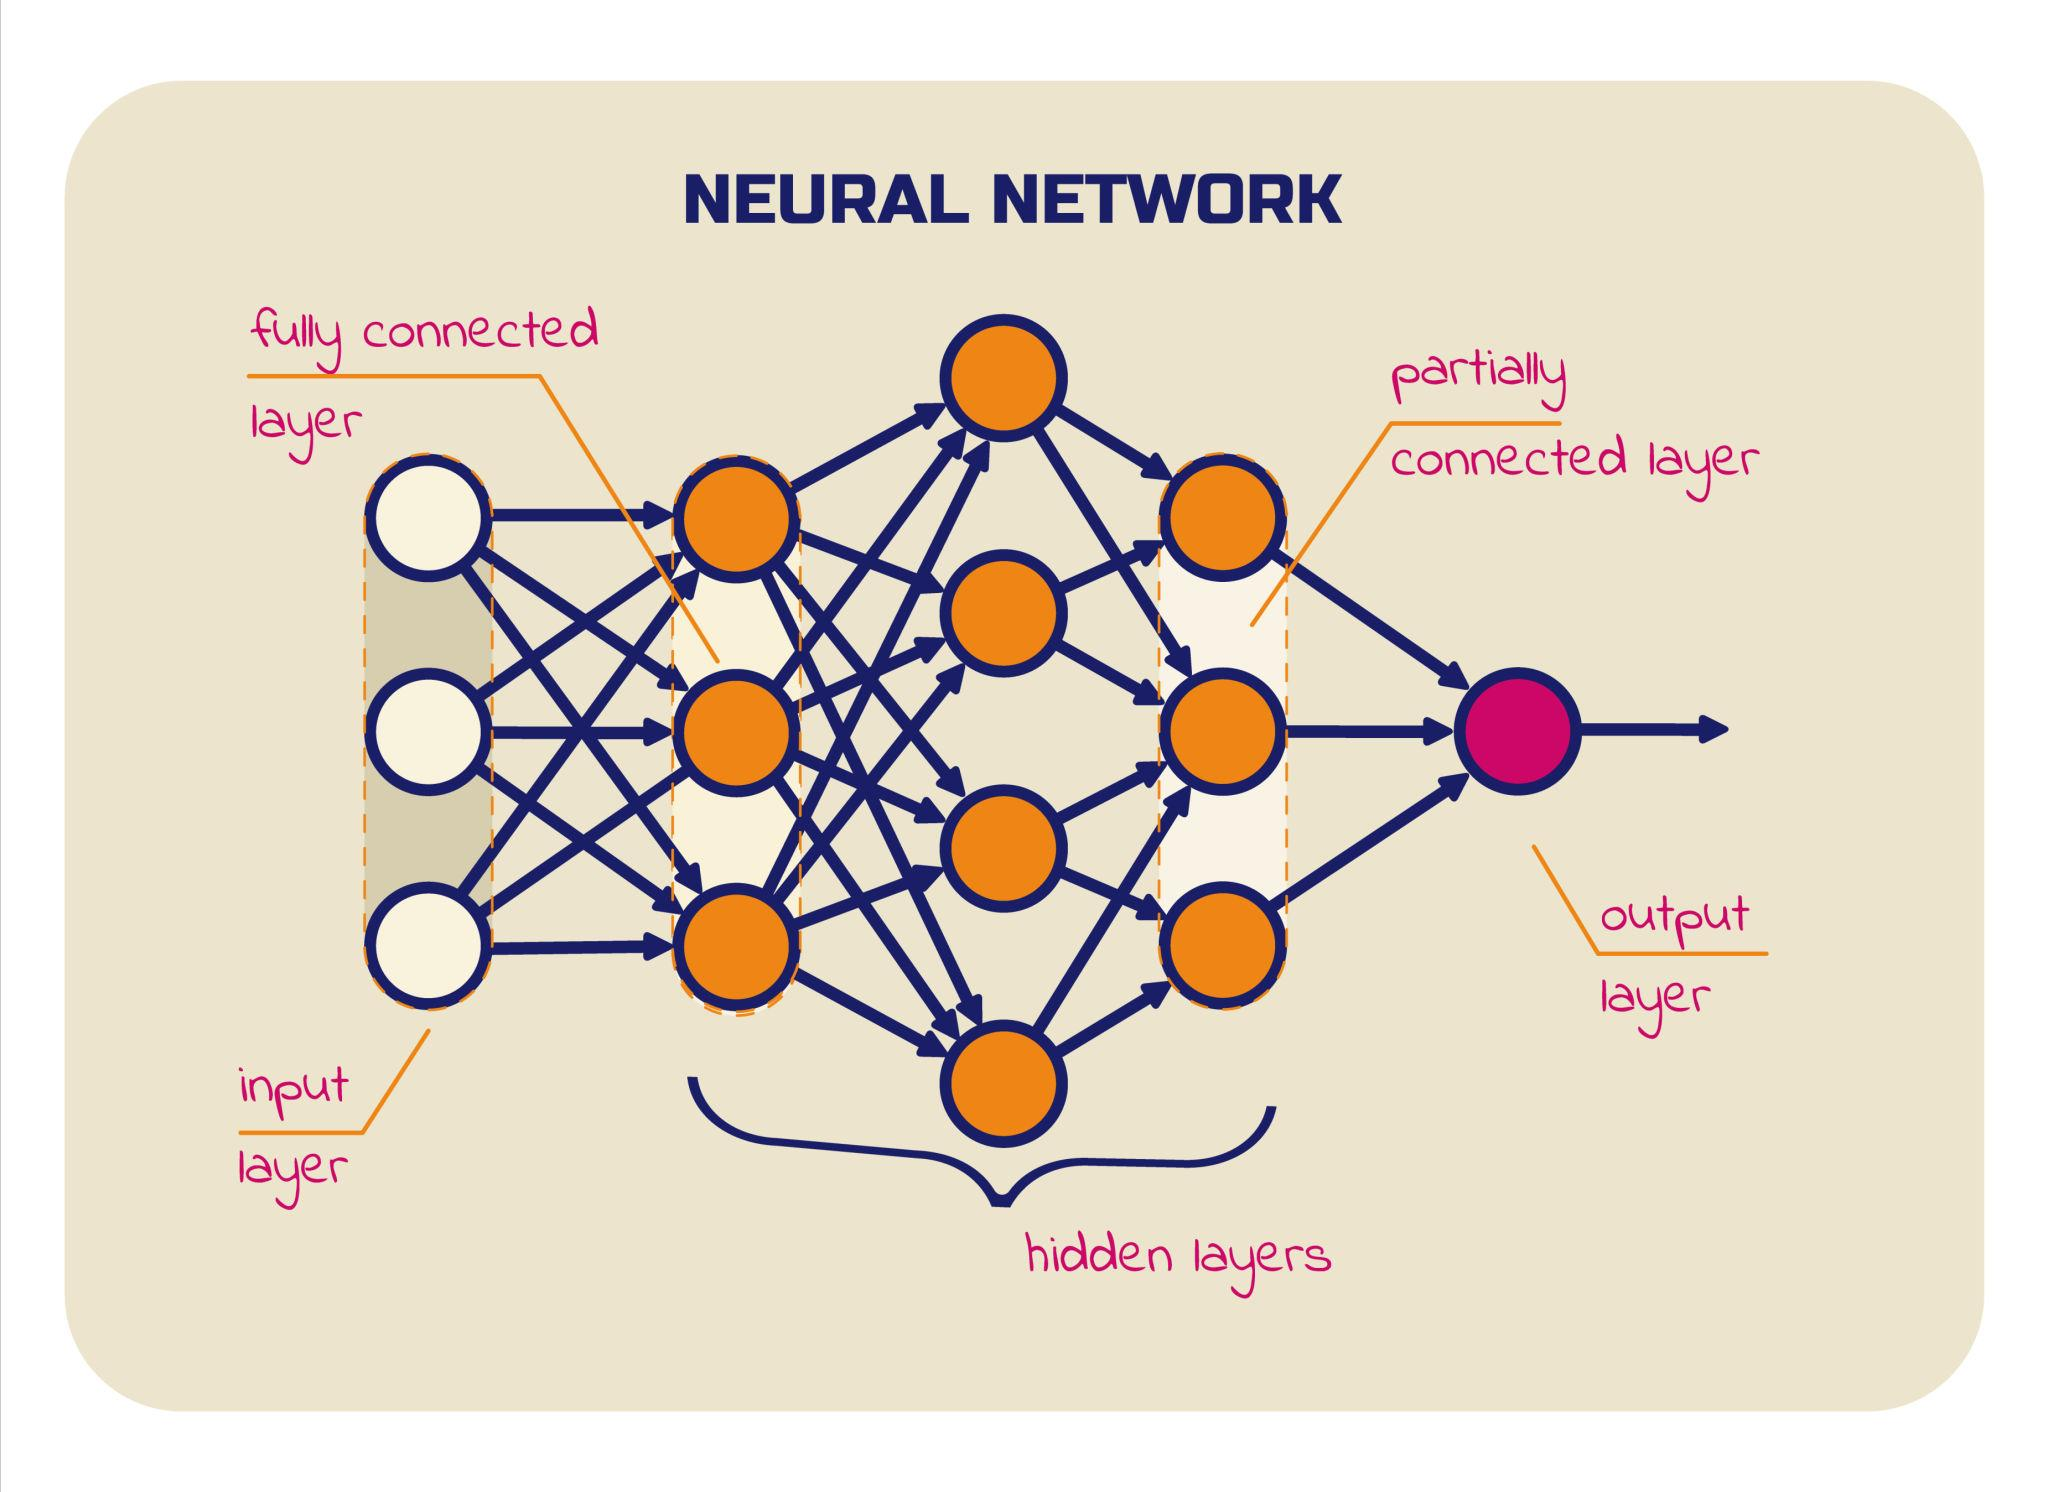
\includegraphics[
    width=0.7\linewidth,
    alt={Feedforward deep neural network with an input layer,
    multiple hidden layers, and an output layer connected sequentially.}
]{plots/dnn_architecture.png}
\caption{Feedforward deep neural network architecture (adapted from \cite{Goodfellow2016}) consisting of an input
layer, multiple hidden layers, and an output layer. Each neuron applies a
weighted linear transformation followed by a nonlinear activation function.}
\label{fig:dnn_architecture}
\end{figure}
\paragraph{Universal approximation and expressiveness.}
A fundamental justification for using neural networks in statistical modeling
is their universal approximation property: sufficiently wide or deep neural
networks can approximate any continuous function on a compact domain to
arbitrary accuracy \cite{Hornik1989,Cybenko1989}. Subsequent work has shown that
depth plays a crucial role in efficiently representing highly nonlinear and
compositional functions, often allowing deep architectures to achieve
exponential gains in representational efficiency over shallow models
\cite{Montufar2014}.

\paragraph{Nonparametric regression in high dimensions.}
From a statistical perspective, DNNs can be viewed as flexible nonparametric
regressors that adapt to unknown smoothness and interaction structures. Unlike
classical kernel or spline methods, whose performance deteriorates rapidly as
the input dimension increases, neural networks can exploit sparsity,
hierarchical structure, and low-dimensional manifolds in high-dimensional
covariates \cite{SchmidtHieber2020}. These properties make DNNs particularly
attractive for estimating conditional expectations or conditional residuals
when the conditioning variable $Z$ is high-dimensional.


\paragraph{Training via backpropagation.}
The parameters of a neural network are typically learned by minimizing a loss
function using gradient-based optimization. Let
\[
\ell:\mathcal{Y}\times\mathbb{R}^m\to\mathbb{R}
\]
denote a loss function that quantifies the discrepancy between an observed
response $y\in\mathcal{Y}$ and the network prediction $f(z;\theta)$.
%\footnote{please define what is $\ell(\cdot)$. it is a loss function?}.
Common choices include the squared-error loss
$\ell(y,\hat y)=(y-\hat y)^2$ for regression and the cross-entropy loss for
classification. Given training observations
$\{(Z_i,Y_i)\}_{i=1}^n$, the network parameters $\theta$ are estimated by
minimizing the empirical risk
\[
\hat L(\theta)
=
\frac{1}{n}\sum_{i=1}^n
\ell\bigl(Y_i,f(Z_i;\theta)\bigr).
\]

Gradients of the loss with respect to network parameters are computed using
\emph{backpropagation}, an efficient application of the chain rule that
propagates derivatives from the output layer back through each hidden layer.
Specifically, let
\[
a_k = \sigma(W_k a_{k-1}+b_k),
\qquad k=1,\ldots,L,
\]
denote the activations at the $k$th layer, where $a_0=z$ is the input vector.
Backpropagation computes the gradients
$\partial \hat L/\partial W_k$ and
$\partial \hat L/\partial b_k$
recursively by propagating error signals from the output layer toward the input
layer. This procedure allows networks with millions of parameters to be trained
efficiently using stochastic optimization.
%\footnote{this $\ell$ is different from the loss function, please change to another notation.}



In practice, neural networks are commonly trained using stochastic gradient
descent (SGD) or its variants. One widely used method is the \emph{Adam}
optimizer \cite{Kingma2015}, which adaptively adjusts learning rates using
estimates of the first and second moments of the gradient. Let $g_t$ denote
the gradient at iteration $t$. Adam updates the parameters using
\[
m_t = \beta_1 m_{t-1} + (1-\beta_1) g_t, \qquad
v_t = \beta_2 v_{t-1} + (1-\beta_2) g_t^2,
\]
followed by bias correction and the parameter update
\[
\theta_{t+1}
=
\theta_t
-
\alpha
\frac{\hat m_t}{\sqrt{\hat v_t}+\epsilon}.
\]
This adaptive learning rate scheme often improves convergence stability and
reduces the need for extensive hyperparameter tuning.

\paragraph{Generalization and regularization.}
Despite their large parameter spaces, DNNs often generalize well when
appropriate regularization strategies are employed. Common approaches include

\begin{itemize}
\item \textbf{Early stopping}: monitoring validation loss and terminating
training before overfitting occurs;
\item \textbf{Weight decay}: penalizing large parameter values through
$\ell_2$ regularization;
\item \textbf{Dropout}: randomly deactivating neurons during training to
reduce co-adaptation among features;
\item \textbf{Sample splitting}: using separate datasets for training and
evaluation to prevent overfitting bias.
\end{itemize}

These techniques effectively control model complexity and help prevent the
network from memorizing training data rather than learning underlying
patterns.

\paragraph{Neural networks for conditional inference.}
In modern causal inference and conditional independence testing, neural
networks are increasingly used as first-stage learners to estimate conditional
means, conditional variances, or conditional distributions
\cite{Chernozhukov2018}. When combined with sample splitting or cross-fitting,
such approaches can mitigate overfitting bias and enable valid downstream
statistical inference, even when the first-stage estimators converge at slower
rates.


While DNNs excel at capturing complex conditional structure, they do not by
themselves provide hypothesis tests or uncertainty quantification. This has
motivated hybrid methodologies that pair neural networks with classical or
distribution-free statistical tools. In the context of conditional
independence testing, neural networks can be leveraged to remove the effect of
high-dimensional confounders, after which principled independence tests are
applied to the resulting residuals. This separation of conditional modeling
and dependence testing forms the foundation of the methodology developed in
this thesis.


\chapter{Adaptive Multiscale Binary Expansion Tests for Independence}
\label{Adaptive_test}
\noindent\textbf{Previously published as:}

Yang, Yang, Ping-Shou Zhong, et al. Adaptive Multiscale Binary Expansion Tests for Independence. Proceedings of the 43rd International Conference on Machine Learning (ICML 2026), Proceedings of Machine Learning Research, 2026.

\section{Background Introduction}

Testing statistical independence between multivariate random variables is a fundamental problem in statistics, econometrics, and machine learning. Beyond classical applications such as feature selection, dimension reduction, and graphical modeling \cite{Cai2018FeatureSM,Waggoner_2021}, independence tests have recently attracted increasing attention in areas including causal discovery \cite{Dai2022IndependenceTA} and large language models \cite{zhu2025independence_icml}.

Classical independence tests, such as the $\chi^2$ test, Fisher’s exact test, and related contingency-table methods \cite{Agresti2013}, have been widely used to assess independence between univariate random variables. However, these approaches can be less powerful and less reliable in multivariate settings. This limitation is driven by small expected cell counts under limited sample sizes and by the rapidly growing number of categories needed to represent multivariate variables \cite{Szekely2007,Gretton2005HSIC}. 

Beyond contingency tables, a broad class of independence tests measures discrepancy between the joint distribution and the product of its marginals. Early examples include Hoeffding’s test of independence \cite{Hoeffding1948} and the related Blum--Kiefer--Rosenblatt coefficient \cite{Blum1961}. Modern developments build on ranks, copulas, and empirical-process ideas to construct distribution-free procedures that are invariant to monotone marginal transformations. Representative examples include consistent rank-based correlations \cite{Bergsma2014,Chatterjee2021}, copula-based goodness-of-fit tests \cite{Genest2004,Kojadinovic2005,Remillard2009}, and the Heller--Heller--Gorfine test \cite{Heller2013}, which aggregates multiscale rank statistics to detect both monotone and nonmonotone dependencies.

Another influential line of work quantifies dependence via the Kullback--Leibler divergence between the joint distribution and the product of marginals, i.e., mutual information. This perspective has motivated $k$-nearest-neighbor estimators \cite{Kraskov2004,Gao2017,Singh2003} and neural estimators \cite{Belghazi2018MINE, Poole2019}
aimed at reducing estimation bias in moderate to high dimensions. More recently, learning- and projection-based paradigms have emerged, including classifier-based reductions \cite{LopezPaz2017,Muandet2017,Kim2019} and projection-based dependence measures \cite{Zhu2017,Weihs2018}. Despite these advances, nonparametric estimation of multivariate joint distributions remains challenging when sample sizes are limited.

Two especially popular nonparametric measures that avoid explicit joint density estimation are based on the Hilbert--Schmidt Independence Criterion (HSIC) \cite{Gretton2008} and distance correlation \cite{Szekely2007,Sejdinovic_2013}. HSIC \cite{Gretton2008} is defined as the Hilbert--Schmidt norm of the cross-covariance operator between random variables mapped into reproducing kernel Hilbert spaces (RKHS). HSIC equals zero if and only if independence holds when the chosen kernels are characteristic (or, more strongly, universal) \cite{Gretton2005HSIC,Sriperumbudur2011Characteristic,Steinwart2012Universal}. Distance correlation \cite{Szekely2007,Sejdinovic_2013} quantifies dependence through a weighted $L_2$ distance between the joint characteristic function and the product of the marginal characteristic functions; its carefully selected weighting yields a dependence measure that is zero if and only if independence holds and is estimable without explicitly estimating characteristic functions. However, as pointed out by one referee, the weight function in distance correlation down weights the high-frequency components in the characteristic functions, which can potentially reduce power for detecting complex, non-linear, and local dependencies.

In this paper, we introduce a new independence measure by representing characteristic functions via binary expansions \cite{zhang2019bet,zhang2021beauty,brown2025belief}. The new independence measure translates an independence testing problem to a cross-covariance testing problem for binary expansion coefficients under a general setting, not limited to RKHS (hence not depending on the choices of kernels). Moreover, by analyzing the distance covariance measure \cite{Szekely2007} from a binary expansion perspective, we discover that the distance covariance measure is equivalent to a weighted quadratic distance between binary expansion coefficients, involving coefficients of binary expansion for all orders. The inclusion of all high-order binary expansion coefficients may introduce more noise than signal, potentially degrading the power of the distance correlation test. The proposed measure has the flexibility to choose resolution so that we can retain only lower-order coefficients to strike a better balance between signal and noise. In addition, the proposed measure substantially improves interpretability by identifying the components that exhibit dependence when the null hypothesis of independence is rejected (see numerical studies for 
an illustration).

Based on this measure, we develop a unified framework for testing weighted cross-covariances between binary-expansion interaction coefficients. A naive construction is computationally infeasible because the number of interaction coefficients grows exponentially with dimension and expansion depth. To address this challenge, we introduce a family of $U$-statistic--based test statistics and derive equivalent kernel representations that reduce computational complexity from $O(2^{dK})$ to $O(dK)$, enabling scalable implementation, where $d$ is the dimension and $K$ is the chosen binary-expansion resolution.

Through weight matrices, the proposed methodology offers additional flexibility and potential power gains. We study two special weighting choices. The first is the identity weight, yielding a baseline test termed the Covariance Binary Expansion Test (CoBET). The second is a distance-correlation--inspired weight, yielding dCoBET, which incorporates positive semidefinite feature weights and establishes a direct link between binary expansions and classical distance-based measures. To adaptively combine complementary weighting schemes, we further introduce wa-dCoBET, which aggregates identity and distance-based weights via sample splitting and foldwise signal-to-noise ratio voting \cite{HeZhongCuiMandrekar2023}.

Simulation studies based on multivariate copulas demonstrate that the proposed methods achieve competitive or superior power across a wide range of linear and nonlinear dependence structures, while remaining computationally efficient and theoretically transparent. The remainder of the chapter is organized as follows. Section~\ref{test procedure} introduces the binary-expansion--based independence measure and the CoBET, dCoBET, and wa-dCoBET statistics, along with their kernel representations and asymptotic distributions. Section~\ref{sec:experiments} presents simulation results, Section~\ref{sec:example} illustrates the method on real data, and Section~\ref{sec:conclusion} concludes. Additional details and technical proofs are provided in the Section ~\ref{theorem_proof}.

\section{Independence Measure and Testing Procedure}
\label{test procedure}

% Given multivariate data arising from complex dependence structures, our goal is
% to construct a testing procedure that is invariant to marginal transformations,
% computationally efficient, and statistically powerful against a broad class of
% alternatives.

Let $\{(X_i,Y_i)\}_{i=1}^n$ be i.i.d.\ copies of $(X,Y)\in\mathbb R^p\times\mathbb R^q$. 
We test
\[
H_0: X\perp Y
\quad \text{vs} \quad
H_1: X\not\perp Y .
\]
% \[
% \begin{aligned}
% H_0:&X\perp Y \Longleftrightarrow F_{XY}(x,y)=F_X(x)F_Y(y),\;\mbox{for all $x,y$} \\
% H_1:&X\not\perp Y \Longleftrightarrow F_{XY}(x,y)\neq F_X(x)F_Y(y),\;\mbox{for some $x,y$}
% \end{aligned}
% \]
where $X\perp Y$ means $X$ is independent of $Y$ and $X \not\perp Y$ means $X$ is not independent of $Y$.
This section will first introduce a new binary expansion based independence measure, and then introduce the proposed $U$--statistic for testing cross-covariance and derive a computationally efficient and scalable kernel 
representation of the proposed statistics, and its asymptotic theory.
Within this framework, we will introduce three tests: the Covariance Binary Expansion Test (CoBET), a distance-covariance weighted multiscale extension (dCoBET), and an adaptive aggregation procedure, wa-dCoBET, which
combines multiple weighting schemes via foldwise signal--to--noise ratio (SNR) voting.


\subsection{A binary expansion based independence measure}
\label{binary_inde}
To simplify our notations, we perform componentwise probability--integral transforms
to $X_i$ and $Y_i$ by $\tilde{U}_i^{(r)} = F_{X^{(r)}}(X_i^{(r)})$ and $\tilde{V}_i^{(s)} = F_{Y^{(s)}}(Y_i^{(s)})$
to obtain random vectors $\tilde{U}_i$ and $\tilde{V}_i$ where 
\[
\tilde{U}_i = (\tilde{U}_i^{(1)},\dots,\tilde{U}_i^{(p)}),
\qquad
\tilde{V}_i = (\tilde{V}_i^{(1)},\dots,\tilde{V}_i^{(q)})
\]
for pairs of samples $(\tilde{U}_i,\tilde{V}_i)$ where $i=1,\cdots,n$ that are independent copies of 
$(\tilde{U},\tilde{V})$. For each transformed coordinate $\tilde{U}_i^{(r)}\in[0,1]$ and $\tilde{V}_i^{(s)}\in[0,1]$,
define $U_i^{(r)}=2\tilde{U}_i^{(r)}-1$
and $V_i^{(s)}=2\tilde{V}_i^{(s)}-1$. It is clear that
\[
\begin{aligned}
X \perp Y \Longleftrightarrow \tilde{U} \perp \tilde{V}
&\Longleftrightarrow
U \perp V.
\end{aligned}
\]
The random vectors $U_i$ and $V_i$ have uniform marginals on $[-1,1]$ and satisfy
$
X_i \perp Y_i \Longleftrightarrow U_i \perp V_i.
$
Independence between $U$ and $V$ admits the classical characterization via
characteristic functions:
\[
U\perp V
\iff
\varphi_{UV}(t,s)=\varphi_U(t)\varphi_V(s),
\quad (t,s)\in\mathbb R^p\times\mathbb R^q .
\]

where $\varphi_{{U}{V}}$ denotes the joint characteristic function and
$\varphi_{U}$, $\varphi_{V}$ denote the marginal characteristic functions.

Consider the binary expansion for ${U}$ and  ${V}$, 
\[
U_i^{(r)}
=
\sum_{k=1}^{\infty} 2^{-k} A^{(r)}_{k,i},
\quad
V_i^{(s)}
=
\sum_{j=1}^{\infty} 2^{-j} B^{(s)}_{j,i},
\]
where $A^{(r)}_{k,i}, B^{(s)}_{j,i}$ are random coefficients that are Bernoulli distributed taking values in $\{-1, +1\}$.
%\footnote{
%When $A^{(r)}_{k,i}$ and $B^{(s)}_{j,i}$ are taking values in $\{-1, +1\}$, the binary expansion should be slightly modified? 
%Maybe also the expression in Theorem 2.1?}
% \[
% A^{(r)}_k := 2U^{(r)}_k - 1 \in \{-1,+1\},
% \\
% B^{(s)}_k := 2V^{(s)}_k - 1 \in \{-1,+1\}.
% \]
We truncate the binary expansions at a finite depth $K\in\mathbb N$, which
controls the \emph{resolution} of the representation. For notational simplicity, we assume the resolution for all the components are $K$.
By approximation theory, we may ignore the remainder term beyond depth $K$; the resulting approximation error
vanishes as $K\to\infty$.

Applying Euler's identity $e^{\jmath z} = \cos z + \jmath\sin z$ yields
\[
e^{\jmath t_r U_i^{(r)}}
=
\prod_{k=1}^{K}
\left\{
\cos\!\left( \frac{t_r}{2^k} \right)
+ \jmath\, A_{k,i}^{(r)} \sin\!\left( \frac{t_r}{2^k} \right)
\right\}, \jmath
=\sqrt{-1}.
\]


Taking expectations gives a polynomial--trigonometric representation of the
marginal characteristic function
\[
\varphi_{U^{(r)}}(t_r)
=
\sum_{a \in \{0,1\}^K}
\psi_a(t_r)\;
\mathbb{E}\!\left(
  \prod_{k=1}^{K}
    (A^{(r)}_k)^{a_k}
\right),
\]
where each coefficient $\psi_a(t_r)$ is formed from products of
$\cos(t_r/2^k)$ and $\sin(t_r/2^k)$. The same construction applies to each
coordinate of $V$.

For a fixed depth $K$, let $I_r$ be the collection of all the non-empty subsets of $\{1,\dots,K\}$. 
Define the multi-index set
\[
\mathcal I_p^*
=\Bigl\{
\begin{aligned}
&I=(I_1,\dots,I_p):
&I_r \subset \{1,\dots,K\},\ I_r\neq\emptyset,\ 1\le r\le p
\end{aligned}
\Bigr\},
\]

and analogously define $\mathcal I_q^*$. Let $|I_r|$ be the cardinality of the set $I_r$.

\begin{theorem}
\label{thm:kernel-representation}
Let $U=(U^{(1)},\dots,U^{(p)})\in[-1,1]^p$ and
$V=(V^{(1)},\dots,V^{(q)})\in[-1,1]^q$ be the componentwise
probability--integral transforms of $X$ and $Y$, and fix a truncation depth
$K\in\mathbb N$.  
For $I\in\mathcal I_p^*$, write $|I|=\sum_{r=1}^p |I_r|$ and define
\[
\Pi_I(t)
=
\prod_{r=1}^p
\Bigl(
\prod_{l\in I_r}\sin\frac{t_r}{2^l}
\prod_{l\notin I_r}\cos\frac{t_r}{2^l}
\Bigr),
\qquad t\in\mathbb R^p,
\]
with $\Pi_J(s)$ defined analogously for $J\in\mathcal I_q^*$. Then
\[
\varphi_{UV}(t,s)-\varphi_U(t)\varphi_V(s)
=
\sum_{I\in\mathcal I_p^*}\sum_{J\in\mathcal I_q^*}
\jmath^{|I|+|J|}\,
m_{I,J}\,\Pi_I(t)\,\Pi_J(s),
\]
where $I=(I_1,\ldots,I_p)\in\mathcal I_p^\star$ and $J=(J_1,\ldots,J_q)\in\mathcal I_q^\star$,
with $I_r,J_s\subseteq\{1,\ldots,K\}$, and
\[
\begin{aligned}
m_{I,J}
&=\mathbb E(\mathcal A_{i,I}\mathcal B_{i,J})
-\mathbb E(\mathcal A_{i,I})\,\mathbb E(\mathcal B_{i,J}),\\
\mathcal A_{i,I}
&=
\prod_{r=1}^p\prod_{k\in I_r} A^{(r)}_{k,i},
\qquad
\mathcal B_{i,J}
=
\prod_{s=1}^q\prod_{j\in J_s} B^{(s)}_{j,i}.
\end{aligned}
\]

\end{theorem}

The proof of Theorem \ref{thm:kernel-representation} is included in section \ref{sec:proof-kernel-representation}. 
The expansion in Theorem \ref{thm:kernel-representation} is related to the universal binary expansion approximation of characteristic functions developed in \citep{zhang2019bet,zhang2021beauty}. 
Compared to these results, Theorem \ref{thm:kernel-representation} can be viewed as a corresponding decomposition of independence: The essential difference
$\varphi_{UV}(t,s)-\varphi_U(t)\varphi_V(s)$ is expressed as a finite linear combination of cross-covariance coefficients
$m_{I,J}=\mbox{Cov}(\mathcal{A}_{i,I},\mathcal{B}_{i,J})$ with basis functions $\Pi_I(t)\Pi_J(s)$.

This covariance form is crucial in the multivariate setting, since within-vector dependence generally implies nonzero marginal interaction means, and therefore any form of dependence is naturally characterized by all cross-covariances $\{m_{I,J}\}$. 
As a direct consequence, testing $U \perp V$ reduces to testing whether the collection $\{m_{I,J}\}$ vanishes. 
This translates the independent testing problem into a covariance test problem, which is an easier problem. 
More specifically, define the feature vectors
\[
\vec A_i=(\mathcal{A}_{i,I})_{I\in\mathcal I_p^\star}\in\mathbb R^{\,d_A},
\quad
\vec B_i=(\mathcal{B}_{i,J})_{J\in\mathcal I_q^\star}\in\mathbb R^{\,d_B},
\]
with $d_A=2^{pK}-1$, $d_B=2^{qK}-1$
and define the cross-covariance matrix
\[
\Sigma_{AB}=\operatorname{Cov}(\vec A_i,\vec B_i),
\qquad
\Sigma_{BA}=\Sigma_{AB}^\top.
\]
A specific example of $\mathcal I_p^*$, and $\vec A_i$ is given in the section \ref{app:binary-example-new}

The results in Theorem \ref{thm:kernel-representation} imply that 
$U$ and $V$ are independent if and only if $\Sigma_{AB}=0$.
The binary expansion feature vectors $\vec A$ and $\vec B$ have dimensions $d_A=2^{pK}-1$
and $d_B=2^{qK}-1$, which grows exponentially fast as $K$ and $p$ or $q$ grow. 
Fortunately, this only serves as a theoretical expression for easy understanding. 
The proposed procedures do NOT construct it explicitly and hence it overcomes the computation issues of using $\vec A$ and $\vec B$ directly. See Section \ref{subsec:cobet} for details.

More generally, define a measure of independence between joint characteristic function and marginal characteristic functions 
\[
\mathcal V^2(U,V)
=\int_{\mathbb R^p}\int_{\mathbb R^q} |\varphi_{UV}(t,s)-\varphi_U(t)\varphi_V(s)|^2w^2(t,s)dtds,
\]
where $w^2(t,s)$ is a non-negative weight function. This weight measure includes
distance covariance measure as a special case. 
We write $\mathcal V^2(U,V)$ as $\mathcal V_W^2(U,V)$ if the weight $w(t,s)=w_0(t)w_1(s)$ is applied and
write $\mathcal V^2(U,V)$ as $\mathcal V_D^2(U,V)$ if 
the distance-covariance weight $w^2(t,s)=1/\{\|t\|^{p+1}\|s\|^{q+1}\}$ \cite{Szekely2007} is used. 
Applying Theorem \ref{thm:kernel-representation}, 
we have
\begin{align*}
\mathcal V_W^2(U,V)&=\sum_{I,I'\in\mathcal I_p}\sum_{J,J'\in\mathcal I_q}
m_{I,J}\,W^{(p)}_{I,I'}\,W^{(q)}_{J,J'}\,m_{I',J'}\\
&=\mbox{tr}(\Sigma_{AB}W_B\Sigma_{BA}W_A),
\end{align*}
where the weight matrix
$
W_A=(W^{(p)}_{I,I'})_{I,I'\in\mathcal I_p^\star}
\in\mathbb R^{\,d_A\times d_A}
$
has entries
\[
W^{(p)}_{I,I'}
=
\int_{\mathbb R^p}
\Pi_I(t)\,\Pi_{I'}(t)\,w_0^2(t)\,dt.
\]
The weight matrix $W_B\in\mathbb R^{d_B\times d_B}$ is defined analogously to $W_A$ by replacing
$p,\mathcal I_p^\star,\Pi_I(t), w_0(t)$ with $q,\mathcal I_q^\star,\Pi_J(s)$ and $w_1(s)$.

If one chooses the distance-covariance weight~\cite{Szekely2007}, the resulting
population distance covariance $\mathcal V_D^2(U,V)$ admits
\[
\mathcal V_D^2(U,V)
=
\operatorname{tr}\!\left(
\Sigma_{AB}\,K^{(q)}\,\Sigma_{BA}\,K^{(p)}
\right),
\]
where for $d\in\{p,q\}$,
\[
K^{(d)}_{I,I'}
=
\frac{1}{c_d}
\int_{\mathbb R^d}
\frac{\Pi_I(t)\Pi_{I'}(t)}{\|t\|^{d+1}}\,dt,
\qquad
I,I'\in\mathcal I_d^\star.
\]
where $c_d$ is a constant. Both $K^{(p)}$ and $K^{(q)}$ are symmetric positive semidefinite with closed-form expressions depending only on $(p,K)$ and $(q,K)$, respectively; no numerical integration is required (section \ref{computational_simp}). When $K$ is large, $\mathcal V_{D,K}^2(U,V)$ converges to its
limit distance covariance measure $\mathcal V_{D}^2(U,V)$.


\subsection{Covariance Binary Expansion Tests}
\label{subsec:cobet}


Theorem~\ref{thm:kernel-representation} shows that departures from independence
between $U$ and $V$ are fully characterized by the collection of covariances
$\{m_{I,J}\}_{I\in\mathcal I_p^\star,\;J\in\mathcal I_q^\star}$.
Equivalently, independence is characterized by the vanishing of the
cross--covariance matrix or the distance measures $\mathcal V_W^2(U,V)$
defined in Section \ref{binary_inde}.

The simplest dependence measure aggregates all 
binary--expansion interactions
with identity weights $w_0(t)=1$ and $w_1(s)=1$ in 
$\mathcal V_W^2(U,V)$ defined in Section \ref{binary_inde}, write it as
$\mathcal V_I^2(U,V)$. More specifically, 
define the population functional
\[
\mathcal V_I^2(U,V)
=
\operatorname{tr}\!\bigl(\Sigma_{AB}\Sigma_{BA}\bigr)
:=
\|\Sigma_{AB}\|_{\mathrm F}^2.
\]

The corresponding sample statistic to estimate $\mathcal V_I^2(U,V)$ 
is constructed as an unbiased $U$--statistic,
defined below $T_n^{(W)}$ with $W_A$ and $W_B$ identity matrices, 
and is referred to as the \emph{Covariance Binary Expansion Test (CoBET)}.


More generally, let $W_A$ and $W_B$ be
matrices defined in Section \ref{binary_inde} of sizes, respectively, $d_A\times d_A$ and
$d_B\times d_B$.
The corresponding population quadratic functional
\begin{equation*}
\begin{aligned}
\mathcal V_W^2(U,V)
&=
\operatorname{tr}\!\bigl(
\Sigma_{AB} W_B \Sigma_{BA} W_A
\bigr).
%\\[0.3em]
%\Sigma_{BA}
%&=
%\Sigma_{AB}^\top .
\end{aligned}
\end{equation*}

By Theorem~\ref{thm:kernel-representation}, $\mathcal V_W^2(U,V)=0\Longleftrightarrow H_0: U\perp V$  
for any non-negative definite matrices $W_A,W_B$ defined in Section \ref{binary_inde}. Choosing distance-covariance motivated weights (e.g., $W_A=K^{(p)}$, $W_B=K^{(q)}$)
yields the \emph{dCoBET} family. Although dCoBET and distance covariance share similar weight function, distance covariance is only equivalent to dCoBET when $K$ is large enough, but dCoBET has the flexibility to truncate the binary expansion to remove independent components with high-variant.

\paragraph{Unbiased $U$--statistics for CoBET and dCoBET}
Given i.i.d.\ samples $\{(U_i,V_i)\}_{i=1}^n$, and recall that the binary expansion interaction 
coefficient vectors
$\vec A_i=(A_{i,I})_{I\in\mathcal I_p^\star}$ and
$\vec B_i=(B_{i,J})_{J\in\mathcal I_q^\star}$ in Section \ref{binary_inde}.
% Write
% \[
% \vec A_i = \tilde A_i + \mu_A,
% \qquad
% \vec B_i = \tilde B_i + \mu_B,
% \]
% where $\mu_A=\mathbb E(\vec A)$ and $\mu_B=\mathbb E(\vec B)$.
Define
\[
T_n^{(W)} = T_{1n}^{(W)} - 2T_{2n}^{(W)} + T_{3n}^{(W)},
\] with
\begin{align*}
T_{1n}^{(W)} &=
\frac{1}{n(n-1)}\sum_{i\ne j}
(\vec A_i^\top W_A \vec A_j)
(\vec B_j^\top W_B \vec B_i),\\
T_{2n}^{(W)} &=
\frac{1}{\binom{n}{3}}\sum_{i\ne j\ne k}
(\vec A_i^\top W_A \vec A_j)
(\vec B_j^\top W_B \vec B_k),\\
T_{3n}^{(W)} &=
\frac{1}{\binom{n}{4}}\sum_{i\ne j\ne k\ne\ell}
(\vec A_i^\top W_A \vec A_j)
(\vec B_k^\top W_B \vec B_\ell),
\end{align*}
where $\binom{n}{k}$ is a binomial coefficient with $k\leq n$. The second and third terms $T_{2n}^{(W)}$ and $T_{3n}^{(W)}$ are used to cancel the non-zeros means in the vectors $\vec A_i$ and $\vec B_i$ so that (see the proof in the Section \ref{sec:Ustat-weighted})
\[ \mathbb E\!\left\{T_n^{(W)}\right\} = \mathcal V_W^2(U,V). \]
Although the second and third terms  $T_{2n}^{(W)}$ and $T_{3n}^{(W)}$ involve summations over $O(n^3)$ and $O(n^4)$ terms, respectively, they can be computed at the order of $O(n^2)$ (See the details in the Section \ref{computational_simp}).
The construction of $T_n^{(W)}$ is motivated by \cite{CZZ2010} 
but an essential and crucial difference is we do NOT have $\vec A_i$ and $\vec B_i$ available,
because $\vec A_i$ and $\vec B_i$ have dimensions $d_A=2^{pK}-1$ and $d_B=2^{qK}-1$, which grows exponentially fast as $K$ and $p$ or $q$ grows and hence constructing them explicitly is computationally infeasible. 
Thus, the format in $T_n^{(W)}$ only serves for analyzing its theoretical property. 

To compute the proposed CoBET and dCoBET statistics, we note that $T_n^{(W)}$ depends on the terms such as $\vec A_i^\top \vec A_j$ (when $W_A=I_{d_A}$) and 
$\vec A_i^\top W_A \vec A_j$. The following theorem shows how to compute them
at the order of $O(pK)$. 

\begin{theorem}
\label{thm:computeATA}
For any $i\neq j$,
\begin{equation}
\label{eq:A-dot-factorization}
\vec A_i^\top \vec A_j
=
\prod_{r=1}^p\prod_{k=1}^K
\bigl(1 + A^{(r)}_{k,i}A^{(r)}_{k,j}\bigr)
-1 .
\end{equation}
Moreover,
\begin{align*}
\vec A_i^\top W_A \vec A_j
&=
\int_{\mathbb R^p}
C^2(t)
\left\{
\prod_{r=1}^p\prod_{k=1}^K
\bigl(1+A^{(r)}_{k,i}\pi_k^{(r)}(t_r)\bigr)
-1
\right\}
\\
&\quad\times
\left\{
\prod_{r=1}^p\prod_{k=1}^K
\bigl(1+A^{(r)}_{k,j}\pi_k^{(r)}(t_r)\bigr)
-1
\right\}
w_0^2(t)\,dt ,
\end{align*}

where
$C^2(t)=\prod_{r=1}^p\prod_{k=1}^K \cos^2(t_r/2^k)$
and
$\pi_k^{(r)}(t_r)=\tan(t_r/2^k)$.
\end{theorem}
Proof of Theorem~\ref{thm:computeATA} is given in Section \ref{proof_theorem2.2}.
Equation~\eqref{eq:A-dot-factorization} shows that the CoBET kernel
$\vec A_i^\top \vec A_j$ can be evaluated in $O(pK)$ time using only pairwise
bit products, despite the exponentially growing ambient dimension of $\vec A_i$.
Similarly, evaluating $\vec A_i^\top W_A \vec A_j$ via the representation in
Theorem~\ref{thm:computeATA} reduces to forming the $O(pK)$ products inside the
braces for each integration point $t$, rather than enumerating the
$2^{pK}-1$ interaction coordinates.
Analogous results hold for $\vec B_i^\top \vec B_j$ (when $W_B=I_{d_B}$)
and for $\vec B_i^\top W_B \vec B_j$. In particular, 
if $w_0^2(t)=\prod _{r=1}^p w_{0r}^2(t_r)$, we can further write
$\vec A_i^\top W_A \vec A_j$ as a product of marginal integrations, 
which can be computed even more efficiently. See the Section \ref{proof_theorem2.2} for the details.

The following Theorem \ref{lem:leadingordervar} provides the leading order variance of the test statistic $T_{n}^{(W)}$.

\begin{theorem}
\label{lem:leadingordervar} 
Under the null hypothesis $H_0: U\perp V$, the leading order variance of $T_n^{(W)}$ 
is
\begin{equation}
\label{eq:var-leading-general}
\Var\!\big(T_n^{(W)}\big)
= \frac{2}{n(n-1)}
  \|W_A\Sigma_A\|_{\mathrm F}^2
  \|W_B\Sigma_B\|_{\mathrm F}^2
  \,\{1+o(1)\}.
\end{equation}
\end{theorem} 
For CoBET ($W_A=I_{d_A}, W_B=I_{d_B}$), \eqref{eq:var-leading-general} reduces to 
$ \Var(T_{n}^{(W)}) = 2\|\Sigma_A\|_F^2\|\Sigma_B\|_{\mathrm F}^2/\{n(n-1)\} . $
To estimate the leading order variance, a ratio-consistent estimator can be obtained by 
using U-statistics that are similar to the construction of the test statistic
$T_n^{(W)}$. More specifically, we can estimate $\|W_A\Sigma_A\|_{\mathrm F}^2$ by
\begin{align*}
\widehat{\|W_A\Sigma_A\|_{\mathrm F}^2}
&= \frac{1}{n(n-1)}\sum_{i\ne j}
(\vec A_i^\top W_A \vec A_j)^2\\
&-\frac{2}{\binom{n}{3}}\sum_{i\ne j\ne k}
(\vec A_i^\top W_A \vec A_j)
(\vec A_j^\top W_A \vec A_k)\\
&+ \frac{1}{\binom{n}{4}}\sum_{i\ne j\ne k\ne\ell}
(\vec A_i^\top W_A \vec A_j)
(\vec A_k^\top W_A \vec A_\ell).
\end{align*}
An estimator of $\|W_B\Sigma_B\|_{\mathrm F}^2$ can be constructed similarly. %to $\widehat{\|W_A\Sigma_A\|_{\mathrm F}^2}$. 
Note that both estimators $\widehat{\|W_A\Sigma_A\|_{\mathrm F}^2}$ and $\widehat{\|W_B\Sigma_B\|_{\mathrm F}^2}$ depend
only on the terms like $\vec A_i^\top \vec A_j$ and $\vec A_i^\top W_A \vec A_j$,
which can be computed efficiently using Theorem \ref{thm:computeATA} without
expanding $\vec A_i$ and $\vec B_i$ explicitly.
The following Theorem \ref{thm:weighted-clt} establishes
the limiting distribution of dCoBET and CoBET statistics
under the null hypothesis.

\begin{theorem} 
\label{thm:weighted-clt}  Assume $\{(U_i,V_i)\}_{i=1}^n$ are i.i.d. random vector pairs, and $W_A, W_B$ are deterministic symmetric matrices. 
%\[ \mathbb E\|\tilde A_i\|^4<\infty, \qquad \mathbb E\|\tilde B_i\|^4<\infty. \] 
Assume the binary expansion depth $K=K(n)\to\infty$ as $n\to\infty$.
%= \frac{2}{n(n-1)}\, \mathbb E\!\left[h_{W,n}(Z_1,Z_2)^2\right], \] 
Let $\widehat{\Var}(T_n^{(W)})$ be a ratio-consistent estimator of $\Var(T_n^{(W)})$. If $\mbox{tr}\{(\Sigma_AW_A)^4\}=o\Big[\mbox{tr}^2\{(\Sigma_AW_A)^2\}\Big]$ and $\mbox{tr}\{(\Sigma_BW_B)^4\}=o\Big[\mbox{tr}^2\{(\Sigma_BW_B)^2\}\Big]$, under $H_0: U \perp V$, then
\[ Z_n^{(W)} := \frac{T_n^{(W)}}{\sqrt{\widehat{\Var}(T_n^{(W)})}} \;\stackrel{d}{\Rightarrow}\; \mathcal N(0,1),
\]
where $\stackrel{d}{\Rightarrow}$ denotes converging in distribution.
\end{theorem}


Theorem~\ref{thm:weighted-clt} establishes the asymptotic normality of
$T_n^{(W)}$ under the null hypothesis, where the statistic is degenerate and
its limiting distribution is driven by second--order fluctuations after
proper normalization. We now turn to the behavior of $T_n^{(W)}$ under the
alternative hypothesis $H_1:U\not\!\perp V$, where this degeneracy no longer
holds. In this case, the leading contribution arises from the first--order
projection of the underlying kernel, resulting in a classical $\sqrt{n}$--rate
central limit theorem with a different variance structure.


\begin{theorem}[Asymptotic normality under alternatives]
\label{thm:alt-clt}
Let $\{(U_i,V_i)\}_{i=1}^n$ be i.i.d.\ random vector pairs. Let
$\vec A_i$ and $\vec B_i$ denote the corresponding binary expansion feature
vectors, and define
\[
  \tilde A_i=\vec A_i-\mathbb E(\vec A_i),
  \qquad
  \tilde B_i=\vec B_i-\mathbb E(\vec B_i),
  \qquad
  Z_i=(\tilde A_i,\tilde B_i).
\]
Let $W_A$ and $W_B$ be deterministic symmetric weight matrices, and define
\[
  h(Z_i,Z_j)
  =
  (\tilde A_i^\top W_A\tilde A_j)
  (\tilde B_i^\top W_B\tilde B_j),
  \qquad i\ne j.
\]
Let
\[
  \theta_W
  =
  \mathbb E\{h(Z_1,Z_2)\}
  =
  \operatorname{tr}(W_A\Sigma_{AB}W_B\Sigma_{BA}),
\]
where $\Sigma_{AB}=\mathbb E(\tilde A\tilde B^\top)$ and
$\Sigma_{BA}=\Sigma_{AB}^\top$.
Define the first-order Hoeffding projection
\[
  \psi(Z_1)
  =
  \mathbb E\{h(Z_1,Z_2)\mid Z_1\}-\theta_W
  =
  \tilde A_1^\top W_A\Sigma_{AB}W_B\tilde B_1-\theta_W,
\]
and let $\sigma_{1,W}^2=\operatorname{Var}\{\psi(Z_1)\}$,
with $0<\sigma_{1,W}^2<\infty$. Assume:
\begin{itemize}
  \item[\upshape(A1)] $\operatorname{Var}(T_{2n}^{(W)})+\operatorname{Var}(T_{3n}^{(W)})
        = o\!\left\{\operatorname{Var}(T_{1n}^{(W)})\right\}$;
  \item[\upshape(A2)] the Lindeberg condition holds for the array
        $\bigl\{D_{n,i} = \tfrac{2}{n}\psi(Z_i)\bigr\}_{i=1}^n$.
\end{itemize}
Then, under any alternative for which $\Sigma_{AB}\ne 0$,
\[
  \mathbb E\{T_n^{(W)}\}=\theta_W,
  \qquad
  \operatorname{Var}\{T_n^{(W)}\}=\frac{4\sigma_{1,W}^2}{n}\{1+o(1)\},
\]
and
\[
  \sqrt{n}\bigl(T_n^{(W)}-\theta_W\bigr)
  \stackrel{d}{\longrightarrow}
  N\bigl(0,\,4\sigma_{1,W}^2\bigr).
\]
\end{theorem}

\begin{remark}
Condition~\textup{(A1)} is implied by the trace bound
\[
  \operatorname{tr}(W_A\Sigma_AW_A\Sigma_A)\,
  \operatorname{tr}(W_B\Sigma_BW_B\Sigma_B)
  = o(n\sigma_{1,W}^2),
\]
where $\Sigma_A=\operatorname{Cov}(\tilde A)$ and
$\Sigma_B=\operatorname{Cov}(\tilde B)$.
Condition~\textup{(A2)} is implied by the Lyapunov moment condition
$\mathbb E\{\psi^4(Z_1)\}=o(n\sigma_{1,W}^4)$,
and holds automatically when $K=O(\log n)$ and the binary expansion
features are bounded, since $\psi(Z_1)$ is then bounded uniformly in $n$.
\end{remark}
% Assume that
% \[
% 0<\sigma_{1,W}^2<\infty.
% \]
% Furthermore, assume the remainder terms in the Hoeffding decomposition are
% asymptotically negligible, namely
% \[
% \frac{
% \operatorname{tr}(W_A\Sigma_AW_A\Sigma_A)
% \operatorname{tr}(W_B\Sigma_BW_B\Sigma_B)
% }{
% n\sigma_{1,W}^2
% }
% \to 0,
% \tag{A1}
% \]
% where
% \[
% \Sigma_A=\operatorname{Cov}(\tilde A),
% \qquad
% \Sigma_B=\operatorname{Cov}(\tilde B),
% \]
% and assume the Lyapunov-type condition
% \[
% \frac{\mathbb E\{\psi^4(Z_1)\}}{n\sigma_{1,W}^4}\to 0.
% \tag{A2}
% \]

% Then, for the weighted statistic $T_n^{(W)}$, under any alternative for which
% $\Sigma_{AB}\ne 0$ and the above conditions hold,
% \[
% \mathbb E\{T_n^{(W)}\}=\theta_W,
% \]
% and
% \[
% \operatorname{Var}\{T_n^{(W)}\}
% =
% \frac{4\sigma_{1,W}^2}{n}\{1+o(1)\}.
% \]
% Moreover,
% \[
% \frac{
% T_n^{(W)}-\theta_W
% }{
% \sqrt{\operatorname{Var}\{T_n^{(W)}\}}
% }
% \stackrel{d}{\longrightarrow}
% N(0,1).
% \]
% Equivalently,
% \[
% \sqrt n\bigl(T_n^{(W)}-\theta_W\bigr)
% \stackrel{d}{\longrightarrow}
% N\bigl(0,4\sigma_{1,W}^2\bigr).
% \]
% \end{theorem}



\subsection{Weighted Aggregated dCoBET (wa-dCoBET)}
\label{subsec:wa-dcobet}

CoBET and dCoBET are constructed using different weighting matrices. Although both weighting matrices maintain the type I error under the null,  
the power of tests may depend on the choice of weighting matrices
due to the underlying dependence structure. To make our procedure adaptive to weight matrices, we introduce a \emph{weighted aggregated
dCoBET} (wa-dCoBET) statistic, which automatically selects and blends multiple weighting schemes using a data-driven signal-to-noise ratio (SNR) criterion \cite{HeZhongCuiMandrekar2023}.

We consider two positive weight pairs
$W^{(\mathrm{id})} = \bigl(I_{d_A},\, I_{d_B}\bigr)$, 
$W^{(D)} = \bigl(K^{(p)},\, K^{(q)}\bigr),$
corresponding to the identity weighted CoBET choice and the distance-covariance-weighted dCoBET choice, respectively. See Section 2.2 for
details. For chosen $W=(W_A,W_B)$, let $T_n^{(W)}$ and $Z_n^{(W)}$ denote the corresponding $U$--statistic and its standardized version  defined in Section~\ref{subsec:cobet}, with variance estimated using estimator given in Section~\ref{subsec:cobet}. More specifically, $Z_n^{(\mathrm{id})}$ is
the standardized statistic with identity weight $W=W^{(id)}$ (CoBET)
and $Z_n^{(D)}$ is
the standardized statistic with distance covariance motivated weight $W=W^{(D)}$ (dCoBET).

\paragraph{Foldwise SNR voting.}
We split the data into $M$ folds (e.g., $M=10$) and compute foldwise standardized
statistics $\mathrm{SNR}_{n,m}^{(\mathrm{id})}$ and $\mathrm{SNR}_{n,m}^{(D)}$.
Each fold votes for the weighting with the larger SNR, yielding empirical
weights
$w_{\mathrm{id}}=\frac1M\sum_{m=1}^M
\mathbf 1\{\mathrm{SNR}_{n,m}^{(\mathrm{id})}>\mathrm{SNR}_{n,m}^{(D)}\}$,
with $w_D=1-w_{\mathrm{id}}$.

where $\mathrm{SNR}_{n,m}^{(\mathrm{id})}$ and $\mathrm{SNR}_{n,m}^{(D)}$ denote
the estimated signal--to--noise ratios based on
$Z_{n,m}^{(\mathrm{id})}$ and $Z_{n,m}^{(D)}$, respectively.

The empirical vote proportions are used to form the aggregated weights
$
W_A^{(\mathrm{agg})}
= w_{\mathrm{id}}\,I_{d_A} + w_D\,K^{(p)}$ and 
$W_B^{(\mathrm{agg})}
= w_{\mathrm{id}}\,I_{d_B} + w_D\,K^{(q)}.
$
Evaluating the statistic with these aggregated weights yields the final
standardized statistic $Z_n^{(\mathrm{agg})}$.
% \[
% Z_n^{(\mathrm{agg})}
% =
% \frac{T_n^{(W^{(\mathrm{agg})})}}
% {\sqrt{\widehat{\Var}\!\left(T_n^{(W^{(\mathrm{agg})})}\right)}}.
% \]

The procedure strictly generalizes CoBET and dCoBET: setting
$w_{\mathrm{id}}=1$ recovers CoBET, while $w_D=1$ recovers dCoBET with
$(K^{(p)},K^{(q)})$. 
% Since $W^{(\mathrm{agg})}$ is a convex combination of PSD
% matrices, the statistic and its plug--in variance remain nonnegative. 
Foldwise
SNR voting provides adaptivity while mitigating overfitting. When the number of folds $M$ is large, the estimated $\hat{w}_{id}$ and $\hat{w}_{D}$ converge (in probability) to their limits ${w}_{id}$ and ${w}_{D}$. Hence, the aggregated weight $\hat{W}_A^{(\mathrm{agg})}$ converges in probability to its limit $W_A^{(\mathrm{agg})}$. Then, applying Theorem \ref{thm:weighted-clt} and the Slutsky Theorem, under
$H_0: U \perp V$ and $K=K(n)\to\infty$,
$
Z_n^{(\mathrm{agg})} \stackrel{d}{\Rightarrow} \mathcal N(0,1)
\quad \text{as}\quad n\to\infty,
$
yielding an asymptotically level-$\alpha$ test.
For details of wa-dCoBET, please refer to Algorithm~\ref{alg:wa-dcobet-compact}. 

The resolution hyperparameter $K$ could be selected in a data-driven manor by maximizing the SNR of the power function. To provide practical guidelines and investigate the robustness of the proposed method to $K$, we conducted a sensitivity analysis in section~\ref{choose_k}.

If the null hypothesis is rejected, the source of dependence can be further investigated by adding an additional step. Specifically, when the dimensions of the random vectors are moderate, the global statistic can be decomposed into a sum of marginal statistics and their interactions. In higher-dimensional settings, such a decomposition may not be feasible. Instead, one can assess the contribution of each dimension to the aggregated adaptive statistic by removing one dimension at a time and ranking their relative importance. This ranking would provide useful insights into the underlying dependence structure.
yielding an asymptotically level-$\alpha$ test.

\begin{algorithm}[ht]
\raggedright
\caption{wa-dCoBET via 10-fold SNR voting}
\label{alg:wa-dcobet-compact}
\DontPrintSemicolon
\KwIn{Samples $\{(U_i,V_i)\}_{i=1}^n$ with $U_i,V_i\in\mathbb{R}^p$; depth $K$; folds $M=10$; base weights $W^{(\mathrm{id})}=I_{d_K}$, $W^{(J)}=K^{(p)}$; level $\alpha$.}
\KwOut{Standardized statistic $Z^{(\mathrm{agg})}$ and decision $\mathbf{1}\{Z^{(\mathrm{agg})}>z_{1-\alpha}\}$.}

\textbf{Features.}
Construct centered binary-expansion features $A_i,B_i\in\mathbb{R}^{d_K}$ at depth $K$ and their sample covariances $\hat\Sigma_A,\hat\Sigma_B$.\;

\textbf{Fold split.}
Partition $\{1,\dots,n\}$ into $M$ disjoint folds $F_1,\dots,F_M$ (nearly equal sizes).\;

\textbf{Foldwise SNRs.}
\For{$m=1$ \KwTo $M$}{
  Using only indices in $F_m$, compute $Z_m^{(\mathrm{id})}$ and $Z_m^{(J)}$ where
  $Z_m^{(W)} := T^{(W)}(F_m) \big/ \sqrt{\widehat{\mathrm{Var}}(\tilde T_1^{(W)})(F_m)}$.\; \\
  Record $S_m \gets \arg\max\{Z_m^{(\mathrm{id})}, Z_m^{(J)}\}$.\;
}

\textbf{Aggregate weights.}
Set $w_{\mathrm{id}} \gets \frac{1}{M}\sum_{m=1}^M \mathbf{1}\{S_m=\mathrm{id}\}$, $w_J \gets 1-w_{\mathrm{id}}$.\; \\
Form blended PSD weights
$W_A^{(\mathrm{agg})} \gets w_{\mathrm{id}} W_A^{(\mathrm{id})} + w_J W_A^{(J)}$,
$W_B^{(\mathrm{agg})} \gets w_{\mathrm{id}} W_B^{(\mathrm{id})} + w_J W_B^{(J)}$.\;

\textbf{Full-sample test.}
Compute $T^{(\mathrm{agg})} := T^{(W^{(\mathrm{agg})})}$ and
$\widehat{\mathrm{Var}}(\tilde T_1^{(\mathrm{agg})})$ on the full sample.\; \\
Set $Z^{(\mathrm{agg})} \gets T^{(\mathrm{agg})} / \sqrt{\widehat{\mathrm{Var}}(\tilde T_1^{(\mathrm{agg})})}$.\;

\textbf{Decision.} Reject $H_0$ iff $Z^{(\mathrm{agg})}>z_{1-\alpha}$.\;
\end{algorithm}

\section{Numerical Studies}
\label{sec:experiments}

We evaluate the finite-sample performance of CoBET, dCoBET, and wa-dCoBET in
terms of empirical size and power, and compare them with several representative
baselines, including HSIC \cite{Gretton2012AKT}, distance covariance (dCov)
\cite{Szekely2007}, the randomized dependence coefficient (RDC)
\cite{LopezPaz2017}, Chatterjee's rank-based correlation with mean aggregation
across coordinate pairs (Xi-mean) \cite{Chatterjee2021}, and the
multi-scale Fisher independence test (MultiFIT) \cite{Gorsky2022}. The
experiments vary sample size, dimension, dependence strength, and the form of
the relationship between $X$ and $Y$.


\subsection{Data-generating mechanisms}
\label{subsec:dgm}

We evaluate the proposed methods using synthetic data generated from a
copula-based model that allows precise control over both marginal dependence
within covariates and the strength of dependence between the variables of
interest. Specifically, for each observation $i=1,\ldots,n$, we generate latent
random vectors $(\tilde U_i,\tilde V_i)\in(0,1)^d\times(0,1)^d$, which are then
mapped to observable variables $(X_i,Y_i)\in\mathbb{R}^p\times\mathbb{R}^q$ via
coordinate-wise transformations.

\paragraph{Copula-based covariates.}
Dependence among covariates is induced through a $d$-dimensional Clayton copula
with parameter $\theta\ge0$. The Clayton copula allows us to vary the strength of
lower-tail dependence while maintaining uniform marginals. Specifically, for
each $i$ and $\theta>0$, we generate
\[
S_i \sim \mathrm{Gamma}\!\left(\frac{1}{\theta},1\right),
\qquad
E_i^{(r)} \sim \mathrm{Exp}(1), \quad r=1,\ldots,d,
\]
independently, and define
\[
\tilde U_i^{(r)}
=
\bigl(1+E_i^{(r)}/S_i\bigr)^{-1/\theta},
\qquad r=1,\ldots,d.
\]
The resulting vector $\tilde U_i=(\tilde U_i^{(1)},\ldots,\tilde U_i^{(d)})$
follows a $d$-dimensional Clayton copula with uniform marginals. When $\theta=0$,
we instead generate $\tilde U_i^{(r)}\sim\mathrm{Unif}(0,1)$ independently,
corresponding to the independence copula.

Independently of $\tilde U_i$, we generate
\[
\tilde V_i \sim \mathrm{Unif}(0,1)^d,
\]
which serves as an additional source of randomness in the response
construction.

\paragraph{Dependence between $X$ and $Y$.}
Dependence between the variables of interest is controlled by a scalar parameter
$b\ge0$. When $b=0$, the response depends only on $\tilde V_i$, yielding
independence between $X$ and $Y$. When $b>0$, both $X$ and $Y$ depend on $\tilde
U_i$, inducing dependence between $X$ and $Y$ through shared latent structure.
This design allows us to smoothly vary the signal strength while keeping the
marginal distributions fixed.

\paragraph{Coordinate-wise transformations.}
Given $(\tilde U_i,\tilde V_i)$, we construct $(X_i,Y_i)\in\mathbb{R}^p\times
\mathbb{R}^q$ with $p=q=d$ by applying transformations independently across
coordinates. Specifically, for $r=1,\ldots,d$, we define
\[
X_i^{(r)} = f\!\left(\tilde U_i^{(r)}\right),
\qquad
Y_i^{(r)} = g\!\left(b\,\tilde U_i^{(r)} + \tilde V_i^{(r)}\right),
\]
where $f(\cdot)$ and $g(\cdot)$ are chosen to represent a variety of linear and
nonlinear relationships. By varying the functional forms of $f$ and $g$, the
dimension $d$, the copula parameter $\theta$, and the dependence parameter $b$,
we generate a broad class of alternatives, including linear, nonlinear,
monotone, and nonmonotone dependence structures.

This data-generating mechanism provides a flexible yet interpretable framework
for evaluating the finite-sample performance of multivariate independence
tests. In particular, it allows us to separately control (i) dependence within
covariates, (ii) dependence between $X$ and $Y$, and (iii) the complexity of the
coordinate-wise relationships, thereby offering a comprehensive assessment of
power and type-I error across a wide range of scenarios.

\paragraph{Coordinate-wise transformation families.}
To construct observable variables $(X_i,Y_i)\in\mathbb{R}^p\times\mathbb{R}^q$
from the latent copula-based variables $(\tilde U_i,\tilde V_i)$, we apply a
collection of coordinate-wise transformations designed to capture a diverse
range of dependence structures. Let
\[
Z_i^{(r)} = \Phi^{-1}\!\bigl(\tilde U_i^{(r)}\bigr),
\qquad r=1,\ldots,d,
\]
where $\Phi^{-1}$ denotes the standard normal quantile function, and let $b\ge0$
be a scalar parameter controlling the strength of dependence between $X$ and
$Y$. For each coordinate $r$, we consider the following transformation families.

\begin{enumerate}
\item \textbf{Trigonometric (Trig).}
This transformation induces smooth, oscillatory, and nonmonotone dependence:
\[
X_i^{(r)} = \sin\!\bigl(Z_i^{(r)}\bigr),
\qquad
Y_i^{(r)} = \cos\!\bigl(b\,X_i^{(r)} + \tilde V_i^{(r)}\bigr).
\]

\item \textbf{Exponential--quadratic (ExpQuad).}
This setting yields localized, nonlinear dependence with rapidly decaying
tails:
\[
X_i^{(r)} = \exp\!\bigl\{-(Z_i^{(r)})^2\bigr\},
\qquad
Y_i^{(r)} = \exp\!\bigl\{-b\bigl(X_i^{(r)}-1\bigr)^2 + \tilde V_i^{(r)}\bigr\}.
\]

\item \textbf{Linear.}
This transformation serves as a baseline linear dependence structure:
\[
X_i^{(r)} = \tilde U_i^{(r)},
\qquad
Y_i^{(r)} = b\,X_i^{(r)} + \tilde V_i^{(r)}.
\]

\item \textbf{Log--quadratic (LogQuad).}
This transformation combines nonlinear rescaling with amplitude and phase
modulation, producing heterogeneous and localized dependence:
\[
X_i^{(r)}
=
\frac{\log\!\bigl\{1+(Z_i^{(r)})^2\bigr\}}
     {1+\log\!\bigl\{1+(Z_i^{(r)})^2\bigr\}},
\]
\[
Y_i^{(r)}
=
\cos\!\bigl(b\,X_i^{(r)} + \tilde V_i^{(r)}\bigr)\,
\exp\!\bigl\{-b\bigl(X_i^{(r)}-0.7\bigr)^2\bigr\}.
\]
\end{enumerate}

In all cases, the parameter $b$ governs the strength of dependence: when $b=0$,
$Y_i^{(r)}$ depends only on $\tilde V_i^{(r)}$, and the null hypothesis
$H_0:X\perp Y$ holds. As $b$ increases, the dependence between $X$ and $Y$
strengthens through shared latent structure.

For each configuration $(n,d,\text{transformation},b)$, we generate $1000$
independent replications and conduct tests at significance level
$\alpha=0.05$. We consider sample size $n\in \{250,500, 1000\}$ and dimensions
$d\in\{2,10\}$, with values of $b$ chosen from transformation-specific grids
that reflect increasing levels of difficulty across dependence structures.

\subsection{Size and power comparison}
\label{subsec:size-power}

Figures~\ref{fig:power-n500}, \ref{fig:power-n250}, and~\ref{fig:power-n1000}
report empirical rejection probabilities as functions of the signal strength $b$
for sample sizes $n=250$, $n=500$, and $n=1000$, respectively, under four
dependence structures and two marginal dimensions
$d=\dim(X)=\dim(Y)\in\{2,10\}$. Across all sample sizes and dimensions, when
$b=0$, all procedures maintain empirical sizes close to the nominal $5\%$ level,
confirming appropriate type~I error control for CoBET, dCoBET, wa-dCoBET, HSIC, dCov RDC, Xi-mean, and MultiFIT.

% We first examine the low-dimensional setting ($d=2$). For all three sample
% sizes, the Trig, ExpQuad, and Linear transformations yield similar power curves
% across methods, with rejection probabilities increasing monotonically in $b$.
% Differences among procedures are modest, particularly as $n$ increases. This
% behavior suggests that, for smooth and low-dimensional alternatives, HSIC, dCov,
% and the proposed methods provide comparable sensitivity.

% More pronounced differences arise under the LogQuad transformation, which
% induces highly nonlinear and localized dependence. Even at $n=250$, wa-dCoBET
% exhibits earlier detection and higher power at moderate signal strengths than
% HSIC and dCov. This advantage persists at $n=500$ and $n=1000$, indicating that
% adaptive multiscale weighting improves sensitivity to complex alternatives
% beyond what is achievable by fixed kernel or distance-based methods.

% In the higher-dimensional setting ($d=10$), contrasts between methods become
% more substantial across all sample sizes. For Trig, ExpQuad, and Linear
% alternatives, all procedures eventually attain high power as $b$ increases, but
% wa-dCoBET consistently demonstrates steeper power curves and earlier detection,
% particularly for $n=250$ and $n=500$. Kernel-based methods generally require
% stronger signals to reach comparable power, reflecting increased sensitivity to
% dimensionality.

% The LogQuad transformation represents the most challenging scenario. For
% $d=10$, HSIC and dCov display marked power degradation at moderate signal
% strengths, especially for smaller sample sizes. In contrast, wa-dCoBET maintains
% robust performance across all $n$ and approaches unit power at values of $b$
% where competing methods remain far from saturation. These results highlight the
% ability of adaptive binary expansion to capture complex, high-dimensional
% dependence structures.

% Overall, while increasing the sample size uniformly improves power for all
% methods, the relative ordering of procedures remains stable across
% $n\in\{250,500,1000\}$. The advantages of wa-dCoBET are therefore not artifacts
% of a particular sample regime but persist across a broad range of sample sizes
% and dependence structures.
In the low-dimensional setting ($d=2$), all methods exhibit increasing power
with $b$. CoBET, dCoBET, wa-dCoBET, and RDC are generally the most competitive,
while Xi-mean is noticeably less powerful and MultiFIT tends to be conservative.
Differences across methods remain modest for Trig, ExpQuad, and Linear
transformations.


Under the LogQuad transformation, clearer separation emerges. HSIC, dCov, and
Xi-mean show delayed power growth, while RDC improves but still lags behind
CoBET, dCoBET, and wa-dCoBET. MultiFIT becomes competitive at moderate signals,
but wa-dCoBET and CoBET consistently achieve higher power at weaker signals,
highlighting the benefit of adaptive multiscale aggregation.

In higher dimension ($d=10$), differences become more pronounced. CoBET,
dCoBET, and wa-dCoBET---especially wa-dCoBET---achieve earlier detection and
steeper power curves. HSIC and dCov require stronger signals, while RDC and
MultiFIT lose sensitivity and Xi-mean remains underpowered.

The LogQuad case is the most challenging. wa-dCoBET and CoBET attain high power
even at moderate signals, whereas HSIC, dCov, RDC, and Xi-mean lag behind.
MultiFIT becomes competitive only at stronger signals but is less effective for
weak dependence. This highlights the robustness of adaptive binary expansion in
complex high-dimensional settings.

% ============================================================
% Empirical Size and Power: n = 500
% ============================================================

\begin{figure}[t!]
    \centering

    \begin{subfigure}[t]{0.48\textwidth}
        \centering
        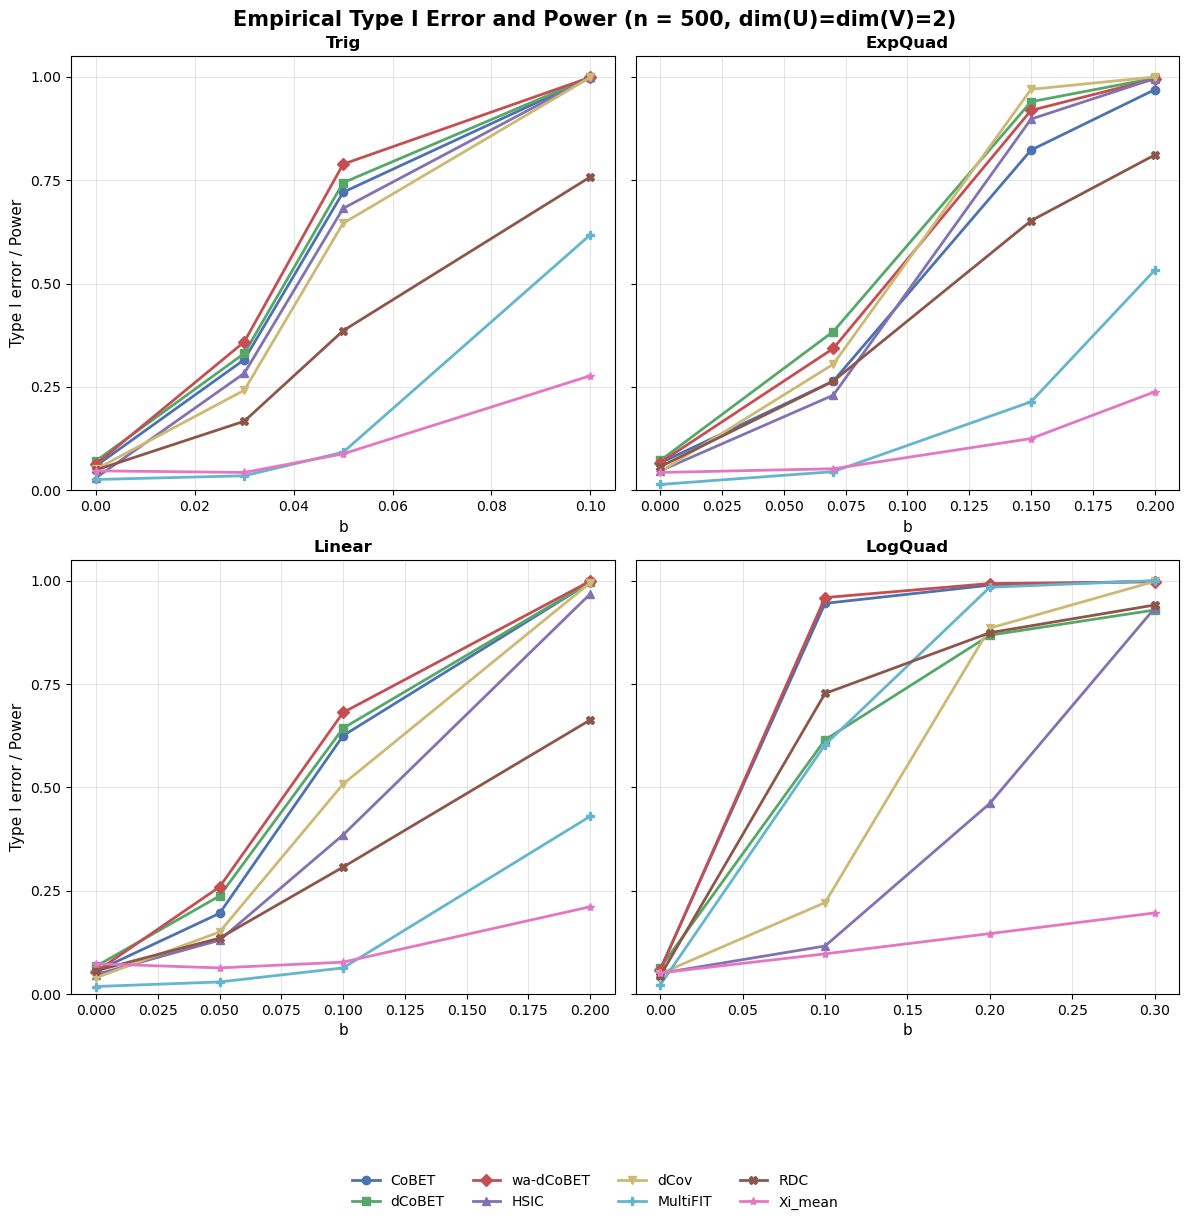
\includegraphics[
            width=\linewidth,
            height=0.48\textheight,
            keepaspectratio,
            alt={Empirical size and power curves for CoBET, dCoBET,
            wa-dCoBET, HSIC, dCov, RDC, Xi-mean, and MultiFIT under
            four dependence structures with sample size 500 and
            dimensions of U and V equal to 2.}
        ]{plots/dim2_n500.png}
        \caption{$\dim(U)=\dim(V)=2$.}
    \end{subfigure}
    \hfill
    \begin{subfigure}[t]{0.48\textwidth}
        \centering
        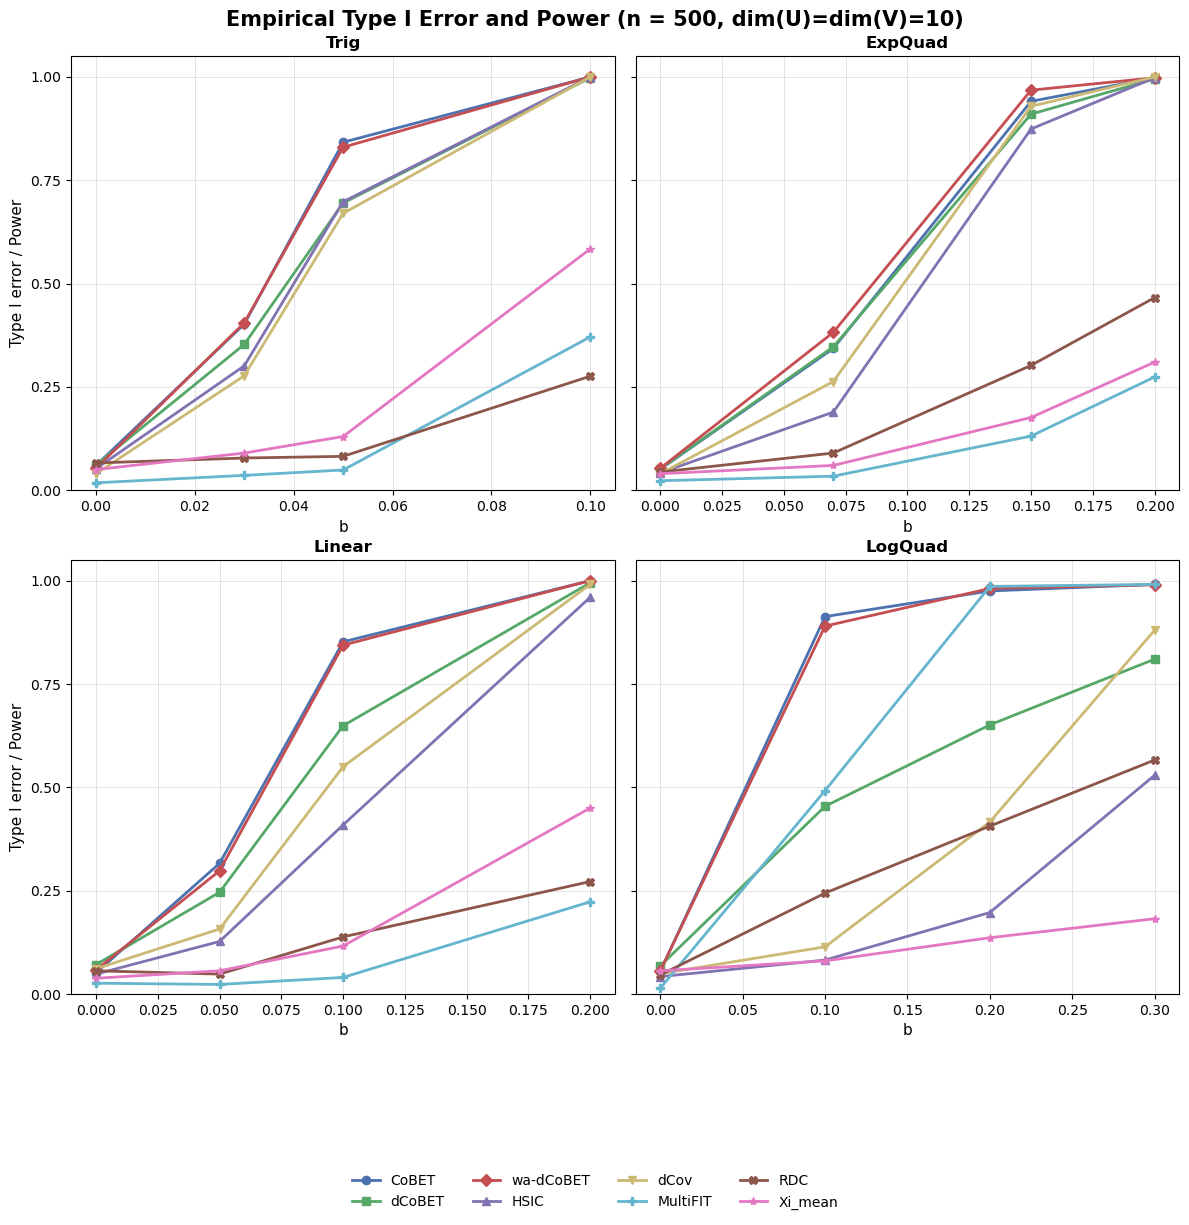
\includegraphics[
            width=\linewidth,
            height=0.48\textheight,
            keepaspectratio,
            alt={Empirical size and power curves for CoBET, dCoBET,
            wa-dCoBET, HSIC, dCov, RDC, Xi-mean, and MultiFIT under
            four dependence structures with sample size 500 and
            dimensions of U and V equal to 10.}
        ]{plots/dim10_n500.png}
        \caption{$\dim(U)=\dim(V)=10$.}
    \end{subfigure}

    \caption{Empirical size and power comparison of CoBET, dCoBET,
    wa-dCoBET, HSIC, dCov, RDC, Xi-mean, and MultiFIT as a function
    of signal strength $b$ for sample size $n=500$. Results are shown
    for four dependence structures under low- and higher-dimensional
    settings.}
    \label{fig:power-n500}
\end{figure}


% ============================================================
% Empirical Size and Power: n = 250
% ============================================================

\begin{figure}[htbp]
    \centering

    \begin{subfigure}[t]{0.48\textwidth}
        \centering
        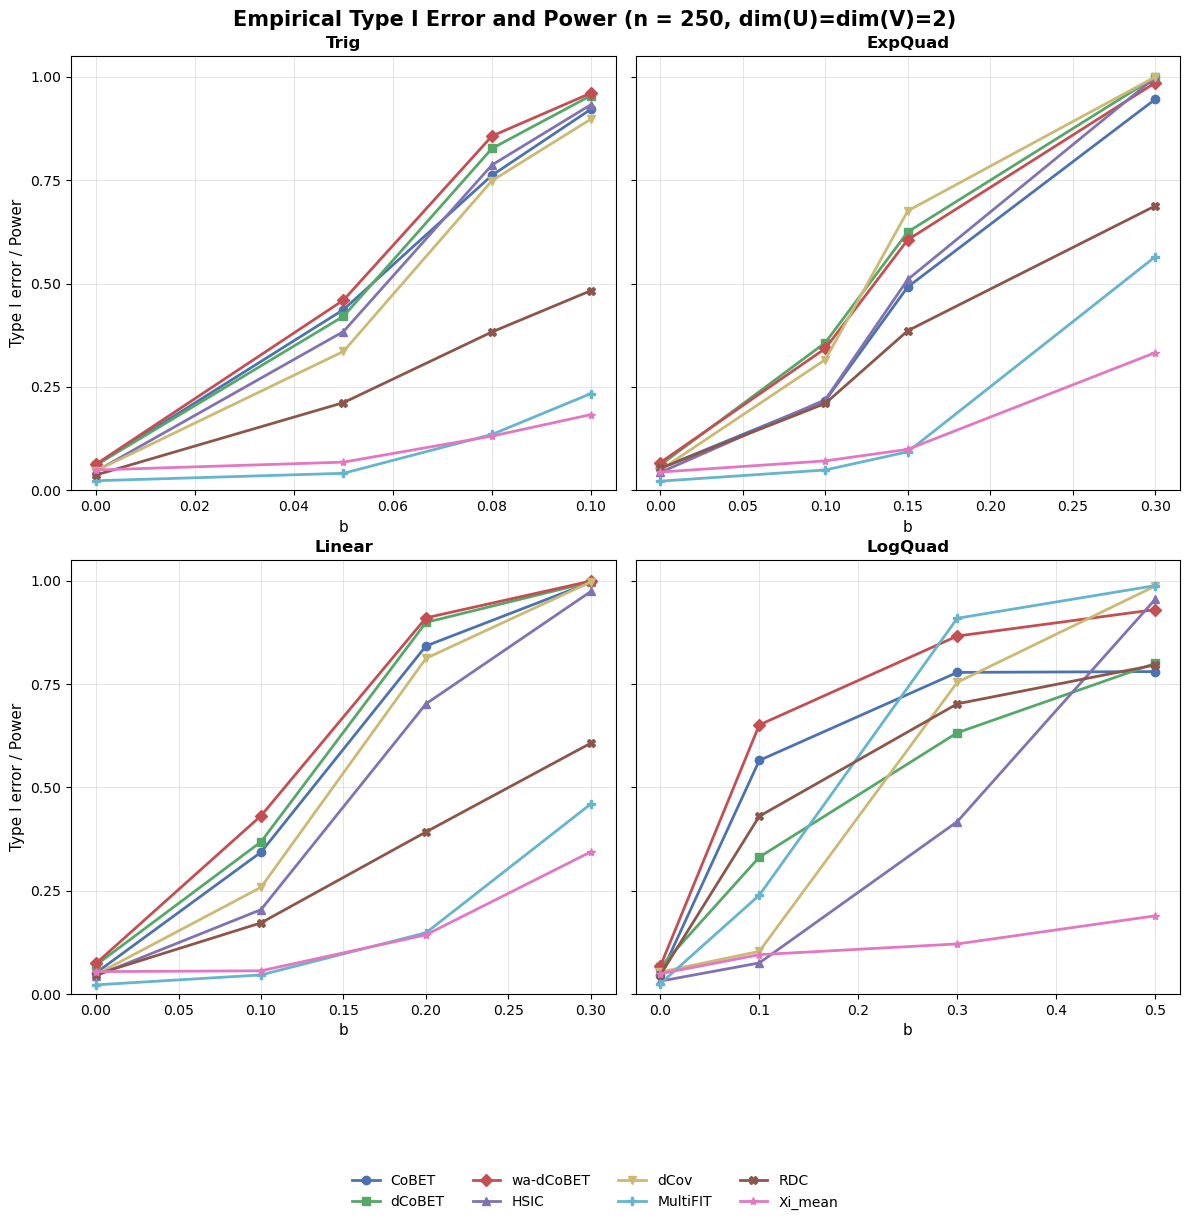
\includegraphics[
            width=\linewidth,
            height=0.48\textheight,
            keepaspectratio,
            alt={Empirical size and power curves for CoBET, dCoBET,
            wa-dCoBET, HSIC, dCov, RDC, Xi-mean, and MultiFIT under
            four dependence structures with sample size 250 and
            dimensions of U and V equal to 2.}
        ]{plots/dim2_n250.png}
        \caption{$\dim(U)=\dim(V)=2$.}
    \end{subfigure}
    \hfill
    \begin{subfigure}[t]{0.48\textwidth}
        \centering
        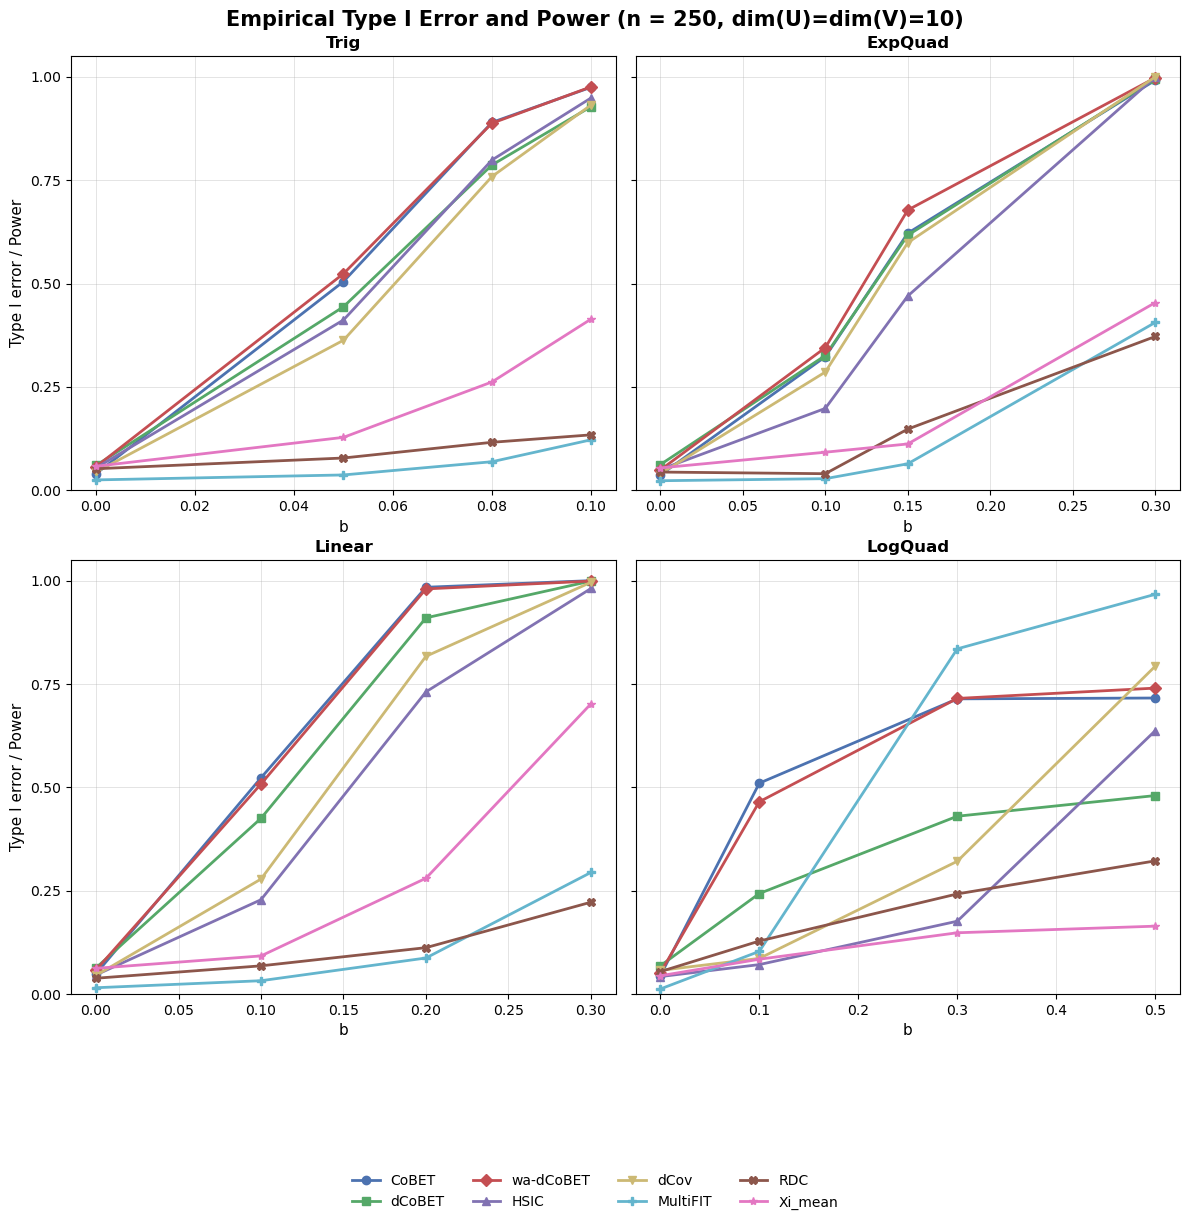
\includegraphics[
            width=\linewidth,
            height=0.48\textheight,
            keepaspectratio,
            alt={Empirical size and power curves for CoBET, dCoBET,
            wa-dCoBET, HSIC, dCov, RDC, Xi-mean, and MultiFIT under
            four dependence structures with sample size 250 and
            dimensions of U and V equal to 10.}
        ]{plots/dim10_n250.png}
        \caption{$\dim(U)=\dim(V)=10$.}
    \end{subfigure}

    \caption{Empirical size and power comparison of CoBET, dCoBET,
    wa-dCoBET, HSIC, dCov, RDC, Xi-mean, and MultiFIT as a function
    of signal strength $b$ for sample size $n=250$. Results are shown
    for four dependence structures under low- and higher-dimensional
    settings. Results correspond to the same dependence structures
    and testing procedures as in Figure~\ref{fig:power-n500}.}
    \label{fig:power-n250}
\end{figure}


% ============================================================
% Empirical Size and Power: n = 1000
% ============================================================

\begin{figure}[htbp]
    \centering

    \begin{subfigure}[t]{0.48\textwidth}
        \centering
        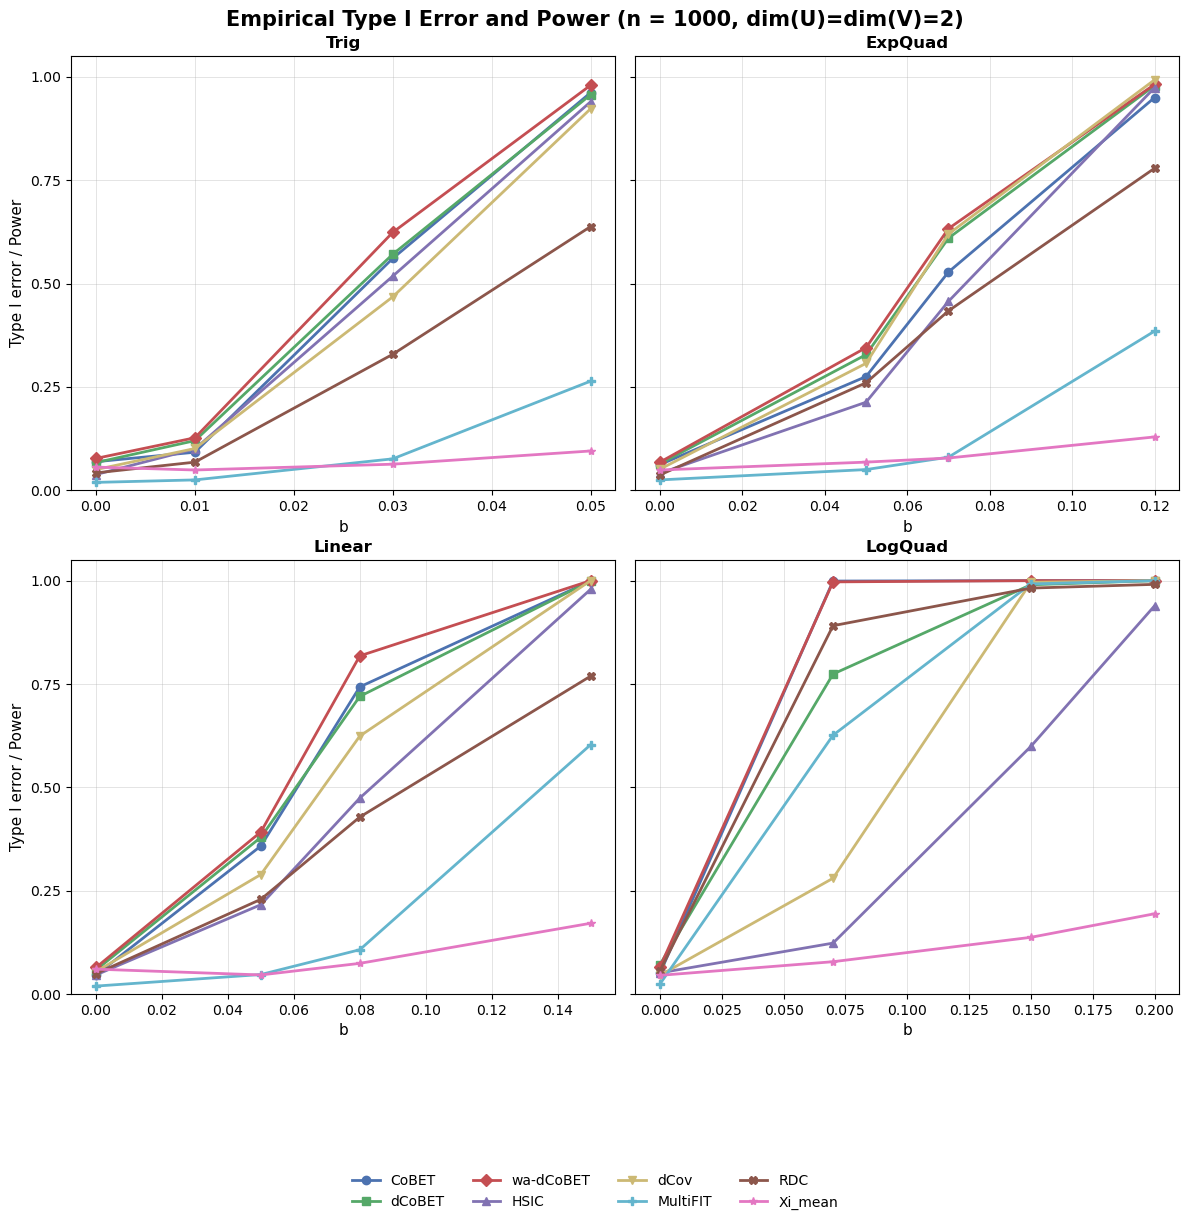
\includegraphics[
            width=\linewidth,
            height=0.48\textheight,
            keepaspectratio,
            alt={Empirical size and power curves for CoBET, dCoBET,
            wa-dCoBET, HSIC, dCov, RDC, Xi-mean, and MultiFIT under
            four dependence structures with sample size 1000 and
            dimensions of U and V equal to 2.}
        ]{plots/dim2_n1000.png}
        \caption{$\dim(U)=\dim(V)=2$.}
    \end{subfigure}
    \hfill
    \begin{subfigure}[t]{0.48\textwidth}
        \centering
        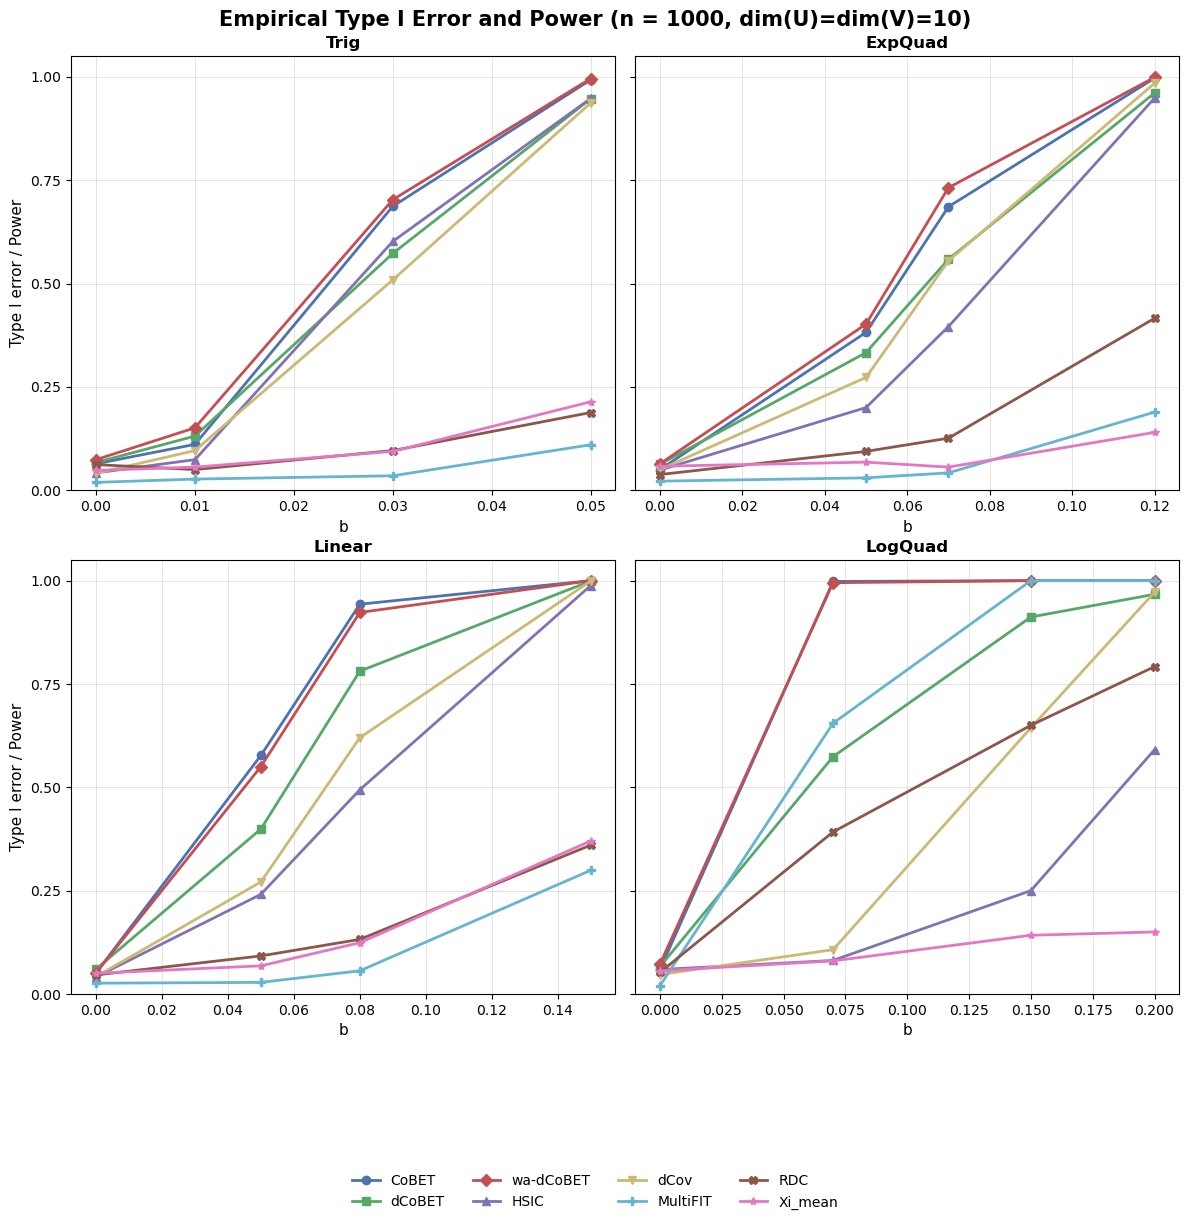
\includegraphics[
            width=\linewidth,
            height=0.48\textheight,
            keepaspectratio,
            alt={Empirical size and power curves for CoBET, dCoBET,
            wa-dCoBET, HSIC, dCov, RDC, Xi-mean, and MultiFIT under
            four dependence structures with sample size 1000 and
            dimensions of U and V equal to 10.}
        ]{plots/dim10_n1000.png}
        \caption{$\dim(U)=\dim(V)=10$.}
    \end{subfigure}

    \caption{Empirical size and power comparison of CoBET, dCoBET,
    wa-dCoBET, HSIC, dCov, RDC, Xi-mean, and MultiFIT as a function
    of signal strength $b$ for sample size $n=1000$. Results are shown
    for four dependence structures under low- and higher-dimensional
    settings. Results correspond to the same dependence structures
    and testing procedures as in Figure~\ref{fig:power-n500}.}
    \label{fig:power-n1000}
\end{figure}

% In the higher-dimensional setting ($d=10$), the contrast between methods becomes
% more pronounced. While all procedures eventually attain high power for Trig,
% ExpQuad, and Linear alternatives as $b$ increases, wa-dCoBET systematically
% exhibits earlier detection and steeper power curves. HSIC methods
% generally require stronger signals to reach comparable power, suggesting their sensitivity to dimensionality.

% The LogQuad case presents the most challenging scenario. Here, HSIC and dCov
% are less powerful in higher dimension at moderate signal levels.
% In contrast, wa-dCoBET maintains strong performance across the entire signal
% range and approaches unit power at values of $b$ where competing methods remain far from saturation. These results demonstrate the robustness of adaptive binary expansion in detecting complex, higher-dimensional dependence.
Figures~\ref{fig:power-n250} and~\ref{fig:power-n1000} show consistent patterns:
CoBET, dCoBET, and wa-dCoBET remain strongest, RDC is competitive mainly in low
dimension, MultiFIT is effective primarily for LogQuad, and Xi-mean is generally
the weakest.

\paragraph{Pairwise heatmap diagnostics.}
To visualize coordinate-level dependence, we report heatmaps of pairwise
standardized test statistics. Each cell corresponds to the $Z$-statistic for
testing dependence between a coordinate of $X$ and a coordinate of $Y$, with
darker colors indicating stronger evidence against independence. Multiple
testing across coordinate pairs is controlled using the
Benjamini--Hochberg false discovery rate (FDR) procedure
\cite{benjamini1995controlling}; significant pairs are displayed with higher
opacity.

Figure~\ref{fig:logquad_three_cases} illustrates three representative scenarios
under the LogQuad transformation with $d=10$. When $(\theta,b)=(0,0)$, the
heatmap shows no significant entries. When $(\theta,b)=(0,0.4)$, dependence is
restricted to matched coordinates, producing a clear diagonal pattern. When
$(\theta,b)=(2,0.4)$, dependence arises from the copula structure, yielding
additional off-diagonal discoveries. These cases demonstrate how the heatmap
distinguishes null behavior, sparse coordinate-wise dependence, and broader
multivariate dependence.


\begin{figure}[!t]
    \centering

    % Null case: theta = 0, b = 0
    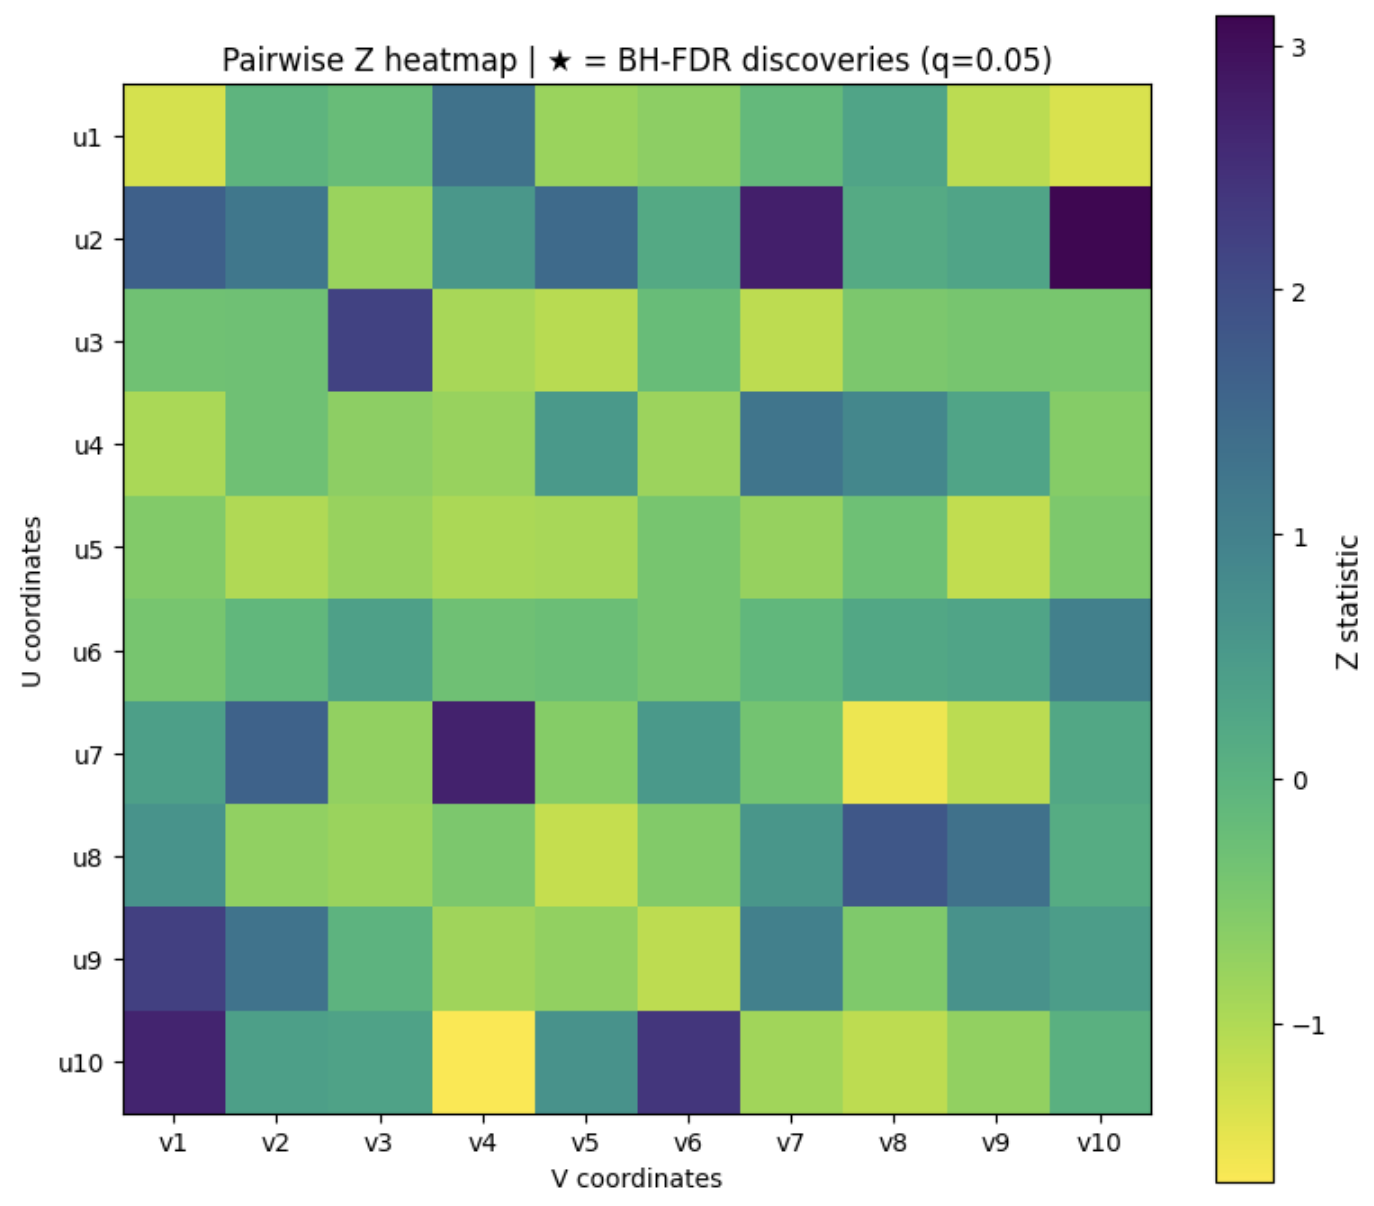
\includegraphics[
      trim=14pt 12pt 14pt 12pt,
      clip,
      width=0.34\columnwidth,
      height=0.2\textheight,
      keepaspectratio,
      alt={Pairwise Z-statistic heatmap for the LogQuad model with
      dimension 10, theta equal to 0, and b equal to 0. The heatmap
      represents the null setting with no systematic pairwise
      dependence pattern.}
    ]{plots/independent.png}
    \hspace{-0.6em}%
    %
    % Dependent case: theta = 0, b = 0.4
    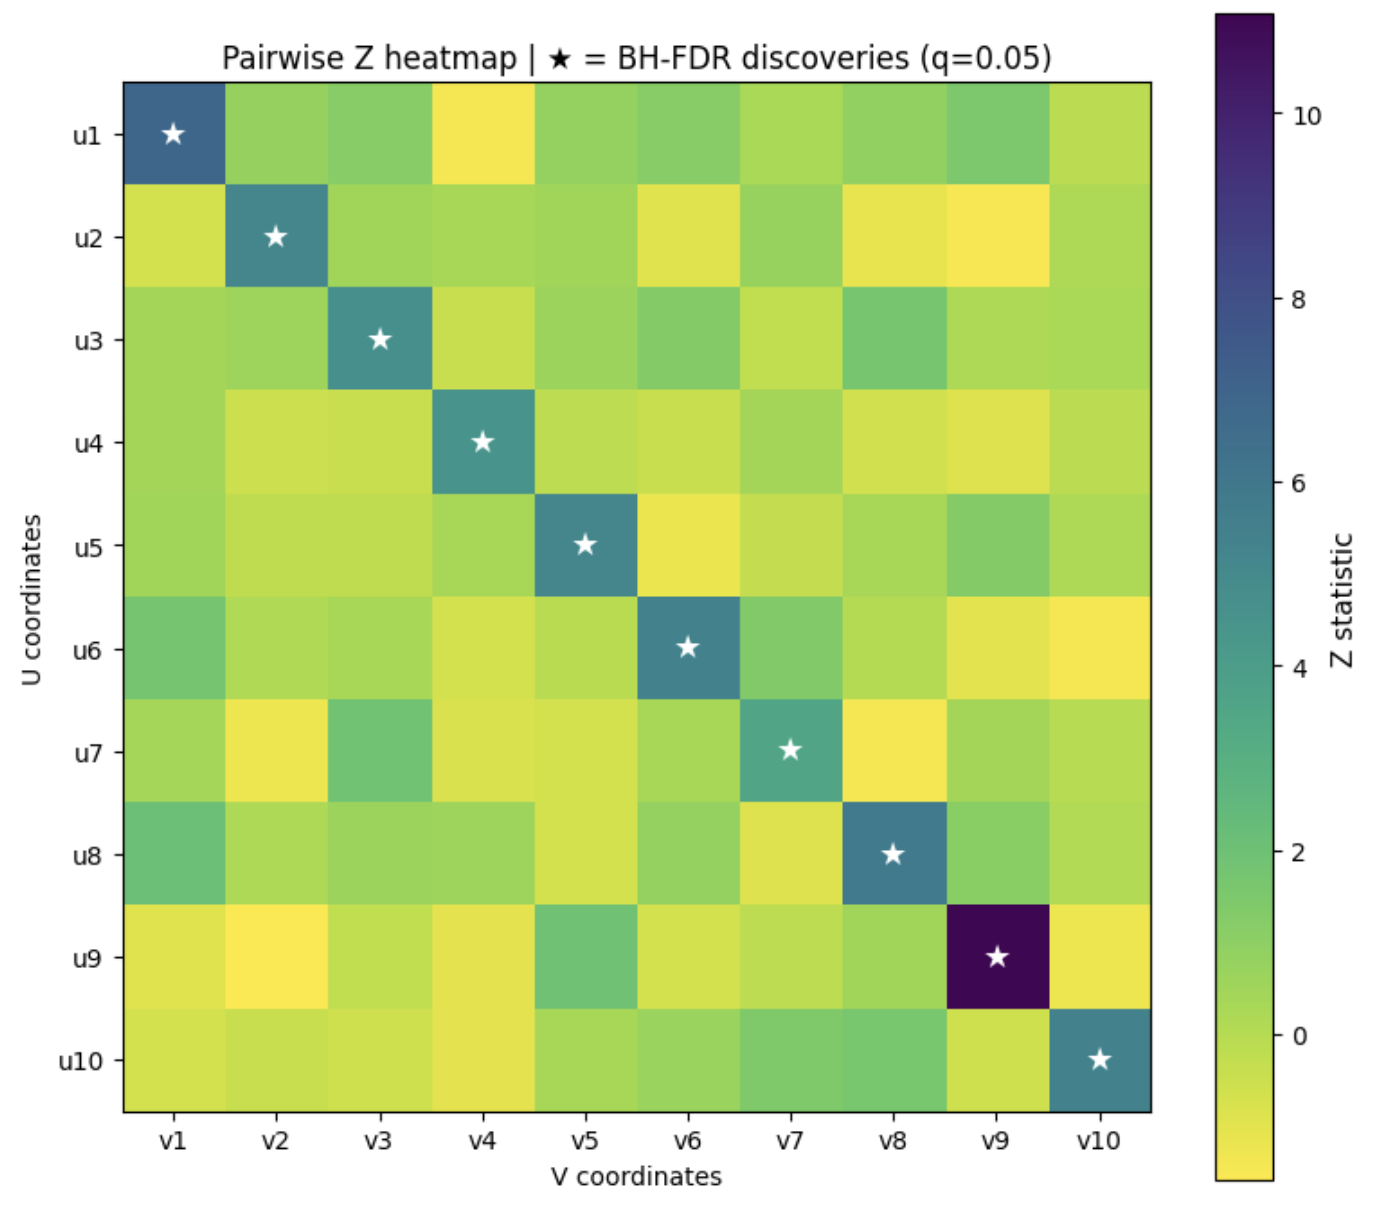
\includegraphics[
      trim=14pt 12pt 14pt 12pt,
      clip,
      width=0.34\columnwidth,
      height=0.2\textheight,
      keepaspectratio,
      alt={Pairwise Z-statistic heatmap for the LogQuad model with
      dimension 10, theta equal to 0, and b equal to 0.4. The heatmap
      shows stronger dependence concentrated primarily along matched
      coordinate pairs, producing a diagonal pattern.}
    ]{plots/dependent1.png}
    \hspace{-0.6em}%
    %
    % Dependent case: theta = 2, b = 0.4
    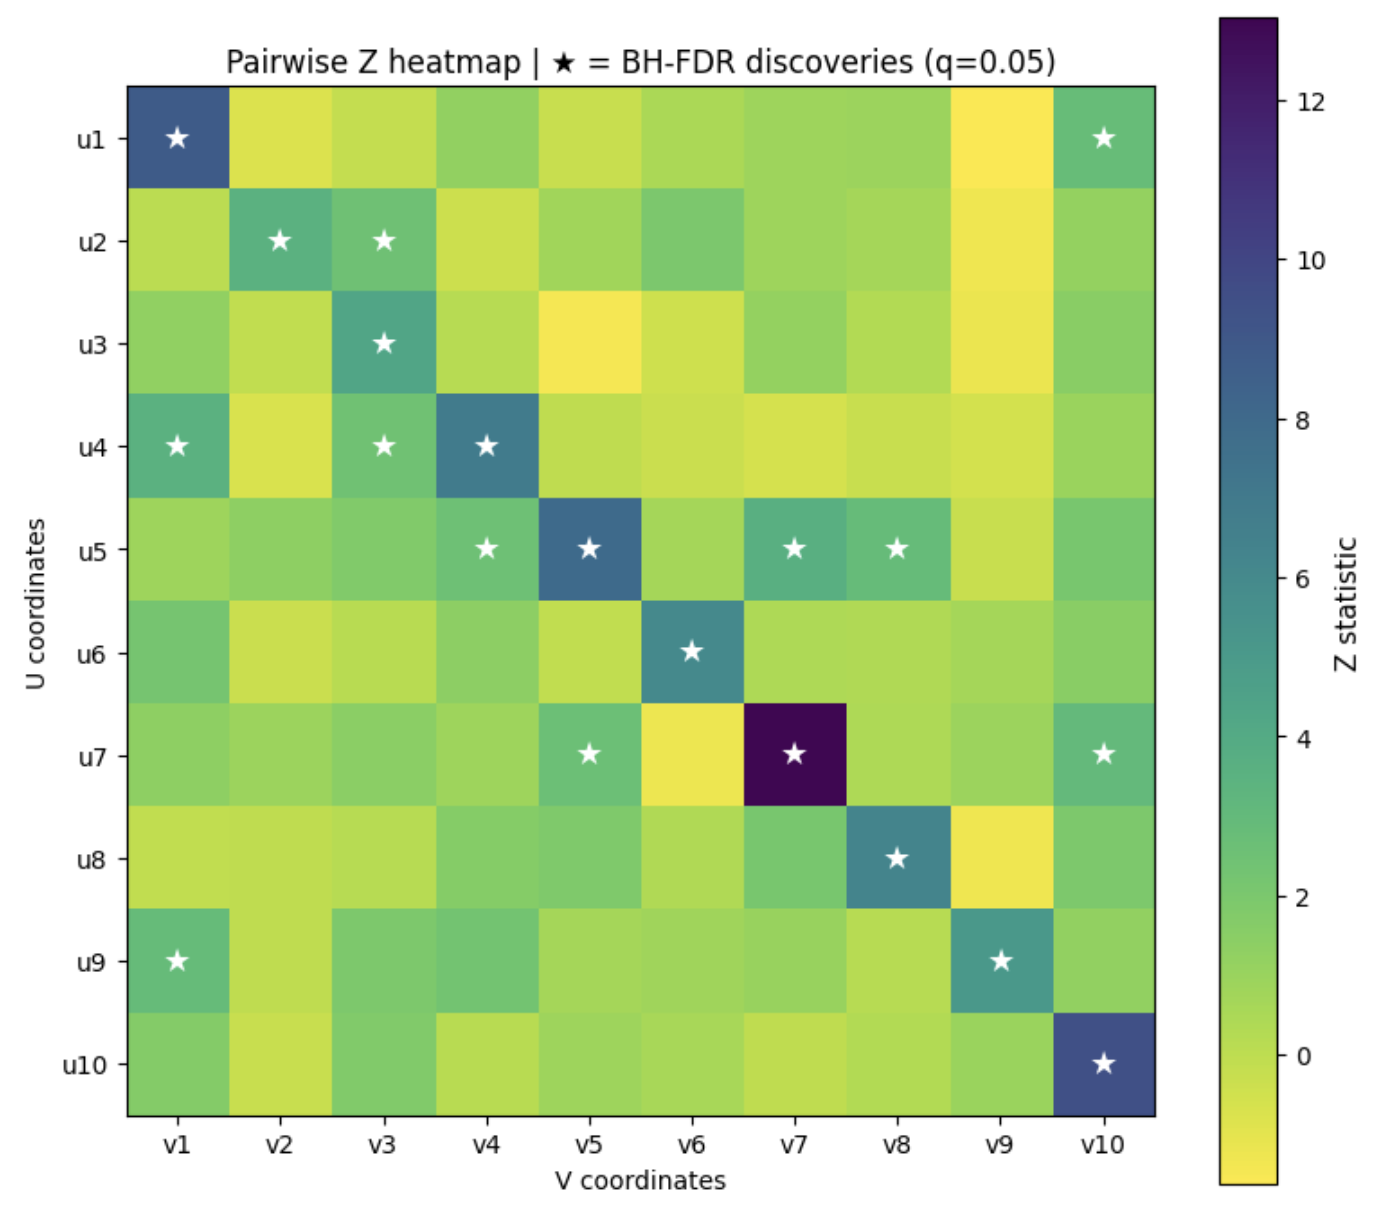
\includegraphics[
      trim=14pt 12pt 14pt 12pt,
      clip,
      width=0.34\columnwidth,
      height=0.2\textheight,
      keepaspectratio,
      alt={Pairwise Z-statistic heatmap for the LogQuad model with
      dimension 10, theta equal to 2, and b equal to 0.4. The heatmap
      shows dependence along matched coordinates together with
      additional off-diagonal dependence between coordinate pairs.}
    ]{plots/dependent2.png}

    \caption{\scriptsize
    Pairwise $Z_n$--statistic heatmaps for the LogQuad model with
    $d=10$. Left: $\theta=0,b=0$; middle: $\theta=0,b=0.4$;
    right: $\theta=2,b=0.4$. Larger $Z_n$ values indicate stronger
    pairwise dependence detected by the proposed statistic; the
    middle panel exhibits primarily diagonal dependence, while the
    right panel additionally exhibits off-diagonal dependence.
    }
    \label{fig:logquad_three_cases}

    \vspace{-0.7em}
\end{figure}


\subsection{Adaptive Weighting Behavior under Log-Quadratic Dependence}

We provide results to further illustrate the behavior of the proposed adaptive weighting mechanism under complex nonlinear dependence. The proposed framework captures high-order interactions through the choice of resolution level $K$, while the SNR-based voting scheme adaptively selects weight matrices that enhance detection power.

We consider the logquad setting described in Section~3.1, which is among the most difficult scenarios due to its combination of oscillatory behavior and localized signal structure. Such dependence cannot be effectively captured by a single interaction scale and instead requires aggregating information across multiple orders. In this setting, we fix $p=q=10$, vary the sample size $n \in \{250,500,1000\}$, and evaluate performance over $R=500$ replications at significance level $\alpha=0.05$.

The results in Table~\ref{tab:logquad_weight_power_compare} show that the proposed wa-dCoBET consistently achieves power comparable to or exceeding CoBET while substantially outperforming dCoBET across all signal levels. 

The adaptive combination provides a clear advantage by learning weights in a data-driven approach. The learned weights reflect 
the relative detection powers between CoBET and dCoBET as the sample size and signal strength vary, which consistently assigns higher weights to the test with higher power. At the same time, all methods maintain controlled Type I error. Together, these results provide direct empirical evidence that the proposed adaptive weighting mechanism effectively captures complex dependence structures by dynamically balancing contributions from different interaction orders.

\begin{table}[ht]
\centering
\begin{tabular}{ccccccc}
\hline
$n$ & $b$ & CoBET & dCoBET & wa-dCoBET & Avg $\hat{w}_{\mathrm{id}}$ & Avg $\hat{w}_D$ \\
\hline
\multicolumn{7}{c}{\textbf{Sample size $n=250$}} \\
\hline
250 & 0.00 & 0.045 & 0.065 & 0.051 & 0.5951 & 0.4049 \\
250 & 0.10 & 0.510 & 0.243 & 0.465 & 0.5793 & 0.4207 \\
250 & 0.30 & 0.714 & 0.430 & 0.715 & 0.5555 & 0.4445 \\
250 & 0.50 & 0.716 & 0.480 & 0.720 & 0.5640 & 0.4360 \\
\hline
\multicolumn{7}{c}{\textbf{Sample size $n=500$}} \\
\hline
500 & 0.00 & 0.055 & 0.068 & 0.056 & 0.5629 & 0.4371 \\
500 & 0.10 & 0.913 & 0.454 & 0.890 & 0.5898 & 0.4102 \\
500 & 0.20 & 0.975 & 0.651 & 0.981 & 0.5541 & 0.4459 \\
500 & 0.30 & 0.991 & 0.760 & 0.989 & 0.5528 & 0.4472 \\
\hline
\multicolumn{7}{c}{\textbf{Sample size $n=1000$}} \\
\hline
1000 & 0.00 & 0.059 & 0.066 & 0.072 & 0.5459 & 0.4541 \\
1000 & 0.07 & 0.998 & 0.574 & 0.995 & 0.6383 & 0.3617 \\
1000 & 0.15 & 1.000 & 0.912 & 1.000 & 0.6266 & 0.3734 \\
1000 & 0.20 & 1.000 & 0.967 & 1.000 & 0.5986 & 0.4014 \\
\hline
\end{tabular}
\caption{Power comparison of CoBET, dCoBET, and wa-dCoBET, together with the average adaptive weights under the logquad setting ($d=10$, $R=500$, $\alpha=0.05$).}
\label{tab:logquad_weight_power_compare}
\end{table}

\subsection{Cross-Dimensional Nonlinear Dependence}

To evaluate performance of the proposed methods under more complex dependence structures, we conducted additional simulations involving \emph{cross-dimensional interactions} and \emph{non-separable nonlinear dependence}.

Specifically, we consider a multivariate setting with $X, Y \in \mathbb{R}^d$ ($d=10$), where the dependence between $X$ and $Y$ is driven by interactions across multiple coordinates of $X$. Let $X$ be generated from a nonlinear transformation of a multivariate copula-based sample similar to the generation $X$ in Section 3.1. The random vector $Y=(Y_1,\cdots,Y_d)^\prime$ is generated by the following model:
\begin{equation}
Y_j = \cos\!\bigl( b \cdot (X_1 X_2 + X_3 X_4) + V \bigr)
\cdot \exp\!\bigl( -b (X_5 - 0.5)^2 \bigr)
+ \varepsilon_j, 
\quad j = 1,\dots,d,
\end{equation}
where $V \sim \mathrm{Unif}(0,1)$ and $\varepsilon_j \sim \mathcal{N}(0, \sigma^2)$ are independent noise terms.
This data generation introduces several dependence and challenges:
(i) multiplicative cross-dimensional interactions (e.g., $X_1 X_2$),
(ii) non-additive nonlinear structure,
and (iii) a shared latent signal across coordinates of $Y$ through $V$.
Such dependence cannot be decomposed into coordinate-wise relationships and therefore provides a setting to evaluate the proposed method's ability to detect complex joint dependence.

We evaluate the proposed methods with sample size $n=500$, dimension $d=10$, resolution $K=4$, and simulation replication $R=500$ replications. The parameter $b$ controls the signal strength, where $b=0$ corresponds to the null hypothesis of independence.

\begin{table}[ht]
\centering
\begin{tabular}{cccccccccc}
\hline
$b$ & CoBET & dCoBET & wa-dCoBET & $\mbox{Avg}\; \hat{w}_{\text{id}}$ & $\mbox{Avg}\;\hat{w}_{D}$ \\
\hline
 0.0 & 0.044 & 0.072 & 0.058 & 0.540 & 0.460 \\
 0.1 & 0.076 & 0.092 & 0.11 & 0.457 & 0.543 \\
 0.2 & 0.200 & 0.236 & 0.278 & 0.478 & 0.522 \\
 0.3 & 0.510 & 0.570 & 0.602 & 0.494 & 0.506 \\
 0.5 & 0.952 & 0.970 & 0.982 & 0.392 & 0.608 \\
\hline
\end{tabular}
\caption{Empirical Type I error and power under cross-dimensional nonlinear dependence.}
\end{table}

The results demonstrate that CoBET, dCoBET and wa-dCoBET maintain valid Type I error under the null ($b=0$), with wa-dCoBET remaining well-calibrated. Under increasing signal strength, all methods exhibit increasing power, confirming their ability to detect cross-dimensional complex dependence.

\subsection{Comparison with BET \cite{zhang2019bet} in the Univariate Dimension Setting}

Testing independence between one-dimensional random variable, both the proposed method and Zhang's max BET \cite{zhang2019bet} statistic are applicable. Since Zhang's BET \cite{zhang2019bet} is based on the maximum norm and measures the symmetric in binary interactions, BET is more powerful when the strong dependence exists in sparse binary interactions while the proposed test is more powerful when the weak dependence exist in dense (many) binary interactions. 
    
However, it is important to note that BET \cite{zhang2019bet} is not applicable to higher-dimensional case due to the computational burden since it requires to obtain the entire vector of binary expansion interactions, which grows exponentially fast as data dimension and resolution grow. The proposed method overcomes this issue by introducing the kernel representations.

To examine the relative performance of the proposed aggregation-based and max-type independence tests \cite{zhang2019bet}, we consider the \texttt{logquad} setting introduced in Section~3.1 with $p=q=1$. The dependence strength is controlled by the parameter $b$, where $b=0$ corresponds to the null hypothesis and $b>0$ introduces increasing levels of nonlinear dependence. Based on the construction, all the binary interaction coefficients are non-zero in the dependence between $X$ and $Y$, which is the dense regime. 

We compare the proposed CoBET, dCoBET, wa-dCoBET, with Zhang's Max BET \cite{zhang2019bet} by setting the sample size at $n=500$ and the significance level $\alpha=0.05$. The binary expansion depth is set to $K=4$. The results are summarized in Table 3.
\begin{table}[ht]
\centering
\label{tab:dense_bet_comparison}
\begin{tabular}{ccccccccc}
\hline
 $b$ & CoBET & dCoBET & wa-dCoBET & BET \\
\hline
 0.0 & 0.048 & 0.068 & 0.058 & 0.036 \\
 0.1 & 0.926 & 0.678 & 0.948 & 0.494  \\
 0.2 & 0.990 & 0.892 & 0.996 & 0.864  \\
 0.3 & 0.998 & 0.942 & 0.998 & 0.978  \\
 0.5 & 1.000 & 0.916 & 1.000 & 0.998  \\
\hline
\end{tabular}
\caption{Empirical size and power for the proposed tests and their comparison with BET \cite{zhang2019bet}.}
\end{table}
The results clearly illustrate the trade-off between aggregation-based and max-type statistics. Under the null hypothesis ($b=0$), all methods maintain valid Type I error. Under dense alternatives, however, substantial differences emerge.

In the weak-signal regime ($b=0.1$), Max BET achieves only $0.494$ power, while wa-dCoBET reaches $0.948$, nearly doubling the detection rate. This gap highlights the well-known limitation of max-type statistics: when the signal is distributed across many components rather than concentrated in a single dominant interaction, the maximum statistic fails to accumulate evidence effectively. In contrast, wa-dCoBET aggregates information across all binary expansion coefficients through a quadratic form, enabling it to capture distributed weak signals. As the signal strength increases, the performance gap narrows, and all methods approach full power. Overall, the experiments provide empirical evidence that wa-dCoBET outperforms Max BET in dense signal regimes.


\subsection{ Choosing the Binary Expansion Resolution $K$}
\label{choose_k}
 The resolution hyperparameter $K$ may be selected in a data-driven manor by maximizing the SNR of the power function in practice. Theoretically speaking, the computational complexity of the proposed test is linear in the depth (resolution) $K$. The asymptotic power of the test is determined by the SNR estimated
in the algorithm. To choose an appropriate $K$, one could find $K$ that maximizes the SNR of the test while choosing $K$ in 
reasonable range.

To provide practical guidance on the choice of the binary expansion depth $K$ and investigate the trade-off between power and computational efficiency, we conducted an additional sensitivity analysis of wa-dCoBET using the logquad function used simulation study (section 3.1), which is among the most challenging dependence settings considered. 


In this experiment, the sample size was $n=500$, and both $X$ and $Y$ were $10$-dimensional vectors ($p=q=10$). We evaluated several values of the binary expansion depth $K$ in the range $K \in \{3,4,5,6\}$. For each $K$, we examined both type~I error under the null and power under the logquad alternative with signal strength $b=0.3$. The results are summarized in Table \ref{tab:K_sensitivity_wa_dcobet}. We observe that the results were generally stable across this range. In particular, the empirical type~I error remained close to the nominal $0.05$ level, while power remained high for all four choices of $K$. At the same time, the computational cost increased substantially with $K$, reflecting the exponential growth in the number of interaction terms.

 These results illustrate the practical trade-off governed by $K$. Larger values of $K$ increase the resolution of the binary expansion and can capture more complex dependence structures, but they also lead to higher variance and more computational cost. Smaller values are more computational efficient, but may be less sensitive to finer-scale nonlinear dependent patterns. In our experiment, $K=4$ achieved essentially maximal power while maintaining near-nominal type~I error and substantially lower runtime than $K=5$ or $K=6$. Based on these considerations, we recommend selecting $K$ in a moderate range (e.g., $K=3$--$6$) and checking robustness across nearby values, with $K=4$ serving as a practical default for moderate sample sizes and dimensions.

\begin{table}[htbp!]
\centering
\begin{tabular}{c c c c}
\hline
$K$ & Type I error & Power ($b=0.3$) & Runtime (sec) \\
\hline
3 & 0.064 & 0.98 & 0.026863 \\
4 & 0.070 & 1.00 & 0.048775 \\
5 & 0.052 & 0.97 & 0.165217 \\
6 & 0.042 & 0.94 & 1.051935 \\
\hline
\end{tabular}
\caption{Sensitivity of wa-dCoBET to the binary expansion depth $K$ under the logquad setting. Reported are the empirical type~I error, empirical power for the alternative with $b=0.3$, and the average runtime (in seconds).}
\label{tab:K_sensitivity_wa_dcobet}
\end{table}

To evaluate computational scalability with respect to data dimension and resolution, we conducted a systematic study under the logquad function which is simulation section 3.1 by varying the sample size $n \in \{500,1000,1500\}$, dimension $d \in \{10,30,50\}$, and binary expansion depth $K \in \{3,4,5,6\}$. The results are summarized in Table \ref{tab:computational_scaling}.

The empirical results show that the impact of dimension $d$ is relatively mild: increasing $d$ from 10 to 50 leads to only moderate increases in runtime, indicating that the kernel-style formulation avoids explicit enumeration of the exponentially large feature space. The expansion depth $K$ has slightly more impact on computational cost and the computational time is still reasonable. As $K$ increases, the runtime grows (e.g., from approximately 0.05 seconds at $K=3$ to about 2 seconds at $K=6$ when $n=500$, $d=50$).

Importantly, the method remains computationally efficient for moderate depths, where runtimes are well below one second even for larger sample sizes ($n=1500$) and higher dimensions ($d=50$). At the same time, statistical performance remains strong, with controlled Type I error and near-perfect power across all configurations.
Overall, these results indicate that the proposed method scales well in practice with respect to dimension, sample size, and the choice of $K$. 

\begin{table}[ht]
\centering
\small
\begin{tabular}{ccccccc}
\toprule
$n$ & $d$ & $K$ & Type I & Power($b=0.2)$ & Avg Runtime (sec) \\
\midrule
500  & 10 & 3 & 0.058 & 0.966 & 0.012 \\
500  & 30 & 3 & 0.070 & 0.928 & 0.031 \\
500  & 50 & 3 & 0.048 & 0.914 & 0.054 \\
1000 & 50 & 3 & 0.082 & 1.000 & 0.094 \\
1500 & 50 & 3 & 0.080 & 1.000 & 0.151 \\
\midrule
500  & 10 & 4 & 0.056 & 0.980 & 0.019 \\
500  & 50 & 4 & 0.050 & 0.934 & 0.136 \\
1000 & 50 & 4 & 0.074 & 1.000 & 0.213 \\
1500 & 50 & 4 & 0.072 & 1.000 & 0.312 \\
\midrule
500  & 10 & 5 & 0.048 & 0.966 & 0.031 \\
500  & 50 & 5 & 0.046 & 0.928 & 0.484 \\
1000 & 50 & 5 & 0.082 & 1.000 & 0.697 \\
1500 & 50 & 5 & 0.066 & 1.000 & 0.934 \\
\midrule
500  & 10 & 6 & 0.046 & 0.930 & 0.121 \\
500  & 50 & 6 & 0.024 & 0.890 & 2.379 \\
1000 & 50 & 6 & 0.088 & 1.000 & 3.666 \\
1500 & 50 & 6 & 0.054 & 1.000 & 3.994 \\
\bottomrule
\end{tabular}
\caption{Computational scaling of CoBET under the \texttt{logquad} setting. We vary sample size $n$, dimension $d$, and expansion depth $K$.}
\label{tab:computational_scaling}
\end{table}

\section{Real-World Application}
\label{sec:example}

We illustrate wa-dCoBET on corneal epithelial thickness data from a dry eye
disease study. The dataset contains measurements across 25 predefined corneal
regions for both eyes (OD and OS) from 189 subjects, obtained via anterior
segment optical coherence tomography. Each observation is represented as a
spatial thickness map, with regions corresponding to angular sectors and
concentric rings (See the left two in Figure~\ref{fig:realdata_application}).

\begin{figure}[!t]
    \centering
    \begin{subfigure}[b]{0.47\columnwidth}
        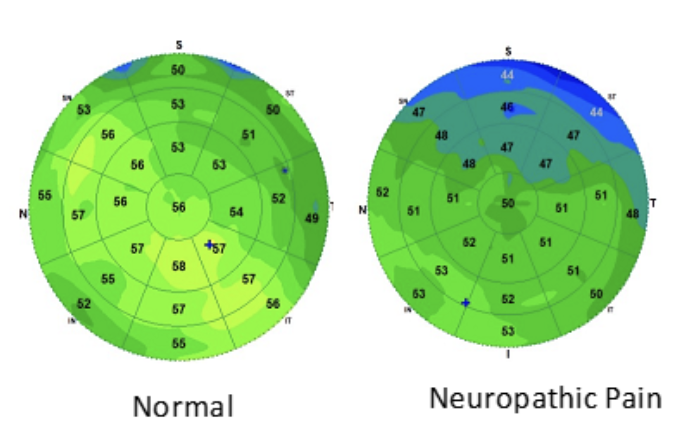
\includegraphics[
            width=\textwidth,
            height=0.22\textheight,
            keepaspectratio
        ]{plots/DED_1.png}
    \end{subfigure}
    \hspace{-0.1em}
    \begin{subfigure}[b]{0.47\columnwidth}
        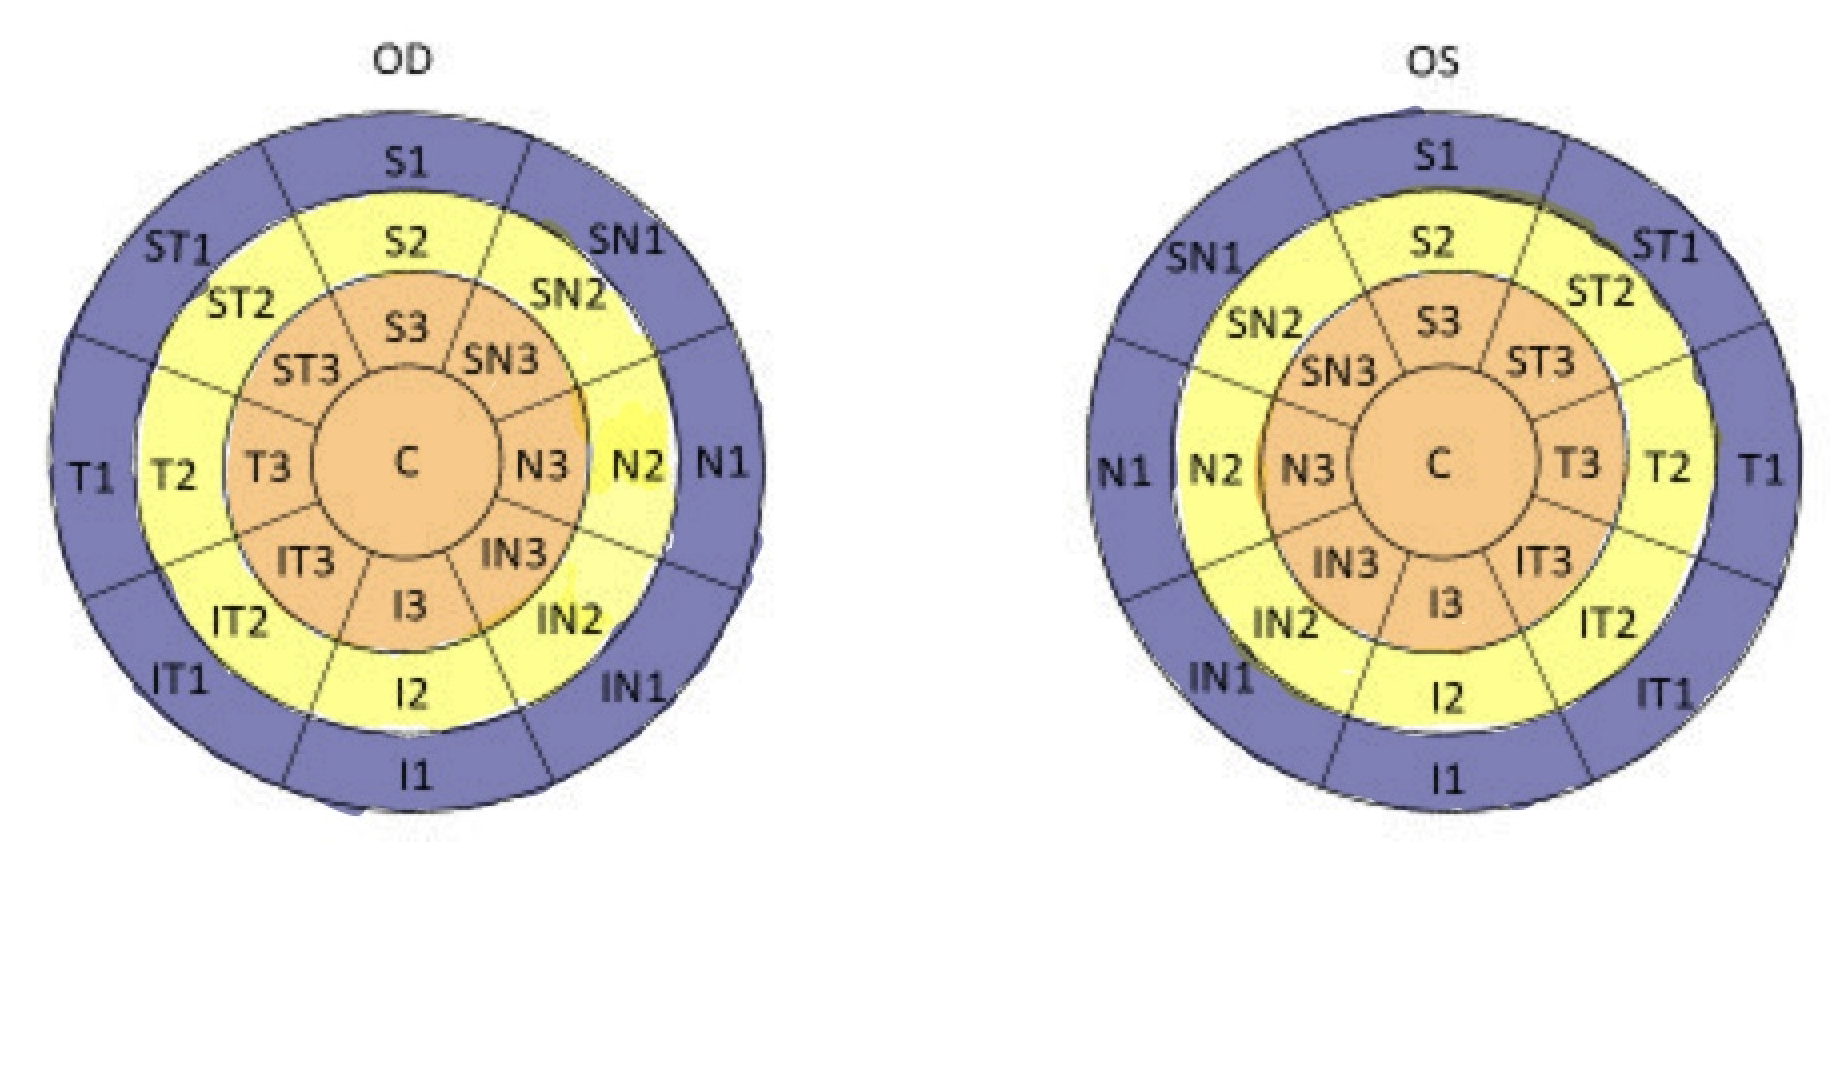
\includegraphics[
            width=\textwidth,
            height=0.22\textheight,
            keepaspectratio
        ]{plots/DED_example1.png}
    \end{subfigure}
    \caption{\scriptsize
    \textbf{Left:} Representative corneal epithelial thickness maps.
    Darker regions indicate thinner epithelium.
    \textbf{Right:} Regional partition used for dependence analysis.
    The cornea is divided into three concentric rings, with colors indicating different regions.
    }
    \label{fig:realdata_application}
    \vspace{-0.8em}
\end{figure}


\subsection{Regional dependence analysis via wa-dCoBET}
\label{sec:realdata_eye}

We apply wa-dCoBET to study dependence patterns in regional epithelial thickness,
focusing on %(i) dependence \emph{within} each eye across regions and 
dependence \emph{between} eyes across anatomically corresponding regions.
To balance geometric fidelity and dimensionality, the 25 regions are grouped
into three concentric sections and analyzed separately:
(i) central region plus inner ring ($p=q=10$),
(ii) middle ring ($p=q=8$), and
(iii) outer ring ($p=q=8$). See the right two in Figure \ref{fig:realdata_application} for an illustration.
For between-eye analysis, OD and OS vectors for each concentric sections are treated as $X$ and $Y$, respectively. For example, when $(X,Y)$ are, respectively, the OD and OS epithelial thickness for the central region plus inner ring, both $X, Y$ are 10-dimensional and hence $p=q=10$ for the central plus inner region. 

We first apply the proposed procedure to detect the dependence between two vectors $X$ and $Y$ for the three concentric sections defined above. The p-values for the three sections have shown significant dependence. To further interpret dependence, Figure~\ref{fig:eye_heatmaps_3sections} summarizes the inferred 
dependence structure. Across all three sections, wa-dCoBET detects 
strong \emph{between-eye} dependence, appearing as pronounced diagonal 
patterns that reflect tight correspondence between matched OD and OS 
regions.

Between-eye dependence exhibits a clear spatial gradient. In the central section,
strong off-diagonal signals indicate substantial mutual dependence among central
regions, consistent with a highly coherent epithelial structure near the visual
axis. This dependence weakens in the middle ring and is largely absent beyond
local neighborhoods in the outer ring, indicating increasing spatial
heterogeneity toward the periphery.

Overall, the analysis reveals a hierarchical organization of corneal epithelial
thickness: strong bilateral symmetry across all regions, coupled with
pronounced within-eye coherence in the central cornea that attenuates with
distance from the center. These findings highlight the ability of wa-dCoBET to
capture interpretable multiscale dependence patterns in structured biomedical data.

\begin{figure}[!t]
    \centering

    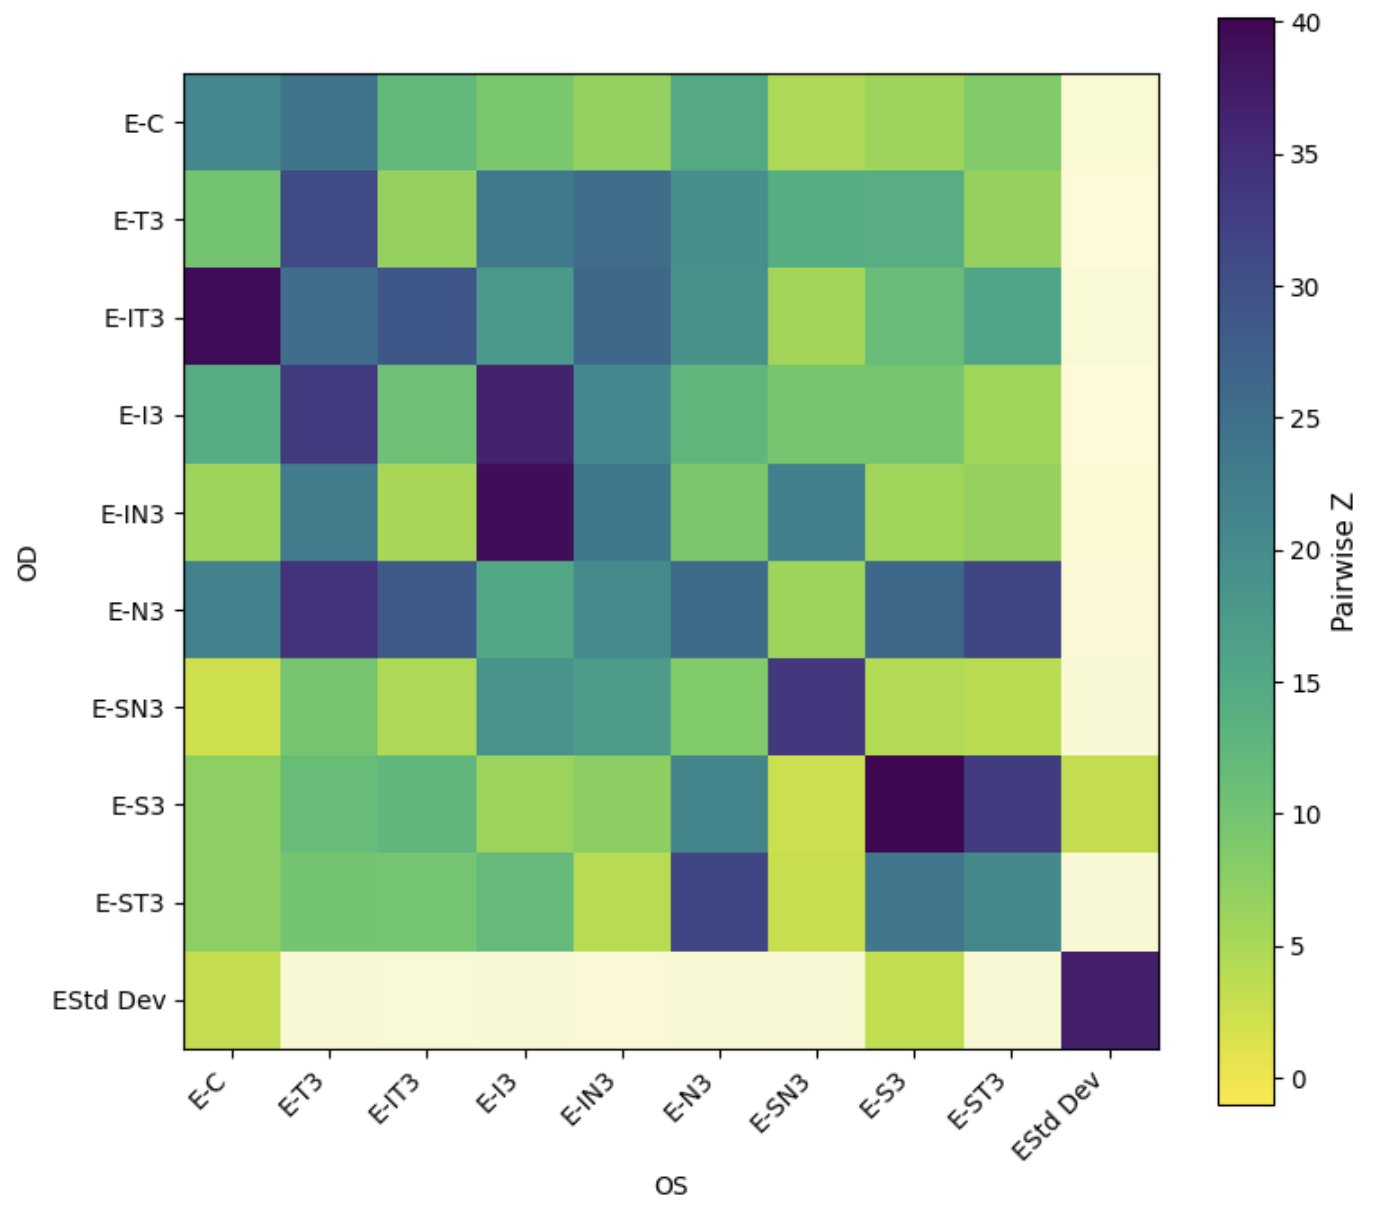
\includegraphics[
      trim=14pt 12pt 14pt 12pt,clip,
      width=0.34\columnwidth,height=0.2\textheight,keepaspectratio
    ]{plots/region_3.png}\hspace{-0.6em}%
    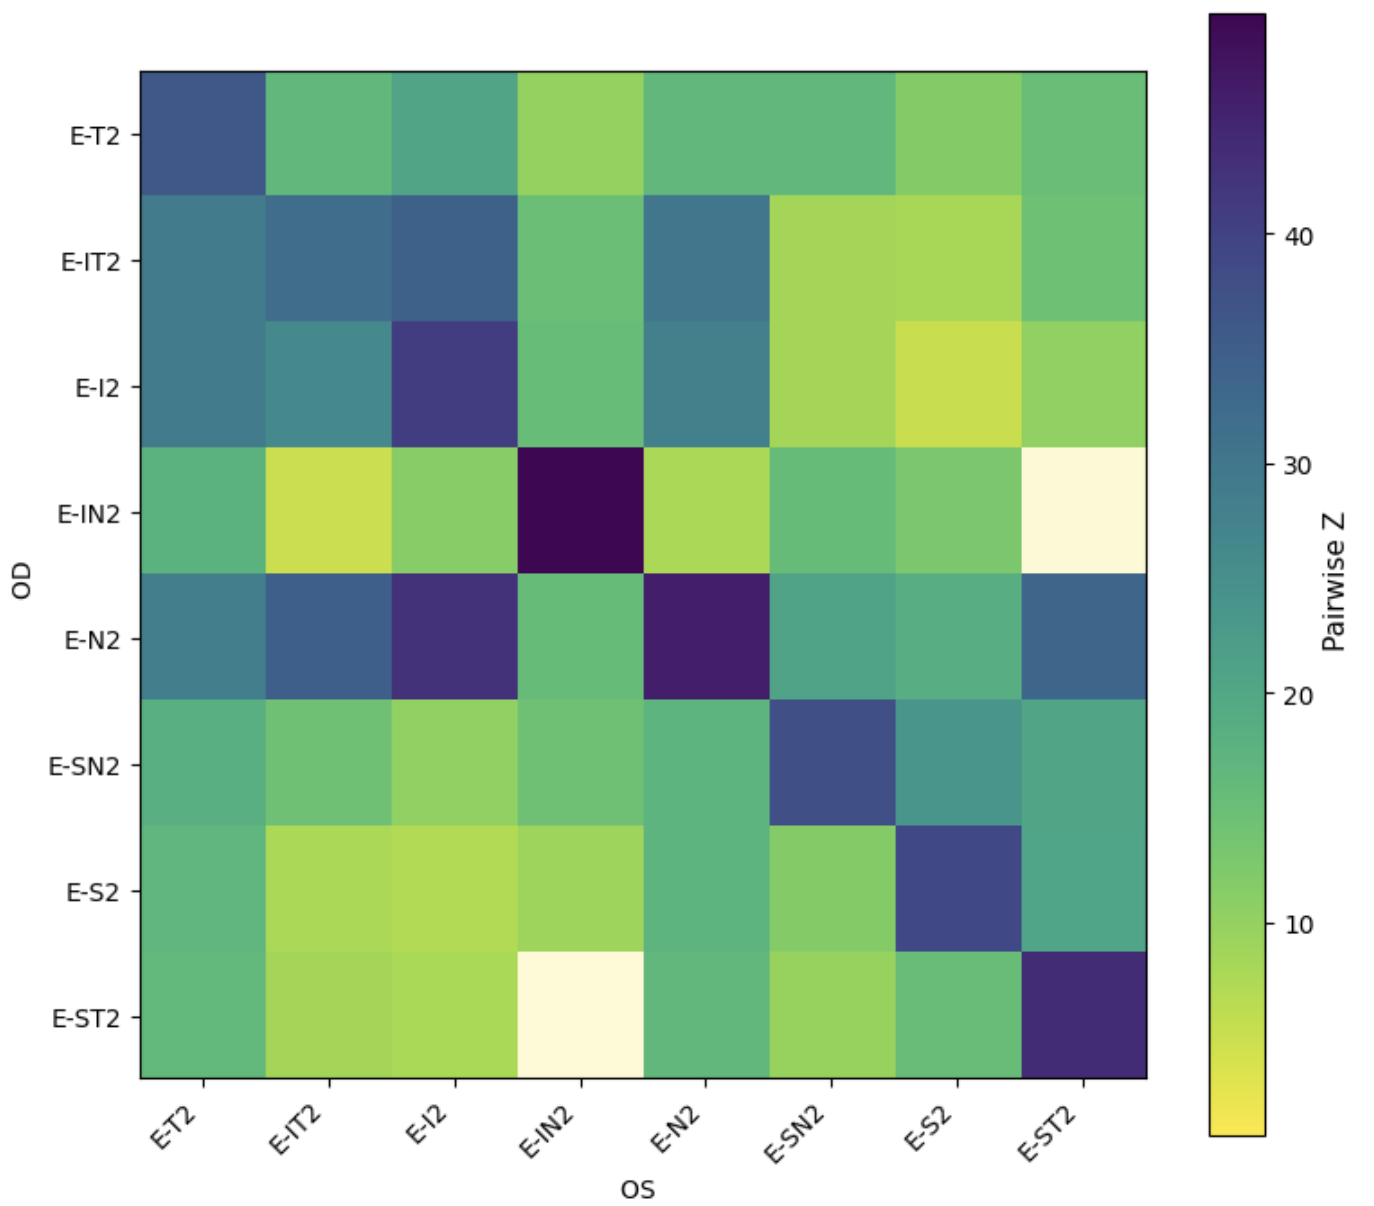
\includegraphics[
      trim=14pt 12pt 14pt 12pt,clip,
      width=0.34\columnwidth,height=0.2\textheight,keepaspectratio
    ]{plots/region_2.png}\hspace{-0.6em}%
    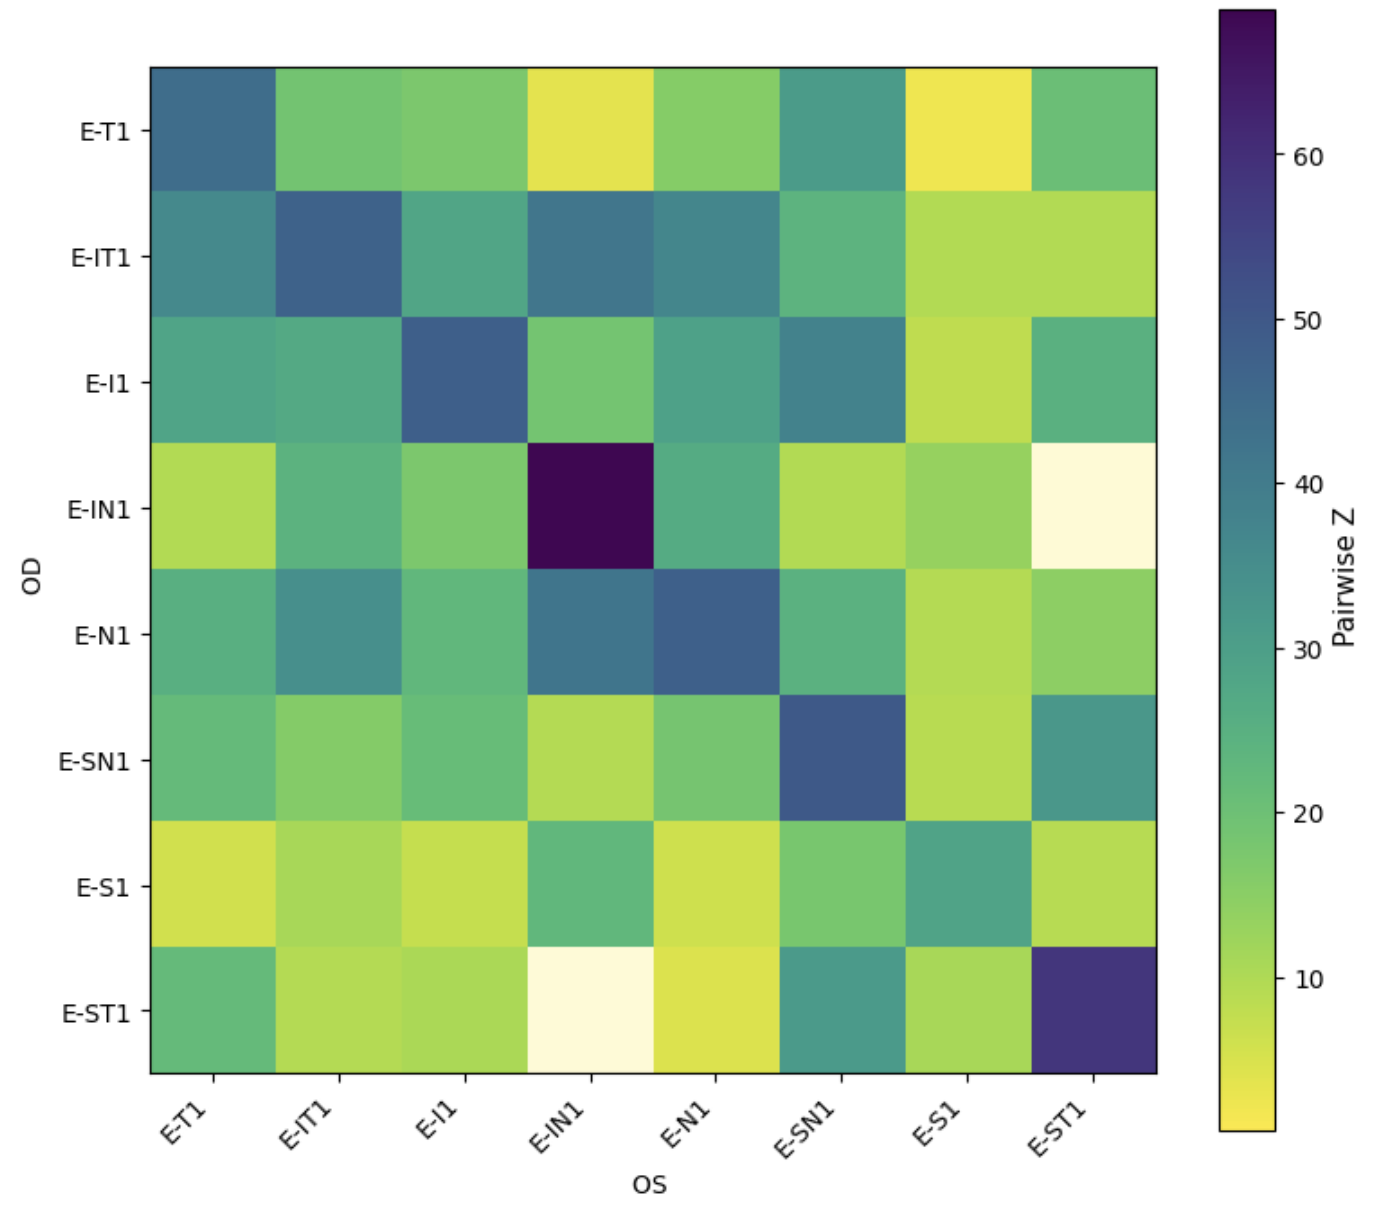
\includegraphics[
      trim=14pt 12pt 14pt 12pt,clip,
      width=0.34\columnwidth,height=0.2\textheight,keepaspectratio
    ]{plots/region_1.png}

    \caption{\scriptsize
    wa-dCoBET dependence heatmaps for corneal epithelial thickness regions, X-axis is the OD regions and Y-axis is the OS regions:
    left: Section~1 ($p=q=10$; central + inner ring); middle: Section~2 ($p=q=8$; middle ring);
    right: Section~3 ($p=q=8$; outer ring).
    Strong OD--OS correspondence is visible across all sections, with Section~1
    additionally exhibiting stronger within-eye coupling among central subregions.
    }
    \label{fig:eye_heatmaps_3sections}
    \vspace{-0.6em}
\end{figure}

\section{Conclusion}
\label{sec:conclusion}

We introduced a binary-expansion–based independence measure and established a general equivalence between testing independence and testing cross-covariances of binary expansion interaction coefficients for multivariate random variables. Unlike kernel-based measures such as HSIC, this equivalence holds over general spaces and does not rely on reproducing kernel Hilbert space assumptions. To address the computational challenges posed by the exponential growth of binary expansion coefficients, we developed an unbiased U-statistic and derived a scalable kernel representation that enables efficient computation. The proposed method admits a tractable asymptotic theory, eliminates the need for kernel selection, and flexibly truncates higher-order interactions to suppress noise, yielding robust power and improved interpretability.

We developed three complementary procedures: CoBET, a covariance-based test;
dCoBET, a weighted extension that incorporates multiscale structure in the
spirit of distance-based methods; and wa-dCoBET, an adaptive aggregation
procedure that combines multiple weighting schemes via foldwise
signal-to-noise-ratio voting. The resulting tests are tuning-free,
computationally efficient, and admit asymptotically exact Gaussian calibration
without permutation. Simulation studies demonstrate that wa-dCoBET delivers
substantial power gains in nonlinear and higher-dimensional settings, while the
real-data analysis of corneal epithelial thickness illustrates its
interpretability and practical relevance.

% \section{Copula-Based Data-Generating Mechanism and Simulation Results}
% \label{app:copula-dgm}
% \subsection{Data-Generating Mechanism}
% This section describes the copula-based data-generating mechanism used in the
% simulation studies.

% We generate covariates $\tilde{U} \in (0,1)^d$ with controlled internal dependence using
% a $d$-dimensional Clayton copula with parameter $\theta \ge 0$. Independently,
% we generate $\tilde{V} \sim \mathrm{Unif}(0,1)^d$, which enters $Y$ in the transformation
% functions considered in the simulation study.

% Dependence between the covariates and responses is controlled by a scalar
% parameter $b$. When $b=0$, the response depends only on $V$, yielding
% independence between $X$ and $Y$. When $b>0$, both $X$ and $Y$ depends on both $U$, inducing dependence between $X$ and $Y$.

% \subsection{Clayton Copula Construction}

% We generate dependent uniforms using the Gamma--Exponential representation of
% the Clayton copula. For each observation $i = 1,\ldots,n$ and $\theta > 0$, we
% draw
% \[
% S_i \sim \mathrm{Gamma}\!\left(\frac{1}{\theta}, 1\right),
% \qquad
% E_i^{(r)} \sim \mathrm{Exp}(1),
% \quad r = 1,\ldots,d,
% \]
% independently, and define
% \[
% \tilde{U}_i^{(r)}
% =
% \bigl(1 + E_i^{(r)} / S_i\bigr)^{-1/\theta},
% \qquad r = 1,\ldots,d.
% \]

% The resulting vector $\tilde{U}_i = (\tilde{U}_i^{(1)},\ldots,\tilde{U}_i^{(d)})$ follows a
% $d$-dimensional Clayton copula with parameter $\theta$ and uniform marginals.

% When $\theta = 0$, the coordinates of $\tilde{U}_i$ are generated independently from
% $\mathrm{Unif}(0,1)$, corresponding to the independence copula.

%\subsection{Noise Generation}
% Independently of $\{U_i\}_{i=1}^n$, we generate
% \[
% V_i \sim \mathrm{Unif}(0,1)^d,
% \qquad i = 1,\ldots,n,
% \]


% \subsection{Simulation results}

% Figures~\ref{fig:power-n250} and~\ref{fig:power-n1000} present additional
% empirical power curves for smaller ($n=250$) and larger ($n=1000$) sample sizes,
% respectively. These results complement the main analysis in
% Figure~\ref{fig:power-n500} and illustrate the stability of method comparisons
% across different sample regimes.

% For $n=250$, overall power is reduced across all procedures, particularly at
% small signal strengths, as expected. Nevertheless, the relative ordering of
% methods remains consistent with the main findings: wa-dCoBET continues to
% outperform competing tests under the LogQuad transformation and shows earlier
% detection in higher dimensions. Kernel-based methods exhibit more pronounced
% power degradation in complex and higher-dimensional settings.

% For $n=1000$, power increases uniformly across all alternatives, and most methods
% approach unit power at moderate values of $b$. Despite this, wa-dCoBET retains a
% clear advantage in terms of signal efficiency, achieving high power at smaller
% $b$ than competing approaches, especially under nonlinear and high-dimensional
% dependence. These patterns confirm that the improvements observed at $n=500$ are
% not artifacts of a particular sample size but persist across a broad range of
% $ n $.
% \begin{figure}[htbp]
%     \centering

%     \begin{subfigure}[t]{0.48\textwidth}
%         \centering
%         \includegraphics[width=\linewidth]{plots/dcobet_power_lines_n250.png}
%         \caption{$\dim(U)=\dim(V)=2$.}
%     \end{subfigure}
%     \hfill
%     \begin{subfigure}[t]{0.48\textwidth}
%         \centering
%         \includegraphics[width=\linewidth]{plots/dcobet_power_lines_dim10_n250.png}
%         \caption{$\dim(U)=\dim(V)=10$.}
%     \end{subfigure}

%     \caption{Empirical power comparison for sample size $n=250$.
%     Results correspond to the same dependence structures and testing
%     procedures as in Figure~\ref{fig:power-n500}.}
%     \label{fig:power-n250}
% \end{figure}
% \begin{figure}[htbp]
%     \centering

%     \begin{subfigure}[t]{0.48\textwidth}
%         \centering
%         \includegraphics[width=\linewidth]{plots/dcobet_power_lines_n1000.png}
%         \caption{$\dim(U)=\dim(V)=2$.}
%     \end{subfigure}
%     \hfill
%     \begin{subfigure}[t]{0.48\textwidth}
%         \centering
%         \includegraphics[width=\linewidth]{plots/dcobet_power_lines_dim10_n1000.png}
%         \caption{$\dim(U)=\dim(V)=10$.}
%     \end{subfigure}

%     \caption{Empirical power comparison for sample size $n=1000$.
%     Results correspond to the same dependence structures and testing
%     procedures as in Figure~\ref{fig:power-n500}.}
%     \label{fig:power-n1000}
% \end{figure}


\section{Detailed Proof of Theorems}
\label{theorem_proof}
\subsection{Proof of Theorem~\ref{thm:kernel-representation}}
\label{sec:proof-kernel-representation}

We prove the stated finite-depth expansion for
$\varphi_{UV}(t,s)-\varphi_U(t)\varphi_V(s)$.

\paragraph{Step 1: A single coordinate expansion.}
Fix a coordinate $r\in\{1,\dots,p\}$, a sample index $i$, and a truncation depth
$K\in\mathbb N$.
Using the truncated binary expansion
\[
U_i^{(r)}
= \sum_{k=1}^{\infty} 2^{-k} A^{(r)}_{k,i},
\qquad
A_{k,i}^{(r)}\in\{-1,+1\},
\]
we obtain
\[
e^{\jmath t_r U_i^{(r)}}
=
\prod_{k=1}^K e^{\jmath t_r 2^{-k}A_{k,i}^{(r)}}
=
\prod_{k=1}^K
\Bigl\{
\cos\!\bigl(t_r/2^k\bigr)
+ \jmath\,A_{k,i}^{(r)}\sin\!\bigl(t_r/2^k\bigr)
\Bigr\}.
\]
Expanding the product over $k$ yields a sum indexed by subsets
$I_r\subset\{1,\dots,K\}$:
\[
e^{\jmath t_r U_i^{(r)}}
=
\sum_{I_r\subset\{1,\dots,K\}}
\jmath^{|I_r|}
\Bigl(\prod_{k\in I_r} A_{k,i}^{(r)}\Bigr)
\Bigl(\prod_{k\in I_r}\sin(t_r/2^k)\Bigr)
\Bigl(\prod_{k\notin I_r}\cos(t_r/2^k)\Bigr).
\]
Define the one-dimensional basis functions
\[
\Pi_{I_r}(t_r)
:=
\Bigl(\prod_{k\in I_r}\sin(t_r/2^k)\Bigr)
\Bigl(\prod_{k\notin I_r}\cos(t_r/2^k)\Bigr),
\qquad I_r\subset\{1,\dots,K\},
\]
and the associated sample-level binary interaction
\[
\mathcal A_{i,I_r}^{(r)}
:=
\prod_{k\in I_r}A_{k,i}^{(r)},
\]
with the convention $\mathcal A_{i,\emptyset}^{(r)}=1$. Then
\[
e^{\jmath t_r U_i^{(r)}}
=
\sum_{I_r\subset\{1,\dots,K\}}
\jmath^{|I_r|}
\mathcal A_{i,I_r}^{(r)}\,
\Pi_{I_r}(t_r).
\]

\paragraph{Step 2: Multivariate factorization.}
Since
$e^{\jmath\langle t,U_i\rangle}=\prod_{r=1}^p e^{\jmath t_r U_i^{(r)}}$,
multiplying the coordinatewise expansions yields
\[
e^{\jmath\langle t,U_i\rangle}
=
\sum_{I\in\mathcal I_p^*}
\jmath^{|I|}
\mathcal A_{i,I}\,\Pi_I(t),
\qquad
|I|:=\sum_{r=1}^p |I_r|,
\]
where
\[
\mathcal A_{i,I}
:=
\prod_{r=1}^p \prod_{k\in I_r} A_{k,i}^{(r)},
\qquad
\Pi_I(t)
:=
\prod_{r=1}^p \Pi_{I_r}(t_r)
=
\prod_{r=1}^p
\Bigl(
\prod_{k\in I_r}\sin(t_r/2^k)
\prod_{k\notin I_r}\cos(t_r/2^k)
\Bigr).
\]
Analogously, for $V_i=(V_i^{(1)},\dots,V_i^{(q)})$ with binary coefficients
$B_{j,i}^{(s)}$, we have
\[
e^{\jmath\langle s,V_i\rangle}
=
\sum_{J\in\mathcal I_q}
\jmath^{|J|}
\mathcal B_{i,J}\,\Pi_J(s),
\qquad
\mathcal B_{i,J}
:=
\prod_{s=1}^q \prod_{j\in J_s} B_{j,i}^{(s)}.
\]

\paragraph{Step 3: Joint characteristic function expansion.}
Taking expectations over the i.i.d.\ sample $(U_i,V_i)$,
\[
\varphi_{UV}(t,s)
=
\mathbb E\!\left[
e^{\jmath\langle t,U_i\rangle}
e^{\jmath\langle s,V_i\rangle}
\right]
=
\sum_{I\in\mathcal I_p}
\sum_{J\in\mathcal I_q}
\jmath^{|I|+|J|}
\mathbb E(\mathcal A_{i,I}\mathcal B_{i,J})
\Pi_I(t)\Pi_J(s).
\]
Similarly,
\[
\varphi_U(t)\varphi_V(s)
=
\sum_{I\in\mathcal I_p^*}
\sum_{J\in\mathcal I_q^*}
\jmath^{|I|+|J|}
\mathbb E(\mathcal A_{i,I})\,
\mathbb E(\mathcal B_{i,J})
\Pi_I(t)\Pi_J(s).
\]
Subtracting yields
\[
\varphi_{UV}(t,s)-\varphi_U(t)\varphi_V(s)
=
\sum_{I\in\mathcal I_p^*}
\sum_{J\in\mathcal I_q^*}
\jmath^{|I|+|J|}
m_{I,J}\,
\Pi_I(t)\Pi_J(s),
\]
where
\[
m_{I,J}
:=
\mbox{Cov}\!\bigl(\mathcal A_{i,I},\mathcal B_{i,J}\bigr)
=
\mathbb E(\mathcal A_{i,I}\mathcal B_{i,J})
-
\mathbb E(\mathcal A_{i,I})\,
\mathbb E(\mathcal B_{i,J}).
\]
Finally, if $I=(\emptyset,\dots,\emptyset)$ or
$J=(\emptyset,\dots,\emptyset)$, then
$\mathcal A_{i,I}\equiv 1$ or $\mathcal B_{i,J}\equiv 1$, implying
$m_{I,J}=0$. Hence the sum was restricted to
$\mathcal I_p^\star$ and $\mathcal I_q^\star$, completing the proof.
\qed

\paragraph{Remarks for Theorem~\ref{thm:kernel-representation}.}
Theorem~\ref{thm:kernel-representation} expresses the deviation from independence
$\varphi_{UV}(t,s)-\varphi_U(t)\varphi_V(s)$ as a finite linear combination of
the binary--expansion covariance coefficients
\[
m_{I,J}=\mbox{Cov}(\mathcal A_{i,I},\mathcal B_{i,J}),
\]
with basis functions $\Pi_I(t)\Pi_J(s)$.
Any choice of non-negative weight matrices $(W_A,W_B)$ therefore induces a quadratic aggregation
of these coefficients through \eqref{eq:Xi-weighted-pop}.
Specific selections recover familiar tests within this framework:
CoBET corresponds to $W_A=I_{d_A}$ and $W_B=I_{d_B}$, while dCoBET corresponds to distance covariance-motivated weights that encode multiscale structure
across the binary--expansion indices.
\subsection{Unbiased $U$--statistic estimators}
\label{sec:Ustat-weighted}

Fix $K$ and let $A_i\in\mathbb R^{d_A}$ and $B_i\in\mathbb R^{d_B}$ denote the
binary--expansion feature vectors constructed from $(U_i,V_i)$, indexed by
$I\in\mathcal I_p^\star$ and $J\in\mathcal I_q^\star$, respectively.
Let $\mu_A:=\mathbb E(\vec A_i)$ and $\mu_B:=\mathbb E(\vec B_i)$, and define the centered
features $\tilde A_i:=\vec A_i-\mu_A$ and $\tilde B_i:=\vec B_i-\mu_B$.
Write
\[
\Sigma_{AB}:=\mbox{Cov}(\tilde A_i,\tilde B_i),
\qquad
\Sigma_{BA}=\Sigma_{AB}^\top.
\]
For non-negative definite weight matrices $W_A\succeq0$ and $W_B\succeq0$, recall the weighted population functional
\begin{equation}
\label{eq:Xi-weighted-pop}
\mathcal V_W^2(U,V):=\mbox{tr}\!\bigl(\Sigma_{AB}W_B\Sigma_{BA}W_A\bigr).   
\end{equation}

\paragraph{Population algebra.}
Using $\Sigma_{AB}=\mathbb E(\vec A \vec B^\top)-\mu_A\mu_B^\top$, we expand
\[
\begin{aligned}
V_W^2(U,V)
&= \mbox{tr}\!\Big(
\big(\mathbb E(\vec A \vec B^\top)-\mu_A\mu_B^\top\big)
W_B
\big(\mathbb E(\vec B \vec A^\top)-\mu_B\mu_A^\top\big)
W_A
\Big) \\
&= \mbox{tr}\!\big( \mathbb E(\vec A \vec B^\top)\,W_B\,\mathbb E(\vec B \vec A^\top)\,W_A \big)
- 2\,\mbox{tr}\!\big( \mathbb E(\vec A \vec B^\top)\,W_B\,\mu_B\mu_A^\top\,W_A \big) \\
&\qquad
+ \mbox{tr}\!\big( \mu_A\mu_B^\top\,W_B\,\mu_B\mu_A^\top\,W_A \big).
\end{aligned}
\]

\paragraph{Sample analogues.}
Let $\mathbb E_n$ denote the empirical mean. Motivated by the three population
trace terms above, define
\[
\begin{aligned}
T_{1n}^{(W)}
&:= \mbox{tr}\!\big( \mathbb E_n(\vec A\vec B^\top)\,W_B\,\mathbb E_n(\vec B\vec A^\top)\,W_A \big),\\
T_{2n}^{(W)}
&:= \mbox{tr}\!\big( \mathbb E_n(\vec A \vec B^\top)\,W_B\,\mathbb E_n(\vec B)\,\mathbb E_n(\vec A)^\top\,W_A \big),\\
T_{3n}^{(W)}
&:= \mbox{tr}\!\big( \mathbb E_n(\vec A)\,\mathbb E_n(\vec B)^\top\,W_B\,\mathbb E_n(\vec B)\,\mathbb E_n(\vec A)^\top\,W_A \big).
\end{aligned}
\]

Each term admits a symmetrized $U$--statistic representation:
\[
\begin{aligned}
T_{1n}^{(W)}
&=
\frac{1}{n(n-1)}
\sum_{i\neq j}
(\vec A_i^\top W_A \vec A_j)\,(\vec B_j^\top W_B \vec B_i),\\
T_{2n}^{(W)}
&=
\frac{1}{n(n-1)(n-2)}
\sum_{\substack{i\neq j\neq k }}
(\vec A_i^\top W_A \vec A_j)\,(\vec B_j^\top W_B \vec B_k),\\
T_{3n}^{(W)}
&=
\frac{1}{n(n-1)(n-2)(n-3)}
\sum_{\substack{i\neq j \neq k \neq \ell}}
(\vec A_i^\top W_A \vec A_j)\,(\vec B_k^\top W_B \vec B_\ell).
\end{aligned}
\]

Finally, define the weighted CoBET/dCoBET statistic
\[
T_n^{(W)}:=T_{1n}^{(W)}-2T_{2n}^{(W)}+T_{3n}^{(W)}.
\]

\paragraph{Unbiasedness.}
$T_n^{(W)}$ is an unbiased $U$--statistic estimator
of $V_W^2(U,V)$.

\subsection{Computational simplifications}
\label{computational_simp}
To reduce computational cost for $T_{2n}^{(W)}$ and $T_{3n}^{(W)}$, we exploit algebraic structure in the weighted
inner products appearing in $T_{2n}^{(W)}$ and $T_{3n}^{(W)}$.
Define the stacked feature vectors
\[
\vec C_i :=
\begin{pmatrix}
W_A^{1/2} \vec A_i\\
W_B^{1/2} \vec B_i
\end{pmatrix}
\in \mathbb{R}^{d_A+d_B},
\qquad i=1,\dots,n.
\]
Then
\[
\vec C_i^\top \vec C_j
=
\vec A_i^\top W_A \vec A_j
+
\vec B_i^\top W_B \vec B_j .
\]

Recall the weighted $U$--statistics
\[
\begin{aligned}
T_{1n}^{(W)}
&=
\frac{1}{n(n-1)}
\sum_{i\neq j}
(\vec A_i^\top W_A \vec A_j)(\vec B_j^\top W_B \vec B_i),\\
T_{2n}^{(W)}
&=
\frac{1}{n(n-1)(n-2)}
\sum_{i\neq j\neq k}
(\vec A_i^\top W_A \vec A_j)(\vec B_j^\top W_B \vec B_k),\\
T_{3n}^{(W)}
&=
\frac{1}{n(n-1)(n-2)(n-3)}
\sum_{i\neq j\neq k\neq \ell}
(\vec A_i^\top W_A \vec A_j)(\vec B_k^\top W_B \vec B_\ell).
\end{aligned}
\]

\paragraph{Simplification for $T_{2n}^{(W)}$.}
Observe that
\[
\vec C_i^\top \vec C_j\, \vec C_j^\top \vec C_k
=
\vec A_i^\top W_A \vec A_j\, \vec A_j^\top W_A \vec A_k
+
\,\vec A_i^\top W_A \vec A_j\, \vec B_j^\top W_B \vec B_k
+
\,\vec A_k^\top W_A \vec A_j\, \vec B_j^\top W_B \vec B_i
+
\vec B_i^\top W_B \vec B_j\, \vec B_j^\top W_B \vec B_k,
\]
which implies
\[
\sum_{i\neq j\neq k}\vec A_i^\top W_A \vec A_j\, \vec B_j^\top W_B \vec B_k
=
\frac{1}{2}
\sum_{i\neq j\neq k}\Big(
\vec C_i^\top \vec C_j\, \vec C_j^\top \vec C_k
-
\vec A_i^\top W_A \vec A_j\, \vec A_j^\top W_A \vec A_k
-
\vec B_i^\top W_B \vec B_j\, \vec B_j^\top W_B \vec B_k
\Big).
\]

Let $P_n^3 := n(n-1)(n-2)$. Substituting the above identity yields
\[
\begin{aligned}
P_n^3\, T_{2n}^{(W)}
=
\frac{1}{2}\Bigg[
&\sum_i \Big( \sum_{j\neq i} \vec C_i^\top \vec C_j \Big)^2
- \sum_{i\neq j} (\vec C_i^\top \vec C_j)^2 \\
&- \sum_i \Big( \sum_{j\neq i} \vec A_i^\top W_A \vec A_j \Big)^2
+ \sum_{i\neq j} (\vec A_i^\top W_A \vec A_j)^2 \\
&- \sum_i \Big( \sum_{j\neq i} \vec B_i^\top W_B \vec B_j \Big)^2
+ \sum_{i\neq j} (\vec B_i^\top W_B \vec B_j)^2
\Bigg].
\end{aligned}
\]

\paragraph{Simplification for $T_{3n}^{(W)}$.}
Similarly, using the same decomposition,
\[
\sum_{i\neq j\neq k\neq \ell} \vec A_i^\top W_A \vec A_j\, \vec B_k^\top W_B \vec B_\ell
=
\frac{1}{2}
\sum_{i\neq j\neq k\neq \ell}\Big(
\vec C_i^\top \vec C_j\, \vec C_k^\top \vec C_\ell
-
\vec A_i^\top W_A \vec A_j\, \vec A_k^\top W_A \vec A_\ell
-
\vec B_i^\top W_B \vec B_j\, \vec B_k^\top W_B \vec B_\ell
\Big).
\]
Let $P_n^4 := n(n-1)(n-2)(n-3)$. After combinatorial simplification,
\[
\begin{aligned}
P_n^4\, T_{3n}^{(W)}
=
\frac{1}{2}\Bigg\{
&\Big( \sum_{i\neq j} \vec C_i^\top \vec C_j \Big)^2
- 4\Bigg[
\sum_i \Big( \sum_{j\neq i} \vec C_i^\top \vec C_j \Big)^2
- \sum_{i\neq j} (\vec C_i^\top \vec C_j)^2
\Bigg] \\
&- \Big( \sum_{i\neq j} \vec A_i^\top W_A \vec A_j \Big)^2
+ 4\Bigg[
\sum_i \Big( \sum_{j\neq i} \vec A_i^\top W_A \vec A_j \Big)^2
- \sum_{i\neq j} (\vec A_i^\top W_A \vec A_j)^2
\Bigg] \\
&- \Big( \sum_{i\neq j} \vec B_i^\top W_B \vec B_j \Big)^2
+ 4\Bigg[
\sum_i \Big( \sum_{j\neq i} \vec B_i^\top W_B \vec B_j \Big)^2
- \sum_{i\neq j} (\vec B_i^\top W_B \vec B_j)^2
\Bigg]
\Bigg\}.
\end{aligned}
\]

\paragraph{Computational complexity.}
Both $T_{2n}^{(W)}$ and $T_{3n}^{(W)}$ can therefore be computed using only
pairwise inner products of $\{\vec C_i\}$, $\{\vec A_i\}$, and $\{\vec B_i\}$.
This reduces the computational complexity from $O(n^3)$ and $O(n^4)$ to
$O(n^2)$, making the proposed test scalable to large sample sizes.

\paragraph{Closed-form expression of $K^{(p)}$.}
Repeated application of product-to-sum identities yields the finite
sine--series expansion
\[
\Pi_I(t)
=
\sum_{\lambda\in\Lambda_I}
c_{I,\lambda}\,
\sin(\langle\lambda,t\rangle+\phi_{I,\lambda}),
\quad
\Lambda_I\subset\{\pm 2^{-1},\dots,\pm 2^{-K}\}^p,
\quad
\phi_{I,\lambda}\in\{0,\tfrac{\pi}{2}\}.
\]
Substituting this expansion into the definition of $W_A(I,I')$ and using
the identity
\[
\frac{1}{c_p}
\int_{\mathbb R^p}
\frac{1-\cos\langle t,x\rangle}{\|t\|^{p+1}}\,dt
=
\|x\|,
\]
we obtain the closed-form expression
\[
K^{(p)}_{I,I'}
=
\frac{1}{2}
\sum_{\lambda\in\Lambda_I}\sum_{\lambda'\in\Lambda_{I'}}
c_{I,\lambda}c_{I',\lambda'}
\cos(\phi_{I,\lambda}-\phi_{I',\lambda'})
\bigl(\|\lambda+\lambda'\|-\|\lambda-\lambda'\|\bigr).
\]
This representation makes $K^{(p)}$ explicit and computable for any fixed
$(p,K)$.

\subsection{Proof of Theorem~\ref{thm:computeATA}}
\label{proof_theorem2.2}
Recall that $\vec A_i=(\mathcal A_{i,I})_{I\in\mathcal I_p^\star}$ where
\[
\mathcal A_{i,I}
=
\prod_{r=1}^p\prod_{k\in I_r} A^{(r)}_{k,i},
\qquad I=(I_1,\dots,I_p)\in\mathcal I_p^\star.
\]

\paragraph{Step 1: factorization of $\vec A_i^\top \vec A_j$.}
By definition,
\[
\vec A_i^\top \vec A_j
=
\sum_{I\in\mathcal I_p^\star} \mathcal A_{i,I}\mathcal A_{j,I}
=
\sum_{I\in\mathcal I_p^\star}
\prod_{r=1}^p\prod_{k\in I_r}\bigl(A^{(r)}_{k,i}A^{(r)}_{k,j}\bigr).
\]
Let $x^{(r)}_k:=A^{(r)}_{k,i}A^{(r)}_{k,j}$.
Using the elementary identity
\[
\sum_{S\subseteq\{1,\dots,K\}} \prod_{k\in S} x_k
=
\prod_{k=1}^K (1+x_k),
\]
we obtain, for each coordinate $r$,
\[
\sum_{I_r\subseteq\{1,\dots,K\}}\prod_{k\in I_r} x^{(r)}_k
=
\prod_{k=1}^K \bigl(1+x^{(r)}_k\bigr).
\]
Multiplying over $r=1,\dots,p$ gives
\[
\sum_{I\in\mathcal I_p}\prod_{r=1}^p\prod_{k\in I_r} x^{(r)}_k
=
\prod_{r=1}^p\prod_{k=1}^K \bigl(1+A^{(r)}_{k,i}A^{(r)}_{k,j}\bigr).
\]
The term corresponding to $I=(\emptyset,\dots,\emptyset)$ equals $1$. 
%and
%$\mathcal I_p^\star=\mathcal I_p\setminus\{(\emptyset,\dots,\emptyset)\}$,
Therefore
\[
\vec A_i^\top \vec A_j
=
\prod_{r=1}^p\prod_{k=1}^K \bigl(1+A^{(r)}_{k,i}A^{(r)}_{k,j}\bigr)-1,
\]
which proves \eqref{eq:A-dot-factorization}.

\paragraph{Step 2: integral representation of $\vec A_i^\top W_A \vec A_j$.}
Assume $W_A$ is defined via the Gram construction
\[
W_A(I,I')
=
\frac{1}{c_p}
\int_{\mathbb R^p} \Pi_I(t)\,\Pi_{I'}(t)\,w_0^2(t)\,dt,
\qquad I,I'\in\mathcal I_p^\star,
\]
where $\Pi_I(t)$ is the basis function in
Theorem~\ref{thm:kernel-representation}.
Then
\[
\vec A_i^\top W_A \vec A_j
=
\sum_{I,I'\in\mathcal I_p^\star}\mathcal A_{i,I}\,W_A(I,I')\,\mathcal A_{j,I'}
=
\frac{1}{c_p}\int_{\mathbb R^p}
\Bigl(\sum_{I\in\mathcal I_p^\star}\mathcal A_{i,I}\Pi_I(t)\Bigr)
\Bigl(\sum_{I'\in\mathcal I_p^\star}\mathcal A_{j,I'}\Pi_{I'}(t)\Bigr)
w_0^2(t)\,dt.
\]

Next, use the coordinatewise factorization
\[
\Pi_I(t)
=
\prod_{r=1}^p
\left(
\prod_{k\in I_r}\sin\frac{t_r}{2^k}
\prod_{k\notin I_r}\cos\frac{t_r}{2^k}
\right)
=
C(t)\,
\prod_{r=1}^p\prod_{k\in I_r}\tan\!\Bigl(\frac{t_r}{2^k}\Bigr),
\]
where
\[
C(t):=\prod_{r=1}^p\prod_{k=1}^K \cos\!\left(\frac{t_r}{2^k}\right),
\qquad
\pi_k^{(r)}(t):=\tan\!\left(\frac{t_r}{2^k}\right).
\]
Thus
\[
\sum_{I\in\mathcal I_p^\star}\mathcal A_{i,I}\Pi_I(t)
=
C(t)\sum_{I\in\mathcal I_p^\star}
\prod_{r=1}^p\prod_{k\in I_r}\Bigl(A^{(r)}_{k,i}\,\pi_k^{(r)}(t)\Bigr).
\]
Applying the same subset-sum identity as in Step~1 (and subtracting the empty
multi-index term) gives
\[
\sum_{I\in\mathcal I_p^\star}\mathcal A_{i,I}\Pi_I(t)
=
C(t)\left\{
\prod_{r=1}^p\prod_{k=1}^K\bigl(1+A^{(r)}_{k,i}\,\pi_k^{(r)}(t)\bigr)-1
\right\}.
\] 
This completes the proof.\qed


\paragraph{Remarks for Theorem~\ref{thm:computeATA}.} In particular, 
if $w_0^2(t)=\prod _{r=1}^p w_{0r}^2(t_r)$, the formula for $\vec A_i^\top W_A \vec A_j$ can be written as the product with marginal integrations, 
\begin{align*}
\vec A_i^\top W_A \vec A_j
&=
\prod_{r=1}^p\prod_{k=1}^K
\int \bigl(1+A^{(r)}_{k,i}\pi_k^{(r)}(t_r)\bigr)\bigl(1+A^{(r)}_{k,j}\pi_k^{(r)}(t_r)\bigr)\cos^2(t_r/2^k)w_{0r}^2(t_r)dt_r\\
&-\prod_{r=1}^p\prod_{k=1}^K\int
\bigl(1+A^{(r)}_{k,i}\pi_k^{(r)}(t_r)\bigr)\cos^2(t_r/2^k)w_{0r}^2(t_r)dt_r\\
&-\prod_{r=1}^p\prod_{k=1}^K\int
\bigl(1+A^{(r)}_{k,j}\pi_k^{(r)}(t_r)\bigr)\cos^2(t_r/2^k)w_{0r}^2(t_r)dt_r\\
&+\prod_{r=1}^p\prod_{k=1}^K\int\cos^2(t_r/2^k)w_{0r}^2(t_r)dt_r.
\end{align*}


\subsection{Proof of Theorem ~\ref{lem:leadingordervar}}

Let
\[
\tilde A_i := \vec A_i-\mathbb E(\vec A_i),\qquad
\tilde B_i := \vec B_i-\mathbb E(\vec B_i),
\]
and define the covariance matrices
\[
\Sigma_A := \mbox{Cov}(\tilde A_i)=\mathbb E(\tilde A_i\tilde A_i^\top),\qquad
\Sigma_B := \mbox{Cov}(\tilde B_i)=\mathbb E(\tilde B_i\tilde B_i^\top).
\]
Under $H_0:U\perp V$, the sequences $\{\tilde A_i\}_{i\ge1}$ and
$\{\tilde B_i\}_{i\ge1}$ are independent, and $\mathbb E(\tilde A_i)=0$,
$\mathbb E(\tilde B_i)=0$.

\paragraph{Step 1: Centering cancellation.}
By the explicit substitution $A_i=\tilde A_i+\mu_A$ and $B_i=\tilde B_i+\mu_B$
(with $\mu_A=\mathbb E(A_i)$ and $\mu_B=\mathbb E(B_i)$), expanding each of
$T_{1n}^{(W)},T_{2n}^{(W)},T_{3n}^{(W)}$ produces $16$ terms.
A direct coefficient bookkeeping over the index patterns
$(i,j)$, $(i,j,k)$, and $(i,j,k,\ell)$ shows that in the linear combination
$T_n^{(W)}:=T_{1n}^{(W)}-2T_{2n}^{(W)}+T_{3n}^{(W)}$, every term involving at
least one $\mu_A$ or $\mu_B$ cancels. Hence
\[
T_n^{(W)}=\tilde T_{1n}^{(W)}-2\tilde T_{2n}^{(W)}+\tilde T_{3n}^{(W)},
\]
where
\[
\tilde T_{1n}^{(W)}
=
\frac{1}{n(n-1)}\sum_{i\neq j}
\bigl(\tilde A_i^\top W_A \tilde A_j\bigr)\,
\bigl(\tilde B_i^\top W_B \tilde B_j\bigr),
\]
and $\tilde T_{2n}^{(W)},\tilde T_{3n}^{(W)}$ are defined analogously by
replacing $A$ and $B$ with $\tilde A$ and $\tilde B$ in the corresponding
three- and four-index $U$--statistics. In the following Steps 2-4, we provide details for computing variances $\tilde T_{1n}^{(W)}$. The variances of $\tilde T_{2n}^{(W)}$ and $\tilde T_{3n}^{(W)}$ can be obtained similarly and hence the details are omitted.

\paragraph{Step 2: Variance expansion for $\tilde T_{1n}^{(W)}$.}
Define, for $i\neq j$,
\[
X_{ij}^{(W)}
:=
\bigl(\tilde A_i^\top W_A \tilde A_j\bigr)\,
\bigl(\tilde B_i^\top W_B \tilde B_j\bigr),
\qquad
\tilde T_{1n}^{(W)}=\frac{1}{n(n-1)}\sum_{i\neq j} X_{ij}^{(W)}.
\]
Then
\[
\Var(\tilde T_{1n}^{(W)})
=
\mathbb E\big((\tilde T_{1n}^{(W)})^2\big)
-
\mathbb E^2(\tilde T_{1n}^{(W)}).
\]
Expand the square:
\[
\mathbb E\big((\tilde T_{1n}^{(W)})^2\big)
=
\frac{1}{n^2(n-1)^2}
\sum_{i\neq j}\sum_{k\neq \ell}
\mathbb E\!\left[X_{ij}^{(W)}X_{k\ell}^{(W)}\right].
\]
We now classify the pairs $(i,j)$ and $(k,\ell)$ by overlap pattern.
There are three cases:

\smallskip
\noindent
\emph{(a) identical ordered pairs: $(i,j)=(k,\ell)$.}
There are $n(n-1)$ such terms, contributing
\[
\sum_{i\neq j}\mathbb E\!\left[(X_{ij}^{(W)})^2\right]
=
n(n-1)\,\mathbb E\!\left[(X_{12}^{(W)})^2\right].
\]

\smallskip
\noindent
\emph{(b) one-index overlap: exactly one of $\{i,j\}$ equals one of $\{k,\ell\}$.}
A representative term is $\mathbb E(X_{ij}^{(W)}X_{i\ell}^{(W)})$ with distinct
$i,j,\ell$. By symmetry, all one-overlap terms reduce to either
$\mathbb E(X_{12}^{(W)}X_{13}^{(W)})$ or $\mathbb E(X_{12}^{(W)}X_{32}^{(W)})$,
which are equal under i.i.d.\ relabeling. The number of such ordered quadruples
$(i,j,k,\ell)$ is $4n(n-1)(n-2)$, so the total contribution is
\[
4n(n-1)(n-2)\,\mathbb E\!\left[X_{12}^{(W)}X_{13}^{(W)}\right].
\]

\smallskip
\noindent
\emph{(c) disjoint pairs: $\{i,j\}\cap\{k,\ell\}=\emptyset$.}
There are $n(n-1)(n-2)(n-3)$ such terms, each equal to
$\mathbb E(X_{12}^{(W)}X_{34}^{(W)})$ by symmetry.

\smallskip
Putting the three cases together,
\[
\begin{aligned}
\mathbb E\!\big[(\tilde T_{1n}^{(W)})^2\big]
&=
\frac{1}{n^2(n-1)^2}\Big(
  n(n-1)\,\mathbb E[(X_{12}^{(W)})^2] \\
&\qquad
+\,4n(n-1)(n-2)\,\mathbb E[X_{12}^{(W)}X_{13}^{(W)}] \\
&\qquad
+\,n(n-1)(n-2)(n-3)\,\mathbb E[X_{12}^{(W)}X_{34}^{(W)}]
\Big).
\end{aligned}
\]

Also,
\[
\mathbb E(\tilde T_{1n}^{(W)})
=
\frac{1}{n(n-1)}\sum_{i\neq j}\mathbb E(X_{ij}^{(W)})
=
\mathbb E(X_{12}^{(W)}),
\]
hence
\[
\mathbb E^2(\tilde T_{1n}^{(W)})=\mathbb E^2(X_{12}^{(W)}).
\]
Therefore,
\begin{align*}
\Var(\tilde T_{1n}^{(W)})
&=
\frac{1}{n^2(n-1)^2}\Big(
n(n-1)\,\mathbb E[(X_{12}^{(W)})^2]
+
4n(n-1)(n-2)\,\mathbb E[X_{12}^{(W)}X_{13}^{(W)}]\\
&\qquad\qquad\qquad\qquad\qquad\qquad
+
n(n-1)(n-2)(n-3)\,\mathbb E[X_{12}^{(W)}X_{34}^{(W)}]
\Big)
-
\mathbb E^2(X_{12}^{(W)}).
\end{align*}

\paragraph{Step 3: Simplifications under $H_0$.}
Under $H_0$, $\vec A_1$ and $\vec B_1$ are independent copies and
$\mathbb E(\tilde A_i)=\mathbb E(\tilde B_i)=0$, so
\[
\mathbb E(X_{12}^{(W)})
=
\mathbb E(\tilde A_1^\top W_A \tilde A_2)\,
\mathbb E(\tilde B_1^\top W_B \tilde B_2)
=0.
\]
Moreover, when $\{1,2\}$ and $\{3,4\}$ are disjoint, $X_{12}^{(W)}$ is independent
of $X_{34}^{(W)}$, hence

\begin{align*}
\mathbb E\!\left[X_{12}^{(W)}X_{34}^{(W)}\right]
&=
\mathbb E(X_{12}^{(W)})\,\mathbb E(X_{34}^{(W)})
=0\\
E[X_{12}^{(W)}X_{13}^{(W)}]
&=E[\bigl(\tilde A_1^\top W_A \tilde A_2\bigr)\,
\bigl(\tilde B_2^\top W_B \tilde B_1  \bigr)
\bigl(\tilde A_1^\top W_A \tilde A_3\bigr)\,
\bigl(\tilde B_3^\top W_B \tilde B_1\bigr)]=0.
\end{align*}

Thus the disjoint-pairs term vanishes, and the last subtraction also vanishes.
We obtain the exact variance decomposition
\[
\Var(\tilde T_{1n}^{(W)})
=
\frac{1}{n(n-1)}\,\mathbb E[(X_{12}^{(W)})^2].
\]
\paragraph{Step 4: closed-form evaluation of $\mathbb E[(X_{12}^{(W)})^2]$.}
Under $H_0$, $\tilde A$ and $\tilde B$ are independent, so
\[
\mathbb E[(X_{12}^{(W)})^2]
=
\mathbb E\big[(\tilde A_1^\top W_A \tilde A_2)^2\big]\;
\mathbb E\big[(\tilde B_1^\top W_B \tilde B_2)^2\big].
\]
We compute the first factor in detail:
\[
(\tilde A_1^\top W_A \tilde A_2)^2
=
\tilde A_1^\top W_A \tilde A_2\;\tilde A_2^\top W_A \tilde A_1
=
\tilde A_1^\top W_A\,(\tilde A_2\tilde A_2^\top)\,W_A \tilde A_1.
\]
Taking expectation and conditioning on $\tilde A_1$ gives
\[
\mathbb E\big[(\tilde A_1^\top W_A \tilde A_2)^2\big]
=
\mathbb E\!\left[
\tilde A_1^\top W_A\,\mathbb E(\tilde A_2\tilde A_2^\top)\,W_A \tilde A_1
\right]
=
\mathbb E\!\left[\tilde A_1^\top W_A\Sigma_A W_A \tilde A_1\right].
\]
Using $\mathbb E(\tilde A_1\tilde A_1^\top)=\Sigma_A$ and cyclicity of trace,
\[
\mathbb E\!\left[\tilde A_1^\top W_A\Sigma_A W_A \tilde A_1\right]
=
\mbox{tr}\!\left(W_A\Sigma_A W_A\,\mathbb E(\tilde A_1\tilde A_1^\top)\right)
=
\mbox{tr}(W_A\Sigma_A W_A\Sigma_A)
=
\|W_A\Sigma_A\|_F^2.
\]
Analogously,
\[
\mathbb E\big[(\tilde B_1^\top W_B \tilde B_2)^2\big]
=
\mbox{tr}(W_B\Sigma_B W_B\Sigma_B)
=
\|W_B\Sigma_B\|_F^2.
\]
Therefore,
\[
\mathbb E[(X_{12}^{(W)})^2]
=
\|W_A\Sigma_A\|_F^2\,\|W_B\Sigma_B\|_F^2.
\]

\paragraph{Step 5: conclude the leading-order variance.}
Substituting the expression for $\mathbb E[(X_{12}^{(W)})^2]$ yields
\[
\Var(\tilde T_{1n}^{(W)})
=
\frac{2}{n(n-1)}\|W_A\Sigma_A\|_F^2\,\|W_B\Sigma_B\|_F^2.
\]
Similar to the above computations, under the null hypothesis $H_0$, it 
can be shown that
\begin{align*}
\Var(\tilde T_{2n}^{(W)})
&=
\frac{4}{n(n-1)(n-2)}\|W_A\Sigma_A\|_F^2\,\|W_B\Sigma_B\|_F^2.\\
\Var(\tilde T_{3n}^{(W)})
&=
\frac{4}{n(n-1)(n-2)(n-3)}\|W_A\Sigma_A\|_F^2\,\|W_B\Sigma_B\|_F^2.
\end{align*}

In summary, we have $\Var(T_n^{(W)})=\Var(\tilde T_{1n}^{(W)})\{1+o(1)\}$ 
and
\[
\Var(T_n^{(W)})
=
\Var(\tilde T_{1n}^{(W)})\{1+o(1)\}
=
\frac{2}{n(n-1)}\|W_A\Sigma_A\|_F^2\,\|W_B\Sigma_B\|_F^2\{1+o(1)\},
\]
which is \eqref{eq:var-leading-general}.


\paragraph{Remarks for Theorem~\ref{lem:leadingordervar}.}
To estimate the leading-order variance, note that
\[
\|W_A\Sigma_A\|_F^2=\mbox{tr}(W_A\Sigma_AW_A\Sigma_A).
\]
A ratio-consistent estimator can be constructed via $U$--statistics mirroring
the bias-correction structure of $T_n^{(W)}$:
\[
\begin{aligned}
\widehat{\|W_A\Sigma_A\|_{\mathrm F}^2}
={}& \frac{1}{n(n-1)}\sum_{i\ne j}
   (\vec A_i^\top W_A \vec A_j)^2  \\
&\;-\frac{2}{\binom{n}{3}}\sum_{i\ne j\ne k}
   (\vec A_i^\top W_A \vec A_j)
   (\vec A_j^\top W_A \vec A_k)  \\
&\;+\frac{1}{\binom{n}{4}}\sum_{i\ne j\ne k\ne\ell}
   (\vec A_i^\top W_A \vec A_j)
   (\vec A_k^\top W_A \vec A_\ell).
\end{aligned}
\]

An estimator of $\|W_B\Sigma_B\|_{\mathrm F}^2$ is defined analogously.
Both estimators depend only on pairwise inner products
$\vec A_i^\top W_A \vec A_j$ and $\vec B_i^\top W_B \vec B_j$, which can be
computed efficiently using Theorem~\ref{thm:computeATA} without explicitly
expanding $\vec A_i$ and $\vec B_i$. \qed


\subsection{Proof of Theorem~\ref{thm:weighted-clt}}
\label{Normalization proof}

This proof verifies that the leading term of our statistic falls into the
degenerate RKHS $U$--statistic framework of \citet{HeZhongCuiMandrekar2023} and
that their Condition (C3) holds under our trace assumptions. Consequently, the
asymptotic normality result in \citet{HeZhongCuiMandrekar2023} applies to our
standardized statistic $Z_n^{(W)}$.

\subsubsection{Kernel representation of the leading term}
Under $H_0:U\perp V$, let
\[
\tilde A_i := \vec A_i-\mathbb E(\vec A_i),\qquad
\tilde B_i := \vec B_i-\mathbb E(\vec B_i),
\qquad
Z_i := (\tilde A_i,\tilde B_i).
\]
Recall that each binary feature is a product of $\pm1$ bits, hence every entry
of $\vec A_i$ and $\vec B_i$ takes values in $\{-1,+1\}$. Therefore each entry
of $\tilde A_i$ and $\tilde B_i$ is uniformly bounded in $[-1,1]$, implying in
particular that $\tilde A_i,\tilde B_i$ have finite moments of all orders and
are sub-Gaussian (with constants independent of dimension).

For deterministic symmetric matrices $W_A,W_B$, define the symmetric order--2
kernel
\[
K(Z_i,Z_j)
:=
(\tilde A_i^\top W_A \tilde A_j)\,
(\tilde B_i^\top W_B \tilde B_j),
\qquad i\neq j,
\]
and the associated $U$--statistic
\[
\tilde T_{1n}^{(W)}=\frac{1}{n(n-1)}\sum_{i\neq j}K(Z_i,Z_j).
\]
This matches the setup of \citet{HeZhongCuiMandrekar2023} with input $Z$ and
kernel $K$.

\subsubsection{The induced second-order kernel $K_2$}
Following \citet{HeZhongCuiMandrekar2023}, define
\[
K_2(z,z') := \mathbb E\!\left\{ K(z,Z)\,K(Z,z')\right\}.
\]
Let
\[
\Sigma_A:=\mbox{Cov}(\tilde A),\qquad
\Sigma_B:=\mbox{Cov}(\tilde B).
\]
Under $H_0$, $\tilde A\perp \tilde B$, so for $z=(a,b)$ and $z'=(a',b')$,
\[
K_2\big((a,b),(a',b')\big)
=
(a^\top W_A\Sigma_AW_A a')\,(b^\top W_B\Sigma_BW_B b').
\]
Define also
\[
Q_A:=W_A\Sigma_AW_A,\qquad Q_B:=W_B\Sigma_BW_B,
\]
and
\[
M_A:=\Sigma_A^{1/2}W_A\Sigma_A^{1/2},\qquad
M_B:=\Sigma_B^{1/2}W_B\Sigma_B^{1/2}.
\]
Then
\[
\mbox{tr}(M_A^2)=\mbox{tr}(W_A\Sigma_AW_A\Sigma_A)=\|W_A\Sigma_A\|_F^2,
\qquad
\mbox{tr}(M_B^2)=\|W_B\Sigma_B\|_F^2.
\]

\subsubsection{Spectral factorization and the quantities $V_2,V_4$}
Let $\mathcal K$ be the integral operator $(\mathcal K f)(z)=\int K(z,z')f(z')
\,dP(z')$ under $H_0$. Because $P=P_{\tilde A}\otimes P_{\tilde B}$ and
\[
K\big((a,b),(a',b')\big)=K_A(a,a')\,K_B(b,b'),
\qquad
K_A(a,a'):=a^\top W_A a',\ \ K_B(b,b'):=b^\top W_B b',
\]
we have the tensor-product decomposition $\mathcal K=\mathcal K_A\otimes\mathcal K_B$.
Hence the eigenvalues of $\mathcal K$ are products of eigenvalues of
$\mathcal K_A$ and $\mathcal K_B$, and therefore
\[
V_2:=\sum_m\lambda_m^2
=
\Big(\sum_r\alpha_r^2\Big)\Big(\sum_s\beta_s^2\Big),
\qquad
V_4:=\sum_m\lambda_m^4
=
\Big(\sum_r\alpha_r^4\Big)\Big(\sum_s\beta_s^4\Big),
\]
where $\{\alpha_r\}$ and $\{\beta_s\}$ are eigenvalues of $\mathcal K_A$ and
$\mathcal K_B$, respectively. In our finite-dimensional linear-kernel setting,
these satisfy
\[
\sum_r\alpha_r^2=\mbox{tr}(M_A^2),\qquad \sum_r\alpha_r^4=\mbox{tr}(M_A^4),
\]
and similarly for $B$, so
\[
V_2=\mbox{tr}(M_A^2)\,\mbox{tr}(M_B^2),
\qquad
V_4=\mbox{tr}(M_A^4)\,\mbox{tr}(M_B^4).
\]

\subsubsection{Moment bounds for bilinear and quadratic forms}
We use the following standard bounds; the constants depend only on the
(sub-Gaussian) moment parameters of $\tilde A,\tilde B$, which are finite and
dimension-free because the coordinates are bounded (entries in $[-1,1]$).

\begin{lemma}[Bilinear/quadratic form moments]
\label{lem:bilinear-quad-moments}
Let $X,Y$ be independent, mean-zero, isotropic sub-Gaussian vectors in
$\mathbb R^d$ (i.e., $\mathbb E[XX^\top]=\mathbb E[YY^\top]=I_d$). Then for any
symmetric matrix $H$,
\[
\mathbb E[(X^\top H Y)^4]\;\le\; C_1\,\mbox{tr}(H^2)^2,
\qquad
\mathbb E[(X^\top H X)^2]\;\le\; C_2\{\mbox{tr}(H^2)+\mbox{tr}(H)^2\},
\]
where $C_1,C_2<\infty$ depend only on the sub-Gaussian norms of $X,Y$.
\end{lemma}

\subsubsection{Verification of Condition (C3) of \citet{HeZhongCuiMandrekar2023}}

\paragraph{Step 1: $\mathbb E\{K_2(Z_1,Z_2)^4\}=o(V_2^4)$.}
Under $H_0$,
\[
K_2(Z_1,Z_2)
=
(\tilde A_1^\top Q_A\tilde A_2)
(\tilde B_1^\top Q_B\tilde B_2),
\]
and independence implies
\[
\mathbb E\{K_2(Z_1,Z_2)^4\}
=
\mathbb E[(\tilde A_1^\top Q_A\tilde A_2)^4]\,
\mathbb E[(\tilde B_1^\top Q_B\tilde B_2)^4].
\]
Let $X_i=\Sigma_A^{-1/2}\tilde A_i$ and $Y_i=\Sigma_B^{-1/2}\tilde B_i$ so that
$\mathbb E[X_iX_i^\top]=I$ and $\mathbb E[Y_iY_i^\top]=I$. Then
\[
\tilde A_1^\top Q_A\tilde A_2
=
X_1^\top M_A^2 X_2,
\qquad
\tilde B_1^\top Q_B\tilde B_2
=
Y_1^\top M_B^2 Y_2.
\]
Applying Lemma~\ref{lem:bilinear-quad-moments} with $H=M_A^2$ and $H=M_B^2$,
\[
\mathbb E[(X_1^\top M_A^2 X_2)^4]\le C_1\,\mbox{tr}\!\big((M_A^2)^2\big)^2
= C_1\,\mbox{tr}(M_A^4)^2,
\]
and similarly
$\mathbb E[(Y_1^\top M_B^2 Y_2)^4]\le C_1\,\mbox{tr}(M_B^4)^2$.
Hence
\[
\mathbb E\{K_2(Z_1,Z_2)^4\}
\le
C_1^2\,\mbox{tr}(M_A^4)^2\,\mbox{tr}(M_B^4)^2.
\]
Since $V_2^4=\mbox{tr}(M_A^2)^4\,\mbox{tr}(M_B^2)^4$ and by assumption
\[
\mbox{tr}(M_A^4)=o(\mbox{tr}(M_A^2)^2),
\qquad
\mbox{tr}(M_B^4)=o(\mbox{tr}(M_B^2)^2),
\]
we conclude
\[
\mathbb E\{K_2(Z_1,Z_2)^4\}=o(V_2^4).
\]

\paragraph{Step 2: $\mathbb E\{K_2(Z_1,Z_1)^2\}=o(nV_2^2)$.}
We have
\[
K_2(Z_1,Z_1)
=
(\tilde A_1^\top Q_A\tilde A_1)
(\tilde B_1^\top Q_B\tilde B_1),
\]
so by independence
\[
\mathbb E\{K_2(Z_1,Z_1)^2\}
=
\mathbb E[(\tilde A_1^\top Q_A\tilde A_1)^2]\,
\mathbb E[(\tilde B_1^\top Q_B\tilde B_1)^2].
\]
Using $X_1=\Sigma_A^{-1/2}\tilde A_1$,
\[
\tilde A_1^\top Q_A\tilde A_1
=
X_1^\top M_A^2 X_1,
\]
and Lemma~\ref{lem:bilinear-quad-moments} yields
\[
\mathbb E[(X_1^\top M_A^2 X_1)^2]
\le
C_2\{\mbox{tr}((M_A^2)^2)+\mbox{tr}(M_A^2)^2\}
=
C_2\{\mbox{tr}(M_A^4)+\mbox{tr}(M_A^2)^2\}.
\]
Since $\mbox{tr}(M_A^4)=o(\mbox{tr}(M_A^2)^2)$, the RHS is
$O(\mbox{tr}^2(M_A^2))$; similarly,
$\mathbb E[(\tilde B_1^\top Q_B\tilde B_1)^2]=O(\mbox{tr}^2(M_B^2))$.
Therefore,
\[
\mathbb E\{K_2(Z_1,Z_1)^2\}
=
O\!\left(\mbox{tr}^2(M_A^2)\,\mbox{tr}^2(M_B^2)\right)
=
O(V_2^2),
\]
which implies
\[
\frac{\mathbb E\{K_2(Z_1,Z_1)^2\}}{nV_2^2}=O(1/n)\to 0,
\qquad\text{i.e.,}\qquad
\mathbb E\{K_2(Z_1,Z_1)^2\}=o(nV_2^2).
\]

\paragraph{Conclusion.}
Steps~1--2 verify Condition (C3) of \citet{HeZhongCuiMandrekar2023} for our
kernel. Combining this with our ratio-consistent variance estimator
$\widehat{\Var}(T_n^{(W)})$ and the degeneracy under $H_0$ yields
\[
Z_n^{(W)}=\frac{T_n^{(W)}}{\sqrt{\widehat{\mbox{Var}}(T_n^{(W)})}}
\;\stackrel{d}{\Rightarrow}\; \mathcal N(0,1),
\]
which establishes Theorem~\ref{thm:weighted-clt}. \qed


\subsection{Proof of Theorem~\ref{thm:alt-clt}}
\label{app:proof-alt-clt}

Under the alternative hypothesis $H_1: U\not\!\perp V$, define
\[
\tilde A_i=\vec A_i-\mathbb E(\vec A_i),
\qquad
\tilde B_i=\vec B_i-\mathbb E(\vec B_i),
\qquad
Z_i=(\tilde A_i,\tilde B_i).
\]
For deterministic symmetric weight matrices $W_A$ and $W_B$, define
\[
h(Z_i,Z_j)
=
(\tilde A_i^\top W_A\tilde A_j)
(\tilde B_i^\top W_B\tilde B_j),
\qquad i\ne j.
\]
Let
\[
T_n^{(W)}
=
\frac{1}{n(n-1)}
\sum_{i\ne j} h(Z_i,Z_j).
\]
Under $H_1$, the kernel is generally non-degenerate. Therefore, unlike the
null case, the first-order Hoeffding projection is the leading term.

Let
\[
\theta_W
=
\mathbb E\{h(Z_1,Z_2)\}.
\]
Since $Z_1$ and $Z_2$ are independent copies,
\[
\theta_W
=
\operatorname{tr}
\left(
W_A\Sigma_{AB}W_B\Sigma_{BA}
\right),
\]
where
\[
\Sigma_{AB}=\mathbb E(\tilde A\tilde B^\top),
\qquad
\Sigma_{BA}=\Sigma_{AB}^\top .
\]
Under $H_1$, $\Sigma_{AB}$ is generally nonzero, and hence $\theta_W$ may be
nonzero.

Define the first-order projection
\[
\psi(Z_i)
=
\mathbb E\{h(Z_i,Z_j)\mid Z_i\}-\theta_W .
\]
Because $Z_j$ is independent of $Z_i$,
\[
\mathbb E\{h(Z_i,Z_j)\mid Z_i\}
=
\tilde A_i^\top W_A\Sigma_{AB}W_B\tilde B_i .
\]
Thus,
\[
\psi(Z_i)
=
\tilde A_i^\top W_A\Sigma_{AB}W_B\tilde B_i-\theta_W .
\]
Let
\[
\sigma_{1,W}^2
=
\operatorname{Var}\{\psi(Z_1)\}
=
\operatorname{Var}
\left(
\tilde A^\top W_A\Sigma_{AB}W_B\tilde B
\right).
\]

By the Hoeffding decomposition,
\[
T_n^{(W)}-\theta_W
=
T_{1n}^{(W)}+T_{2n}^{(W)},
\]
where
\[
T_{1n}^{(W)}
=
\frac{2}{n}\sum_{i=1}^n \psi(Z_i)
\]
and
\[
T_{2n}^{(W)}
=
\frac{1}{n(n-1)}
\sum_{i\ne j} h_2(Z_i,Z_j),
\]
with
\[
h_2(Z_i,Z_j)
=
h(Z_i,Z_j)-\theta_W-\psi(Z_i)-\psi(Z_j).
\]
By construction,
\[
\mathbb E\{h_2(Z_i,Z_j)\mid Z_i\}=0,
\qquad
\mathbb E\{h_2(Z_i,Z_j)\mid Z_j\}=0.
\]
Therefore $T_{2n}^{(W)}$ is a degenerate second-order $U$-statistic.

If the full statistic contains additional terms from the expansion, write
\[
T_n-\theta_W
=
T_{1n}^{(W)}+T_{2n}^{(W)}+T_{3n}^{(W)},
\]
where $T_{3n}^{(W)}$ denotes the remaining higher-order degenerate component.
We will show that both $T_{2n}^{(W)}$ and $T_{3n}^{(W)}$ are negligible relative
to $T_{1n}^{(W)}$.

First,
\[
\operatorname{Var}(T_{1n}^{(W)})
=
\frac{4}{n}\sigma_{1,W}^2.
\]
This is the leading variance under $H_1$. Importantly, in the
high-dimensional setting, $\sigma_{1,W}^2$ may depend on $n$ through the
dimension. Therefore we compare all remainder terms to
$\operatorname{Var}(T_{1n}^{(W)})$ rather than bounding them by a fixed
low-dimensional rate.

Next, since $T_{2n}^{(W)}$ is a degenerate second-order $U$-statistic,
\[
\operatorname{Var}(T_{2n}^{(W)})
=
O\left\{
\frac{\mathbb E h_2^2(Z_1,Z_2)}{n^2}
\right\}.
\]
Using the boundedness of the binary expansion features and standard
quadratic-form moment bounds,
\[
\mathbb E h_2^2(Z_1,Z_2)
\le
C\,
\operatorname{tr}(W_A\Sigma_AW_A\Sigma_A)
\operatorname{tr}(W_B\Sigma_BW_B\Sigma_B),
\]
where
\[
\Sigma_A=\operatorname{Cov}(\tilde A),
\qquad
\Sigma_B=\operatorname{Cov}(\tilde B),
\]
and $C<\infty$ is a constant independent of $n$ and the dimension. Hence
\[
\operatorname{Var}(T_{2n}^{(W)})
=
O\left[
\frac{
\operatorname{tr}(W_A\Sigma_AW_A\Sigma_A)
\operatorname{tr}(W_B\Sigma_BW_B\Sigma_B)
}{n^2}
\right].
\]
Therefore,
\[
\frac{
\operatorname{Var}(T_{2n}^{(W)})
}{
\operatorname{Var}(T_{1n}^{(W)})
}
=
O\left[
\frac{
\operatorname{tr}(W_A\Sigma_AW_A\Sigma_A)
\operatorname{tr}(W_B\Sigma_BW_B\Sigma_B)
}{
n\sigma_{1,W}^2
}
\right].
\]
Assume that, under $H_1$,
\[
\frac{
\operatorname{tr}(W_A\Sigma_AW_A\Sigma_A)
\operatorname{tr}(W_B\Sigma_BW_B\Sigma_B)
}{
n\sigma_{1,W}^2
}
\to 0.
\tag{A1}
\]
Then
\[
\operatorname{Var}(T_{2n}^{(W)})
=
o\{\operatorname{Var}(T_{1n}^{(W)})\}.
\]

Similarly, for the higher-order degenerate component $T_{3n}^{(W)}$, standard
variance calculations for degenerate higher-order $U$-statistics give
\[
\operatorname{Var}(T_{3n}^{(W)})
=
O\left[
\frac{
\mathbb E h_3^2(Z_1,Z_2,Z_3)
}{n^3}
\right],
\]
where $h_3$ is the corresponding third-order degenerate projection. Again, by
boundedness of the binary expansion features and trace moment bounds,
\[
\mathbb E h_3^2(Z_1,Z_2,Z_3)
\le
C\,
\operatorname{tr}(W_A\Sigma_AW_A\Sigma_A)
\operatorname{tr}(W_B\Sigma_BW_B\Sigma_B).
\]
Thus,
\[
\operatorname{Var}(T_{3n}^{(W)})
=
O\left[
\frac{
\operatorname{tr}(W_A\Sigma_AW_A\Sigma_A)
\operatorname{tr}(W_B\Sigma_BW_B\Sigma_B)
}{n^3}
\right].
\]
Consequently,
\[
\frac{
\operatorname{Var}(T_{3n}^{(W)})
}{
\operatorname{Var}(T_{1n}^{(W)})
}
=
O\left[
\frac{
\operatorname{tr}(W_A\Sigma_AW_A\Sigma_A)
\operatorname{tr}(W_B\Sigma_BW_B\Sigma_B)
}{
n^2\sigma_{1,W}^2
}
\right].
\]
This is smaller than the corresponding ratio for $T_{2n}^{(W)}$. Therefore,
under condition (A1),
\[
\operatorname{Var}(T_{3n}^{(W)})
=
o\{\operatorname{Var}(T_{1n}^{(W)})\}.
\]
Hence,
\[
T_{2n}^{(W)}+T_{3n}^{(W)}
=
o_p\left(
\sqrt{\operatorname{Var}(T_{1n}^{(W)})}
\right).
\]

It remains to prove asymptotic normality of the leading term
$T_{1n}^{(W)}$. Define
\[
D_{n,i}
=
\frac{2}{n}\psi(Z_i),
\qquad
\mathcal F_i=\sigma(Z_1,\ldots,Z_i).
\]
Then
\[
T_{1n}^{(W)}
=
\sum_{i=1}^n D_{n,i}.
\]
Since $\mathbb E\{\psi(Z_i)\}=0$ and the observations are independent,
\[
\mathbb E(D_{n,i}\mid \mathcal F_{i-1})=0.
\]
Therefore $\{D_{n,i},\mathcal F_i\}_{i=1}^n$ is a martingale difference array.

We verify the martingale central limit theorem. First,
\[
\sum_{i=1}^n
\mathbb E(D_{n,i}^2\mid \mathcal F_{i-1})
=
\sum_{i=1}^n
\frac{4}{n^2}\mathbb E\{\psi^2(Z_i)\}
=
\frac{4\sigma_{1,W}^2}{n}
=
\operatorname{Var}(T_{1n}^{(W)}).
\]
Thus,
\[
\frac{
\sum_{i=1}^n
\mathbb E(D_{n,i}^2\mid \mathcal F_{i-1})
}{
\operatorname{Var}(T_{1n}^{(W)})
}
\stackrel{p}{\longrightarrow}1.
\]

Second, we verify the Lyapunov condition. We require
\[
\frac{
\sum_{i=1}^n \mathbb E(D_{n,i}^4)
}{
\operatorname{Var}^2(T_{1n}^{(W)})
}
\to 0.
\]
Since
\[
\sum_{i=1}^n \mathbb E(D_{n,i}^4)
=
n\cdot \frac{16}{n^4}\mathbb E\{\psi^4(Z_i)\}
=
\frac{16}{n^3}\mathbb E\{\psi^4(Z_i)\},
\]
and
\[
\operatorname{Var}^2(T_{1n}^{(W)})
=
\left(\frac{4\sigma_{1,W}^2}{n}\right)^2
=
\frac{16\sigma_{1,W}^4}{n^2},
\]
we have
\[
\frac{
\sum_{i=1}^n \mathbb E(D_{n,i}^4)
}{
\operatorname{Var}^2(T_{1n}^{(W)})
}
=
\frac{
\mathbb E\{\psi^4(Z_i)\}
}{
n\sigma_{1,W}^4
}.
\]
Assume
\[
\frac{
\mathbb E\{\psi^4(Z_i)\}
}{
n\sigma_{1,W}^4
}
\to 0.
\tag{A2}
\]
Then the Lyapunov condition holds. Therefore, by the martingale central limit
theorem,
\[
\frac{
T_{1n}^{(W)}
}{
\sqrt{\operatorname{Var}(T_{1n}^{(W)})}
}
\stackrel{d}{\longrightarrow}
N(0,1).
\]

Combining this with
\[
T_{2n}^{(W)}+T_{3n}^{(W)}
=
o_p\left(
\sqrt{\operatorname{Var}(T_{1n}^{(W)})}
\right),
\]
Slutsky's theorem yields
\[
\frac{
T_n^{(W)}-\theta_W
}{
\sqrt{\operatorname{Var}(T_{1n}^{(W)})}
}
\stackrel{d}{\longrightarrow}
N(0,1).
\]

Finally, since
\[
\operatorname{Var}(T_n^{(W)})
=
\operatorname{Var}(T_{1n}^{(W)})
\{1+o(1)\},
\]
we also have
\[
\frac{
T_n^{(W)}-\theta_W
}{
\sqrt{\operatorname{Var}(T_n^{(W)})}
}
\stackrel{d}{\longrightarrow}
N(0,1).
\]
If the variance estimator is ratio-consistent, namely
\[
\frac{
\widehat{\operatorname{Var}}(T_n^{(W)})
}{
\operatorname{Var}(T_n^{(W)})
}
\stackrel{p}{\longrightarrow}1,
\]
then another application of Slutsky's theorem gives
\[
\frac{
T_n^{(W)}-\theta_W
}{
\sqrt{\widehat{\operatorname{Var}}(T_n^{(W)})}
}
\stackrel{d}{\longrightarrow}
N(0,1).
\]
This proves the asymptotic normality of the proposed weighted statistic under
the alternative hypothesis. \qed
% \subsection{Proof of Theorem~\ref{thm:alt-clt}}
% \label{app:proof-alt-clt}

% Let
% \[
% \tilde A_i := \vec A_i-\mathbb E(\vec A_i),\qquad
% \tilde B_i := \vec B_i-\mathbb E(\vec B_i),\qquad
% Z_i:=(\tilde A_i,\tilde B_i),
% \]
% and define
% \[
% \Sigma_A := \mbox{Cov}(\tilde A_i)=\mathbb E(\tilde A_i\tilde A_i^\top),\qquad
% \Sigma_B := \mbox{Cov}(\tilde B_i)=\mathbb E(\tilde B_i\tilde B_i^\top).
% \]
% Throughout this proof we work under $H_1:U\not\!\perp V$.

% \paragraph{Step 1: Centering cancellation.}
% By the same bookkeeping argument as in Step~1 of the proof of
% Theorem~\ref{lem:leadingordervar}, in the linear combination
% $T_n^{(W)}:=T_{1n}^{(W)}-2T_{2n}^{(W)}+T_{3n}^{(W)}$, all terms involving
% $\mu_A:=\mathbb E(\vec A_i)$ or $\mu_B:=\mathbb E(\vec B_i)$ cancel. Hence
% \[
% T_n^{(W)}=\tilde T_{1n}^{(W)}-2\tilde T_{2n}^{(W)}+\tilde T_{3n}^{(W)},
% \]
% where
% \[
% \tilde T_{1n}^{(W)}
% =
% \frac{1}{n(n-1)}\sum_{i\neq j}
% (\tilde A_i^\top W_A \tilde A_j)\,
% (\tilde B_i^\top W_B \tilde B_j),
% \]
% and $\tilde T_{2n}^{(W)},\tilde T_{3n}^{(W)}$ are defined analogously by
% replacing $A,B$ with $\tilde A,\tilde B$.

% \paragraph{Step 2: Variance expansion for $\tilde T_{1n}^{(W)}$ (overlap patterns).}
% For $i\neq j$, define
% \[
% X_{ij}^{(W)}
% :=
% (\tilde A_i^\top W_A \tilde A_j)\,
% (\tilde B_i^\top W_B \tilde B_j),
% \qquad
% \tilde T_{1n}^{(W)}=\frac{1}{n(n-1)}\sum_{i\neq j}X_{ij}^{(W)}.
% \]
% Let
% \[
% \mu_W:=\mathbb E\!\left[X_{12}^{(W)}\right]
% =
% \mathbb E\!\left[
% (\tilde A_1^\top W_A \tilde A_2)(\tilde B_1^\top W_B \tilde B_2)
% \right]
% =
% \mathcal V_W^2(U,V).
% \]
% Expanding as in Step~2 of the proof of Theorem~\ref{lem:leadingordervar},
% \[
% \begin{aligned}
% \mathbb E\!\big[(\tilde T_{1n}^{(W)})^2\big]
% &=
% \frac{1}{n^2(n-1)^2}
% \Big[
%   n(n-1)\,\mathbb E\!\big[(X_{12}^{(W)})^2\big] \\
% &\qquad
% +4n(n-1)(n-2)\,\mathbb E\!\big[X_{12}^{(W)}X_{13}^{(W)}\big] \\
% &\qquad
% +n(n-1)(n-2)(n-3)\,\mathbb E\!\big[X_{12}^{(W)}X_{34}^{(W)}\big]
% \Big].
% \end{aligned}
% \]

% and
% \[
% \mathbb E(\tilde T_{1n}^{(W)})=\mu_W.
% \]
% Therefore,
% \begin{align}
% \label{eq:var-T1n-H1}
% \Var(\tilde T_{1n}^{(W)})
% &=
% \frac{1}{n(n-1)}\,
% \mathbb E\!\big[(X_{12}^{(W)})^2\big] \nonumber\\
% &\quad
% +\frac{4(n-2)}{n(n-1)}\,
% \mathbb E\!\big[X_{12}^{(W)}X_{13}^{(W)}\big] \nonumber\\
% &\quad
% +\frac{(n-2)(n-3)}{n(n-1)}\,
% \mathbb E\!\big[X_{12}^{(W)}X_{34}^{(W)}\big]
% -\mu_W^2 .
% \end{align}

% \paragraph{Step 3: Simplifications under $H_1$}
% When $\{1,2\}$ and $\{3,4\}$ are disjoint, $X_{12}^{(W)}$ and $X_{34}^{(W)}$
% are independent by i.i.d.\ sampling, hence
% \[
% \mathbb E[X_{12}^{(W)}X_{34}^{(W)}]
% =
% \mathbb E[X_{12}^{(W)}]\mathbb E[X_{34}^{(W)}]
% =
% \mu_W^2.
% \]
% Substituting into \eqref{eq:var-T1n-H1} yields
% \begin{align}
% \label{eq:var-T1n-H1-simplified}
% \Var(\tilde T_{1n}^{(W)})
% &=
% \frac{4(n-2)}{n(n-1)}
% \Big\{
%   \mathbb E\!\big[X_{12}^{(W)}X_{13}^{(W)}\big]
%   -\mu_W^2
% \Big\} \nonumber
% +\frac{1}{n(n-1)}
% \Big\{
%   \mathbb E\!\big[(X_{12}^{(W)})^2\big]
%   -\mu_W^2
% \Big\} \nonumber\\
% &\quad
% -\frac{4n-6}{n(n-1)}\,\mu_W^2
% +\frac{(n-2)(n-3)}{n(n-1)}\,\mu_W^2{\color{red}-\mu_W^2} \\[0.3em]
% &=
% \frac{4(n-2)}{n(n-1)}
% \Big\{
%   \mathbb E\!\big[X_{12}^{(W)}X_{13}^{(W)}\big]
%   -\mu_W^2
% \Big\} \nonumber +\frac{1}{n(n-1)}
% \Big\{
%   \mathbb E\!\big[(X_{12}^{(W)})^2\big]
%   -\mu_W^2
% \Big\}.
% \end{align}

% In particular,\footnote{We also need to compare orders between $E[X_{12}^{(W)}X_{13}^{(W)}]$ and $E\!\big[(X_{12}^{(W)})^2\big]$, in addition to the orders
% from $n$ and $n(n-1)$.}
% \begin{equation}
% \label{eq:var-T1n-leading}
% \Var(\tilde T_{1n}^{(W)})
% =
% \frac{4}{n}\Big(\mathbb E[X_{12}^{(W)}X_{13}^{(W)}]-\mu_W^2\Big)
% +O(n^{-2}).
% \end{equation}

% \paragraph{Step 4: Identify the leading constant via the first-order projection.}
% Define the first-order projection
% \[
% h_1(Z_1)
% :=
% \mathbb E\!\left[X_{12}^{(W)}\mid Z_1\right]-\mu_W.
% \]
% Then
% \[
% \Var\{h_1(Z_1)\}
% =
% \mathbb E\!\left[\Big(\mathbb E[X_{12}^{(W)}\mid Z_1]\Big)^2\right]-\mu_W^2.
% \]
% Using conditional independence of $Z_2$ and $Z_3$ given $Z_1$,
% \[
% \mathbb E[X_{12}^{(W)}X_{13}^{(W)}]
% =
% \mathbb E\!\left[
% \mathbb E[X_{12}^{(W)}\mid Z_1]\,
% \mathbb E[X_{13}^{(W)}\mid Z_1]
% \right]
% =
% \mathbb E\!\left[\Big(\mathbb E[X_{12}^{(W)}\mid Z_1]\Big)^2\right].
% \]
% Hence,
% \begin{equation}
% \label{eq:Cov-identity}
% \mathbb E[X_{12}^{(W)}X_{13}^{(W)}]-\mu_W^2
% =
% \Var\{h_1(Z_1)\}.
% \end{equation}
% This identification is the usual first-order Hoeffding-projection relation,
% and is also consistent with the orthogonal decomposition viewpoint used for
% $U$--statistics kernels in \citet{HeZhongCuiMandrekar2023}.

% Combining \eqref{eq:var-T1n-leading} and \eqref{eq:Cov-identity} gives
% \begin{equation}
% \label{eq:var-T1n-final}
% \Var(\tilde T_{1n}^{(W)})
% =
% \frac{4}{n}\Var\{h_1(Z_1)\}+O(n^{-2}).
% \end{equation}

% \paragraph{Step 5: The correction terms $\tilde T_{2n}^{(W)}$ and $\tilde T_{3n}^{(W)}$ are lower order under $H_1$.}
% The statistics $\tilde T_{2n}^{(W)}$ and $\tilde T_{3n}^{(W)}$ are (symmetric)
% $U$--statistics of orders $3$ and $4$ with bounded kernels (each entry of
% $\tilde A_i,\tilde B_i$ lies in $[-1,1]$ and $W_A,W_B$ are fixed). A standard
% overlap-pattern variance expansion analogous to Steps~2--3 shows\footnote{Similar to the previous notes, we need to check the variance of the third order and fourth order of U-statistics.}
% \[
% \Var(\tilde T_{2n}^{(W)})=O(n^{-2}),
% \qquad
% \Var(\tilde T_{3n}^{(W)})=O(n^{-3}),
% \]
% and similarly
% $\Cov(\tilde T_{1n}^{(W)},\tilde T_{2n}^{(W)})=O(n^{-2})$ and
% $\Cov(\tilde T_{1n}^{(W)},\tilde T_{3n}^{(W)})=O(n^{-2})$.
% Therefore,
% \[
% \Var\!\bigl(T_n^{(W)}\bigr)
% =
% \Var(\tilde T_{1n}^{(W)})\{1+o(1)\}
% =
% \frac{4}{n}\Var\{h_1(Z_1)\}\{1+o(1)\}.
% \]

% \paragraph{Step 6: Asymptotic normality.}
% By Step~1,
% \[
% \mathbb E\!\left[T_n^{(W)}\right]=\mu_W=\mathcal V_W^2(U,V).
% \]
% By the decomposition in Steps~2--5, the leading random fluctuation is driven by
% the one-overlap term, equivalently by the linear projection
% $h_1(Z_i)$, with variance of order $1/n$.
% Since $\{h_1(Z_i)\}_{i=1}^n$ are i.i.d.\ with $0<\Var(h_1)<\infty$, the classical
% CLT yields\footnote{Because the dimensions of the $A$ and $B$ are increasing with the sample size, the classical CLT would not work. Apply the CLT for triangular series. You may check the reference He et al. (2023). }
% \[
% \frac{2}{\sqrt n}\sum_{i=1}^n h_1(Z_i)
% \;\Rightarrow\;
% \mathcal N\!\left(0,\,4\,\Var\{h_1(Z_1)\}\right).
% \]
% Together with the fact that all remaining terms (including the contributions
% from $\tilde T_{2n}^{(W)}$ and $\tilde T_{3n}^{(W)}$) are $o_p(n^{-1/2})$, we obtain
% \[
% \sqrt n\Bigl(T_n^{(W)}-\mathcal V_W^2(U,V)\Bigr)
% \;\Rightarrow\;
% \mathcal N\!\left(0,\,4\,\Var\{h_1(Z_1)\}\right),
% \]
% which proves Theorem~\ref{thm:alt-clt}. \qed




\subsection{Worked Example: Binary--Expansion Feature Interactions}
\label{app:binary-example-new}

We illustrate the construction of the binary--expansion feature vector
$\vec A_i$ and enumerate all interaction terms in a simple low--dimensional
setting consistent with Section~\ref{binary_inde}.

\paragraph{Setup.}
Let $p=2$ and truncation depth $K=2$.
Let
\[
U_i = (U_i^{(1)}, U_i^{(2)}) \in [-1,1]^2
\]
denote the componentwise probability--integral transforms of
$(X^{(1)},X^{(2)})$.

For each coordinate $r\in\{1,2\}$, the truncated binary expansion is
\[
U_i^{(r)} = 2^{-1} A^{(r)}_{1,i} + 2^{-2} A^{(r)}_{2,i},
\qquad
A^{(r)}_{k,i} \in \{-1,+1\}.
\]

\paragraph{Binary coefficients.}
At depth $K=2$, each coordinate contributes two binary coefficients
\[
A^{(r)}_{1,i}, \quad A^{(r)}_{2,i},
\]
corresponding to the first and second dyadic resolution levels.

\paragraph{Index sets.}
For each coordinate $r$, the collection of nonempty subsets of
$\{1,2\}$ is
\[
\mathcal I^{(r)} = \bigl\{ \{1\}, \{2\}, \{1,2\} \bigr\}.
\]
The full multi--index set is
\[
\mathcal I_2^\star
=
\bigl\{
I=(I_1,I_2):
I_1,I_2 \in \mathcal I^{(r)} \cup \{\emptyset\},
\;
(I_1,I_2)\neq(\emptyset,\emptyset)
\bigr\}.
\]

\paragraph{Binary--expansion interactions.}
For $I=(I_1,I_2)\in\mathcal I_2^\star$, the interaction feature is
\[
\mathcal A_{i,I}
=
\prod_{r=1}^2 \;
\prod_{k\in I_r} A^{(r)}_{k,i}.
\]

\paragraph{All interaction terms.}
In this example, $\vec A_i$ contains $2^{pK}-1=15$ interaction features,
which we list explicitly below.

For illustration, when $p=2$ and $K=2$, the feature vector $\mathbf A_i$ contains the following $2^{4}-1=15$ interaction terms:
\[
\begin{aligned}
\mathbf A_i
=
(&
A^{(1)}_{1,i},
A^{(1)}_{2,i},
A^{(1)}_{1,i}A^{(1)}_{2,i},
A^{(2)}_{1,i},
A^{(2)}_{2,i},
A^{(2)}_{1,i}A^{(2)}_{2,i},\\
&
A^{(1)}_{1,i}A^{(2)}_{1,i},
A^{(1)}_{1,i}A^{(2)}_{2,i},
A^{(1)}_{2,i}A^{(2)}_{1,i},
A^{(1)}_{2,i}A^{(2)}_{2,i},\\
&
A^{(1)}_{1,i}A^{(1)}_{2,i}A^{(2)}_{1,i},
A^{(1)}_{1,i}A^{(1)}_{2,i}A^{(2)}_{2,i},
A^{(1)}_{1,i}A^{(2)}_{1,i}A^{(2)}_{2,i},\\
&
A^{(1)}_{2,i}A^{(2)}_{1,i}A^{(2)}_{2,i},
A^{(1)}_{1,i}A^{(1)}_{2,i}A^{(2)}_{1,i}A^{(2)}_{2,i}
).
\end{aligned}
\]

\paragraph{Feature vector.}
Stacking all interactions yields the binary--expansion feature vector
\[
\vec A_i
=
\bigl(
\mathcal A_{i,I}
\bigr)_{I\in\mathcal I_2^\star}
\;\in\;
\mathbb R^{15}.
\]

\paragraph{Interpretation.}
Each component of $\vec A_i$ corresponds to a multiscale interaction between
binary digits of $U_i^{(1)}$ and $U_i^{(2)}$. Theorem~\ref{thm:kernel-representation}
shows that dependence between $U$ and $V$ is fully characterized by the
cross--covariances between these interaction features and their analogues for
$V$.

\chapter{Testing Conditional Independence with Deep Neural Network Based Binary Expansion Testing (DeepBET)}
\label{DeepBET}
\noindent\textbf{Previously published as:}

Yang, Yang, Kai Zhang, and Ping-Shou Zhong. "Testing Conditional Independence with Deep Neural Network Based Binary Expansion Testing (DeepBET)." Proceedings of the 28th International Conference on Artificial Intelligence and Statistics (AISTATS 2025), Proceedings of Machine Learning Research, Vol. 258, pp. 4690–4698.


\section{Background Introduction}

Conditional independence (CI) plays a central role in modern statistics, machine learning, and artificial intelligence. Reliable CI testing is essential in many applications, including causal inference \cite{Pearl2009CausalII}, feature selection \cite{Cai2018FeatureSM}, and dimension reduction \cite{Waggoner_2021}. More broadly, CI testing provides a principled way to characterize relationships among variables, revealing whether associations persist after accounting for other factors. Consequently, CI testing has become an important tool in a wide range of domains, including information extraction, speech recognition, computer vision, genomics, and medical diagnosis.

\hspace{0.5cm}
This chapter focuses on testing whether two random variables, $X$ and $Y$, are conditionally independent after adjusting for a possibly high-dimensional set of covariates $Z$. Assuming the joint density of $(X,Y,Z)$ exists, conditional independence is defined by
\[
X \perp Y \mid Z
\]
whenever
\[
f(x,y\mid z)=f(x\mid z)f(y\mid z)
\]
for all $x$, $y$, and $z$ such that $f(z)>0$. Here,
$f(x,y\mid z)$ denotes the conditional joint density of $(X,Y)$ given $Z$, while
$f(x\mid z)$ and $f(y\mid z)$ are the corresponding conditional marginal densities (see, e.g., \cite{Shah_2020}). Accordingly, the conditional independence testing problem is formulated as
\[
H_0:X\perp Y\mid Z,
\qquad
H_1:X\not\!\perp Y\mid Z.
\]

The notation $\perp$ represents statistical independence, and ``$|$'' denotes conditioning. This chapter focuses on the challenging setting in which the conditioning variable $Z$ is high-dimensional, allowing its dimension $d$ to grow with the sample size $n$. In this regime, estimating the conditional distributions of $X$ and $Y$ given $Z$ becomes substantially more difficult because of the curse of dimensionality. The problem is particularly pronounced when the number of observations is relatively small compared with the dimension of the confounding variables.

\hspace{0.5cm}
A broad spectrum of methodologies has been developed for conditional independence testing, motivated by its fundamental role in statistical learning, causal inference, and machine learning applications. These methods differ considerably in both their modeling assumptions and computational strategies. One line of research constructs test statistics by comparing the conditional joint distribution of $(X,Y)$ given $Z$ with the product of the corresponding conditional marginal distributions. The effectiveness of these approaches relies heavily on the choice of discrepancy measure as well as the accuracy of the conditional distribution estimators. Another line of work estimates the conditional effects of $Z$ and subsequently examines the remaining association between $X$ and $Y$. Since conditional uncorrelatedness does not, in general, imply conditional independence, such methods may have limited sensitivity to nonlinear alternatives. Kernel-based techniques address this issue by embedding the variables into reproducing kernel Hilbert spaces, allowing a much richer class of nonlinear dependence structures to be detected, although their performance depends on the selected kernel. More recently, generative modeling approaches have been proposed to approximate conditional distributions by producing synthetic observations, offering considerable flexibility for analyzing high-dimensional and complex data.

\hspace{0.5cm}
As summarized in the survey of \cite{LiFan2020}, the existing literature can be broadly divided into four methodological families: regression-based methods (e.g., \cite{Shah_2020,Hoyer2008ANM,Zhang2017CausalDU,Zhang2023SCIT}), kernel-based methods (e.g., \cite{strobl2017approximate,Fukumizu2007KernelMO,zhang2012kernelbased}), distance-based methods (e.g., \cite{wang2015conditional,Su2014TestingCI,Su_White_2008,SuWhite2007}), and sampling-based methods (e.g., \cite{duong2022conditional,shi2021double,bellot2019conditional}).

\hspace{0.5cm}
Despite their successes, existing methods often exhibit one or more important shortcomings. Some procedures are not universally consistent and therefore have limited power against certain alternatives. Others struggle in high-dimensional settings because of the curse of dimensionality. Sampling-based approaches may also be computationally demanding and require careful tuning of multiple hyperparameters. As a consequence, many existing methods suffer from inflated type I error, reduced statistical power, substantial computational cost, or instability arising from parameter selection. Another common drawback is limited interpretability: many procedures simply report whether dependence exists without providing insight into its underlying structure. These limitations motivate the development of testing procedures that are simultaneously statistically reliable, computationally scalable, and interpretable. The proposed DeepBET framework is designed to address these challenges by combining deep neural networks (DNNs) with binary expansion testing (BET).

\hspace{0.5cm}
DeepBET integrates three complementary components: deep neural networks, binary expansion testing, and multiple sample splitting. To mitigate the curse of dimensionality, DNN models are first employed to estimate the conditional mean functions of $X$ and $Y$ given $Z$. Deep neural networks have demonstrated remarkable flexibility for modeling complex nonlinear relationships in high-dimensional data \cite{polson2018deep}. Recent theoretical work (e.g., \cite{Lu_2021,Bauer2019,schmidt2020nonparametric}) has established consistency and convergence properties for certain classes of DNN estimators under suitable optimization procedures \cite{Jentzen-JMLR-2022}. The residuals obtained from these fitted models are then analyzed using the binary expansion testing (BET) framework \cite{zhang2019bet}. BET enjoys desirable theoretical guarantees, including uniform consistency and minimax optimal sample complexity for detecting dependence \cite{zhang2019bet}, while also providing interpretable information about the form of dependence whenever the null hypothesis is rejected. Finally, a multiple-splitting strategy \cite{guo2024ranktransformed} is incorporated to further improve finite-sample power. The resulting procedure achieves effective type I error control while maintaining strong power across a broad range of alternatives.

\hspace{0.5cm}
Extensive simulation studies demonstrate that  \cite{pmlr-v258-yang25f} consistently achieves higher power than competing methods while maintaining accurate control of the type I error, particularly in challenging high-dimensional scenarios. In addition, its performance is relatively insensitive to the tuning parameters used for DNN estimation. Compared with existing sampling-based approaches (e.g., \cite{shi2021double,bellot2019conditional}), DeepBET is also computationally more efficient. Beyond testing for conditional independence, the proposed framework provides interpretable information regarding the structure of the detected dependence, which can facilitate subsequent statistical modeling and scientific investigation.

\hspace{0.5cm}
The remainder of this chapter is organized as follows. Section \ref{deepbet_proc} introduces the DeepBET methodology and establishes the asymptotic properties of the proposed test statistics. Section \ref{Numerical studies} reports simulation results together with an application to corneal epithelial thickness data from a dry eye disease study. Concluding remarks are given in Section \ref{discussion}, while all technical proofs are collected in Section \ref{tech_proof}.




\section{A DeepBET Procedure}
\label{deepbet_proc}

Let
\[
\{(X_i,Y_i,Z_i)\}_{i=1}^{n}
\]
be a sequence of independent and identically distributed observations, where the index set is
\[
\mathcal{S}=\{1,\ldots,n\}.
\]
We assume that the data are generated according to the additive noise models (ANMs)
\[
X_i=h(Z_i)+\epsilon_i,
\qquad
Y_i=g(Z_i)+\nu_i,
\]
where $h(\cdot)$ and $g(\cdot)$ are unknown regression functions that characterize the dependence of $X_i$ and $Y_i$ on the potentially high-dimensional confounding variables $Z_i$. Throughout this chapter, both $X_i$ and $Y_i$ are assumed to be univariate random variables, while the random errors $\epsilon_i$ and $\nu_i$ are independent of $Z_i$. The ANM assumption is introduced primarily to facilitate the theoretical derivation of the asymptotic null distribution of the proposed DeepBET statistics. As demonstrated in Section 3.2, the empirical performance of DeepBET remains competitive even when the data-generating mechanism does not satisfy the ANM assumption.

\hspace{0.5cm}
The proposed procedure begins by randomly partitioning the index set $\mathcal{S}$ into two disjoint subsets, denoted by $\mathcal{D}_1$ and $\mathcal{D}_2$, such that
\[
\mathcal{D}_1\cup\mathcal{D}_2=\mathcal{S},
\qquad
\mathcal{D}_1\cap\mathcal{D}_2=\emptyset.
\]
The first subset is used to estimate the conditional mean functions via deep neural networks (DNNs) \cite{LEE2021217}, whereas the second subset is reserved for constructing the conditional independence test statistic.

\hspace{0.5cm}
More specifically, DNN models are fitted using the observations in $\mathcal{D}_1$ to estimate the conditional expectations
\[
h(Z_j)=E(X_j\mid Z_j),
\qquad
g(Z_j)=E(Y_j\mid Z_j),
\qquad
j\in\mathcal{D}_1.
\]
Deep neural networks consist of multiple hidden layers that repeatedly transform the input through weighted linear combinations followed by nonlinear activation functions. This hierarchical architecture enables DNNs to approximate highly complex nonlinear regression functions in high-dimensional settings. The network architecture adopted in DeepBET is described in Section 3. Let
\[
\hat h_{\mathcal D_1}(Z_j)=\widehat E(X_j\mid Z_j),
\qquad
\hat g_{\mathcal D_1}(Z_j)=\widehat E(Y_j\mid Z_j),
\]
denote the fitted conditional mean estimators. These trained models are then applied to the observations in $\mathcal{D}_2$ to obtain predictions of the conditional means for $X_i$ and $Y_i$.

\hspace{0.5cm}
Using these fitted values, we compute the residuals
\[
\hat\epsilon_i=X_i-\hat h_{\mathcal D_1}(Z_i),
\qquad
\hat\nu_i=Y_i-\hat g_{\mathcal D_1}(Z_i),
\qquad
i\in\mathcal D_2,
\]
which serve as estimates of the unobservable noise variables $\epsilon_i$ and $\nu_i$. Conditional independence between $X$ and $Y$ given $Z$ is subsequently assessed by applying the Binary Expansion Testing (BET) procedure to the residual pairs $(\hat\epsilon_i,\hat\nu_i)$. Figure \ref{fig:DeepBET} illustrates the overall workflow of the proposed DeepBET framework.

\begin{figure}[ht!]
    \centering
    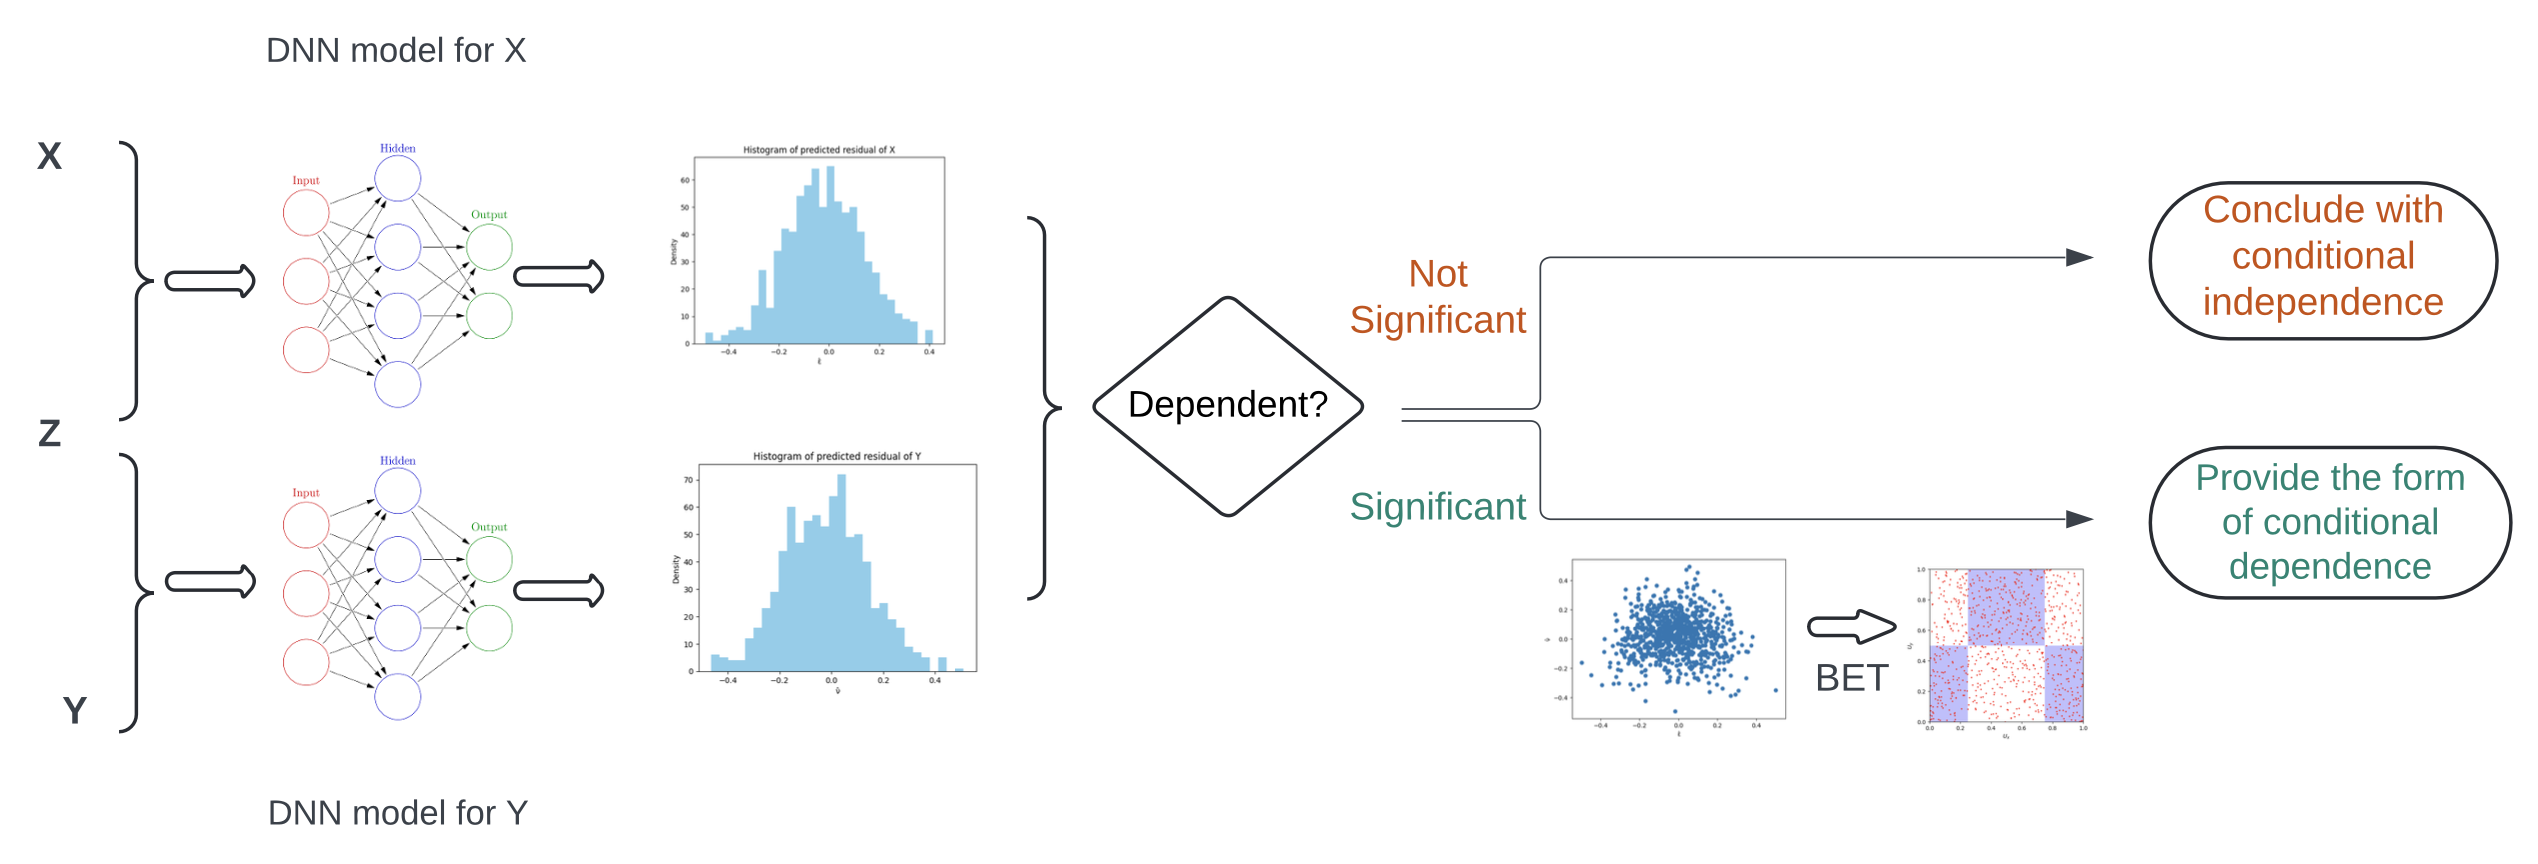
\includegraphics[
        width=0.9\textwidth,
        alt={DeepBET workflow showing sample splitting, neural-network
        estimation of conditional means, residual calculation, rank
        transformation, binary expansion, and independence testing
        of the transformed residuals.}
    ]{plots/DeepBET.png}
    \caption{Overview of the proposed DeepBET procedure. A deep neural network is first trained on one subset of the data to estimate the conditional mean functions of $X$ and $Y$ given $Z$. The fitted models are then used to obtain residuals from the remaining observations. Finally, Binary Expansion Testing (BET) is applied to the residuals to assess conditional independence.}
    \label{fig:DeepBET}
\end{figure}

\subsection{Binary Expansion Statistics}

Binary Expansion Testing (BET), originally proposed by \cite{zhang2019bet}, was developed as a distribution-free method for testing the independence of two random variables. BET possesses several attractive theoretical and practical properties. It is uniformly consistent against all fixed alternatives, achieves the minimax optimal detection rate, and provides interpretable information about the underlying dependence structure whenever the null hypothesis is rejected. Nevertheless, the original BET methodology was designed for unconditional independence and cannot be directly applied to conditional independence problems.

This chapter extends the BET framework to conditional independence testing through the proposed DeepBET procedure. A key advantage of binary expansion is its computational simplicity, since binary representations are straightforward to construct for continuous random variables after suitable transformations. More importantly, binary expansion converts the testing problem into one involving binary variables, for which zero correlation is equivalent to independence. This property forms the theoretical foundation for the consistency of the proposed DeepBET procedure.



%\subsubsection{Binary Expansion Filtration}

%Many distribution-free test lack of uniformity, the binary expansion filtration approach avoid such power loss.  


\hspace{0.5cm}
We first describe how the marginal binary expansions are constructed. Suppose that
$\{(U_i,V_i)\}_{i=1}^{n}$ are observations from bivariate random vectors whose marginal distributions are uniform on $[0,1]$. When the original marginals are not uniform, one may transform them through their distribution functions so that
$\tilde{U}=F_\epsilon(\epsilon)$ and $\tilde{V}=G_\nu(\nu)$
follow the uniform distribution on $[0,1]$, where
$F_\epsilon(\cdot)$ and $G_\nu(\cdot)$ are the marginal cumulative distribution functions of $\epsilon$ and $\nu$, respectively. When these marginal distributions are unavailable, they may be replaced by their empirical cumulative distribution functions, resulting in transformed observations that lie on the discrete grid
$\{1/n,\ldots,1\}$. In the DeepBET procedure, we apply empirical CDF transformations to the residuals $\hat{\epsilon}$ and $\hat{\nu}$, since their marginal distributions are unknown.

\hspace{0.5cm}
The binary expansions of the transformed variables are written as
\begin{center}
  $\hat{U}_i= \sum_{k=1}^{\substack{\infty}}(\hat{A}_i^{(k)}+1)/{{2}^{k+1}},  \hat{V}_i = \sum_{k=1}^{\substack{\infty}}(\hat{B}_i^{(k)}+1)/{{2}^{k+1}}$
\end{center}
where $\hat{A}_i^{(k)}$ and $\hat{B}_i^{(k)}$ are Bernoulli-type coefficients taking values in $\{-1,+1\}$. For implementation, these infinite expansions are truncated at depths $d_1$ and $d_2$, respectively:
\begin{align*}
   \hat{U}_{i,d}\!&=\!\sum_{k=1}^{\substack{d_1}}(\hat{A}_i^{(k)}\!+\!1)/{{2}^{k+1}}\;\mbox{and}\; 
   \hat{V}_{i,d}\!=\!\sum_{k=1}^{\substack{d_2}}(\hat{B}_i^{(k)}\!+\!1)/{{2}^{k+1}}.
\end{align*}

For fixed $d_1$ and $d_2$, the truncated variables $\hat{U}_{d_1}$ and $\hat{V}_{d_2}$ are discrete multinomial variables with $2^{d_1}$ and $2^{d_2}$ possible values, respectively. As the truncation depths increase, $\hat{U}_{i,d_1}$ and $\hat{V}_{i,d_2}$ converge in probability to $\hat{U}_i$ and $\hat{V}_i$. Thus, the joint distribution of $(\hat{U},\hat{V})$ can be approximated by the joint distribution of $(\hat{U}_{d_1},\hat{V}_{d_2})$. We refer to statistics formed from the binary coefficients $\hat{A}_{k}$ and $\hat{B}_{k}$ as BET statistics, and we refer to the corresponding independence testing framework for $(\hat{U}_{d_1},\hat{V}_{d_2})$ as BET at depths $d_1$ and $d_2$.

\hspace{0.5cm}
The pair $(\hat{U}_{i,d_1},\hat{V}_{i,d_2})$ has at most $2^{d_1+d_2}$ possible outcomes. Equivalently, the truncation partitions the unit square $[0,1]\times[0,1]$ into a $2^{d_1}\times 2^{d_2}$ grid. Therefore, the binary expansion representation converts the conditional dependence problem into a finite-dimensional grid-based problem, analogous to a contingency table, whose cell probabilities are identifiable.

\hspace{0.5cm}
To define the BET statistic rigorously, consider the filtration generated by $\{\hat{A}^{(k)}\}_{k=1}^{d_1}$ and $\{\hat{B}^{(k)}\}_{k=1}^{d_2}$ for each pair of depths $d_1$ and $d_2$. This filtration is denoted by $\sigma(U_{d_1},V_{d_2})$ and is the $\sigma$-field generated by
$\{\hat{A}^{(1)},\ldots,\hat{A}^{(d_1)},\hat{B}^{(1)},\ldots,\hat{B}^{(d_2)}\}$.
Let $\mathbf{a}$ and $\mathbf{b}$ be binary indicator vectors of lengths $d_1$ and $d_2$, respectively. The pair $\mathbf{a}\mathbf{b}$ indexes an element of the $\sigma$-field $\sigma(\hat{U}_{d_1},\hat{V}_{d_2})$, where an entry equal to $1$ indicates that the corresponding binary coefficient is included in the interaction. For $i\in\mathcal{D}_2$, define
\[
\hat{\mathcal{A}}_i^{\mathbf{a}}
=
\prod_{k=1}^{d_1}
\{\hat{A}_{i}^{(k)}\}^{a_k},
\qquad
\hat{\mathcal{B}}_i^{\mathbf{b}}
=
\prod_{k=1}^{d_2}
\{\hat{B}_{i}^{(k)}\}^{b_k}.
\]
The corresponding symmetry statistic is
\begin{center}
$\hat{S}_{(\mathbf{ab}),n}=\sum_{i\in\mathcal{D}_2}\hat{\mathcal{A}}_i^{\mathbf{a}}\hat{\mathcal{B}}_i^{\mathbf{b}},$
\end{center}
which measures the imbalance between observations satisfying
$\hat{\mathcal{A}}_i^{\mathbf{a}}\hat{\mathcal{B}}_i^{\mathbf{b}}=1$
and those satisfying
$\hat{\mathcal{A}}_i^{\mathbf{a}}\hat{\mathcal{B}}_i^{\mathbf{b}}=-1$, for $\mathbf{a}\neq0$ and $\mathbf{b}\neq0$.

\hspace{0.5cm}
The following example illustrates how the BET representation can reveal dependence patterns that are difficult to identify visually from the residual scatter plot. The residuals are generated from the nonlinear model described in Section \ref{simulation_results}, where the conditional dependence between $X$ and $Y$ given $Z$ is not immediately apparent from the raw residual plot.

\begin{figure}[h]
    \centering

    % Left panel: residual plot
    \begin{minipage}{0.45\textwidth}
        \centering
        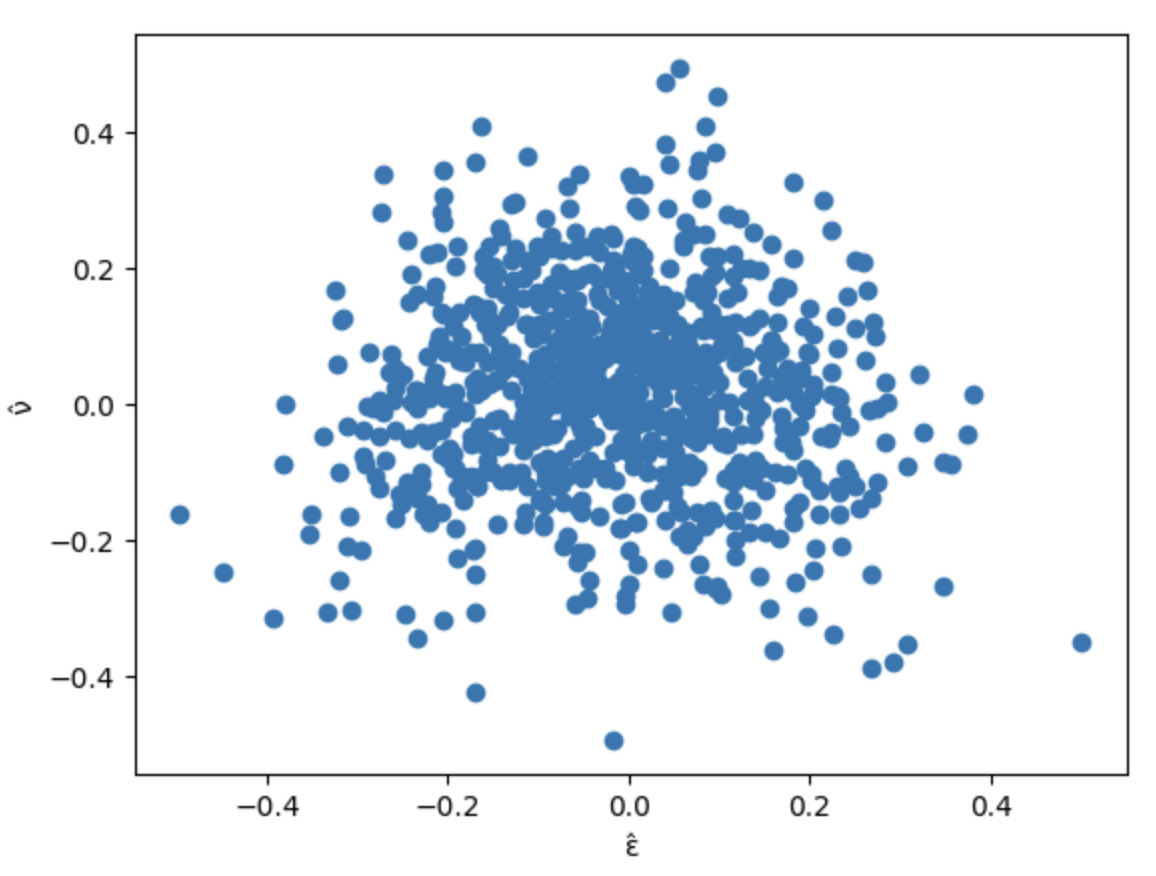
\includegraphics[
            width=\linewidth,
            alt={Scatter plot of residuals from the testing subset
            D2 under the alternative hypothesis. The residuals show
            a nonlinear relationship between X and Y after
            conditioning on Z, indicating remaining dependence.}
        ]{plots/H1_res.png}
        \label{fig:H1-residuals}
    \end{minipage}
    \hfill
    %
    % Right panel: DeepBET representation
    \begin{minipage}{0.45\textwidth}
        \centering
        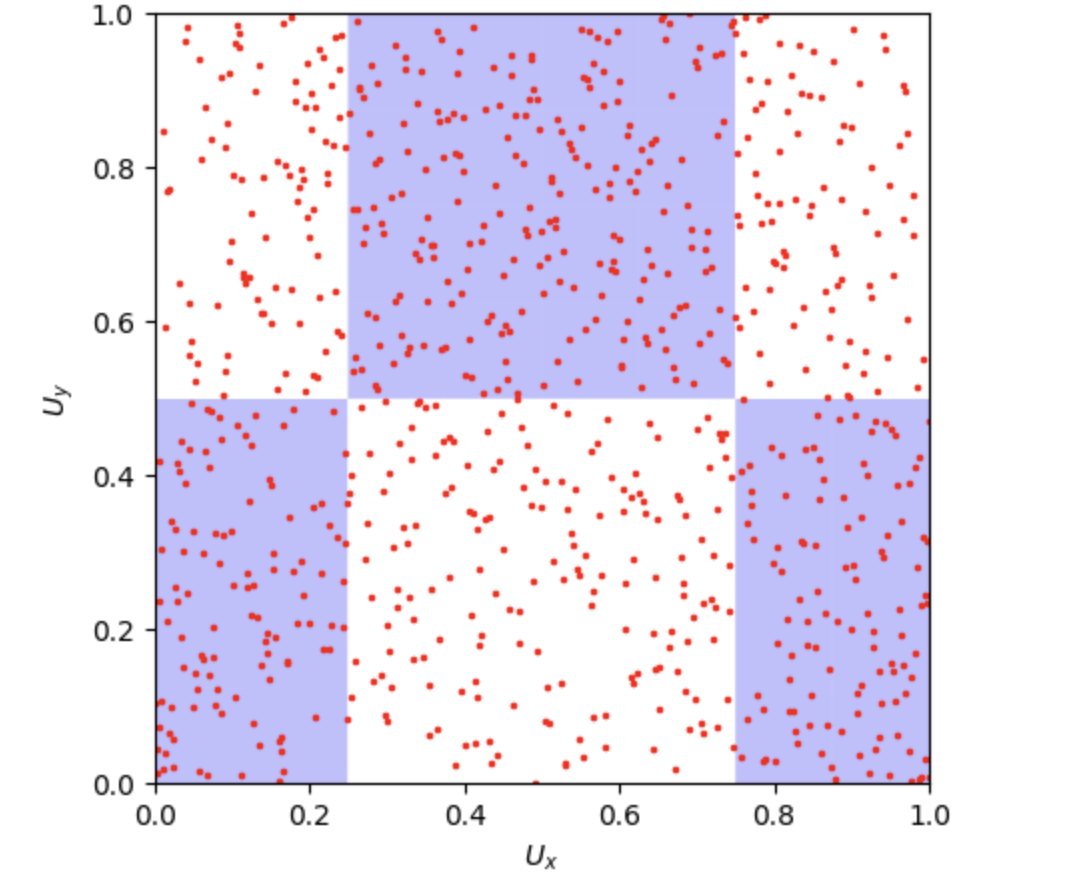
\includegraphics[
            width=\linewidth,
            alt={BET representation of the residuals under the
            alternative hypothesis. The distribution of observations
            is nonuniform across the binary expansion regions,
            indicating dependence involving the first binary expansion
            bit of the Y residuals and the first two binary expansion
            bits of the X residuals.}
        ]{plots/H1_DeepBET.png}
        \label{fig:H1-deepbet}
    \end{minipage}

    \caption{Left: Residuals from the testing subset $\mathcal{D}_2$,
    illustrating the nonlinear relationship between $X$ and $Y$ after
    conditioning on $Z$. Right: The corresponding BET plot reveals a
    noticeably higher density of observations in the highlighted regions,
    indicating dependence driven by the interaction between the first
    binary expansion bit of the $Y$ residuals and the first two binary
    expansion bits of the $X$ residuals.}

    \label{fig:H1-residual-deepbet}
\end{figure}

\hspace{0.5cm}
The BET plot not only supports the detection of conditional dependence but also helps visualize its nonlinear structure. In this example, the higher concentration of points in the blue region relative to the white region indicates a systematic conditional association between $X$ and $Y$ after adjusting for $Z$. Thus, DeepBET provides both a formal test of conditional independence and an interpretable graphical summary of the detected dependence.

\hspace{0.5cm}
The following theorem characterizes the asymptotic null distribution of the proposed BET statistic $\hat{S}_{(\mathbf{ab}),n}$.

\begin{theorem}
\label{thm1}
Suppose that the regression functions $h(\cdot)$ and $g(\cdot)$ are $(p,C)$-smooth generalized hierarchical models of order $d_*$, as defined in Section~\ref{tech_proof}. Assume that the regularity conditions stated in Lemma~\ref{lemma1} are satisfied, and that the cumulative distribution functions $F(\cdot)$ and $G(\cdot)$ possess bounded derivatives. If
\[
d_1=o\!\left(n^{p/(2p+d_*)}\right)
\quad\text{and}\quad
d_2=o\!\left(n^{p/(2p+d_*)}\right),
\]
then, for any $\mathbf{a}\neq0$ and $\mathbf{b}\neq0$,
\[
\frac{\hat{S}_{(\mathbf{ab}),n}+n_{\mathcal{D}_2}}{4}
\]
and
\[
\mathrm{Hypergeometric}\!\left(n_{\mathcal{D}_2},
\frac{n_{\mathcal{D}_2}}{2},
\frac{n_{\mathcal{D}_2}}{2}\right)
\]
converge to the same limiting distribution, where $n_{\mathcal{D}_2}$ denotes the sample size of $\mathcal{D}_2$.
\end{theorem}

\hspace{0.5cm}
Theorem \ref{thm1} provides theoretical support for incorporating DNN estimators into the DeepBET procedure. Because the regression functions are estimated nonparametrically and the covariates $Z$ may be high-dimensional, the convergence rates of the DNN estimators are generally slower than $n^{-1/2}$. Nevertheless, the BET statistic $S_{(\mathbf{ab}),n}$ retains a root-$n$ asymptotic behavior. This is largely due to the binary structure of the transformed variables $\hat{\mathcal{A}}_i$ and $\hat{\mathcal{B}}_i$.

\hspace{0.5cm}
This requirement is weaker than the conditions imposed by several sampling-based conditional independence tests. As a comparison, the generative conditional independence test (GCIT) proposed by \cite{bellot2019conditional} assumes that the total variation distance between the estimated and true conditional distributions converges at a rate faster than $n^{-1/2}$. The double-GAN conditional independence test (DGCIT) of \cite{shi2021double} relaxes this assumption by requiring the product of two total variation distances, corresponding to the conditional distributions of $X\mid Z$ and $Y\mid Z$, to be of smaller order than $n^{-1/2}$. Such assumptions can be difficult to satisfy when the intrinsic dimension $d_*$ in Theorem \ref{thm1} is large and no additional smoothness or sparsity structure is imposed on the regression functions. See \cite{Shah_2020} for further discussion of the challenges associated with nonparametric estimation in high-dimensional conditional independence testing.

\hspace{0.5cm}
Theorem \ref{thm1} implies that
$(n_{\mathcal{D}_2}-1)^{1/2}\hat{S}_{(\mathbf{a}\mathbf{b}),n}/n_{\mathcal{D}_2}$
is asymptotically normal. To improve power across multiple binary interactions, we define the maximal normalized BET statistic as
\begin{center}
    $T_{n} = \max\limits_{\mathbf{ab}\in\sigma(\hat{U}_{d_1}, \hat{V}_{d_2}),\mathbf{a}\neq 0, \mathbf{b}\neq 0}(n_{\mathcal{D}_2}-1)^{1/2}\hat{S}_{(\mathbf{a}\mathbf{b}),n}/n_{\mathcal{D}_2}$. 
\end{center}

\begin{theorem}
\label{thm2}
Suppose that the assumptions of Theorem~\ref{thm1} are satisfied and that
\[
d_1+d_2=o\{\log_2(n^{p/(2p+d_*)})\}.
\]
Then, under the null hypothesis $H_0$, the statistic $\hat{T}_n$ converges in distribution to the maximum of a Gaussian random vector with mean zero and identity covariance matrix as $n\rightarrow\infty$.
\end{theorem}

The proof of Theorem~\ref{thm2} is provided in the Appendix.

\subsection{Multiple Data Splitting with Rank-Transformed Subsampling}

Although the single-split version of DeepBET is easy to implement and computationally attractive, it has several practical limitations. First, the resulting test statistic may vary across different random partitions of the same dataset, introducing additional variability. Second, because only one data split is used to construct the test statistic, the available information is not fully utilized, which may reduce statistical power. First, the resulting test statistic may vary across different random partitions of the data, introducing additional sampling variability. Second, because only a subset of the observations is used to construct the test statistic after model fitting, valuable information from the remaining observations is discarded, which may reduce statistical power. To overcome these limitations, we adopt the multiple-splitting framework proposed by \cite{guo2024ranktransformed}. By combining results from multiple random splits, the procedure reduces split-induced variability while making more effective use of the available data.

\subsubsection{Setup}

Suppose that $T_n^{(1)},\ldots,T_n^{(L)}$ are test statistics computed from $L$ different random splits of the testing sample $\mathcal{D}_2$, where $L$ is specified in advance. We aggregate these statistics through
\begin{center}
    $\Lambda_n = ( |T_n^{(1)}|+\cdots+|T_n^{(L)}| )/L,$
\end{center}
where $T_n^{(l)}$ denotes the BET statistic corresponding to the $l$-th sample split for $l=1,\ldots,L$. When $L$ is sufficiently large, the conditional variance
$\mathrm{Var}(\Lambda_n \mid X_1,\ldots,X_n)$
becomes small, so that the aggregated statistic is substantially less sensitive to the randomness introduced by data splitting.

\hspace{0.5cm}
By Theorem \ref{thm2}, the aggregated statistic $\Lambda_n$ converges in distribution to a limiting distribution $G_p$ under the null hypothesis. Consequently, the null hypothesis is rejected for sufficiently large values of $\Lambda_n$. Ideally, one would compare $\Lambda_n$ with the unknown upper $\alpha$-quantile of $G_p$. Since this limiting distribution is unavailable in practice, we approximate it using a rank-transformed subsampling procedure. The resulting empirical distribution, denoted by $\tilde{G}_n$, is then used to estimate the critical value for the proposed test.

\subsubsection{Rank-transformed subsampling}

We now describe the rank-transformed subsampling procedure for a single aggregation function $\Lambda_n$.

\hspace{0.5cm}
\textbf{Subsampling.}
Let $m<n$ denote the subsample size. Throughout the numerical studies in this chapter, we choose
\[
m=\left[\frac{n}{\log n}\right].
\]
A total of $B$ subsamples, each containing $m$ observations, are generated with only limited overlap between different subsamples. Specifically, let $J$ denote a positive integer (for example, $J=50$), and set
\[
B=J[n/m].
\]
The corresponding collection of subsample index sets is
\[
\mathcal{B}
=
\{(i_{1,b},\ldots,i_{m,b}):b=1,\ldots,B\},
\]
which is constructed according to Algorithm~\ref{alg:subsampling} described in \cite{guo2024ranktransformed}.

% ============================================================
% Construction of subsample index tuples
% Accessible EPUB version + original PDF version
% ============================================================

\iflatexml

\noindent
\textbf{Algorithm: Construction of subsample index tuples}

\begin{enumerate}

    \item \textbf{Input:}
    Sample size $n$, subsample size $m$, and positive integer $J$.

    \item Initialize
    \[
    \mathcal{B}\gets\emptyset.
    \]

    \item For $j=1,\ldots,J$, perform the following steps:
    \begin{enumerate}

        \item Generate a random permutation
        \[
        \pi=(\pi_1,\ldots,\pi_n)
        \]
        of $\{1,\ldots,n\}$.

        \item Add the nonoverlapping subsample index tuples of
        size $m$ to $\mathcal{B}$:
        \[
        \mathcal{B}\gets \mathcal{B}\cup
        \left\{
        (\pi_1,\ldots,\pi_m),
        (\pi_{m+1},\ldots,\pi_{2m}),
        \ldots,
        (\pi_{(\lfloor n/m\rfloor-1)m+1},
        \ldots,
        \pi_{\lfloor n/m\rfloor m})
        \right\}.
        \]

    \end{enumerate}

    \item \textbf{Return} $\mathcal{B}$.

\end{enumerate}

\else

\begin{algorithm}[htbp!]
\caption{Construction of subsample index tuples}
\label{alg:subsampling}

\begin{algorithmic}[1]

\State \textbf{Input:} Sample size $n$, subsample size $m$,
and positive integer $J$

\State $\mathcal{B}\gets\emptyset$

\For{$j=1,\ldots,J$}

    \State Generate a random permutation
    $\pi=(\pi_1,\ldots,\pi_n)$
    of $\{1,\ldots,n\}$

    \State $\mathcal{B}\gets \mathcal{B}\cup
    \{(\pi_1,\ldots,\pi_m),
    (\pi_{m+1},\ldots,\pi_{2m}),
    \ldots,
    (\pi_{(\lfloor n/m\rfloor-1)m+1},
    \ldots,
    \pi_{\lfloor n/m\rfloor m})\}$

\EndFor

\State \textbf{return} $\mathcal{B}$

\end{algorithmic}
\end{algorithm}

\fi


% ============================================================
% Subsampling distribution
% ============================================================

For each subsample, the corresponding test statistics are arranged into a
$B\times L$ matrix
\[
\widehat{H}=(\widehat{H}_{b,l}),
\]
whose $b$-th row is given by
\[
\widehat{H}_{b,\cdot}
:=
\left(
T_m^{(1)}(X_{{i}_{1,b}},\ldots,X_{{i}_{m,b}}),
\ldots,
T_m^{(L)}(X_{{i}_{1,b}},\ldots,X_{{i}_{m,b}})
\right),
\qquad b=1,\ldots,B.
\]

Applying the aggregation function to each row yields
\[
\widehat{\Lambda}_{b}
=
\Lambda_n(\widehat{H}_{b,1},\ldots,\widehat{H}_{b,L}),
\]
whose empirical distribution function
\[
\widehat{G}_n(x)
=
\mathbb{F}_{\{\widehat{\Lambda}_b\}}(x)
\]
provides a natural subsampling approximation to the limiting distribution
$G_p(x)$.


% ============================================================
% Rank transformation
% ============================================================

\medskip
\noindent
\textbf{Rank transformation.}
Let $\mathbb{F}_{\widehat{H}}$ denote the empirical distribution function
of all entries in $\widehat{H}$. We transform each entry according to
\[
\tilde{H}_{b,l}
=
F_0^{-1}
\left\{
\frac{R_{b,l}-1/2}{BL}
\right\},
\]
where $R_{b,l}$ denotes the rank of
$T_m^{(l)}(\mathcal{D}_2^{(b)})$
among all
$\{T_m^{(l)}(\mathcal{D}_2^{(b)})\}$
for $b=1,\ldots,B$ and $l=1,\ldots,L$, and $F_0$ is the cumulative
distribution function of the standard normal distribution.

The transformed statistics are then aggregated as
\[
\tilde{\Lambda}_{b}
:=
\Lambda_n(
\tilde{H}_{b,1},
\ldots,
\tilde{H}_{b,L}
),
\]
and their empirical distribution
\[
\tilde{G}_n(x)
=
\mathbb{F}_{\{\tilde{\Lambda}_b\}}(x)
\]
is used to estimate the critical value
$\tilde{G}_n^{-1}(1-\alpha)$
for the aggregated statistic $\Lambda_n$.

The complete multiple-splitting procedure is summarized in
Algorithm~\ref{alg:multiple-split}.

% ============================================================
% Rank-transformed aggregated multiple-split test
% Accessible EPUB version + original PDF version
% ============================================================

\iflatexml

\refstepcounter{algorithm}
\label{alg:multiple-split}

\noindent
\textbf{Algorithm \thealgorithm: Rank-transformed aggregated
multiple-split test}

\begin{enumerate}

    \item \textbf{Input:}
    Observations $X_1,\ldots,X_n$;
    exchangeable single-split statistics
    $T_n^{(1)},\ldots,T_n^{(L)}$;
    limiting null CDF $F_0$;
    aggregation rule $\Lambda_n$;
    significance level $\alpha\in(0,1)$;
    and positive integer $J$.

    \item Set
    \[
    m\gets \left\lfloor \frac{n}{\log n}\right\rfloor,
    \qquad
    B\gets J\left\lfloor \frac{n}{m}\right\rfloor.
    \]

    \item Generate the subsample index collection
    \[
    \mathcal{B}
    =
    \left\{
    (i_{1,b},\ldots,i_{m,b})
    :
    b=1,\ldots,B
    \right\}
    \]
    using Algorithm~\ref{alg:subsampling}.

    \item Initialize the $B\times L$ matrices
    $\widehat{H}$ and $\widetilde{H}$,
    together with
    \[
    \widetilde{\Lambda}\in\mathbb{R}^{B}.
    \]

    \item For each $b=1,\ldots,B$, compute
    \[
    \widehat{H}_{b,\cdot}
    \gets
    \left(
    T_m^{(1)}(X_{i_{1,b}},\ldots,X_{i_{m,b}}),
    \ldots,
    T_m^{(L)}(X_{i_{1,b}},\ldots,X_{i_{m,b}})
    \right).
    \]

    \item For each $b=1,\ldots,B$, perform the following:

    \begin{enumerate}

        \item For each $l=1,\ldots,L$, set
        \[
        \widetilde{H}_{b,l}
        \gets
        F_0^{-1}
        \left\{
        \frac{R_{b,l}-1/2}{BL}
        \right\}.
        \]

        \item Aggregate the transformed statistics:
        \[
        \widetilde{\Lambda}_b
        \gets
        \Lambda_n
        \left(
        |\widetilde{H}_{b,1}|,
        \ldots,
        |\widetilde{H}_{b,L}|
        \right).
        \]

    \end{enumerate}

    \item Define the empirical distribution
    \[
    \widetilde{G}_n
    \gets
    \mathbb{F}_{
    \{\widetilde{\Lambda}_b:
    b=1,\ldots,B\}
    }.
    \]

    \item Using the full sample
    $X_1,\ldots,X_n$, compute
    \[
    \Lambda_n
    \gets
    \Lambda_n
    \left(
    |T_n^{(1)}|,
    \ldots,
    |T_n^{(L)}|
    \right).
    \]

    \item \textbf{Decision:}
    Reject $H_0$ if
    \[
    \Lambda_n
    >
    \widetilde{G}_n^{-1}(1-\alpha/2).
    \]
    Report the p-value
    \[
    1-\widetilde{G}_n(\Lambda_n).
    \]

\end{enumerate}

\else

\begin{algorithm}[htbp!]
\caption{Rank-transformed aggregated multiple-split test}
\label{alg:multiple-split}

\begin{algorithmic}[1]

\State \textbf{Input:} Observations $X_1,\ldots,X_n$;
exchangeable single-split statistics
$T_n^{(1)},\ldots,T_n^{(L)}$;
limiting null CDF $F_0$;
aggregation rule $\Lambda_n$;
significance level $\alpha\in(0,1)$;
positive integer $J$

\State Set
$m\gets \lfloor n/\log n\rfloor$
and
$B\gets J\lfloor n/m\rfloor$

\State Generate the subsample index collection
$\mathcal{B}
=
\{(i_{1,b},\ldots,i_{m,b}):
b=1,\ldots,B\}$
using Algorithm~\ref{alg:subsampling}

\State Initialize $B\times L$ matrices
$\widehat{H}$ and $\widetilde{H}$,
together with a vector
$\widetilde{\Lambda}\in\mathbb{R}^{B}$

\For{$b=1,\ldots,B$}

    \State
    $\widehat{H}_{b,\cdot}\gets
    \big(
    T_m^{(1)}(X_{i_{1,b}},\ldots,X_{i_{m,b}}),
    \ldots,
    T_m^{(L)}(X_{i_{1,b}},\ldots,X_{i_{m,b}})
    \big)$

\EndFor

\For{$b=1,\ldots,B$}

    \For{$l=1,\ldots,L$}

        \State
        $\widetilde{H}_{b,l}
        \gets
        F_0^{-1}
        \{(R_{b,l}-1/2)/(BL)\}$

    \EndFor

    \State
    $\widetilde{\Lambda}_b
    \gets
    \Lambda_n(
    |\widetilde{H}_{b,1}|,
    \ldots,
    |\widetilde{H}_{b,L}|
    )$

\EndFor

\State Define
$\widetilde{G}_n
\gets
\mathbb{F}_{
\{\widetilde{\Lambda}_b:
b=1,\ldots,B\}
}$

\State Compute the full-sample statistic
$\Lambda_n
\gets
\Lambda_n(
|T_n^{(1)}|,
\ldots,
|T_n^{(L)}|
)$
using $X_1,\ldots,X_n$

\State Reject $H_0$ if
$\Lambda_n>
\widetilde{G}_n^{-1}(1-\alpha/2)$;
report the p-value
$1-\widetilde{G}_n(\Lambda_n)$

\end{algorithmic}
\end{algorithm}

\fi




\section{Numerical Studies}
\label{Numerical studies}

We first describe the implementation details used in our experiments. We then present simulation studies assessing the empirical size and power of the proposed method and compare its performance with several existing conditional independence tests.

\subsection{Details of Implementing DNN}

The choice of the number of splits $L$ in Algorithm 2 involves a trade-off between statistical power and computational cost. A larger value of $L$ can improve the stability and power of the aggregated test, but it also increases the computational burden. Based on our empirical studies, values of $L$ between 30 and 50 generally provide a good balance. Therefore, throughout the simulations, we set $L=40$.

Existing theoretical results have shown that deep neural networks can consistently estimate nonparametric functions involving high-dimensional covariates and can help mitigate the curse of dimensionality (e.g., \cite{chen1998sieve}; \cite{schmidt2020nonparametric}). However, their use in statistical inference tasks, particularly conditional independence testing, has not been fully explored. For this reason, we carefully tune the DNN component and examine how its tuning parameters affect the proposed test.

In our implementation, we use fully connected neural networks and consider several activation functions, including LeakyReLU, ReLU, and Tanh. The data are divided into training and testing parts with a ratio of $1:4$. The learning rate is set to $0.005$, the batch size is set to $50$, and the number of training epochs is set to $15$. Model parameters are optimized using the Adam optimizer. To reduce overfitting and improve generalization, we apply dropout with rate $0.2$, meaning that 20\% of neurons are randomly dropped in each layer during training.

\subsection{Simulations}
\label{simulation_results}

\subsubsection*{Simulation setting I}

We generate data from a post-nonlinear noise model similar to the simulation settings adopted by \cite{shi2021double} and \cite{bellot2019conditional}. Specifically, the data are generated according to
\begin{center}
$X= \sin(a_f^{T}Z) + \epsilon_f$,\ and \ $ Y= \cos(a_g^{T}Z+ bX)+ \nu_g.$
\end{center}
The coefficient vectors $a_f$ and $a_g$ are independently drawn from the uniform distribution on $[0,1]$ and subsequently rescaled to have unit $\ell_1$ norm. The error terms $\epsilon_f$ and $\nu_g$ are generated independently from a Gaussian distribution with mean $0$ and variance $0.25$. The scalar parameter $b$ governs the degree of conditional dependence between $X$ and $Y$. Under the null hypothesis, $b=0$, whereas nonzero values of $b$ correspond to the alternative hypothesis. Throughout the experiments, the nominal significance level is fixed at $\alpha=0.05$, and all empirical results are obtained from 500 independent Monte Carlo replications.

\hspace{0.5cm}
The left panel of Figure~\ref{fig:BETandGMC DNNand RF} compares the empirical size and power of the proposed DeepBET procedure with the generalized covariance measure (GCM) test \cite{Shah_2020}. Both methods employ residuals estimated by a deep neural network using a single sample split. In this experiment, the confounding dimension is fixed at $d_Z=100$ with sample size $n=1000$, while the dependence parameter $b$ takes values in $\{0,0.45,0.6,0.75,0.9\}$. The results demonstrate that DeepBET consistently provides higher empirical power than the DNN+GCM approach while maintaining appropriate type I error control.

\hspace{0.5cm}
To further evaluate the effect of the regression model used for residual estimation, we compare DeepBET based on deep neural networks with BET using random forest residuals. The right panel of Figure~\ref{fig:BETandGMC DNNand RF} summarizes the empirical size and power for the setting $d_Z=500$ and $n=500$, using the same values of $b$. The results indicate that the DNN-based implementation consistently outperforms the random forest alternative across the range of dependence strengths considered.

\begin{figure}[htbp!]
    \centering
    \begin{minipage}{0.45\textwidth}\
        \centering
        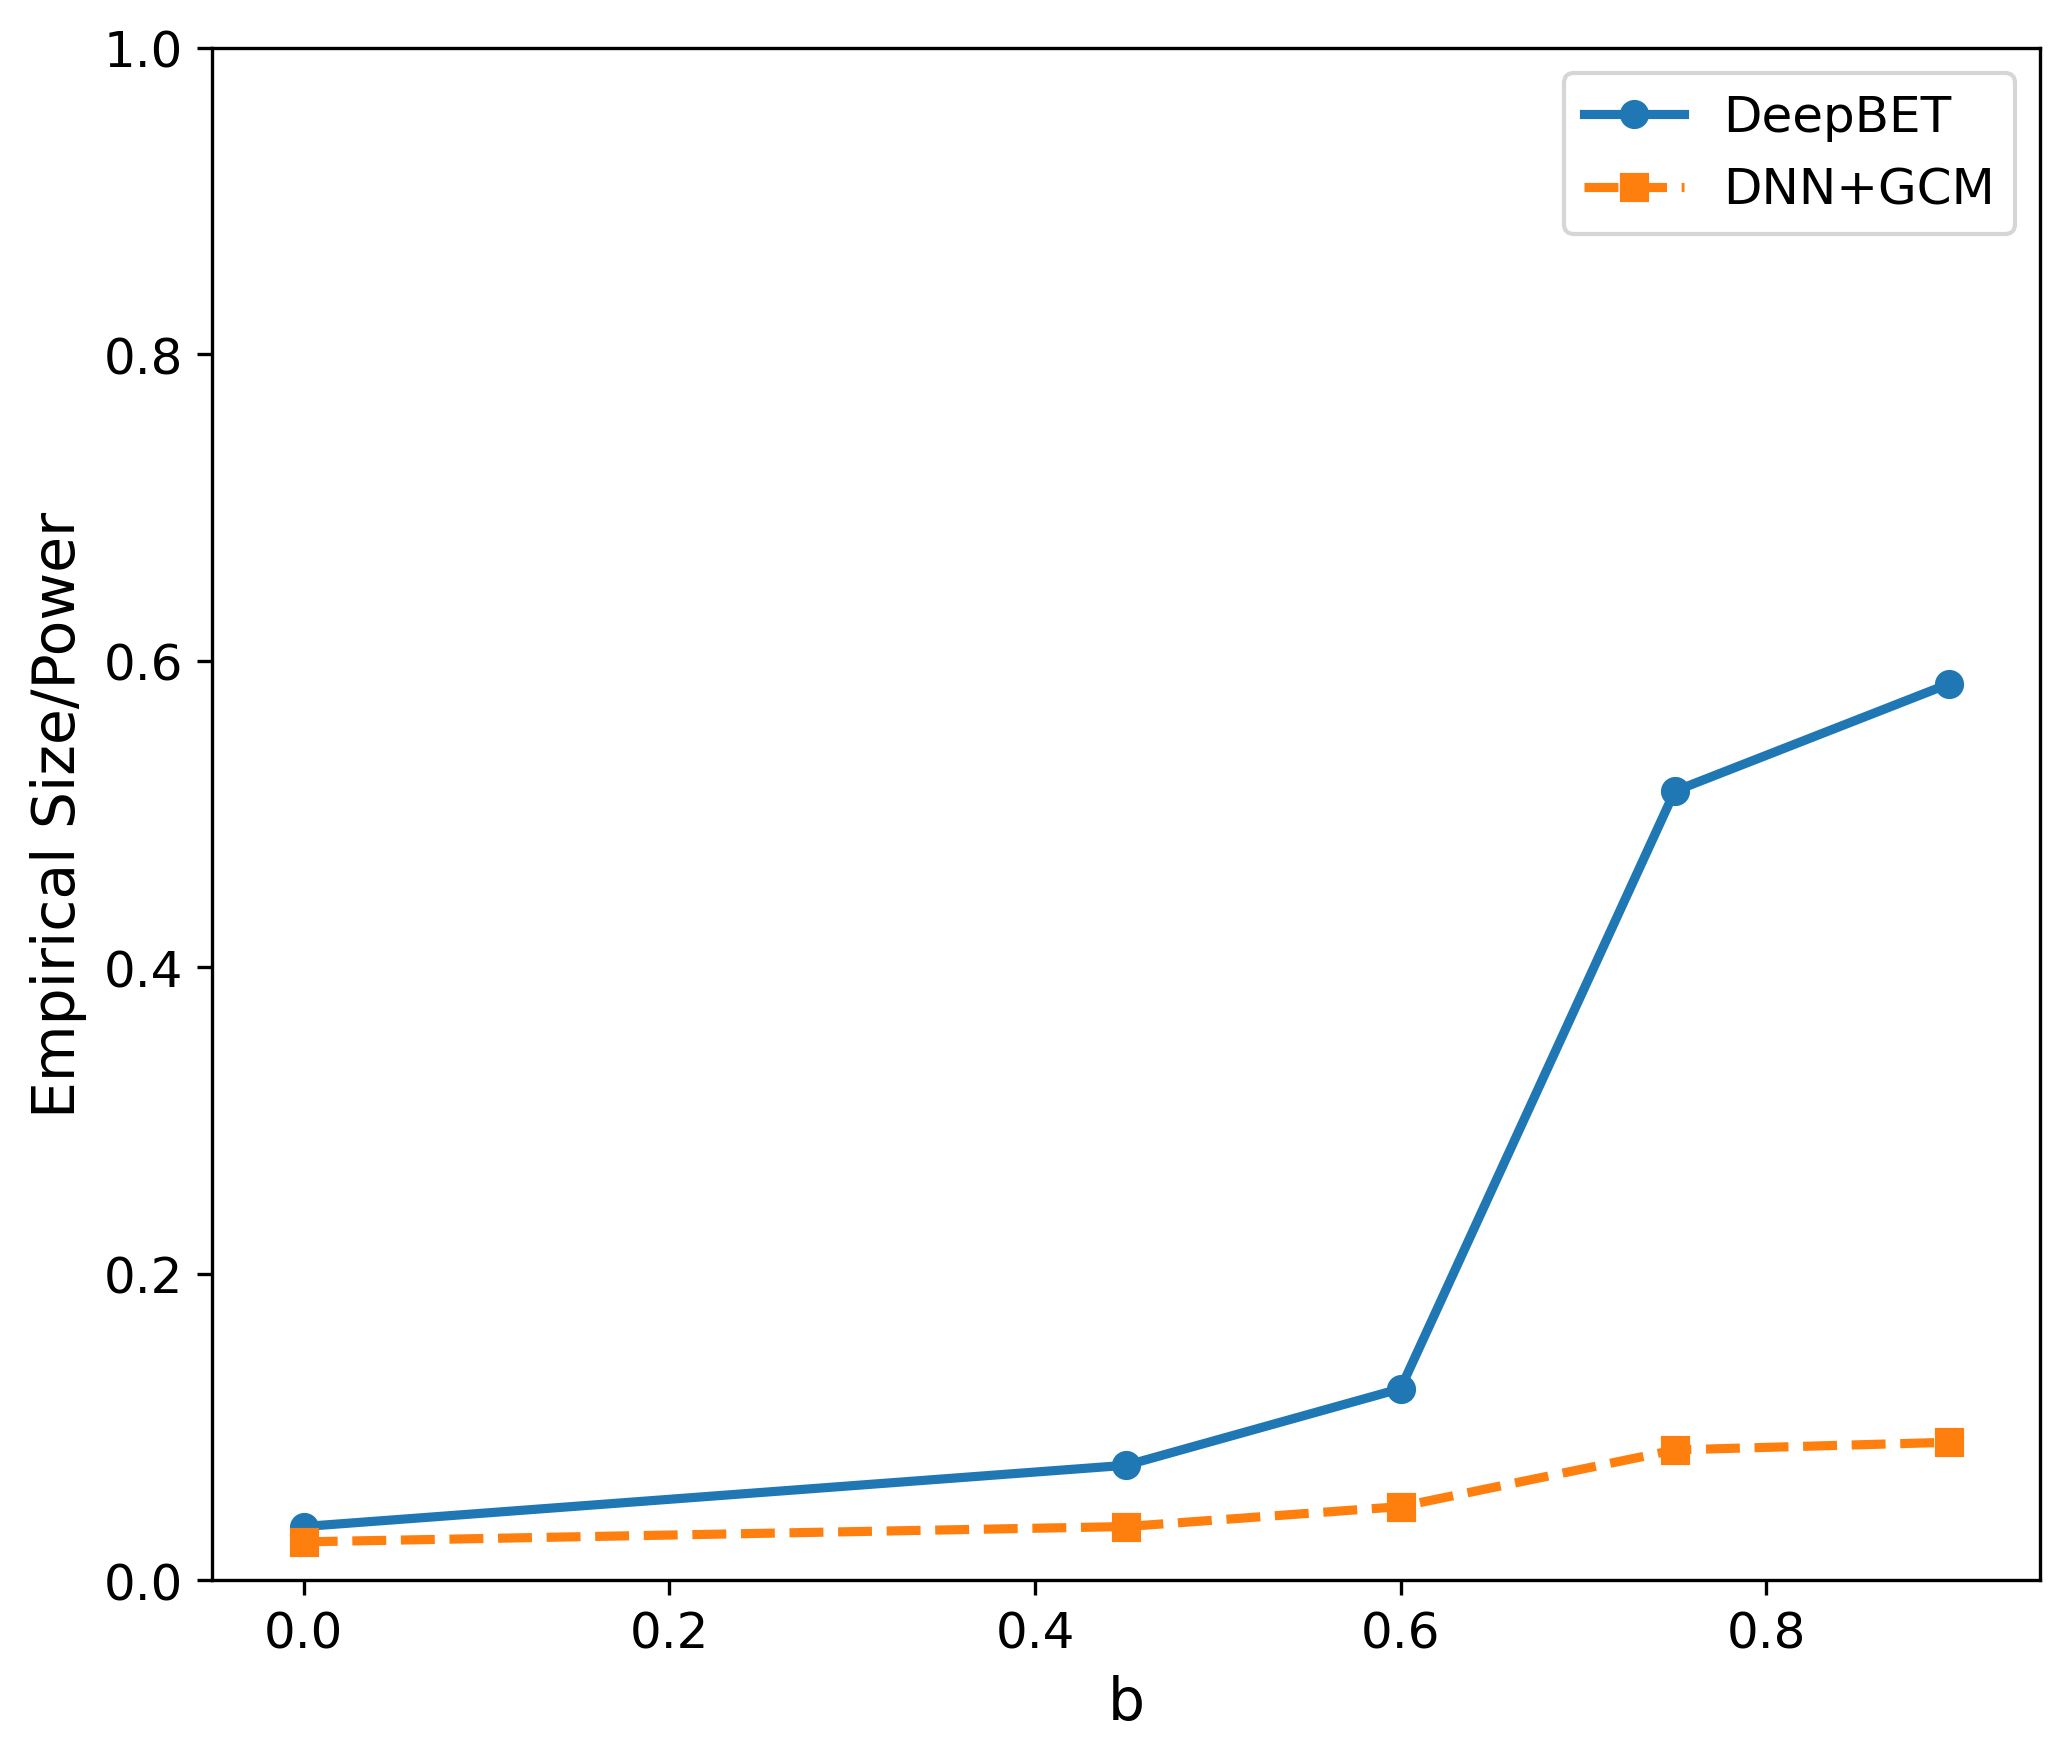
\includegraphics[width=\linewidth, alt={Empirical size and power curves comparing DeepBET and
DNN plus GCM as signal strength b increases. DeepBET shows
substantially greater power at stronger signals.}]{plots/BETvs.GCM.png}
    \end{minipage} 
    \begin{minipage}{0.45\textwidth}
        \centering
        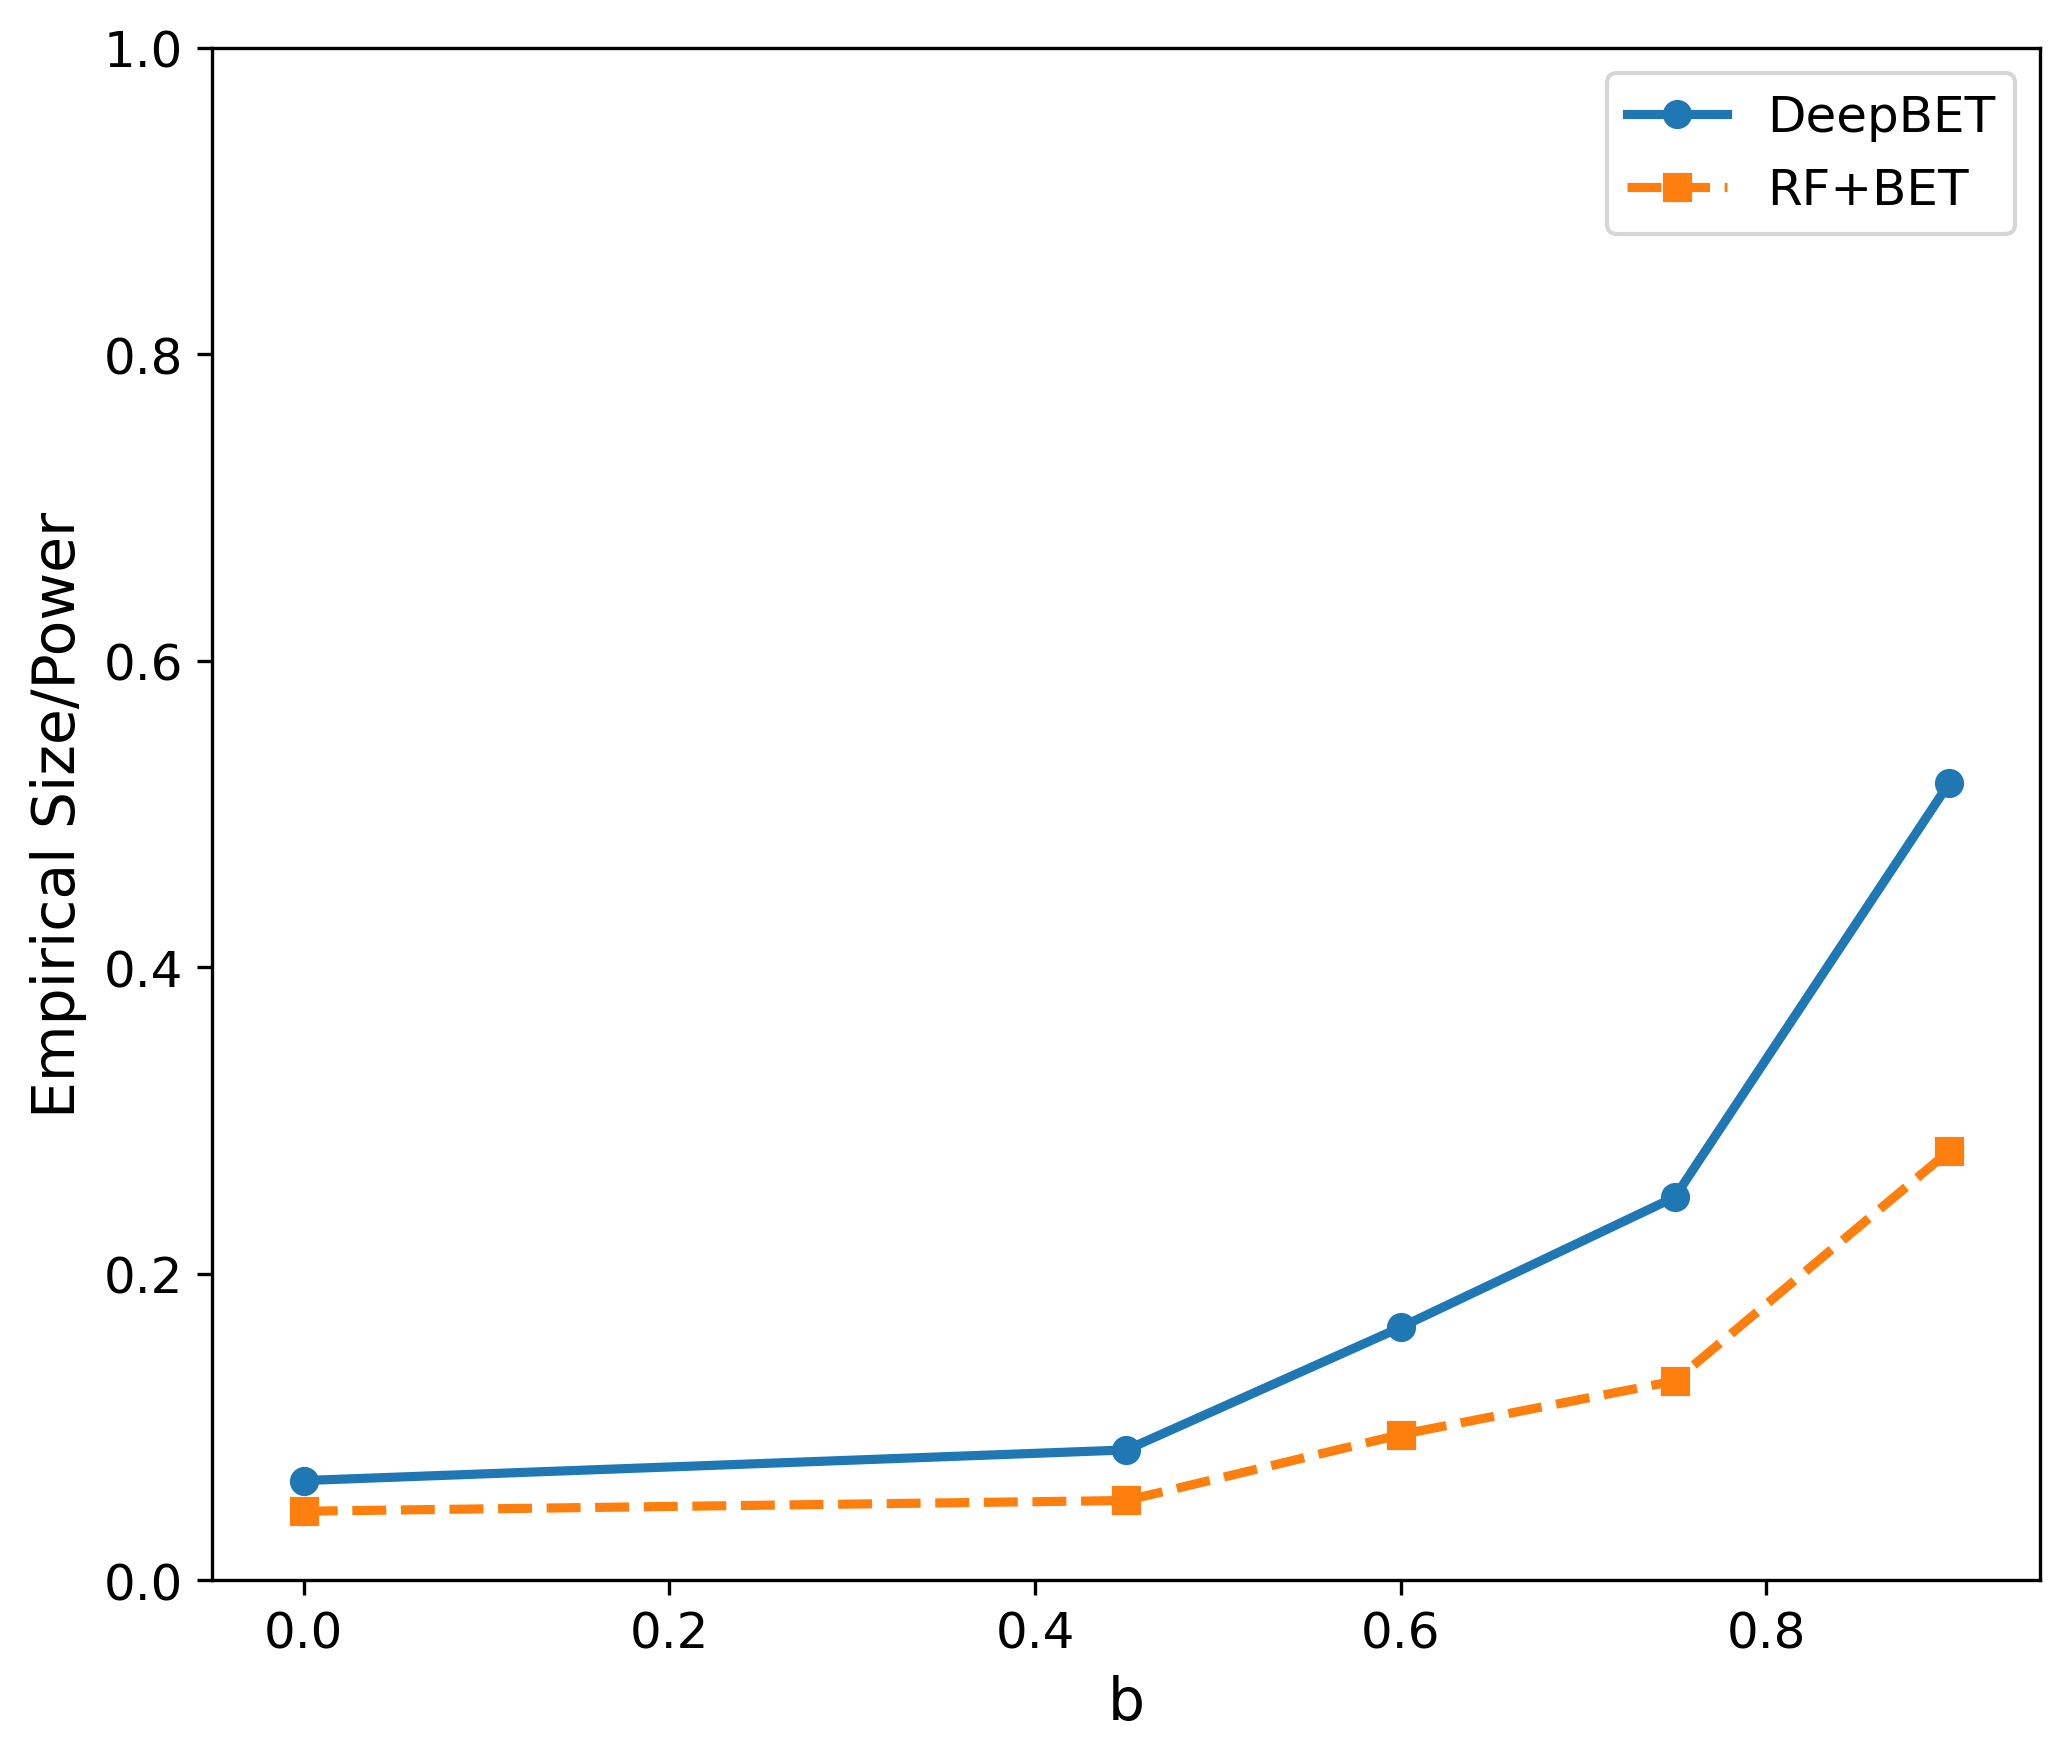
\includegraphics[width=\linewidth, alt={Empirical size and power curves comparing neural-network-based
DeepBET with random-forest-based BET as signal strength increases.}]{plots/DNN and RF.png}
    \end{minipage}
    \caption{Left: Empirical size and power of DeepBET and DNN+GCM. Right: Empirical size and power of DeepBET and RF+BET.}
    \label{fig:BETandGMC DNNand RF}
\end{figure} 

\hspace{0.5cm}
Figure \ref{fig:main} compares the single-split and multiple-split versions of the proposed method. We set $d_Z=100$ and vary $b$ over $0,0.45,0.6,0.75,$ and $0.9$. The multiple-split version controls the type I error while substantially improving power. In particular, when $b$ is close to $0.9$, the power is nearly doubled compared with the single-split version.

\begin{figure}[htbp!]
    \centering
    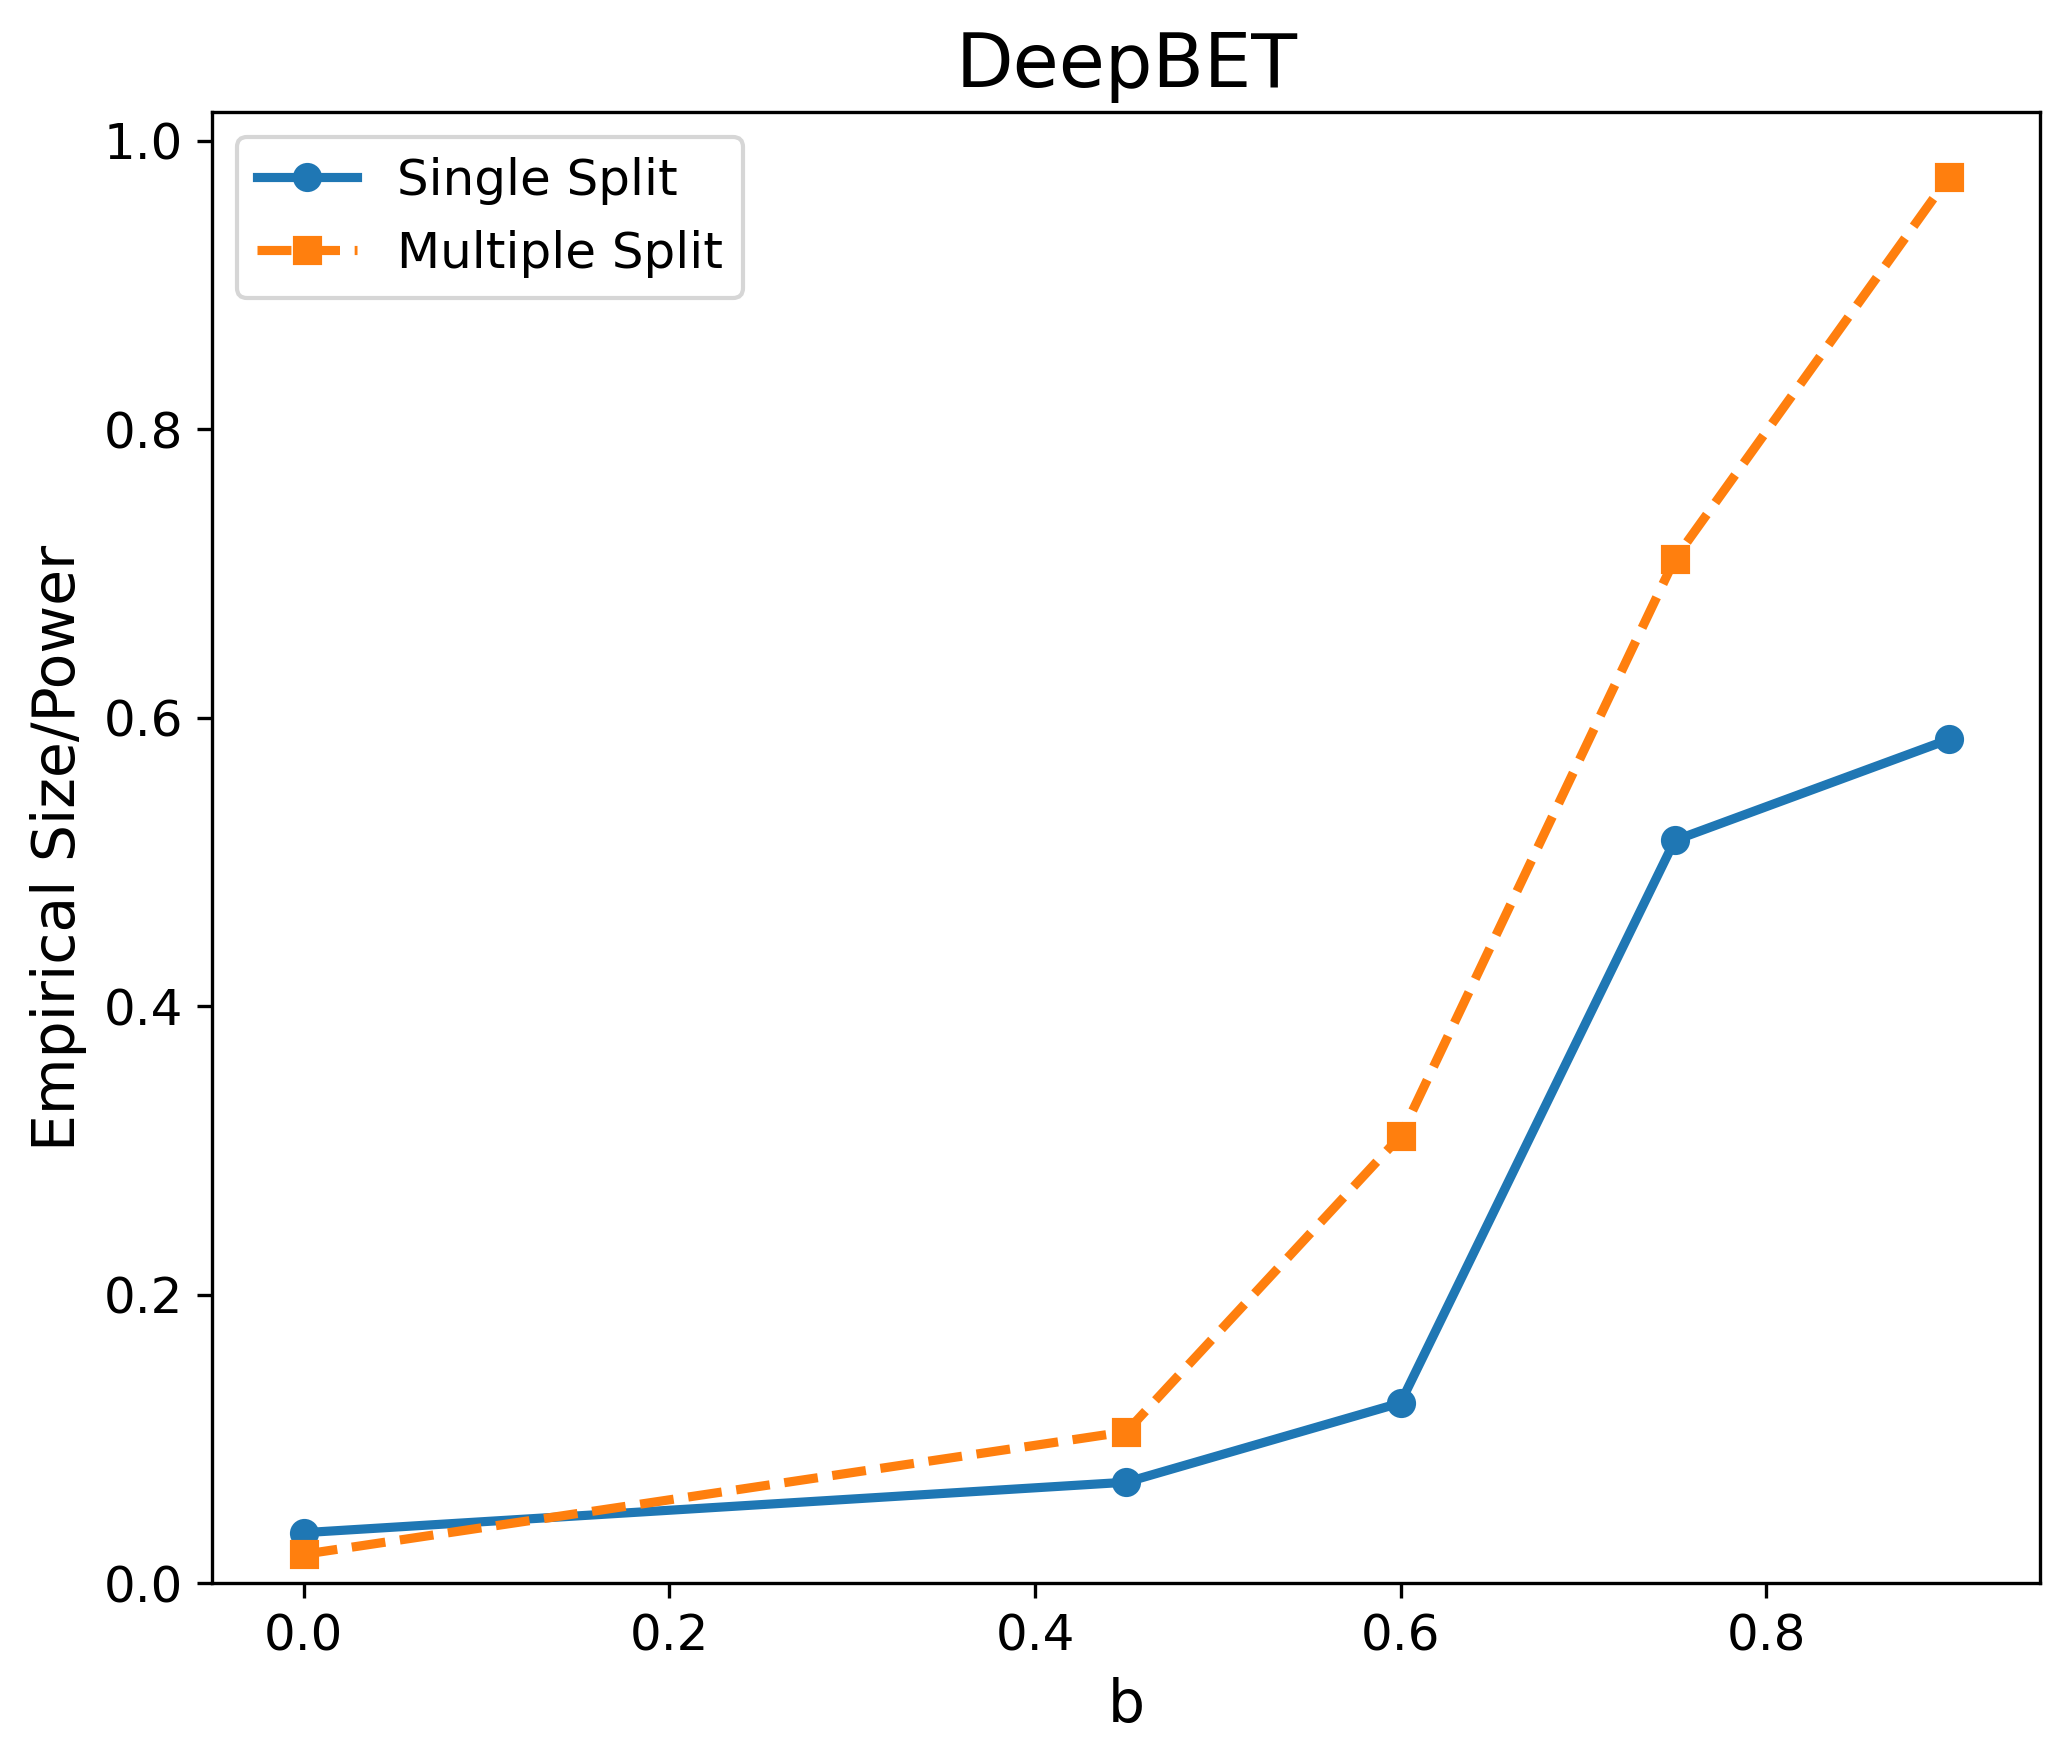
\includegraphics[width=0.45\textwidth, alt={Empirical size and power curves comparing single-split and
multiple-split DeepBET. Multiple splitting provides higher power
as signal strength increases.}]{plots/Single and Multiple split.png} 
    \caption{Empirical size and power of the proposed test using single splitting and multiple splitting.}
    \label{fig:main}
\end{figure}

\hspace{0.5cm}
We next examine whether the activation function used in the DNN has a substantial impact on the performance of DeepBET. To this end, we compare different activation functions under several dimensions of $Z$, namely $d_Z=50,100,150,200,$ and $250$, with $Z$ generated from a standard normal distribution. We also study the empirical power when $d_Z=100$ and $b=0.45,0.6,0.75,$ and $0.9$. As shown in Figure \ref{fig:4}, the empirical results are very similar across activation functions, suggesting that DeepBET is relatively robust to this tuning choice.

\begin{figure}[H]
    \centering
    \begin{minipage}{0.45\textwidth} 
        \centering
        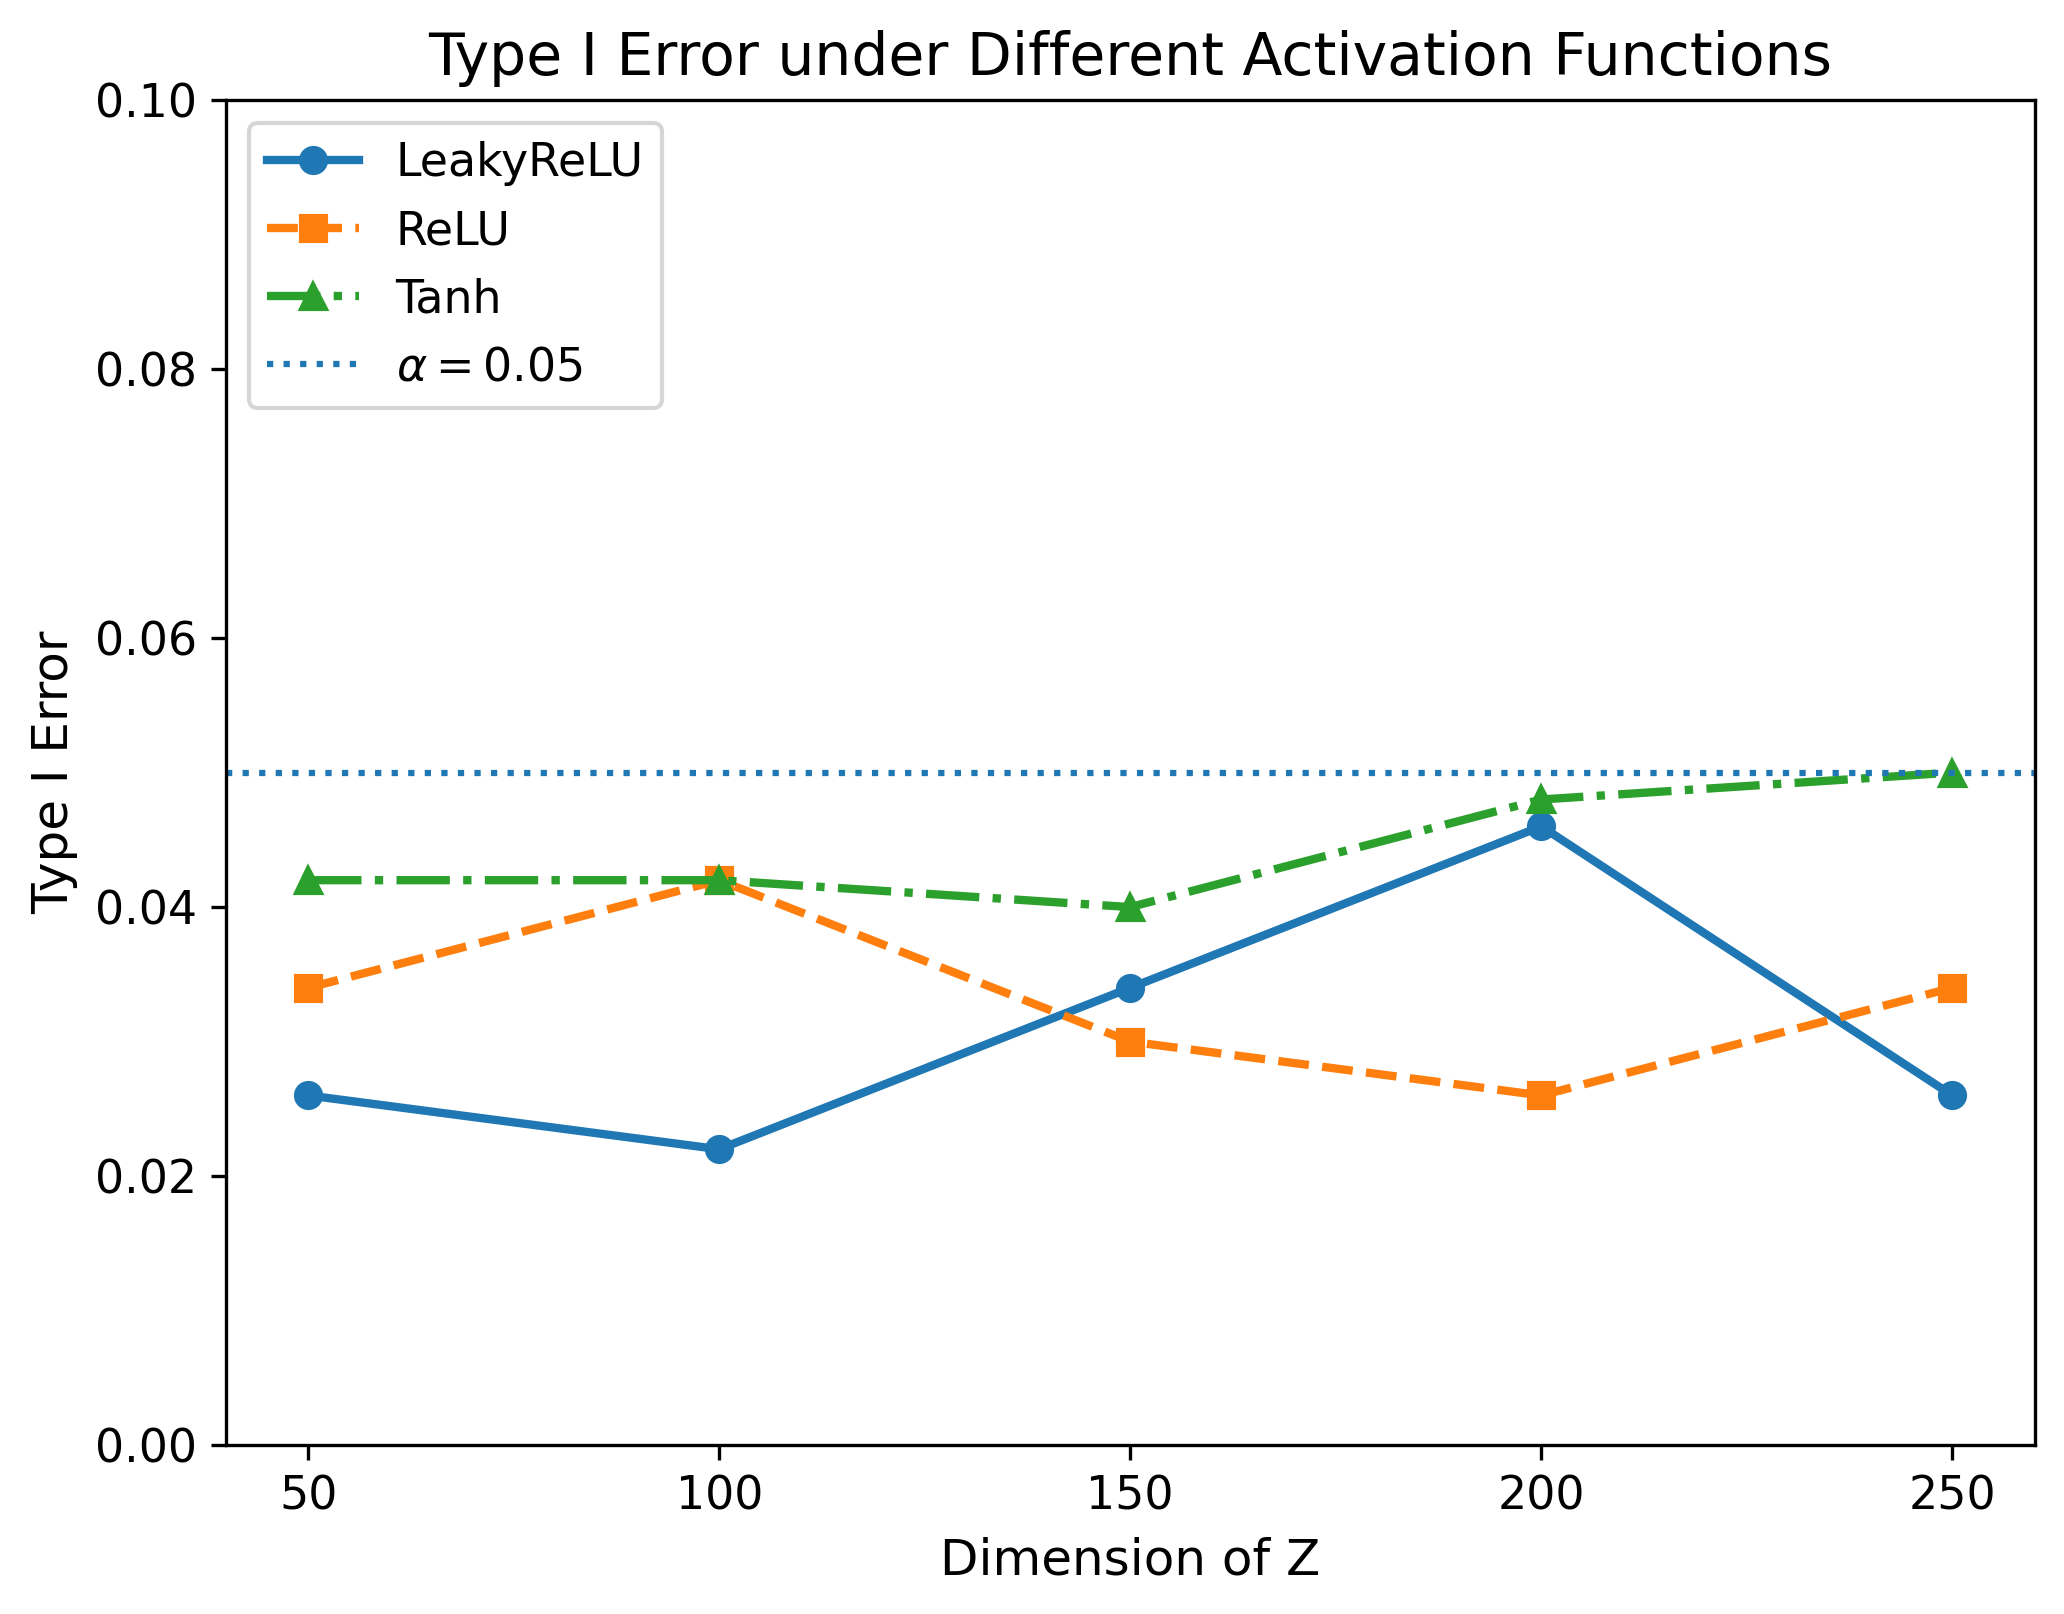
\includegraphics[width=\linewidth, alt={Empirical Type I error of DeepBET using LeakyReLU, ReLU,
and Tanh activation functions across increasing dimensions of Z.
All three activation functions maintain Type I error near the
nominal level.}]{plots/type1error act.png}
        \label{fig:imageA}
    \end{minipage} \hfill
    \begin{minipage}{0.45\textwidth}
        \centering
        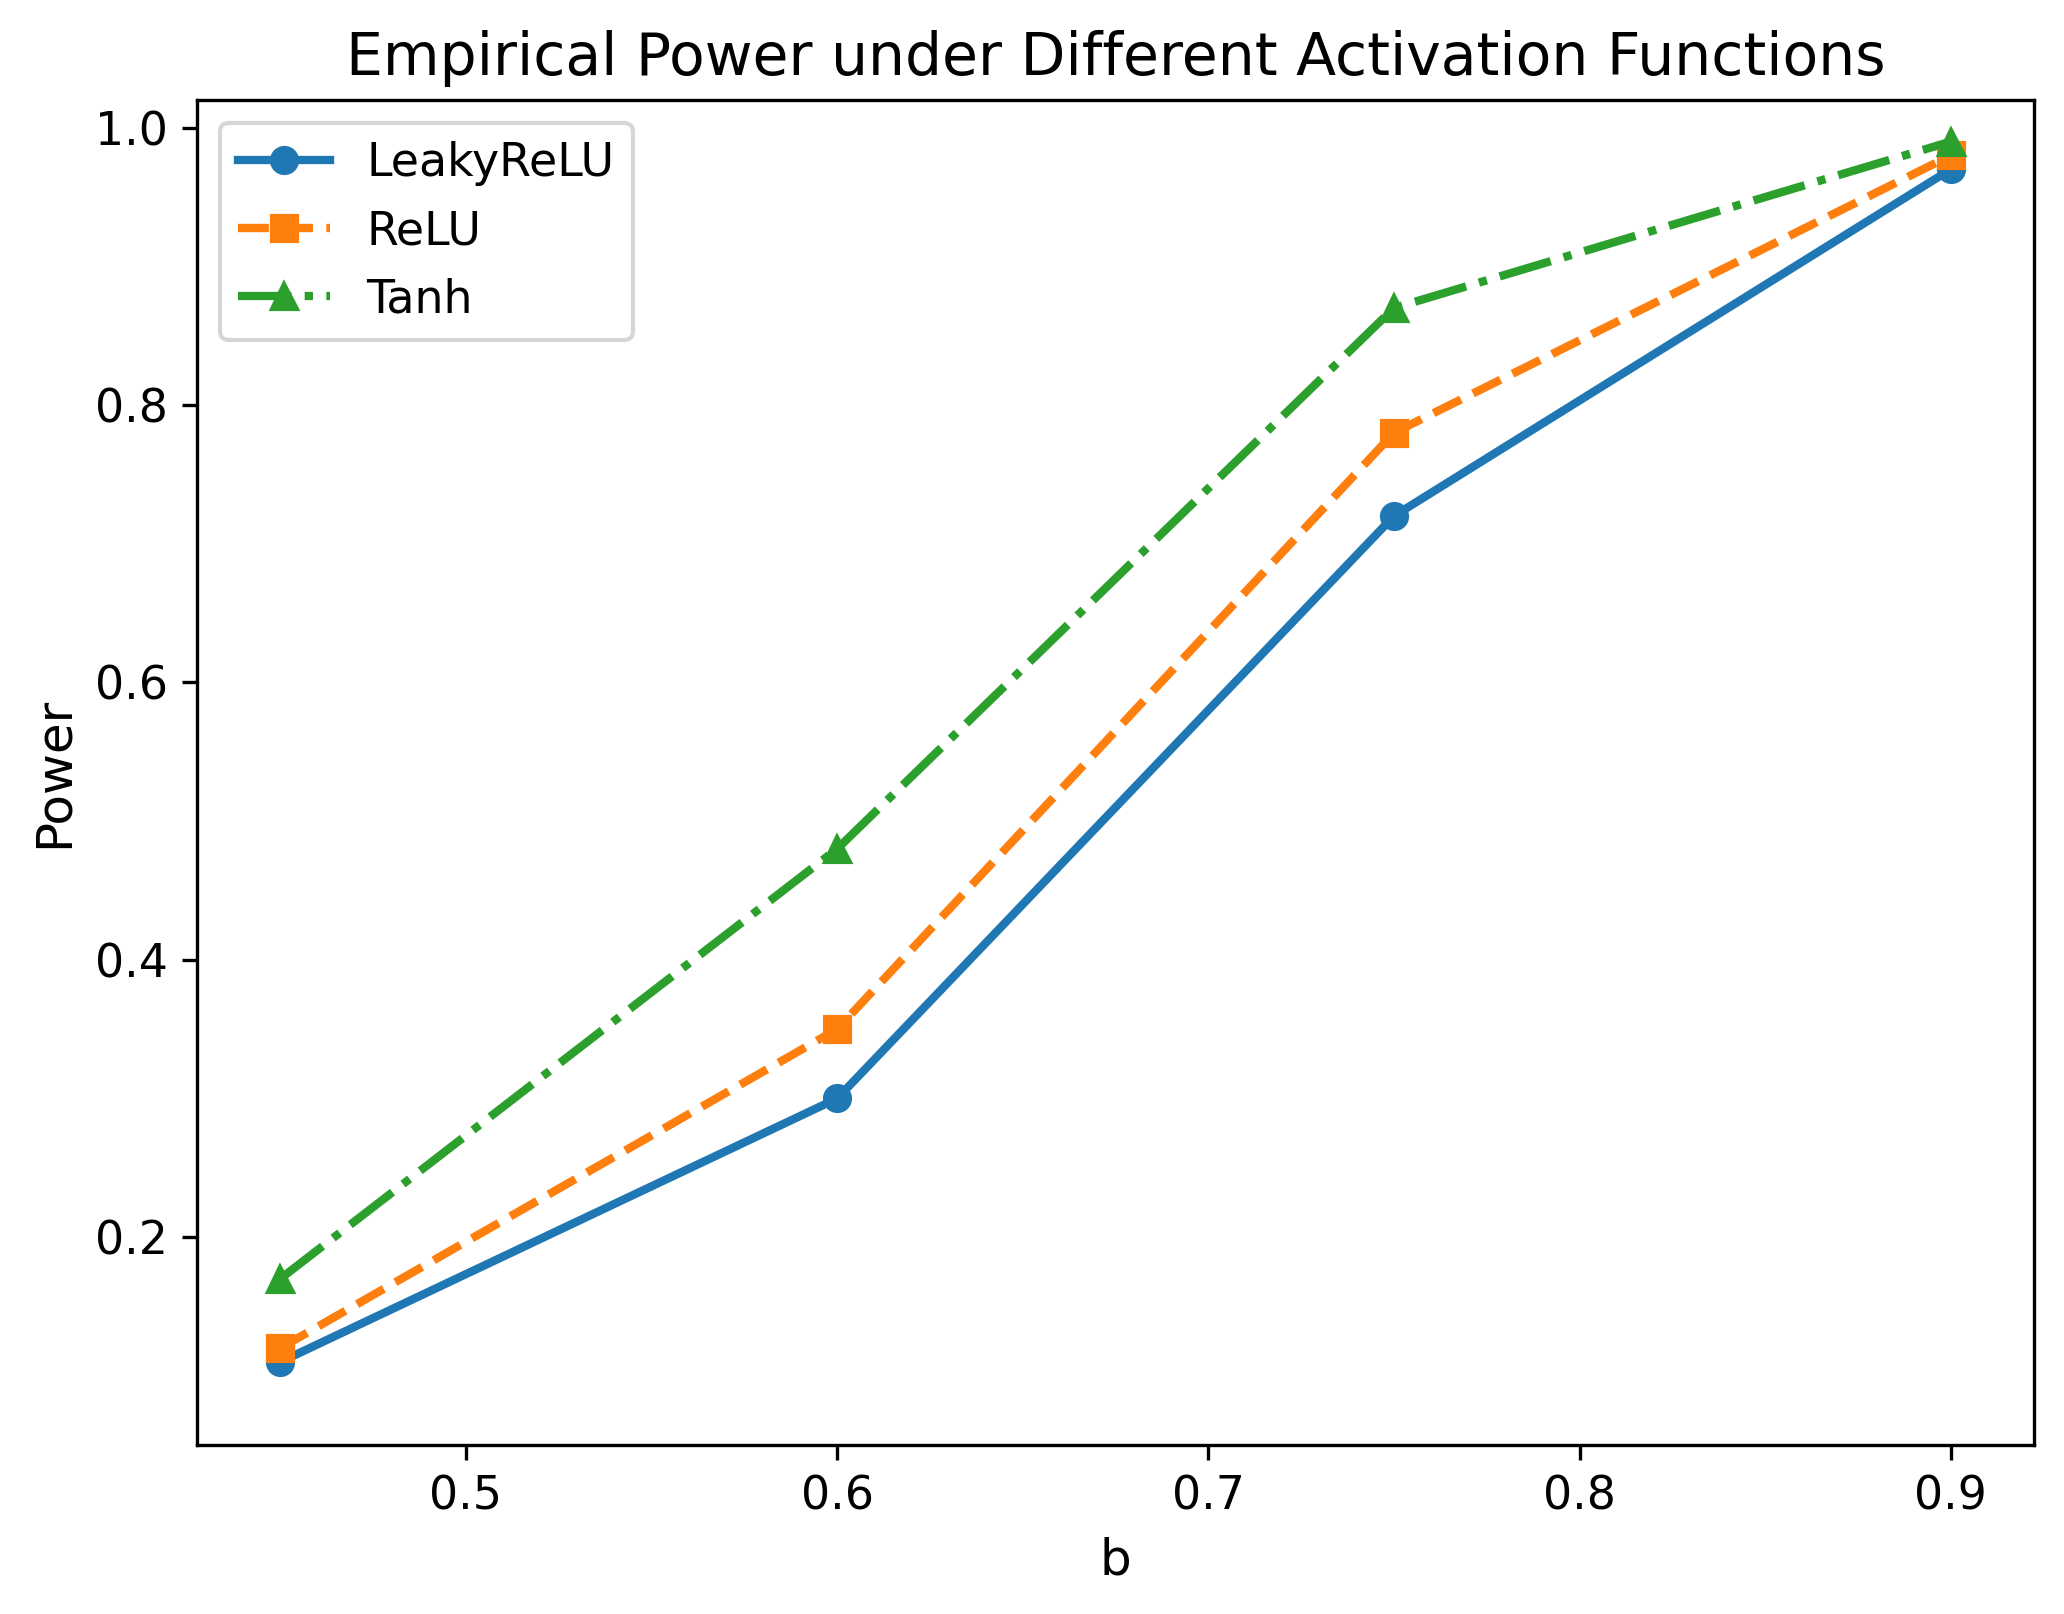
\includegraphics[width=\linewidth, alt={Empirical power of DeepBET using LeakyReLU, ReLU, and Tanh
activation functions as signal strength increases. Power increases
for all three activation functions.}]{plots/power act.png}
        \label{fig:imageB}
    \end{minipage}
    \caption{Empirical size and power of DeepBET under different activation functions.}
    \label{fig:4}
\end{figure}

\hspace{0.5cm}
Figure~\ref{fig:type 1 error} summarizes the empirical type I error rates under the null hypothesis, corresponding to $b=0$. We consider two sample sizes, $n=500$ and $n=1000$, while varying the dimension of the confounding variable over $d_Z=50,100,150,200,$ and $250$. To assess robustness with respect to the covariate distribution, $Z$ is generated from both a standard normal distribution and a Laplace distribution. The proposed DeepBET procedure is compared with the generative conditional independence test (GCIT) \cite{bellot2019conditional}, the double generative adversarial network conditional independence test (DGCIT) \cite{shi2021double}, and the classifier conditional independence test (CCIT) \cite{sen2017modelpowered}.

\hspace{0.5cm}
Overall, DeepBET maintains empirical type I error rates close to the nominal significance level across nearly all simulation settings, with only a slight inflation observed when $n=500$ and $d_Z=250$. GCIT likewise provides satisfactory type I error control throughout the experiments. In contrast, DGCIT consistently exhibits inflated type I error regardless of the simulation configuration. The performance of CCIT is less stable: its empirical size initially increases with the dimension of $Z$ before gradually decreasing as the dimensionality becomes larger.

\begin{figure}[htbp!]
    \centering
    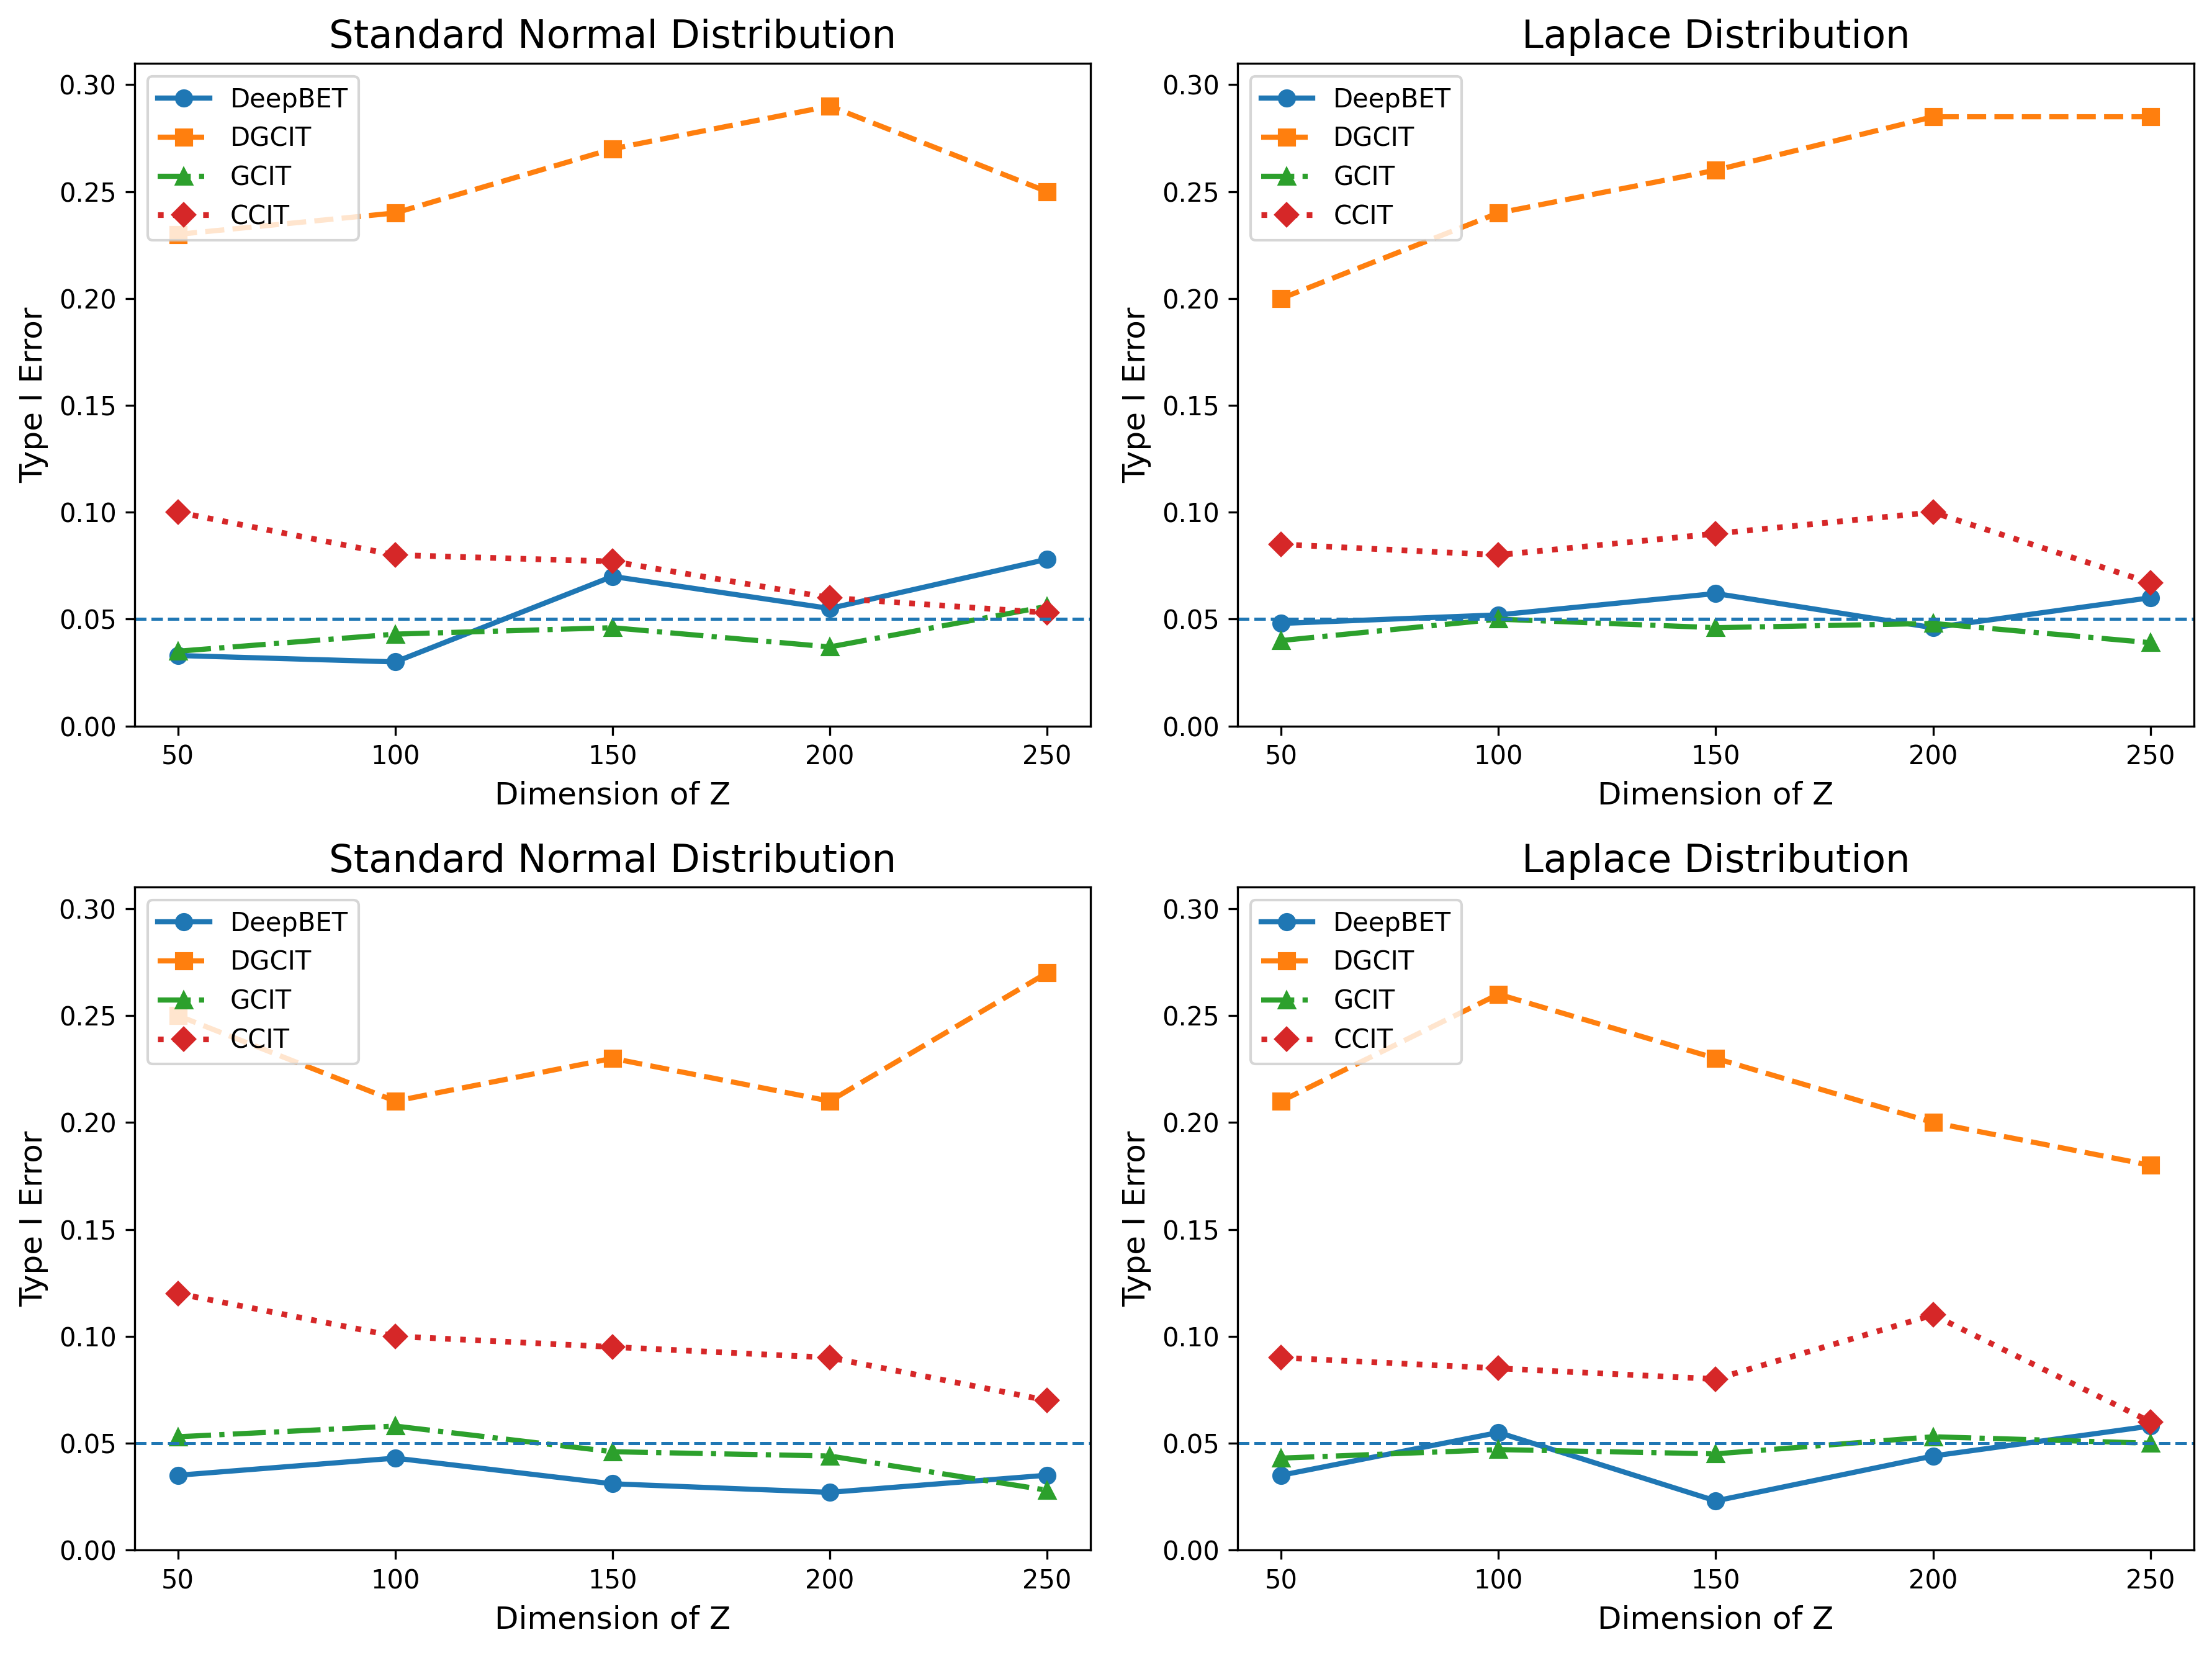
\includegraphics[width=1\linewidth, alt={Four-panel comparison of empirical Type I error for DeepBET
and competing conditional independence tests under standard normal
and Laplace error distributions across increasing dimensions of Z.}]{plots/type1error.png}
    \caption{Empirical size of different tests under $H_0$. Left panels: $Z$ follows a normal distribution. Right panels: $Z$ follows a Laplace distribution. Top panels: $n=500$. Bottom panels: $n=1000$. DeepBET maintains empirical size close to $0.05$.}
    \label{fig:type 1 error}
\end{figure}

\hspace{0.5cm}
Figure \ref{fig:power} presents the empirical power under $H_1$ with $d_Z=100$ and $b=0.45,0.6,0.75,$ and $0.9$. We again consider sample sizes $n=500$ and $n=1000$. Across all cases, DeepBET achieves higher empirical power than the competing methods, and its power approaches one as $b$ increases to $0.9$, supporting the consistency of the proposed test. By contrast, GCIT and CCIT exhibit limited power in these settings. We also compare DeepBET with the kernel-based conditional distance correlation (KCDC) test of \cite{wang2015conditional} when $n=500$ and $d_Z=100$. In this setting, the empirical size of KCDC is always equal to one, indicating that it fails to control type I error and may not be suitable for conditional independence testing with high-dimensional confounding variables.

\begin{figure}[htbp!]
    \centering
    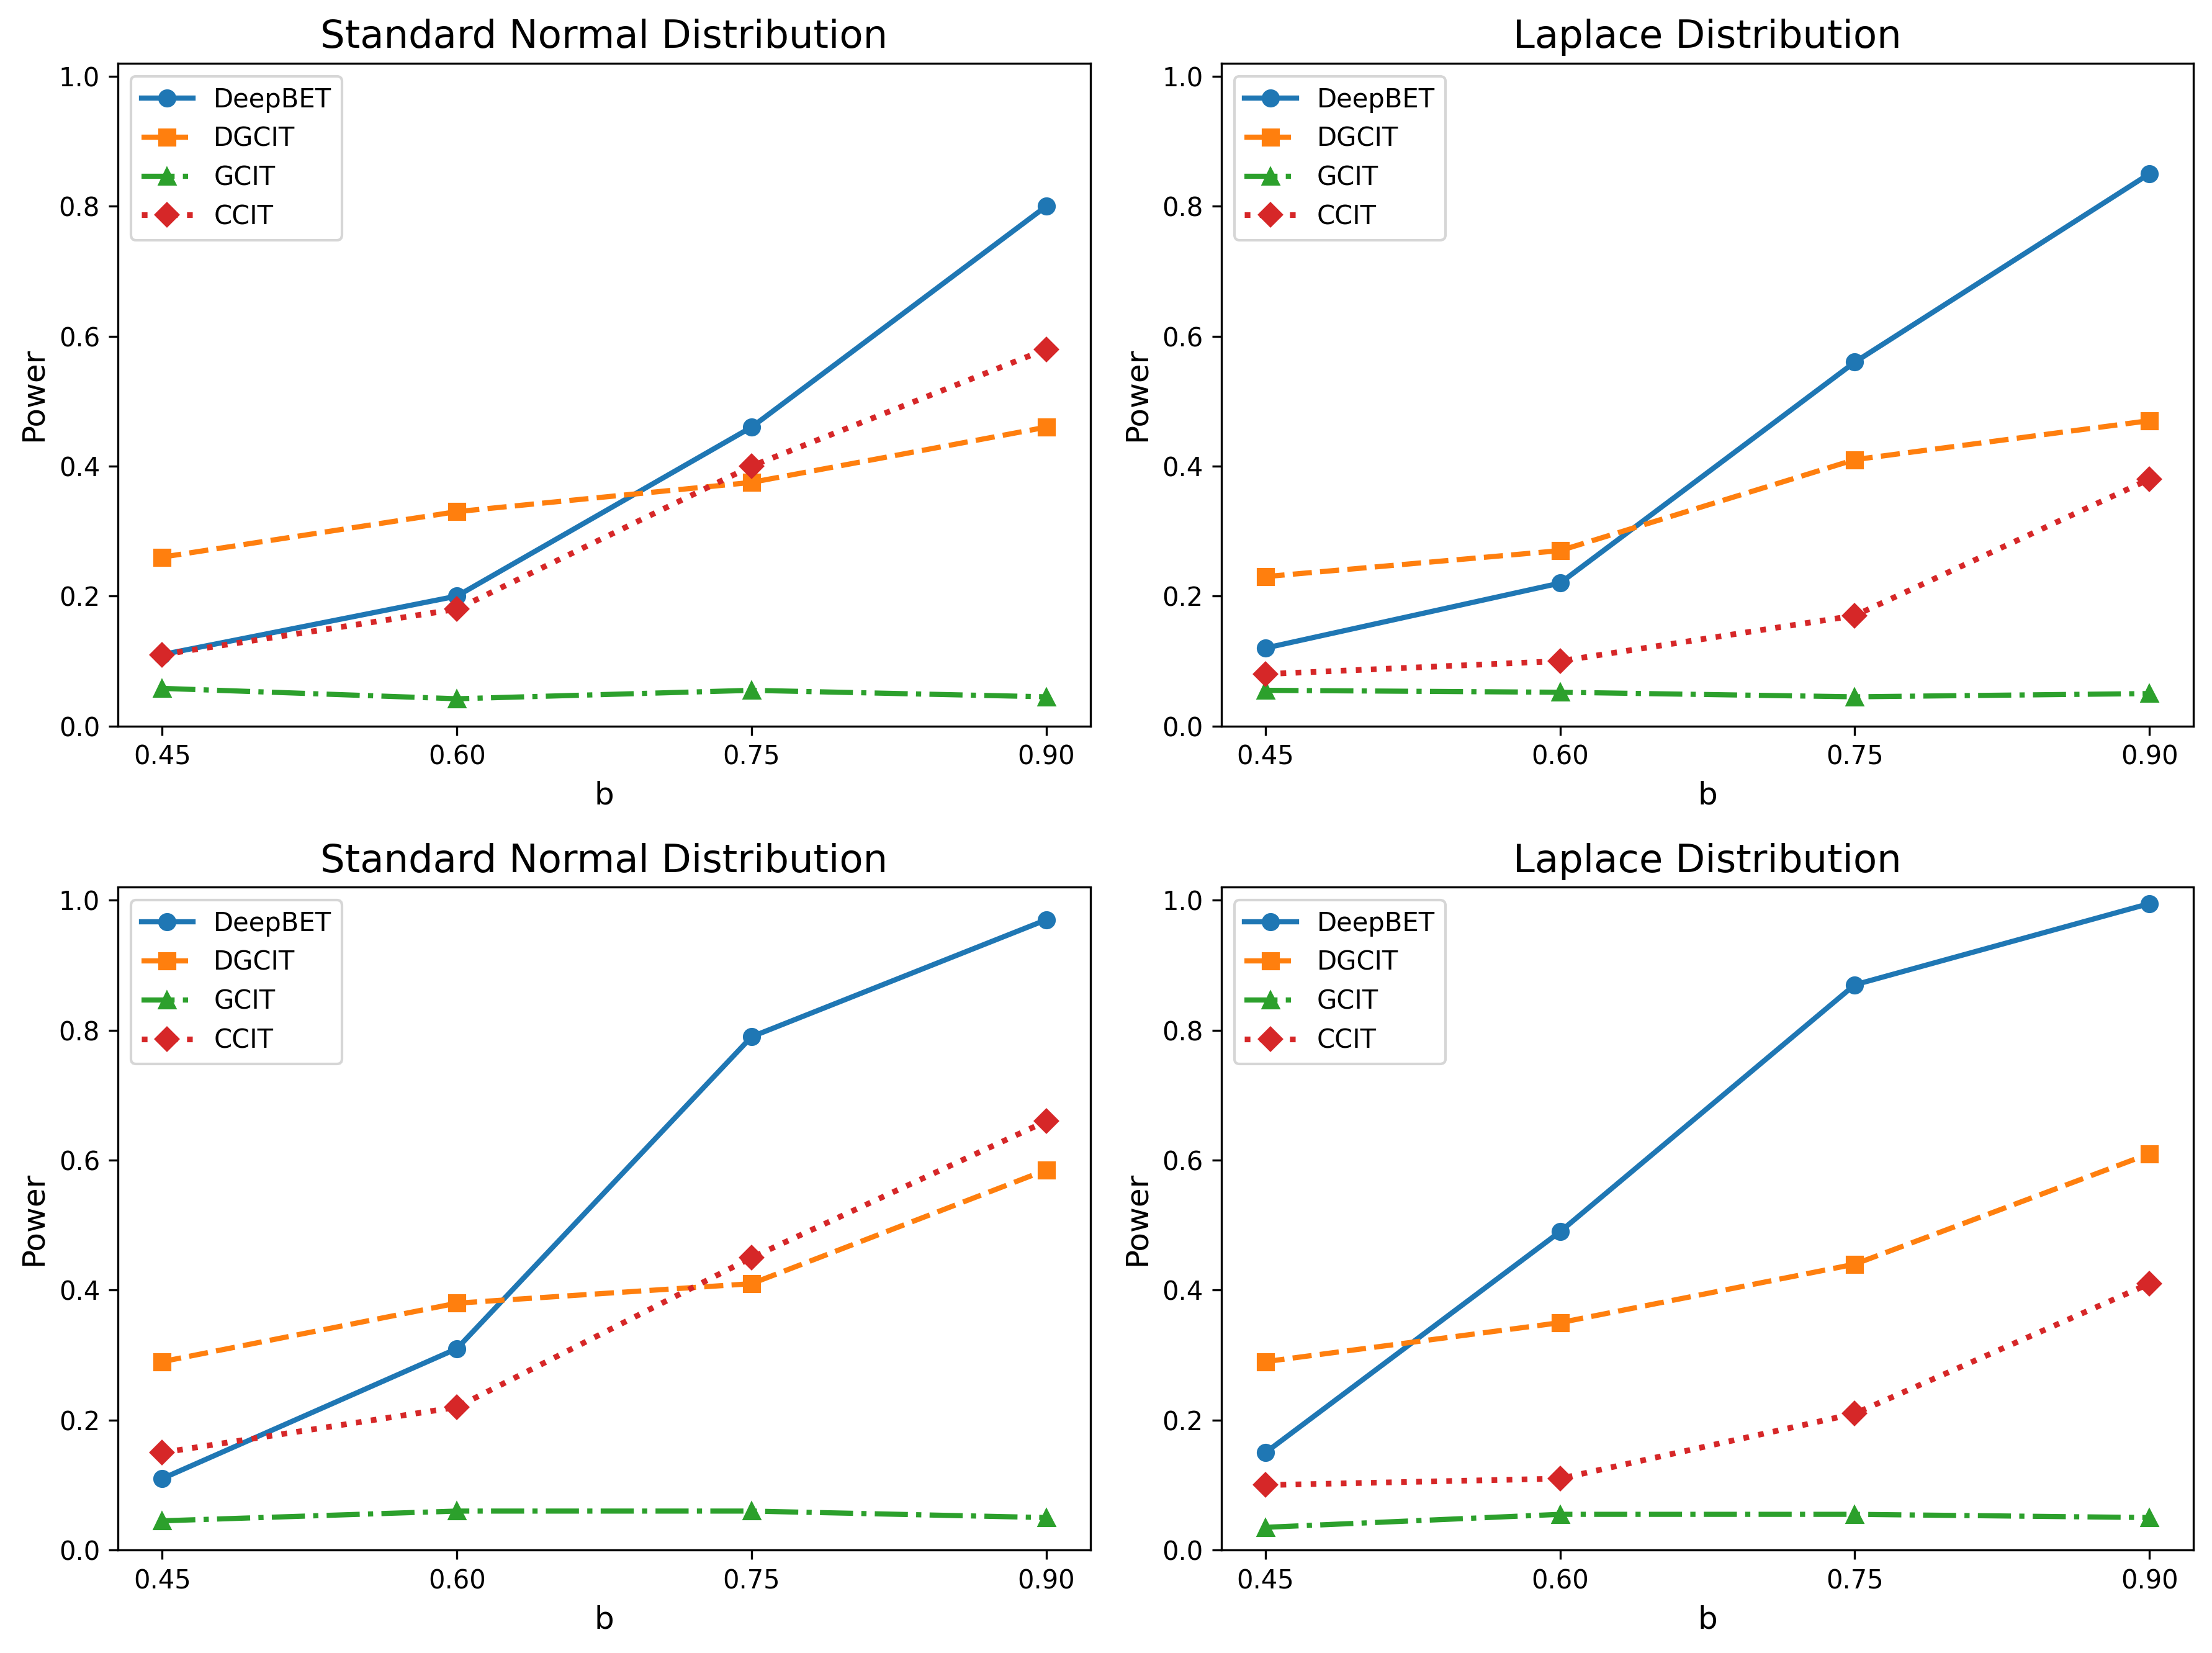
\includegraphics[width=1\linewidth, alt={Four-panel comparison of empirical power for DeepBET and
competing conditional independence tests under standard normal
and Laplace error distributions as signal strength increases.}]{plots/power.png}
    \caption{Empirical power of different tests under $H_1$. Left panels: $Z$ follows a normal distribution. Right panels: $Z$ follows a Laplace distribution. Top panels: $n=500$. Bottom panels: $n=1000$. DeepBET shows strong power across all settings.}
    \label{fig:power}
\end{figure}

\hspace{0.5cm}
Finally, we evaluate computational efficiency. All experiments are run on Google Colab using an Intel Xeon CPU with 2 vCPUs and a T4 GPU. For one simulation replication, the full DeepBET procedure takes approximately 1.5 seconds with a single split. With multiple splitting, the running time increases to about 1 minute. In comparison, CCIT takes approximately 2 minutes, GCIT takes about 20 seconds, and DGCIT takes roughly 8 minutes.



\subsubsection*{Simulation setting II}

\hspace{0.5cm}
We next consider an additional nonlinear noise model:
\begin{center}
$X= \{1+\exp(a_f^{T}Z)\}^{-1} + \epsilon_f$,\ and \ $ Y= \tanh(a_g^{T}Z+ bX)+ \nu_g,$
\end{center}
where the entries of $a_f$ and $a_g$, as well as the noise variables $\epsilon_g$ and $\nu_g$, are generated using the same setup as in Simulation Setting I. The sample size is fixed at $n=1000$, and $Z$ is generated from a standard normal distribution. The significance level is set to $\alpha=0.05$, and all reported results are based on 500 simulation replications.

\hspace{0.5cm}
We vary the dimension of $Z$ over $d_Z=50,100,150,200,$ and $250$. The proposed DeepBET method is compared with the generative conditional independence test (GCIT) of \cite{bellot2019conditional} and the DNN+GCM method based on \cite{Shah_2020}. The left panel of Figure \ref{fig:type1error1} reports empirical size under $H_0$, corresponding to $b=0$. The results suggest that DNN+GCM may exhibit inflated type I error when $d_Z=50$. The right panel of Figure \ref{fig:type1error1} compares empirical power when $d_Z=100$ and $b=0.02,0.08,$ and $0.14$, where $b$ controls the strength of the alternative. In this setting, DNN+GCM achieves the highest power, followed by DeepBET and then GCIT.

\begin{figure}[htbp!]
    \centering
    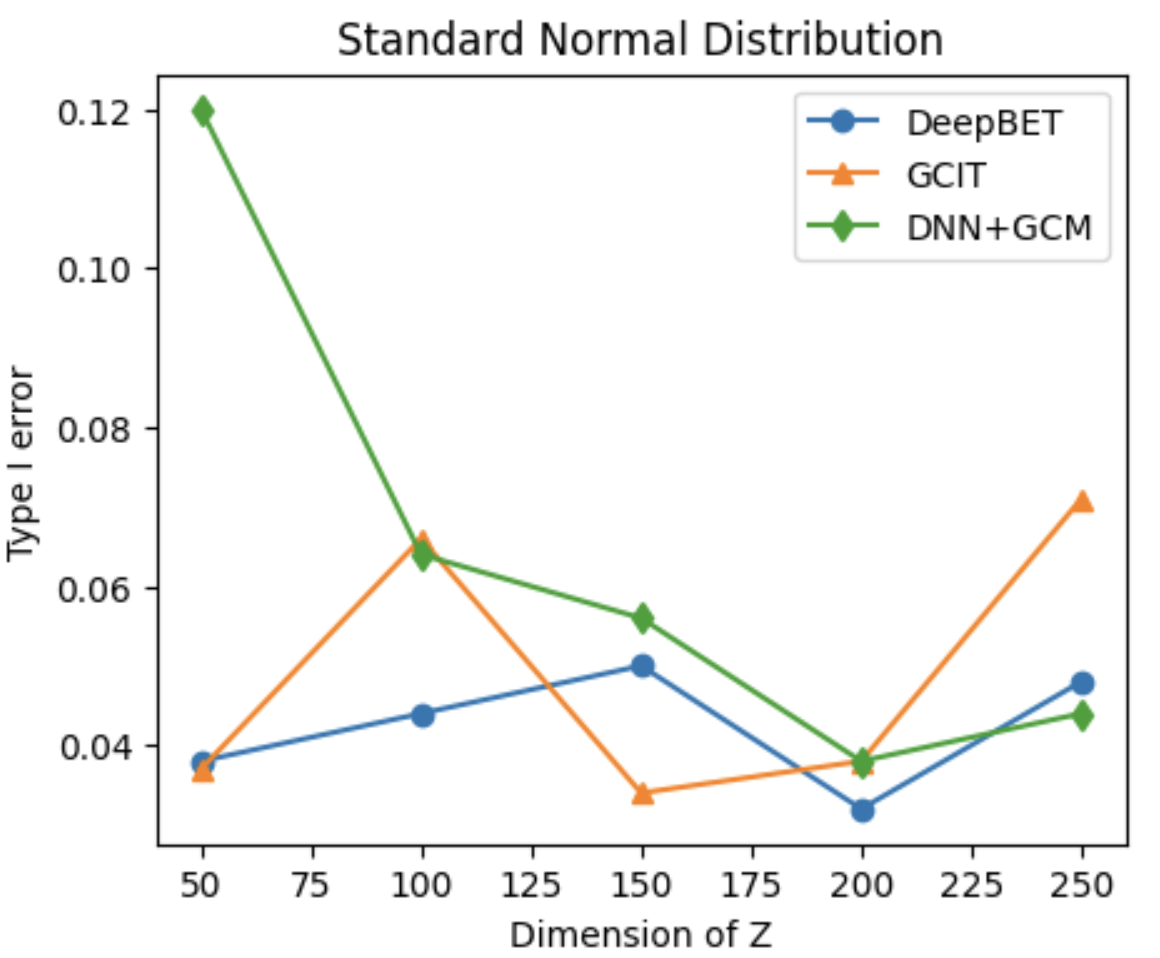
\includegraphics[width=0.45\textwidth]{plots/type1error1.png} 
    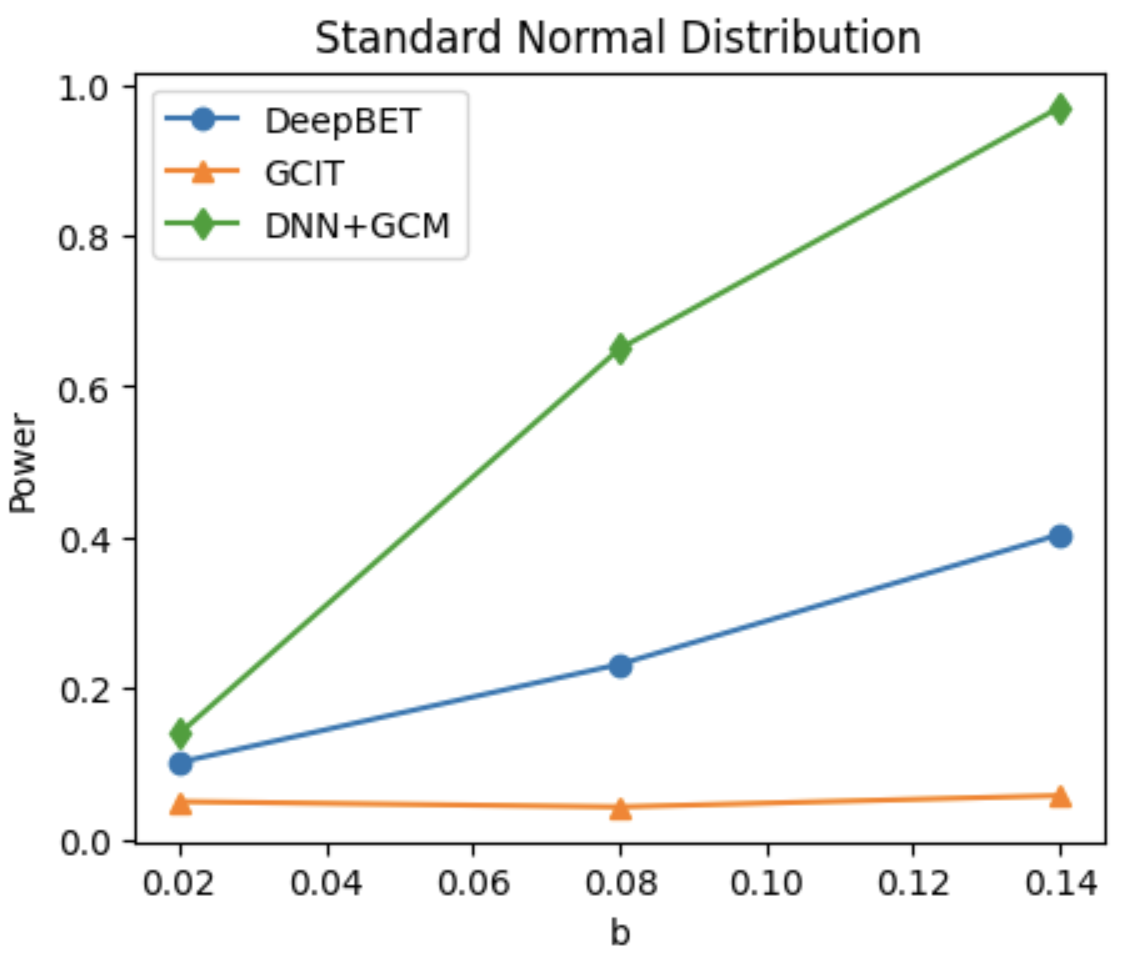
\includegraphics[width=0.45\textwidth]{plots/power1.png}
    \caption{Left panel: Empirical size of different tests under $H_0$. Right panel: Empirical power of different tests under $H_1$.}
    \label{fig:type1error1}
\end{figure}

\subsubsection*{Simulation setting III}

\hspace{0.5cm}
We further evaluate the methods under the following nonlinear noise model:
\begin{center}
$X= \sin(a_f^{T}Z) + \epsilon_f$,\ and \ $ Y= (a_g^{T}Z+ bX)^2+ \nu_g,$
\end{center}
where $a_f$, $a_g$, $\epsilon_g$, and $\nu_g$ follow the same generation scheme as in the preceding simulation settings. The sample size is set to $n=1000$, and $Z$ is generated from a standard normal distribution.

\hspace{0.5cm}
Again, we vary the dimension of $Z$ over $d_Z=50,100,150,200,$ and $250$. We compare DeepBET with DNN+GCM \cite{Shah_2020}. The left panel of Figure \ref{fig:type1error2} reports empirical size under $H_0$, where $b=0$. In this setting, DNN+GCM shows inflated type I error across all examined dimensions. The right panel of Figure \ref{fig:type1error2} reports empirical power when $d_Z=100$ and $b=0.45,0.6,0.75,$ and $0.9$. The results indicate that DNN+GCM has limited power for this nonlinear alternative.

\begin{figure}[H]
    \centering
    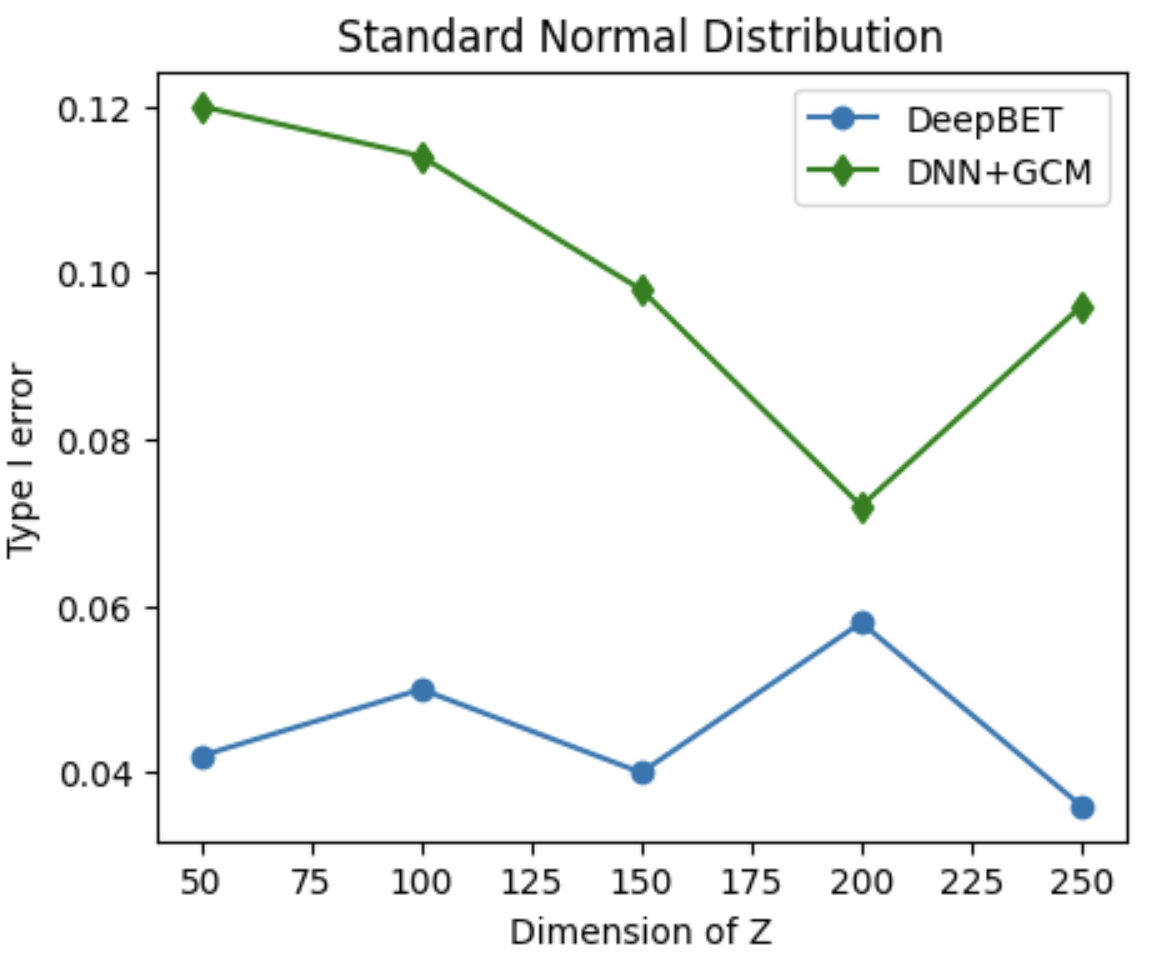
\includegraphics[width=0.45\textwidth]{plots/type1error2.png} 
    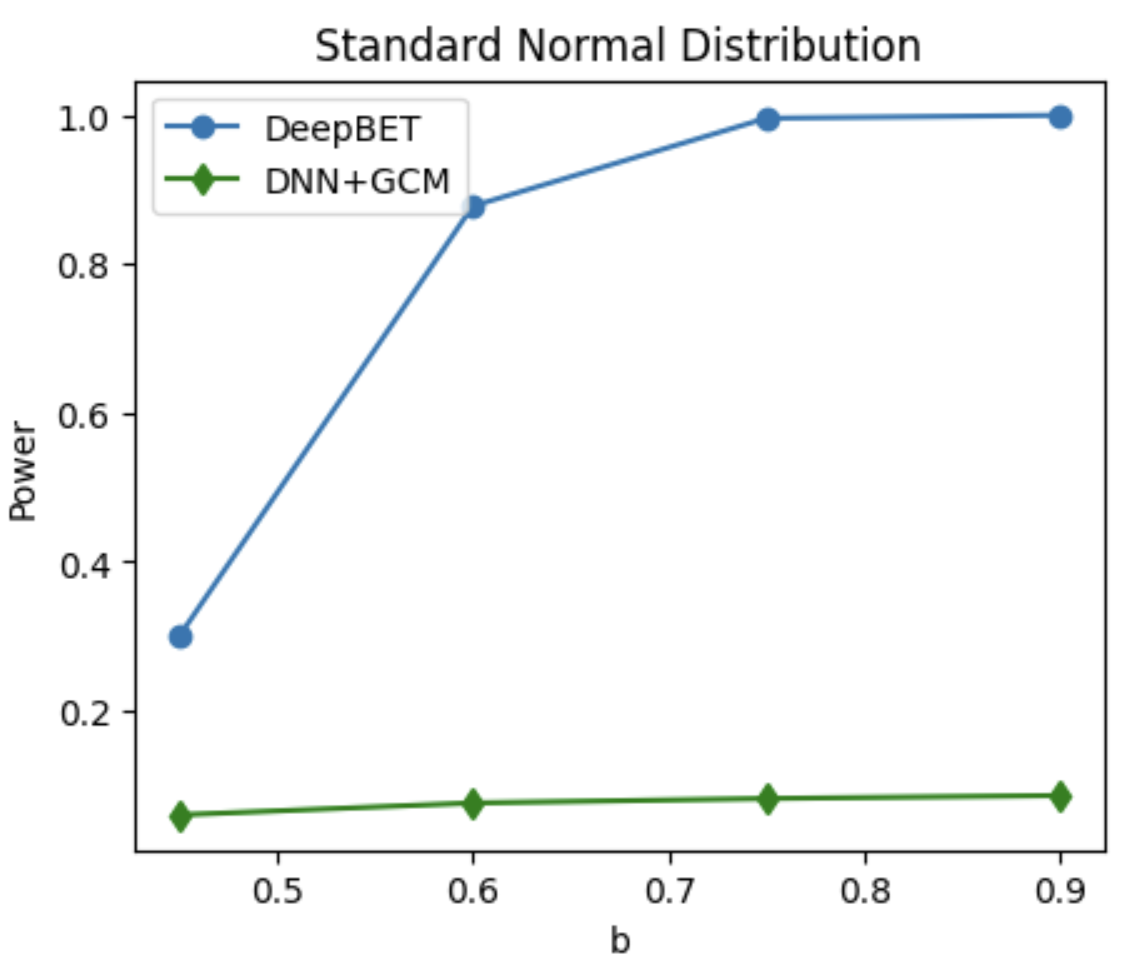
\includegraphics[width=0.45\textwidth]{plots/power2.png}
    \caption{Left panel: Empirical size of different tests under $H_0$. Right panel: Empirical power of different tests under $H_1$.}
    \label{fig:type1error2}
\end{figure}

\subsection{Analysis of Dry Eye Disease Data}

Dry eye disease (DED) refers to a heterogeneous group of ocular disorders caused by dysfunction of the ocular surface system. It can substantially affect quality of life, impose financial burden, and create broader societal costs. Symptoms range from mild discomfort to severe pain and burning, and they may interfere with sleep, visual function, and daily productivity. In the United States, DED is estimated to affect more than 16 million individuals, with a prevalence of 6.8\% among adults.

\hspace{0.5cm}
Recent clinical studies have reported thinning of the corneal epithelium among patients with DED. Figure \ref{fig:realdata} compares corneal epithelial thickness patterns between normal eyes and three different DED subtypes. Epithelial mapping is obtained using anterior segment optical coherence tomography (AS-OCT), specifically the RTVue XR OCT Avanti System (Optovue Inc., Fremont, California, USA). This imaging modality measures corneal epithelial thickness over 25 corneal regions, where darker colors indicate thinner areas.

\begin{figure}[htbp!]
    \centering
    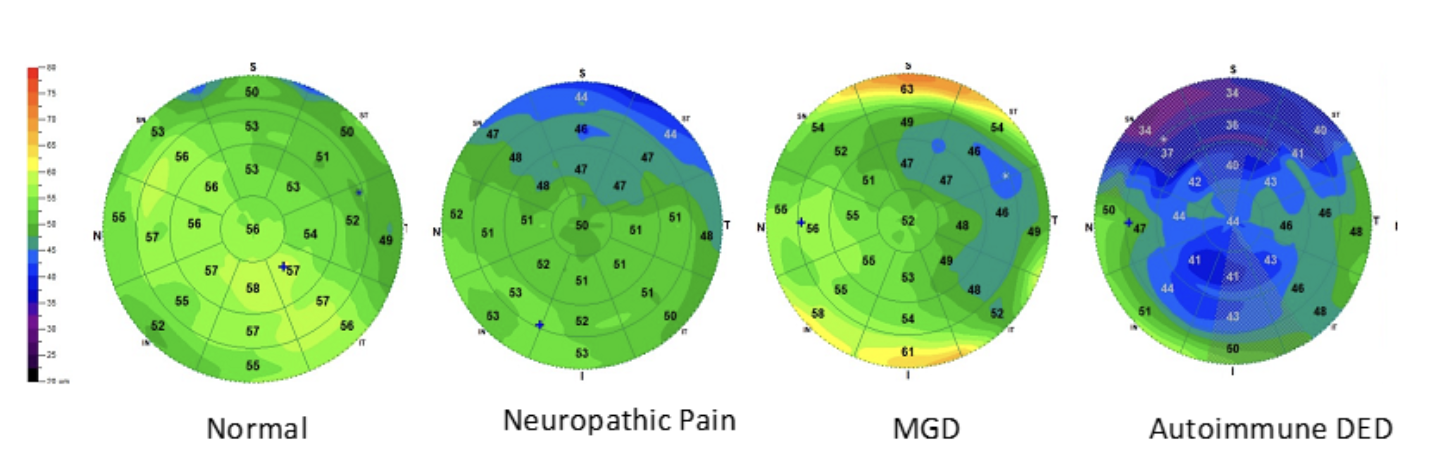
\includegraphics[width=0.9\textwidth, alt={Corneal epithelial thickness map divided into a central region
and concentric inner, middle, and outer regions with angular
subregions used in the dry eye disease analysis.}]{plots/DED map.png}
    \caption{Examples of corneal epithelial thickness maps for normal eyes and three types of dry eye disease.}
    \label{fig:realdata}
\end{figure}

\hspace{0.5cm}
The dataset contains corneal epithelial thickness measurements from 25 regions, together with Schirmer test results, for 451 eyes, including 229 right eyes and 222 left eyes. We first fit a random forest model to obtain variable importance measures. The results identify two important indicators for DED diagnosis: the Schirmer test, which measures tear production over five minutes, and the average epithelial thickness across the central 10 corneal regions. Motivated by these findings, we apply DeepBET to identify which of the 25 corneal regions exhibits the strongest association with the Schirmer test after conditioning on the remaining 24 epithelial thickness measurements.

\hspace{0.5cm}
The data are split into training and testing subsets using a $1:4$ ratio. For each analysis, the variable $X$ denotes epithelial thickness in one selected corneal region, while $Y$ denotes the Schirmer test result. The conditioning variable consists of the epithelial thickness measurements from the other 24 regions. DeepBET is first applied separately to the left-eye data to obtain region-specific $p$-values and is then applied analogously to the right-eye data. The primary goal is to determine which corneal regions are most strongly associated with tear production.

\begin{figure}[H]
    \centering
    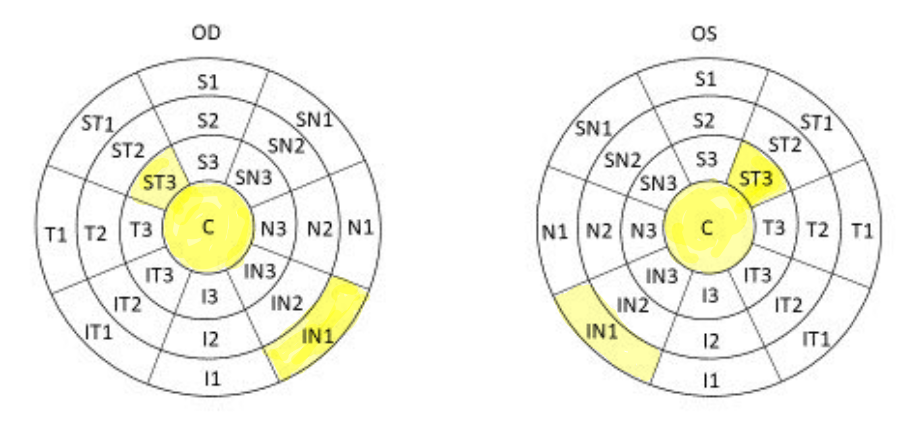
\includegraphics[width=0.85\textwidth, alt={Corneal regional dependence results from the dry eye disease
application, with highlighted regions indicating statistically
significant dependence detected by DeepBET.}]{plots/DED result.png} 
    \caption{Three highlighted epithelial thickness regions in both eyes show significant conditional dependence with the Schirmer test result.}
    \label{fig:realresults}
\end{figure}

\hspace{0.5cm}
Figure \ref{fig:realresults} shows that three epithelial thickness regions are significantly conditionally associated with tear production in both eyes after adjusting for the remaining regions. Multiplicity correction is performed using conformal $q$-values proposed by \cite{zhao2024falsediscoveryratecontrol}, with the false discovery rate controlled at 5\%.

\hspace{0.5cm}
We next examine the BET plots for selected significant regions. Figure \ref{fig:ECandC} presents the BET plots for the central region (C) of the left and right eyes, both of which yield significant test results. In these plots, $U_x$ represents epithelial thickness and $U_y$ represents tear production. Within the sigma field of binary variables, with $\mathbf{a}\neq0$ and $\mathbf{b}\neq0$, the maximal BET statistic identifies a substantially higher concentration of observations in the blue regions than in the white regions. The significant $p$-values indicate that the conditional dependence between $U_x$ and $U_y$ is driven by the interaction between the first bit of the $U_y$ residuals and the first two bits of the $U_x$ residuals.

\hspace{0.5cm}
From a clinical interpretation perspective, after conditioning on the other corneal regions, patients whose central epithelial thickness is either relatively thin, below the first quartile, or relatively thick, above the third quartile, tend to have lower tear production, below the median. This pattern is reflected by the clustering of observations in the lower-left and lower-right regions of the BET plots. By contrast, patients with central epithelial thickness between the first and third quartiles tend to show higher tear production, above the median, corresponding to the concentration of observations in the upper central region. This nonlinear dependence pattern appears consistently in both eyes. Therefore, the BET visualization provides useful heuristic interpretation in addition to formal hypothesis testing. Since many competing conditional independence tests do not directly reveal the structure of dependence after rejecting the null hypothesis, DeepBET offers an interpretable alternative.

\begin{figure}[htbp!]
    \centering
    \begin{minipage}{0.45\textwidth}
        \centering
        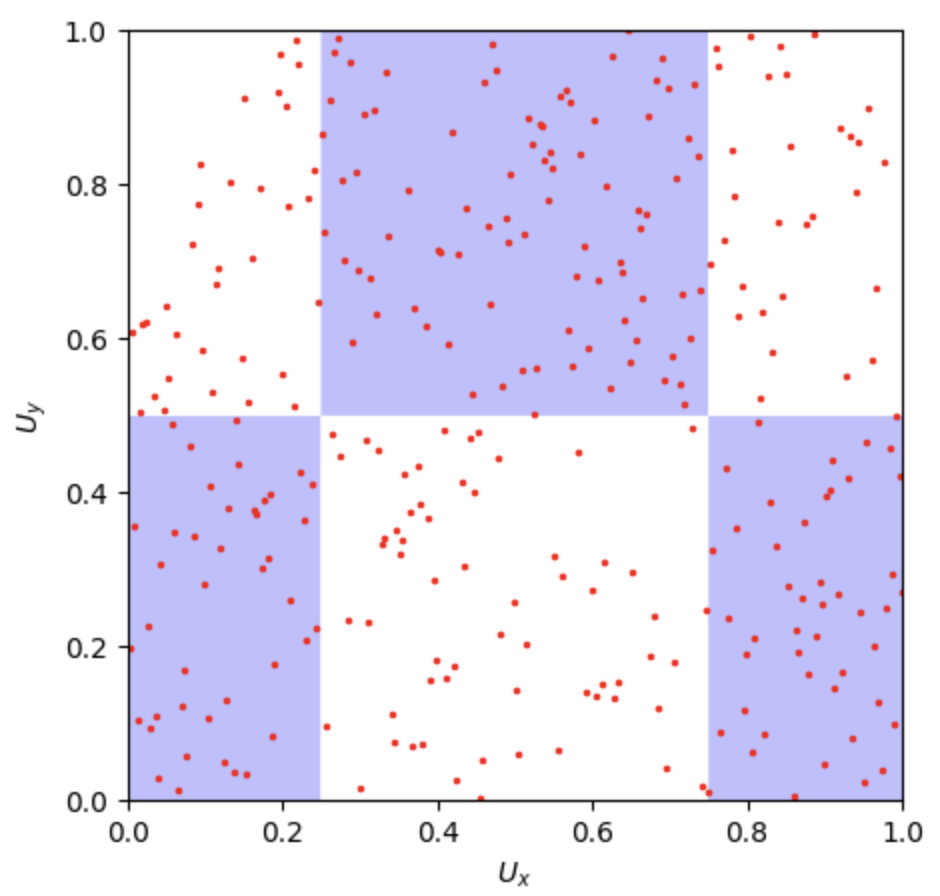
\includegraphics[width=\linewidth,height=6.8cm, alt={Binary expansion dependence pattern illustrating the C-type
interaction detected between the transformed variables.}]{plots/C.png}
        \label{fig:imageC}
    \end{minipage} \hfill
    \begin{minipage}{0.45\textwidth}
        \centering
        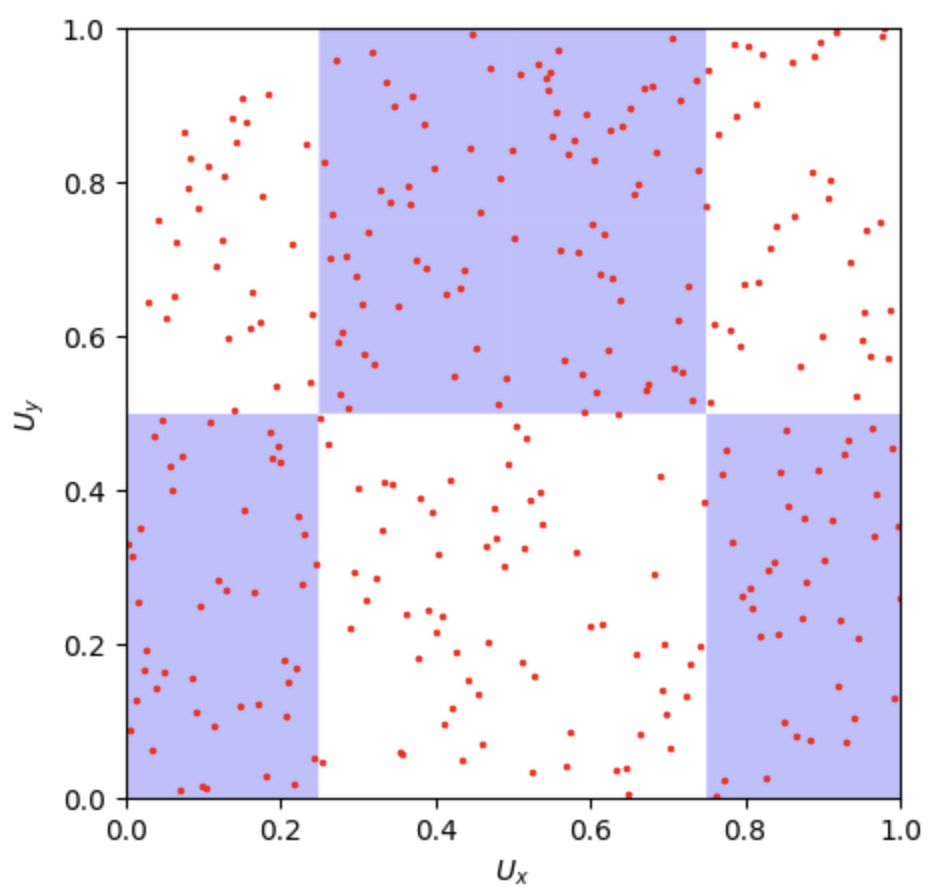
\includegraphics[width=\linewidth,height=6.8cm, alt={Binary expansion dependence pattern illustrating the EC-type
interaction detected between the transformed variables.}]{plots/EC.png}
        \label{fig:imageES}
    \end{minipage}
    \caption{Left: BET visualization for the central (C) region of the left eye. Right: BET visualization for the corresponding central region of the right eye. Both conditional independence tests are statistically significant, and each plot exhibits a noticeably greater concentration of observations in the blue regions than in the white regions. This consistent pattern indicates a similar nonlinear association between central epithelial thickness and tear production in both eyes after adjusting for the remaining corneal regions.}
    \label{fig:ECandC}
\end{figure}



\section{Discussion}
\label{discussion}

This chapter introduced \textbf{DeepBET}, a new procedure for testing conditional independence in the presence of high-dimensional confounding variables. The proposed framework integrates three complementary components: deep neural networks (DNNs) for estimating conditional mean functions, Binary Expansion Testing (BET) for distribution-free dependence testing, and a multiple-splitting strategy for improving finite-sample performance. Together, these components yield a conditional independence test that is both computationally scalable and theoretically well justified.

The proposed DeepBET procedure possesses several desirable properties. Theoretically, it is uniformly consistent against general alternatives and achieves a root-$n$ convergence rate despite relying on nonparametric estimation in high-dimensional settings. Empirically, extensive simulation studies demonstrate that DeepBET effectively controls the type I error, achieves competitive or superior power relative to existing methods, remains computationally efficient, and is relatively insensitive to the choice of DNN tuning parameters. In addition, the BET representation provides interpretable information about the underlying dependence structure, a feature that is often unavailable in competing conditional independence tests.

The theoretical results presented in this chapter complement the rapidly growing literature on statistical estimation and inference using modern machine learning techniques. In particular, they are closely related to recent developments in semiparametric inference involving low-dimensional target parameters and high-dimensional nuisance functions estimated by machine learning methods (e.g., \cite{Chernozhukov2018,Farrell2021}). Compared with the substantial literature on machine-learning-based estimation and inference, however, relatively little work has investigated the use of deep neural networks for conditional independence testing. The proposed DeepBET framework provides one step in this direction by combining flexible DNN estimation with a distribution-free and interpretable testing procedure.





\section{Technical Proofs}
\label{tech_proof}

This section presents the technical assumptions and preliminary results required for establishing the asymptotic properties of the proposed DeepBET procedure. We begin by introducing the smoothness conditions imposed on the regression functions $h(\cdot)$ and $g(\cdot)$, together with the hierarchical neural network architecture used to approximate these functions.

\begin{definition}
A function $m:\mathbb{R}^d\rightarrow\mathbb{R}$ is said to be $(p,C)$-smooth if its partial derivatives of order $q$ exist and satisfy
\[
\left|
\frac{\partial^q m(z)}
{\partial z_1^{\alpha_1}\cdots\partial z_d^{\alpha_d}}
-
\frac{\partial^q m(x)}
{\partial z_1^{\alpha_1}\cdots\partial z_d^{\alpha_d}}
\right|
\le
C\|z-x\|^s,
\]
for every $x,z\in\mathbb{R}^d$, where
$\sum_{j=1}^d\alpha_j=q$ and $p=q+s$.

A function $m(z)$ is called a generalized hierarchical interaction model of order $d_*$ and level $0$ if there exist vectors
$a_1,\ldots,a_{d_*}\in\mathbb{R}^d$
and a mapping
$f:\mathbb{R}^{d_*}\rightarrow\mathbb{R}$
such that
\[
m(z)=f(a_1^Tz,\ldots,a_{d_*}^Tz),
\qquad
\forall\,z\in\mathbb{R}^d.
\]

Then, $m(z)$ is a generalized hierarchical interaction model of order $d_*$ and level $l+1$ if there exist $K$, $\theta_k(\cdot)$, and $f_{1,k},\cdots,f_{d_*,k}$ such that
\[
m(z)
=
\sum_{k=1}^K
\theta_k
\{f_{1,k}(z),\cdots,f_{d_*,k}(z)\},
\]
where each
$f_{1,k},\cdots,f_{d_*,k}$
is itself a generalized hierarchical interaction model of order $d_*$ and level $l$. If every function
$f(\cdot)$,
$\theta_k(\cdot)$,
and
$f_{1,k},\cdots,f_{d_*,k}$
is $(p,C)$-smooth, then
$m(z)$
is called a $(p,C)$-smooth generalized hierarchical interaction model.
\end{definition}

\begin{definition}
\label{hnn}
A hierarchical neural network $\mathcal{H}^{(l)}$ is defined recursively given by the following:
\begin{align*}
\mathcal{H}^{(l)}
=
\{
h:
h(z)
=
\sum_{k=1}^K
\theta_k(f_{1,k}(z),\cdots,f_{d_*,k}(z))
\;
\mbox{for some}
\;
g_k\in\mathcal{F}_{M^*,d_*,d,\alpha}^{NN}
\;
\mbox{and}
\;
f_{j,k}\in\mathcal{H}^{(l-1)}
\}.
\end{align*}
and
$\mathcal{H}^{(0)}=\mathcal{F}_{M^*,d_*,d,\alpha}^{NN}$.

Here
$\mathcal{F}_{M^*,d_*,d,\alpha}^{NN}$
denotes the collection of neural networks of the form
$$
f(z)
=
\sum_{j=1}^{M^*}
\mu_i
\sigma
\Big(
\sum_{j=1}^{4d_*}
\lambda_{i,j}
\sigma
\Big(
\sum_{v=1}^d
\theta_{i,j,\nu}z_v+\theta_{i,j,0}
\Big)
+\lambda_{i,0}
\Big)
+\mu_0,
$$
for some
$|\mu_i|\leq\alpha$,
$|\lambda_{i,j}|\leq\alpha$,
$|\theta_{i,j,\nu}|\leq\alpha$,
and activation function
$\sigma(\cdot)$.
\end{definition}

To estimate the unknown regression function $h(\cdot)$, we consider the least-squares estimator
\begin{align}
\label{hestimator}
\hat{h}
=
\arg\min_{h\in\mathcal{H}^{(l)}}
\sum_{i=1}^n
\left(X_i-h(Z_i)\right)^2,
\end{align}
where the function class $\mathcal{H}^{(l)}$ is defined in Definition \ref{hnn}. In practice, the optimization problem in (\ref{hestimator}) is solved numerically using gradient-based optimization methods, such as stochastic gradient descent and its variants. Since these algorithms do not necessarily attain the global optimum, the convergence guarantee stated in Lemma \ref{lemma1} should be interpreted under the assumption that the optimization procedure achieves the desired estimator. Throughout the theoretical development, we impose the following regularity conditions.

\begin{itemize}

\item[(C1)]
The covariate vector $Z\in\mathbb{R}^d$ has bounded support. The regression functions
$h(z)$
and
$g(z)$
are assumed to satisfy the $(p,C)$-smooth generalized hierarchical interaction model of order $d_*$ and finite level $l$, where $p=q+s$ for some nonnegative integer $q$ and $s\in(0,1]$.

\item[(C2)]
The observations
$(X_1,Y_1,Z_1),\ldots,(X_n,Y_n,Z_n)$
are independent and identically distributed. Furthermore,
$E\{\exp(c_1X^2)\}<\infty$
and
$E\{\exp(c_2Y^2)\}<\infty$
for some positive constants
$c_1$
and
$c_2$.

\end{itemize}

The following approximation result, established by \cite{Bauer2019}, provides the convergence rate of the DNN estimator under the above assumptions.

\begin{lemma}
\label{lemma1}
Suppose that conditions (C1) and (C2) are satisfied. Furthermore, assume that all partial derivatives of $\theta_k$ and $f_{j,k}$ up to order $q$ are bounded, and that $\theta_k$ is Lipschitz continuous. Let
\[
M^*\asymp c n^{d_*/(2p+d_*)}, \qquad
\alpha\asymp n^c,
\]
for a sufficiently large constant $c$, and assume that the activation function $\sigma(\cdot)$ is $N$-admissible. Then the estimator obtained by solving the optimization problem in (\ref{hestimator}) satisfies
\[
E\|\hat{h}-h\|_2^2
\leq
c n^{-2p/(2p+d_*)}\log^3(n),
\]
for sufficiently large $n$.
\end{lemma}

The following lemma extends the product-difference inequality of \cite{Bickel_2008} from two factors to products involving an arbitrary number of terms ($l\ge2$).

\begin{lemma}
\label{lemma2}
Let $I_a=\sum_{1\leq v_1<\cdots<v_a\leq l}^l\prod_{j=1}^a |C^{(v_j)}-\tilde{C}^{(v_j)}| 
\prod_{j\neq v_1,\cdots, v_a}^a |\tilde{C}^{(j)}|$. Then, the following inequality holds: 
\begin{align*}
\left|\prod_{j=1}^l C^{(j)}-\prod_{j=1}^l \tilde{C}^{(j)} \right| &\le \sum_{a=1}^l I_a. 
\end{align*}
\end{lemma}


\textbf{Proof of Lemma \ref{lemma2}}: Note that we can write 
\begin{align*}
\prod_{j=1}^l C^{(j)}&= \prod_{j=1}^l \{(C^{(j)}-\tilde{C}^{(j)}) + \tilde{C}^{(j)}\}\\
&= \prod_{j=1}^l\tilde{C}^{(j)} +\sum_{a=1}^l \sum_{1\leq v_1<\cdots<v_a\leq l}^l\prod_{j=1}^a (C^{(v_j)}-\tilde{C}^{(v_j)}) 
\prod_{j\neq v_1,\cdots, v_a}^a \tilde{C}^{(j)}.
\end{align*}
It then follows that
\begin{align*}
\left|\prod_{j=1}^l C^{(j)}-\prod_{j=1}^l \tilde{C}^{(j)} \right|\leq \sum_{a=1}^l \sum_{1\leq v_1<\cdots<v_a\leq l}^l\prod_{j=1}^a |C^{(v_j)}-\tilde{C}^{(v_j)}| 
\prod_{j\neq v_1,\cdots, v_a}^a |\tilde{C}^{(j)}|.
\end{align*}
This completes the proof of Lemma 2.



\textbf{Proof of Theorem~1.}
Since the sample size of the testing set, $n_{\mathcal{D}_2}$, is proportional to the full sample size $n$, we use $n$ in place of $n_{\mathcal{D}_2}$ throughout the proof to simplify the notation. By Theorem 4.2 of \cite{zhang2019bet},
\[
\frac{S_{(\mathbf{ab}),n}+n}{4}
\sim
\mathrm{Hypergeometric}(n,n/2,n/2).
\]
Therefore, to establish
\[
\frac{\hat{S}_{(\mathbf{ab}),n}+n}{4}
\sim
\mathrm{Hypergeometric}(n,n/2,n/2),
\]
it is sufficient to verify that
\[
|\hat{S}_{(\mathbf{ab}),n}-S_{(\mathbf{ab}),n}|
=
o_p\!\left\{S_{(\mathbf{ab}),n}\right\}.
\]

To this end, we first decompose the difference between the estimated statistic and its population counterpart as
\begin{align*}
|\hat{S}_{(\mathbf{ab}),n}-S_{(\mathbf{ab}),n}|
&=
|\hat{S}_{(\mathbf{ab}),n}-\hat{S}_{h_{(\mathbf{ab}),n}}
+\hat{S}_{h_{(\mathbf{ab}),n}}
-S_{h_{(\mathbf{ab}),n}}
+S_{h_{(\mathbf{ab}),n}}
-S_{(\mathbf{ab}),n}|\\
&\le
|\hat{S}_{(\mathbf{ab}),n}-\hat{S}_{h_{(\mathbf{ab}),n}}|
+
|\hat{S}_{h_{(\mathbf{ab}),n}}
-S_{h_{(\mathbf{ab}),n}}|
+
|S_{h_{(\mathbf{ab}),n}}
-S_{(\mathbf{ab}),n}|,
\end{align*}
where $S_{h_{(\mathbf{ab}),n}}$ denotes a smoothed version of
$S_{(\mathbf{ab}),n}$, which will be introduced later.

The remainder of the proof proceeds in three steps. We establish that each term on the right-hand side is asymptotically negligible relative to $S_{(\mathbf{ab}),n}$. Consequently,
\[
|\hat{S}_{(\mathbf{ab}),n}-S_{(\mathbf{ab}),n}|
=
o_p\!\left\{S_{(\mathbf{ab}),n}\right\},
\]
which proves the desired result.

\medskip
\textbf{Step 1.}
Let $\hat{\epsilon}_i$ and $\hat{\nu}_i$ denote the residuals obtained from the DNN estimators. Let $F$ and $G$ be the corresponding cumulative distribution functions of $\hat{\epsilon}_i$ and $\hat{\nu}_i$, respectively. Define the probability integral transforms
\[
\hat{U}_i=F(\hat{\epsilon}_i),
\qquad
\hat{V}_i=G(\hat{\nu}_i).
\]
The binary expansion coefficients used by DeepBET are then constructed from the transformed residuals. Specifically,
Let us construct a smoothed version of $\hat{A}_{{h}_i}^{(k)}$ so that it transitions smoothly 
from -1 to +1. That is
\begin{equation} 
    \hat{A}_{{h}_i}^{(k)} = \begin{cases} 
     
      -1 & if\quad   \frac{2k-2}{2^{d_1}} < \hat{U}_{i} < \frac{2k-1}{2^{d_1}}-h \\
      -1 + 2( \,\int_{{\frac{2k-1}{2^{d_1}}}-h}^{\substack{\hat{U}_i}} \psi(\frac{t-(\frac{2k-1}{2^{d_1}})}{h}) dt/ \int_{{\frac{2k-1}{2^{d_1}}}-h}^{\substack{\frac{2k-1}{2^{d_1} } +h}}  \psi(\frac{t-(\frac{2k-1}{2^{d_1}})}{h}) dt ) \,  & if\quad \frac{2k-1}{2^{d_1}}-h \leq \hat{U}_{i} \leq \frac{2k-1}{2^{d_1}} +h \\
      +1 & if \quad \frac{2k-1}{2^{d_1}} + h < \hat{U}_{i}< \frac{2k}{2^{d_1}}
   \end{cases}
\end{equation}
where $\psi(x)$ is a bump function which is infinitely differentiable defined by
\begin{equation} 
    \psi(x) = \begin{cases} 
       e^{-{1}/{(1-x^2)}}& for -1<x<1 \\
       0 & otherwise.
   \end{cases}
\end{equation}

The difference between $\hat{A}_i^{(k)}$ and $\hat{A}_{h_i}^{(k)}$ occurs only in the interval $[\frac{2k-1}{2^{d_1}}-h, \frac{2k-1}{2^{d_1}} +h]$. Outside of this region, both functions are identical.
Define the event where $\hat{A}_i^{(k)}$ and $\hat{A}_{h_i}^{(k)}$ differ:
\[
\mathcal{E}_A := \left\{ \hat{U}_i \in \left( \frac{2k-1}{2^{d_1}} - h, \frac{2k-1}{2^{d_1}} + h \right) \right\}.
\]
Then, for any $u>0$,
$$
P(|\hat{A}_i^{(k)}-\hat{A}_{{h}_i}^{(k)}|>u)
\leq \mathbb{P} \left( \hat{A}_i^{(k)} \neq \hat{A}_{{h}_i}^{(k)} \right) = \mathbb{P} \left( \mathcal{E}_A \right) = \int_{\frac{2k-1}{2^{d_1}} - h}^{\frac{2k-1}{2^{d_1}} + h} f_{\hat{U}_i}(u) du,
$$
where $f_{\hat{U_i}}(u)$ denote the probability density function of $\hat{U_i}$.

When $h$ is small and the density $f_{\hat{U_i}}(u)$ is bounded, the above integration can be approximated by the following:
   \[
   \mathbb{P}\left( \mathcal{E}_A \right) \approx f_{\hat{U}_i}\left( \frac{2k-1}{2^{d_1}} \right) \cdot \left( \frac{2k-1}{2^{d_1}} + h - \left( \frac{2k-1}{2^{d_1}} - h \right) \right) = 2h \cdot f_{\hat{U}_i}\left( \frac{2k-1}{2^{d_1}} \right)= \mathcal{O}(h).
   \]


Thus, we have:

\[
|\hat{A}_i^{(k)} - \hat{A}_{{h}_i}^{(k)}| = \mathcal{O}_p(h).
\]

Similarly, we can also construct a smoothed version of $\hat{B}_i^{(k)}$ using $\hat{B}_{{h}_i}^{(k)}$. 
Using the same approach, we can bound the difference between $\hat{B}_{i}^{(k)}$ and $\hat{B}_{{h}_i}^{(k)}$ by
\[
|\hat{B}_i^{(k)} - \hat{B}_{{h}_i}^{(k)}| = \mathcal{O}_p(h).
\]

Now, we will bound the difference 
$\hat{S}_{{(\mathbf{ab}),n_i}}$ and $\hat{S}_{h_{(\mathbf{ab}),n_i}}$. Recall that
$$
\hat{S}_{(\mathbf{ab}),n_i}=\prod_{k=1}^{d_1} \{\hat{A}_{i}^{(k)}\}^{a_k} \prod_{k=1}^{d_2} \{\hat{B}_{i}^{(k)}\}^{b_k},
;\mbox{and}\; \hat{S}_{h_{(\mathbf{ab}),n_i}}=\prod_{k=1}^{d_1} \{\hat{A}_{{h}_i}^{(k)}\}^{a_k} \prod_{k=1}^{d_2} \{\hat{B}_{{h}_i}^{(k)}\}^{b_k}.
$$


Let $\hat{C}_i^{(l)}$ and $\hat{C}_{{h}_i}^{(l)}$ denote the $l$-th term in $\hat{S}_{(\mathbf{ab})}$ and $\hat{S}_{h_{(\mathbf{ab})}}$. Applying the Lemma 2,
we have
\begin{align*}
     |\hat{S}_{(\mathbf{ab}),n_i} - \hat{S}_{(\mathbf{ab}),n_i}|
     &=|\hat{C}_i^{(1)}\hat{C}_i^{(2)}\cdots\hat{C}_i^{(l)}-\hat{C}_{{h}_i}^{(1)}\hat{C}_{{h}_i}^{(2)}\cdots \hat{C}_{{h}_i}^{(l)} | 
      \\
      & \le  I_{i1} + I_{i2} + \cdots I_{i(d_1+d_2)}, 
\end{align*}
where, for $a=1,\cdots, d_1+d_2$, 
$$
I_{ia}= \sum_{1\leq v_1<\cdots<v_a\leq l}^l\prod_{j=1}^a |\hat{C}_i^{(v_j)}-\hat{C}^{(v_j)}_{h_i}| 
\prod_{j\neq v_1,\cdots, v_a}^a |\hat{C}^{(j)}_{i}|.
$$


By definition $|\hat{C}_{i}^{(j)}|= 1$,  So we have 
$$
I_{ia}= \sum_{1\leq v_1<\cdots<v_a\leq l}^l\prod_{j=1}^a |\hat{C}_i^{(v_j)}-\hat{C}^{(v_j)}_{h_i}|.
$$



Recall $\hat{C}_i^{(l)}$ and $\hat{C}_{{h}_i}^{(l)}$ are the $l$-th term in $\hat{S}_{(\mathbf{ab}),n_i}$ and $\hat{S}_{h_{(\mathbf{ab}),n_i}}$, so $\hat{C}^{l}$ is 
either $\hat{A}_i^{(k)}$ or $\hat{B}_i^{(k)}$ and $\hat{C}_{{h}_i}^{l}$ is either $\hat{A}_{{h}_i}^{(k)}$ or 
$\hat{B}_{{h}_i}^{(k)}$. Because $|\hat{A}_i^{(k)} - \hat{A}_{{h}_i}^{(k)}| = \mathcal{O}_p(h)$ and $|\hat{B}_i^{(k)} - \hat{B}_{{h}_i}^{(k)}| = 
\mathcal{O}_p(h)$, we have $|\hat{C}_i^{(v_j)}-\hat{C}^{(v_j)}_{h_i}|=\mathcal{O}_p(h)$.
Thus, we have: 
\begin{align*}
    I_{ia} = \mathcal{O}
    _p\Big\{\binom{d_1+d_2}{a}h^a\},
\end{align*}
for $a=1,\cdots, d_1+d_2$. Then 
$$
\sum_{a=1}^{d_1+d_2}I_{ia}=\mathcal{O}
    _p\{(1+h)^{d_1+d_2}-1\}.
$$

Then, if we choose small enough $h$, then we could bound the difference $|\hat{S}_{(\mathbf{ab}),n} - \hat{S}_{(\mathbf{ab}),n}|$:
$$|\hat{S}_{(\mathbf{ab}),n} - \hat{S}_{(\mathbf{ab}),n}|=|\sum_{i=1}^{n} (\hat{S}_{(\mathbf{ab}),n_i} - \hat{S}_{(\mathbf{ab}),n_i})| = \sum_{i=1}^{n}\sum_{a=1}^{d_1+d_2} I_{ia}=\mathcal{O}_p\left(n \{(1+h)^{d_1+d_2}-1\} \right)=o_p(S_{\mathbf{ab},n}).$$



\textbf{Step 2}: We will bound the difference between
$\hat{S}_{h_{(\mathbf{ab}),n}}$ and $S_{h_{(\mathbf{ab}),n}}$, which is given by the following expression: 
\begin{align*}
    |\hat{S}_{h_{(\mathbf{ab}),n_i}} - S_{h_{(\mathbf{ab}),n_i}}|
     =| \hat{A}_{{h}_i}^{(1)}\hat{A}_{{h}_i}^{(2)}\cdots \hat{A}_{{h}_i}^{(d_1)} \hat{B}_{{h}_i}^{(1)} \hat{B}_{{h}_i}^{(2)}\cdots \hat{B}_{{h}_i}^{(d_2)}-A_{{h}_i}^{(1)}A_{{h}_i}^{(2)}\cdots A_{{h}_i}^{(d_1)}B_{{h}_i}^{(1)}B_{{h}_i}^{(2)}\cdots B_{{h}_i}^{(d_2)} |. 
\end{align*}

Let $\hat{C}_{{h}_i}^{(l)}$ and $C_{{h}_i}^{(l)}$ denote the $l$-th term in $\hat{S}_{h_{(\mathbf{ab})}}$ and $S_{h_{(\mathbf{ab})}}$, then
\begin{align*}
     |\hat{S}_{h_{(\mathbf{ab})}}-S_{h_{(\mathbf{ab})}}| 
     &=|\sum_{i=1}^{n}(\hat{C}_{{h}_i}^{(1)}\hat{C}_{{h}_i}^{(2)}\cdots\hat{C}_{{h}_i}^{(d_1+d_2)}-C_{{h}_i}^{(1)}C_{{h}_i}^{(2)}\cdots C_{{h}_i}^{(d_1+d_2)} | 
      \\
      & \le  \sum_{i=1}^{n}(I'_{i1} + I'_{i2} + \cdots I'_{i(d_1+d_2)}),
\end{align*}
where 

$$
I'_{ia} = 
\sum_{i=1}^{n}\Big(\prod_{j=0}^{a-1} |C_{h_i}^{(j)}|\Big)|\hat{C}_{h_i}^{(a)}-{C}^{(a)}_{h_i}| 
\Big(\prod_{j=a+1}^{d_1+d_2} |\hat{C}_{h_i}^{(j)}|\Big).$$

 

Since $|C_{{h}_i}^{(j)}|\leq 1$ and $|\hat{C}_{{h}_i}^{(j)}|\leq 1$, we have 
$$
\sum_{i=1}^{n} I'_{ia} \leq  \sum_{i=1}^{n}|\hat{C}_{h_i}^{(a)}-{C}^{(a)}_{h_i}|.
$$



Recall the definitions of $\hat{C}_{{h}_i}^{(l)}$ and $C_{{h}_i}^{(l)}$ in
$\hat{S}_{h_{(\mathbf{ab})}}$ and $S_{h_{(\mathbf{ab})}}$. It remains to control the differences
$|\hat{B}_{{h}_i}^{(k)}-B_{{h}_i}^{(k)}|$
and
$|\hat{A}_{{h}_i}^{(k)}-A_{{h}_i}^{(k)}|$.
By Taylor expansion,
\[
\hat{B}_{{h}_i}^{(k)}
=
B_{{h}_i}^{(k)}
+
B_{{h}_i}^{\prime(k)}(\hat{V}_i-V_i),
\qquad
\hat{A}_{{h}_i}^{(k)}
=
A_{{h}_i}^{(k)}
+
A_{{h}_i}^{\prime(k)}(\hat{U}_i-U_i).
\]
Therefore,
\begin{align*}
|\hat{B}_{{h}_i}^{(k)}-B_{{h}_i}^{(k)}|
&\leq
|B_{{h}_i}^{\prime(k)}(v_i)|\,|\hat{V}_i-V_i|,\\
|\hat{A}_{{h}_i}^{(k)}-A_{{h}_i}^{(k)}|
&\leq
|A_{{h}_i}^{\prime(k)}(u_i)|\,|\hat{U}_i-U_i|,
\end{align*}
for some
\[
v_i\in
\bigl(\min(\hat{V}_i,V_i),\,\max(\hat{V}_i,V_i)\bigr)
\]
and
\[
u_i\in
\bigl(\min(\hat{U}_i,U_i),\,\max(\hat{U}_i,U_i)\bigr).
\]
Moreover,
\[
|\hat{V}_i-V_i|
=
|G(\hat{\nu}_i)-G(\nu_i)|
\]
and
\[
|\hat{U}_i-U_i|
=
|F(\hat{\epsilon}_i)-F(\epsilon_i)|.
\]
Applying the first-order Taylor expansion to $G$ and $F$ gives
\begin{align*}
|\hat{V}_i-V_i|
&=
|G(\hat{\nu}_i)-G(\nu_i)|
=
|G'(d_i)(\hat{\nu}_i-\nu_i)|,\\
|\hat{U}_i-U_i|
&=
|F(\hat{\epsilon}_i)-F(\epsilon_i)|
=
|F'(c_i)(\hat{\epsilon}_i-\epsilon_i)|,
\end{align*}
where $d_i$ lies between $\hat{\nu}_i$ and $\nu_i$, and $c_i$ lies between $\hat{\epsilon}_i$ and $\epsilon_i$. Consequently, for any fixed integer $a$ satisfying $1\leq a\leq d_2$,
\begin{align*}
    \sum_{i=1}^{n} I'_{ia}
    &\leq \sum_{i=1}^{n}|\hat{C}_{h_i}^{(a)}-C_{h_i}^{(a)}| \\
    &\leq \sum_{i=1}^{n}
    |B_{{h}_i}^{\prime(k)}(v_i)|\,|\hat{V}_i-V_i|^{a_1}.
\end{align*}
By the Cauchy-Schwarz inequality:
\begin{align*}
\sum_{i=1}^{n} I'_{ia} 
&\leq \sqrt{\sum_{i=1}^{n} |A'^{(k)}_{{h}_i}(u_i)F'(c_i)|^2}\cdot \sqrt{\sum_{i=1}^{n} |(\hat{\epsilon}_i - \epsilon_i)|^2}.
\end{align*}

Assume $F^{'}(c_i)$ is bounded by some constant $L$ and $M$, $|F^{'}(c_i)|\leq L$ and $|G^{'}(d_i)|\leq Q$.
The derivative of  $\hat{A}_{{h}_i}^{(k)}$  with respect to $u_i$ is given by:

$$
A'^{(k)}_{{h}_i}(\hat{U}_i) = \begin{cases} 
      0 & \text{if } \frac{2k-2}{2^{d_1}} < \hat{U}_i < \frac{2k-1}{2^{d_1}}-h, \\[10pt]
      \frac{2}{h} \cdot \frac{\psi\left(\frac{\hat{U}_i - \frac{2k-1}{2^{d_1}}}{h}\right)}{\int_{\frac{2k-1}{2^{d_1}}-h}^{\frac{2k-1}{2^{d_1}} + h}  \psi\left(\frac{t-(\frac{2k-1}{2^{d_1}})}{h}\right) \, dt} & \text{if } \frac{2k-1}{2^{d_1}}-h \leq \hat{U}_i \leq \frac{2k-1}{2^{d_1}} +h, \\[10pt]
      0 & \text{if } \frac{2k-1}{2^{d_1}} + h < \hat{U}_i < \frac{2k}{2^{d_1}}.
\end{cases}
$$


For any $c>0$, we know that, as $h\to\infty$, 
$$P\left( \left| A'^{(k)}_{{h}_i}(\hat{U}_i) \right| > c \right) \leq P\left( \frac{2k-1}{2^{d_1}} - h\leq \hat{U}_i\leq 
\frac{2k-1}{2^{d_1}} + h\right)\to 0.$$ Thus, we have: $ |A'^{(k)}_{{h}_i}(\hat{U}_i)|=o_p(1)$.
If we choose $h$ small enough so that $nh\to 0$, then 
$$
\sqrt{\sum_{i=1}^{n} |A'^{(k)}_{{h}_i}(u_i)F'(c_i)|^2}=o_p(1).
$$

By the ANM model assumption: $X_i = h(Z_i) + \epsilon_i$: 
\begin{align*}
    \frac{1}{n}\sum_{i=1}^n(\hat{\epsilon}_i- \epsilon_i)^2 
    = \frac{1}{n}\sum_{i=1}^n \{(X_i - \hat{h}(Z_i)) -(X_i - h(Z_i) )\}^2 
    \to \|\hat{h} - h\|^2. %= \mathcal{O}_p (n^{-2p/(2p+d_*)}\log^3 (n))
\end{align*}
Because of the Markov inequality and using Lemma \ref{lemma1}, we obtain:
\begin{align*}
E\|\hat{h}-h\|_2^2\leq c n^{-2p/(2p+d_*)}\log^3 (n),
\end{align*}
 we have
$$
P(\|\hat{h} - h\|^2> c) \leq \frac{E\|\hat{h} - h\|^2}{c}=
\mathcal{O}(n^{-2p/(2p+d_*)}\log^3 (n)).
$$

So, we have
$$
\frac{1}{n} \sum_{i=1}^n (\hat{\epsilon}_i - \epsilon_i)^2  = \mathcal{O}_p(n^{-2p/(2p+d_* )}\log^3 (n)).
$$


Thus, we can write:
$$
\sqrt{\sum_{i=1}^n (\hat{\epsilon}_i - \epsilon_i)^2} %= n \cdot \mathcal{O}_p(n^{-2p/(2p+d_* )}\log^3 (n)) 
= \mathcal{O}_p\{n^{1/2 - \frac{p}{2p+d_*}} \log^{3/2} (n)\}=o_p(n^{1/2}).
$$
If $d_1=o(n^{\frac{p}{2p+d_*}})$ and $d_2=o(n^{\frac{p}{2p+d_*}})$, then we have
$$
|\hat{S}_{h_{(\mathbf{ab}),n}}-S_{h_{(\mathbf{ab}),n}}|=o_p(n^{1/2})=o_p\{S_{h_{(\mathbf{ab}),n}}\}.
$$

\medskip
\textbf{Step 3.}
Consider the binary variable $A_i^{(k)}$ constructed from the i.i.d. residuals $\epsilon_i$,
\begin{equation}
\label{eq:Ai}
A_i^{(k)}=
\begin{cases}
-1, & \text{if } \dfrac{2k-2}{2^{d_1}}<U_i\le\dfrac{2k-1}{2^{d_1}},\\[0.3em]
+1, & \text{if } \dfrac{2k-1}{2^{d_1}}<U_i\le\dfrac{2k}{2^{d_1}},
\end{cases}
\end{equation}
where $k=1,\ldots,2^{d_1-1}$. Applying the same argument developed in Step 1 yields
\[
|S_{h_{(\mathbf{ab})}}-S_{(\mathbf{ab})}|
=
o_p\!\left(S_{h_{(\mathbf{ab}),n}}\right).
\]

Combining the results established in Steps 1--3, we obtain
\[
|\hat{S}_{(\mathbf{ab}),n}-S_{(\mathbf{ab}),n}|
=
o_p\!\left\{S_{(\mathbf{ab}),n}\right\},
\]
which completes the proof of Theorem~1.

\medskip
\textbf{Proof of Theorem~2.}
We begin by considering the normalized BET statistic
\[
T_n
=
\max_{\mathbf{ab}\in\sigma(\hat{U}_{d_1},\hat{V}_{d_2})}
\frac{(n_{\mathcal{D}_2}-1)^{1/2}S_{(\mathbf{ab}),n}}
{n_{\mathcal{D}_2}}.
\]

According to the asymptotic theory established in \cite{zhang2019bet}, under the null hypothesis, the limiting distribution of the maximum standardized BET statistic coincides with that of the maximum of independent Gaussian random variables. Therefore, it is sufficient to verify that
\[
|\hat{T}_n-T_n|
=
o_p(1).
\]

By Theorem~\ref{thm1},
\[
\left|
\frac{(n_{\mathcal{D}_2}-1)^{1/2}\hat{S}_{(\mathbf{ab}),n}}
{n_{\mathcal{D}_2}}
-
\frac{(n_{\mathcal{D}_2}-1)^{1/2}S_{(\mathbf{ab}),n}}
{n_{\mathcal{D}_2}}
\right|
=
o_p\!\left\{(d_1+d_2)n^{-p/(2p+d_*)}\right\}.
\]

Note that the total number of elements in the $\sigma$-field $\sigma(\hat{U}_{d_1}, \hat{V}_{d_2})$ is $2^{d_1+d_2}$.
So, we have
\begin{align*}  
|\hat{T}_{n}-T_{n} | &\leq \max_{\mathbf{ab}\in\sigma(\hat{U}_{d_1}, \hat{V}_{d_2})}|(n_{\mathcal{D}_2}-1)^{1/2}\hat{S}_{(\mathbf{a}\mathbf{b}),n}/n_{\mathcal{D}_2}-(n_{\mathcal{D}_2}-1)^{1/2}{S}_{(\mathbf{a}\mathbf{b}),n}/n_{\mathcal{D}_2}|\\
&\leq \sum_{\mathbf{ab}\in\sigma(\hat{U}_{d_1}, \hat{V}_{d_2})}|(n_{\mathcal{D}_2}-1)^{1/2}\hat{S}_{(\mathbf{a}\mathbf{b}),n}/n_{\mathcal{D}_2}-(n_{\mathcal{D}_2}-1)^{1/2}{S}_{(\mathbf{a}\mathbf{b}),n}/n_{\mathcal{D}_2}|\\
&=o_p\{(d_1+d_2)2^{d_1+d_2}n^{-p/(2p+d_*)}\}.
\end{align*}
If $d_1+d_2=o\{\log_2(n^{p/(2p+d_*)})\}$, then $|\hat{T}_{n}-T_{n} | = o_p(1)$. This completes the proof of Theorem 2. 
\chapter{Multivariate Conditional Independent test}

\section{Background Introduction}
\label{sec:mvcit_intro}

Testing conditional independence is a fundamental problem in modern statistics and machine learning. 
Given three random vectors $X \in \mathbb{R}^{p}$, $Y \in \mathbb{R}^{q}$, and 
$Z \in \mathbb{R}^{d}$, the goal is to test the null hypothesis
\[
H_0: X \perp Y \mid Z,
\]
against the alternative that $X$ and $Y$ remain dependent after conditioning on $Z$. 
Conditional independence testing plays a central role in many applications, 
including causal discovery, graphical model learning and 
scientific data analysis. In particular, determining whether two variables 
remain associated after controlling for confounders is a key step in 
identifying causal relationships.

While the problem of testing unconditional independence has been extensively 
studied, the conditional independence setting is considerably more challenging. 
The difficulty arises from the need to account for the effect of the conditioning 
variables $Z$, which often have moderate or high dimension in modern data. 
When both $X$ and $Y$ are multivariate, the complexity further increases, 
as the dependence structure may occur across multiple coordinates and 
nonlinear interactions.

A variety of methods have been proposed for conditional independence testing.
Classical approaches include partial correlation and regression-based tests,
%\footnote{adding references and some of existing method for testing conditional independence using precision matrices. There should be quite many such papers.}
which are typically motivated by linear models and Gaussian assumptions.
For multivariate Gaussian random vectors, conditional independence between two
variables is equivalent to a zero entry in the precision matrix, that is,
\[
X_j \perp X_k \mid X_{-(j,k)}
\quad \Longleftrightarrow \quad
\Omega_{jk}=0,
\]
where $\Omega=\Sigma^{-1}$ is the precision matrix.
This characterization forms the basis of numerous testing and estimation
procedures, including partial-correlation tests and graphical model methods
for sparse precision matrix estimation
\citep{Dempster1972,Friedman2008,CaiLiu2011,Ren2015,Jankova2015}.
However, these methods rely heavily on linearity and Gaussianity assumptions,
and their performance may deteriorate when the underlying relationships are
nonlinear or the data depart substantially from Gaussian distributions.
Such limitations motivate the development of more flexible nonparametric
approaches to conditional independence testing.

To relax parametric assumptions, kernel-based approaches have been developed. 
The kernel conditional independence test (KCIT) \cite{zhang2012kernelbased} extends 
Hilbert--Schmidt independence criteria (HSIC)\cite{Gretton2005HSIC} to the conditional setting by 
embedding distributions into reproducing kernel Hilbert spaces. Later 
approximations such as the randomized conditional independence test (RCIT) 
\cite{strobl2017approximate} improve computational efficiency through random Fourier 
features. Although kernel methods are flexible and capable of detecting 
nonlinear dependencies, they often suffer from high computational cost and 
require careful kernel selection. In addition, their performance may degrade 
when the conditioning variable $Z$ is high dimensional.

More recently, several learning-based conditional independence tests have 
been proposed. For instance, the generative conditional independence test 
(GCIT) \cite{bellot2019conditional} employs generative models to approximate conditional 
distributions, while DGCIT \cite{shi2021double} incorporate 
neural networks or regression-based frameworks to estimate conditional 
structures. These methods improve flexibility by leveraging modern machine 
learning models. Nevertheless, they typically rely on permutation procedures 
or complex resampling schemes, which can lead to high computational cost. 
Moreover, theoretical guarantees for these approaches remain limited in 
high-dimensional multivariate settings.

Despite these advances, testing multivariate conditional independence remains 
a challenging problem. Existing methods often encounter one or more of the 
following limitations: (i) strong model assumptions such as linearity or 
Gaussianity, (ii) high computational complexity due to kernel operations or 
permutation testing, and (iii) reduced statistical power in high-dimensional 
settings where both $X$ and $Y$ are multivariate.

In this chapter, we propose a new framework for testing multivariate 
conditional independence that builds upon the binary expansion testing 
methodology developed in earlier chapters. Specifically, our approach 
combines ideas from the multivariate independence tests introduced in 
Chapter~\ref{Adaptive_test}, including the Covariance Binary 
Expansion Test (CoBET), with the conditional modeling 
strategy developed in Chapter~\ref{DeepBET} for univariate conditional 
independence testing (DeepBET).

The key idea is to first estimate the conditional expectations of $X$ and 
$Y$ given $Z$ using flexible nonparametric models, such as deep neural 
networks, which are capable of capturing complex nonlinear relationships 
in high-dimensional data. After removing the estimated conditional effects, 
the resulting residuals are transformed using binary expansion 
representations. Dependence between the residualized variables is then 
measured through covariance structures of these binary expansion features, 
leading to the test statistics that generalize the CoBET
frameworks to the conditional multivariate setting.


The remainder of this chapter develops the proposed multivariate conditional 
independence test in detail. We first introduce the conditional residual 
estimation framework using deep neural networks, followed by the construction 
of binary expansion features for multivariate variables. We then present the 
resulting test statistics and their theoretical properties, including 
asymptotic behavior and variance structure. Finally, extensive simulation 
studies and real data applications demonstrate the effectiveness of the 
proposed method compared with existing approaches.


\section{DeepCoBET: Multivariate Conditional Independence via Deep Residualization}
\label{sec:deepcobet}

In this section, we introduce a unified framework for testing multivariate
conditional independence by combining deep neural network-based residual
estimation with the binary expansion testing methodology developed in earlier
chapters. The resulting procedures, termed \emph{DeepCoBET} extend the DeepBET framework
from univariate to multivariate settings.

\subsection{Model setup and hypothesis}

Let $(X_i,Y_i,Z_i)$, $i=1,\ldots,n$, be independent and identically distributed observations, where %\footnote{the notations for dimensions are different from those used in the introduction.}
\[
X_i\in\mathbb R^{p},
\qquad
Y_i\in\mathbb R^{q},
\qquad
Z_i\in\mathbb R^{d}.
\]
Following the setting introduced in Chapter~3, the dimension $d$ of the conditioning variable $Z$ is allowed to be large and may increase with the sample size $n$.

Our goal is to test the conditional independence hypothesis
\[
H_0:X\perp Y\mid Z,
\qquad
H_1:X\not\!\perp Y\mid Z.
\]

Similar to the framework adopted in Chapter~3,
%\footnote{maybe change it to ``Similar to the setup used in Chapter 3''?}
we assume the multivariate additive noise model
\begin{equation}
X_i = h(Z_i)+\epsilon_i,
\qquad
Y_i = g(Z_i)+\nu_i,
\label{eq:anm_multi}
\end{equation}
where
\[
m:\mathbb R^{d}\to\mathbb R^{p},
\qquad
\ell:\mathbb R^{d}\to\mathbb R^{q},
\]
are unknown measurable functions, and the noise vectors
$\epsilon_i\in\mathbb R^{p}$ and
$\nu_i\in\mathbb R^{q}$ satisfy
\[
\epsilon_i\perp Z_i,
\qquad
\nu_i\perp Z_i.
\]

Under the null hypothesis $H_0$, the residual vectors are additionally independent,
\[
\epsilon_i\perp \nu_i.
\]
Consequently, testing conditional independence reduces to testing the independence of the latent residual vectors $\epsilon_i$ and $\nu_i$. Since these residuals are unobservable, they must first be estimated from the observed data through multivariate nonparametric regression.

The additive noise model provides a convenient theoretical framework that links conditional independence testing to the multivariate independence testing procedures developed in Chapters~2 and~3.
%\footnote{based on the results in Chapters 2 and 3?}.
In particular, once consistent estimates of the regression functions $h(\cdot)$ and $g(\cdot)$ are obtained, the problem can be transformed into an independence testing problem based on the estimated residuals. Although the theoretical development is presented under the additive noise model, the simulation studies demonstrate that the proposed procedure remains effective across a broad range of nonlinear data-generating mechanisms.




\subsection{Deep residualization via neural networks}

We estimate the conditional mean functions
\[
h(z) = \mathbb{E}[X \mid Z=z],
\qquad
g(z) = \mathbb{E}[Y \mid Z=z],
\]
using deep neural networks (DNNs).

To reduce overfitting bias and ensure valid inference, we adopt a
sample-splitting or cross-fitting strategy. Specifically, we partition the
index set $\mathcal{S} = \{1,\ldots,n\}$ into $K$ folds. For each fold $k$,
we train neural networks on the complement $\mathcal{S}\setminus\mathcal{I}_k$
and obtain predictions on $\mathcal{I}_k$.

Let $\widehat h^{(-k)}(\cdot)$ and $\widehat g^{(-k)}(\cdot)$ denote the
estimators trained without fold $\mathcal{I}_k$. The residuals are then defined as
\begin{equation}
\hat\epsilon_i = X_i - \widehat h^{(-k)}(Z_i),
\qquad
\hat\nu_i = Y_i - \widehat g^{(-k)}(Z_i),
\quad i \in \mathcal{I}_k.
\label{eq:residuals_multi}
\end{equation}

Under suitable consistency conditions on the neural network estimators,
$(\hat\epsilon_i, \hat\nu_i)$ approximate $(\epsilon_i, \nu_i)$, and hence
are approximately independent under $H_0$.


\subsection{Rank transformation and binary expansion}

To construct distribution-free test statistics, we first transform each coordinate
of the estimated residuals to approximately uniform marginals using empirical
probability integral transforms. Let
\[
\hat\epsilon_i
=
(\hat\epsilon_i^{(1)},\ldots,\hat\epsilon_i^{(p)}),
\qquad
\hat\nu_i
=
(\hat\nu_i^{(1)},\ldots,\hat\nu_i^{(q)})
\]
denote the estimated residual vectors. For the $r$th coordinate of
$\hat\epsilon_i$ and the $s$th coordinate of $\hat\nu_i$, define
\[
U_i^{(r)}
=
\frac{\operatorname{rank}(\hat\epsilon_i^{(r)})}{n+1},
\qquad
V_i^{(s)}
=
\frac{\operatorname{rank}(\hat\nu_i^{(s)})}{n+1},
\]
for $r=1,\ldots,p$ and $s=1,\ldots,q$.
Equivalently, $U_i^{(r)}$ and $V_i^{(s)}$ are empirical marginal CDF transforms
of the estimated residuals.
%\footnote{can you define the index $j$? is it the same as using the empirical marginal CDFs?} 
Let
\[
U_i=(U_i^{(1)},\ldots,U_i^{(p)}),
\qquad
V_i=(V_i^{(1)},\ldots,V_i^{(q)}).
\]

Following the binary expansion framework developed in Chapter~2, each coordinate
of $U_i$ and $V_i$ is represented using $K$ binary digits. Let
\[
A_{k,i}^{(r)}, \qquad r=1,\ldots,p,\; k=1,\ldots,K,
\]
and
\[
B_{k,i}^{(s)}, \qquad s=1,\ldots,q,\; k=1,\ldots,K,
\]
denote the corresponding binary expansion variables.

The binary expansion feature vectors are then formed by collecting all
nonconstant interaction terms generated from these binary variables.%\footnote{can you make the notations $\alpha_{rk}$ and $\beta_{rk}$ clear?}
Let
\[
\alpha=(\alpha_{rk})
\in\{0,1\}^{pK},
\qquad
r=1,\ldots,p,\quad k=1,\ldots,K,
\]
denote a binary index vector, where $\alpha_{rk}=1$ indicates that the binary
expansion variable $A_{k,i}^{(r)}$ is included in the interaction term and
$\alpha_{rk}=0$ otherwise. Similarly, let
\[
\beta=(\beta_{sk})
\in\{0,1\}^{qK},
\qquad
s=1,\ldots,q,\quad k=1,\ldots,K,
\]
denote the corresponding binary index vector for the variables
$B_{k,i}^{(s)}$.

The binary expansion feature vectors are defined by
\[
\vec A_i
=
\left\{
\prod_{r=1}^{p}\prod_{k=1}^{K}
\bigl(A_{k,i}^{(r)}\bigr)^{\alpha_{rk}}
:
\alpha\in\{0,1\}^{pK},\;
\alpha\neq 0
\right\},
\]
and analogously,
\[
\vec B_i
=
\left\{
\prod_{s=1}^{q}\prod_{k=1}^{K}
\bigl(B_{k,i}^{(s)}\bigr)^{\beta_{sk}}
:
\beta\in\{0,1\}^{qK},\;
\beta\neq 0
\right\}.
\]

Consequently,
\[
\vec A_i\in\mathbb R^{\,2^{pK}-1},
\qquad
\vec B_i\in\mathbb R^{\,2^{qK}-1}.
\]

These multiscale binary expansion features capture dependence patterns at
different resolutions and provide the foundation for the weighted independence
statistics introduced in the next section.


\subsection{Test statistic: DeepCoBET}

Based on the binary expansion representations of the residualized variables,
we construct a conditional independence test by applying the CoBET framework
developed in Chapter~2 to the estimated residuals. Let $\vec A_i$ and
$\vec B_i$ denote the binary expansion feature vectors obtained from the
 rank-transformed residual vectors $U_i$ and $V_i$, respectively. 
Define the
% centered feature vectors
% \[
% \vec A_i
% =
% \vec A_i-\mathbb E(\vec A_i),
% \qquad
% \vec B_i
% =
% \vec B_i-\mathbb E(\vec B_i).
% \]

Following Chapter~2, the DeepCoBET statistic is defined as 
%\footnote{Change $\tilde A_i$ to $\vec A_i$? No need to define $\vec A_i$ for computational purpose?}
\[
T_n
=
T_{1n}-2T_{2n}+T_{3n},
\]
where
\[
T_{1n}
=
\frac{1}{n(n-1)}
\sum_{i\neq j}
(\vec A_i^\top \vec A_j)
(\vec B_i^\top \vec B_j),
\]
\[
T_{2n}
=
\frac{1}{n(n-1)(n-2)}
\sum_{i\neq j\neq k}
(\vec A_i^\top \vec A_k)
(\vec B_k^\top \vec B_j),
\]
and
\[
T_{3n}
=
\frac{1}{n(n-1)(n-2)(n-3)}
\sum_{i\neq j\neq k\neq l}
(\vec A_i^\top \vec A_k)
(\vec B_j^\top \vec B_l).
\]

The statistic $T_n$ is a fourth-order unbiased estimator of the squared
dependence measure between the residual vectors. Under the null hypothesis of
conditional independence, the residual vectors are independent, implying that
the corresponding population dependence measure is zero. Consequently, large
values of $T_n$ provide evidence against $H_0$.

By applying the binary expansion framework to the estimated residuals,
DeepCoBET extends the CoBET methodology from unconditional independence testing
to conditional independence testing. The multiscale binary expansion features
capture nonlinear and higher-order interaction patterns that remain after
adjusting for the conditioning variables. At the same time, the explicit
quadratic-form representation developed in Chapter~2 enables efficient
computation and facilitates the asymptotic analysis presented in the following
sections.

\subsection{Testing procedure}

The proposed procedure combines deep neural network-based residual estimation
with binary expansion-based dependence testing in a two-stage framework.

First, the conditional mean functions
\[
h(z)=\mathbb E[X\mid Z=z]
\qquad\text{and}\qquad
g(z)=\mathbb E[Y\mid Z=z]
\]
are estimated using cross-fitted multilayer perceptrons, yielding residuals
\[
\hat\epsilon_i
=
X_i-\widehat h(Z_i),
\qquad
\hat\nu_i
=
Y_i-\widehat g(Z_i),
\qquad
i=1,\ldots,n.
\]

In our implementation, cross-fitting is performed using five folds. Within
each training fold, an additional training-validation split is employed for
early stopping, and all variables are standardized using statistics computed
from the corresponding training sample.

Next, the estimated residuals are transformed to approximately uniform
marginals through the empirical probability integral transform.
%\footnote{these notations below are inconsistent with the notions in the previous subsection.}. 
Specifically,
\[
U_i^{(r)}
=
\frac{\operatorname{rank}(\hat\epsilon_i^{(r)})}{n+1},
\qquad
r=1,\ldots,p,
\]
and
\[
V_i^{(s)}
=
\frac{\operatorname{rank}(\hat\nu_i^{(s)})}{n+1},
\qquad
s=1,\ldots,q,
\]
where a small random jitter is added only to break ties. The transformed
residual vectors
\[
U_i=(U_i^{(1)},\ldots,U_i^{(p)})
\qquad\text{and}\qquad
V_i=(V_i^{(1)},\ldots,V_i^{(q)})
\]
are then expanded through binary representations up to depth $K$ to construct
the feature vectors $\vec A_i$ and $\vec B_i$.

Finally, the DeepCoBET statistic $T_n$ is computed from the binary expansion
features and calibrated using the asymptotic theory developed in the previous section.

Overall, the proposed procedure combines the flexibility of deep neural
networks for estimating complex conditional mean functions with the
distribution-free and multiscale properties of binary expansion-based
independence testing.


\section{Numerical Studies}
\label{sec:sim_results_ci}

\subsection{Data-generating mechanisms and experimental setup}
\label{subsec:sim_dgm_pipeline}

We evaluate the proposed DeepCoBET procedure using synthetic data generated
from a high-dimensional additive noise model. The simulation design allows us
to control both the complexity of the regression functions and the strength of
conditional dependence between $X$ and $Y$ given $Z$.

\paragraph{High-dimensional covariates.}
For each observation $i=1,\ldots,n$, we generate
\[
Z_i \sim N(0,I_d),
\]
independently, where $d=10$ throughout the experiments.
%\footnote{you may add a new simulation for larger $d_z$ after sending the draft to committee members?}.

\paragraph{Multi-index latent structure.}
To generate multivariate responses from the high-dimensional covariates, we
construct loading matrices
\[
A_X\in\mathbb R^{d\times p},
\qquad
A_Y\in\mathbb R^{d\times q},
\]
whose entries are independently sampled from $\mathrm{Unif}(0,1)$ and whose
columns are normalized to have unit $\ell_1$ norm. Define
\[
\eta_{X,i}=Z_i^\top A_X,
\qquad
\eta_{Y,i}=Z_i^\top A_Y.
\]

The vectors $\eta_{X,i}$ and $\eta_{Y,i}$ serve as lower-dimensional summaries
of the high-dimensional conditioning variable $Z_i$ and enter the response
construction through nonlinear transformations.

\paragraph{Conditional dependence structure.}

The strength of conditional dependence is controlled by a scalar parameter
$b\ge0$. Under the null hypothesis,
\[
H_0:X\perp Y\mid Z,
\]
the responses are generated according to
\[
X_i=h(\eta_{X,i})+\epsilon_i,
\qquad
Y_i=g(\eta_{Y,i})+\nu_i,
\]
where
\[
\epsilon_i\sim N(0,\sigma^2I_p),
\qquad
\nu_i\sim N(0,\sigma^2I_q),
\]
independently.
\paragraph{Transformation families.}

To evaluate performance across different nonlinear structures, we consider
three pairs of conditional mean functions $(h,g)$.

\begin{enumerate}

\item \textbf{Linear--Linear.}
\[
h(t)=t,
\qquad
g(t)=t.
\]

\item \textbf{Sigmoid--Tanh.}
\[
h(t)=\frac{1}{1+\exp(-t)},
\qquad
g(t)=\tanh(t).
\]

\item \textbf{Sine--Quadratic.}
\[
h(t)=\sin(t),
\qquad
g(t)=t^2.
\]

\end{enumerate}

\paragraph{Experimental configuration.}
For each transformation setting, we consider response dimensions
\[
(p,q)\in\{(2,2),(10,10)\},
\]
with sample size
$
n=500.
$

The dependence parameter $b$ is varied over a grid of values ranging from the
null case $b=0$ to increasingly strong alternatives. All tests are conducted at
significance level
$
\alpha=0.05.
$

For each configuration, empirical Type~I error rates and powers are estimated
from $R=500$ independent simulation replications.

The conditional mean functions are estimated using fully connected neural
networks with three hidden layers of width $64$ and ReLU activation functions.
Five-fold cross-fitting is employed to obtain residual estimates. Following
residual estimation, each coordinate is transformed to approximately
$\mathrm{Uniform}(0,1)$ using empirical ranks, and binary expansion features
are constructed with depth $K=4$.



\subsection{Simulation Results}

We evaluate the empirical performance of the proposed CoBET procedure under
three data-generating mechanisms of increasing nonlinearity. We consider two
dimensional settings, $\dim(X)=\dim(Y)\in\{2,10\}$, and compare CoBET with
HSIC~\cite{Gretton2005HSIC}, distance covariance (dCov)~\cite{Szekely2007}, and
RDC~\cite{LopezPaz2017}. The results are summarized through power curves over
five signal levels, where the first point corresponds to the null case.

Overall, DeepCoBET demonstrates stable type~I error control and strong power across
all settings and dimensions. In the low-dimensional case ($d=2$), DeepCoBET closely
matches the performance of HSIC and dCov, achieving near-perfect power at strong
signals while maintaining size near the nominal level. In the higher-dimensional
case ($d=10$), the problem becomes more challenging at weak signals, but DeepCoBET
remains competitive with both HSIC and dCov and continues to exhibit reliable
behavior. In contrast, RDC performs substantially worse across all settings,
with consistently low power.

In \textbf{Setting 1} (Figures~\ref{fig:setting1-combined}), DeepCoBET, HSIC, and dCov exhibit very similar behavior. All three methods
achieve strong power as the signal increases, with dCov being slightly higher at
moderate and strong signal levels. DeepCoBET closely tracks dCov while maintaining
better size control than HSIC in the higher-dimensional case. RDC shows weak
performance throughout.

In \textbf{Setting 2} (Figures~\ref{fig:setting2-combined}), DeepCoBET remains highly
competitive across both dimensions. It provides better control of type~I error
than HSIC and dCov, particularly when $d=10$, while achieving comparable power.
Although dCov attains the highest power at some signal levels, DeepCoBET reaches
near-perfect power at strong signals and offers a favorable balance between size
and power. RDC again exhibits limited sensitivity.

In \textbf{Setting 3} (Figures~\ref{fig:setting3-combined}), the same pattern
persists. DeepCoBET maintains stable size and strong power in both dimensions,
remaining comparable to HSIC and slightly below dCov at certain signal levels.
All three methods approach high power as the signal increases, whereas RDC
continues to perform poorly.

Taken together, these results demonstrate that DeepCoBET is robust across both low-
and moderate-dimensional settings. It achieves a consistent balance between
type~I error control and power, scales well with dimension, and substantially
outperforms RDC while remaining competitive with HSIC and dCov.
\begin{figure}[htbp]
    \centering

    \begin{subfigure}[t]{0.48\textwidth}
        \centering
        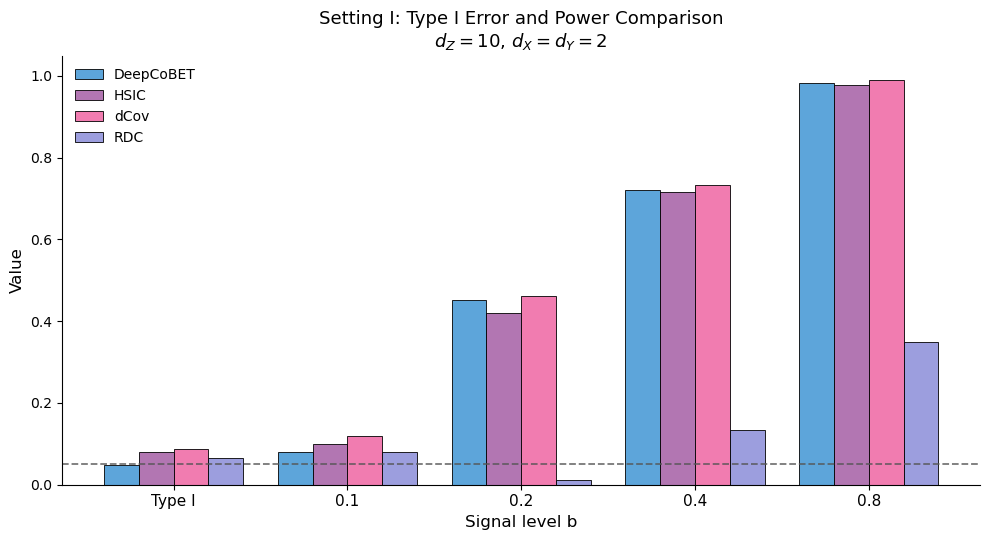
\includegraphics[
            width=\linewidth,
            alt={Empirical size and power comparison of DeepCoBET, HSIC,
            distance covariance, and RDC under simulation Setting 1
            with dimension 2.}
        ]{plots/CI_setting1_dim2.png}
        \caption{$\dim(X)=\dim(Y)=2$}
    \end{subfigure}
    \hfill
    \begin{subfigure}[t]{0.48\textwidth}
        \centering
        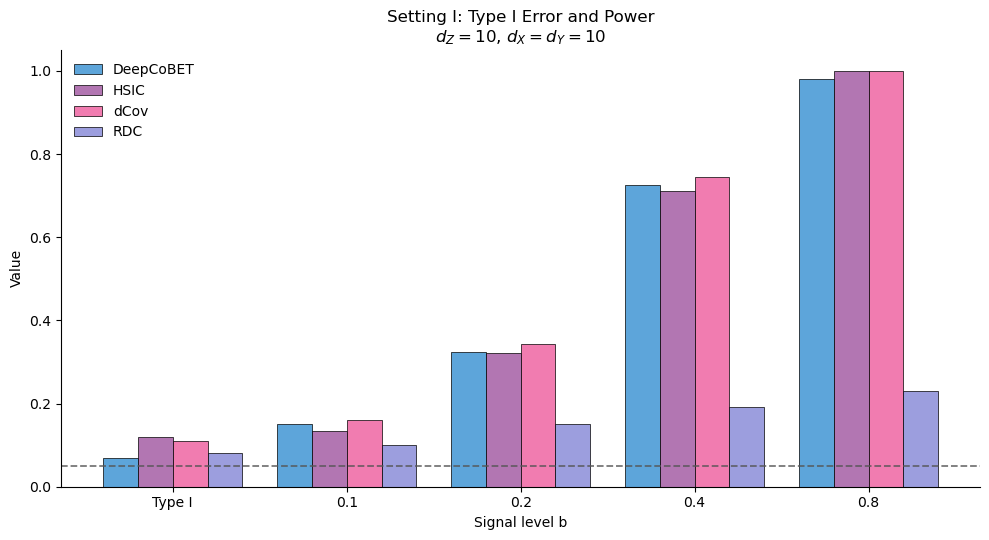
\includegraphics[width=\linewidth, alt={Empirical size and power comparison of DeepCoBET, HSIC, distance covariance, and RDC under simulation Setting 1 with dimension 10.}]{plots/CI_setting1_dim10.png}
        \caption{$\dim(X)=\dim(Y)=10$}
    \end{subfigure}

    \caption{Empirical size and power comparison of DeepCoBET, HSIC, dCov, and RDC
    under Setting I for two dimensional configurations.}
    \label{fig:setting1-combined}
\end{figure}

\begin{figure}[htbp]
    \centering

    \begin{subfigure}[t]{0.48\textwidth}
        \centering
        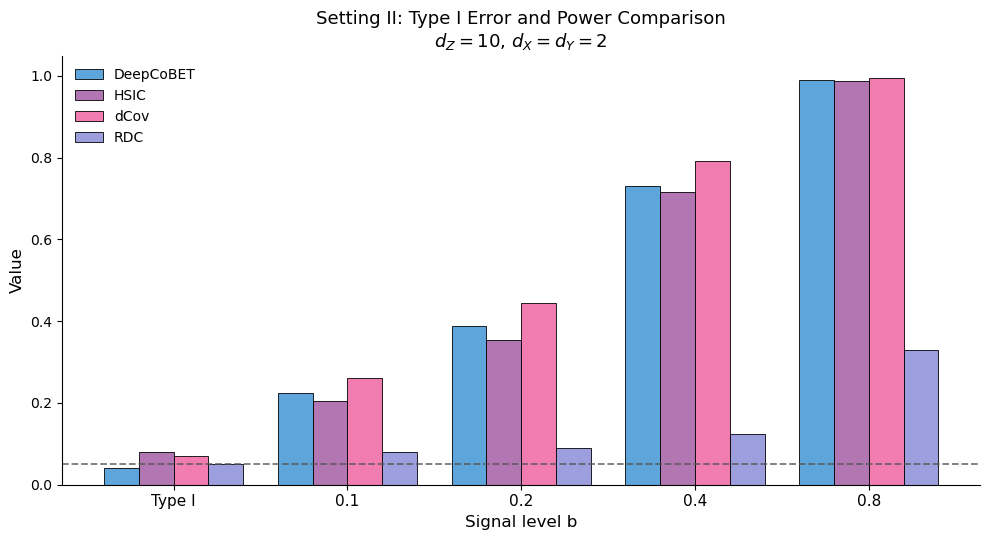
\includegraphics[width=\linewidth, alt={Empirical size and power comparison of DeepCoBET, HSIC,
            distance covariance, and RDC under simulation Setting 2
            with dimension 2.}]{plots/CI_setting2_dim2.png}
        \caption{$\dim(X)=\dim(Y)=2$}
    \end{subfigure}
    \hfill
    \begin{subfigure}[t]{0.48\textwidth}
        \centering
        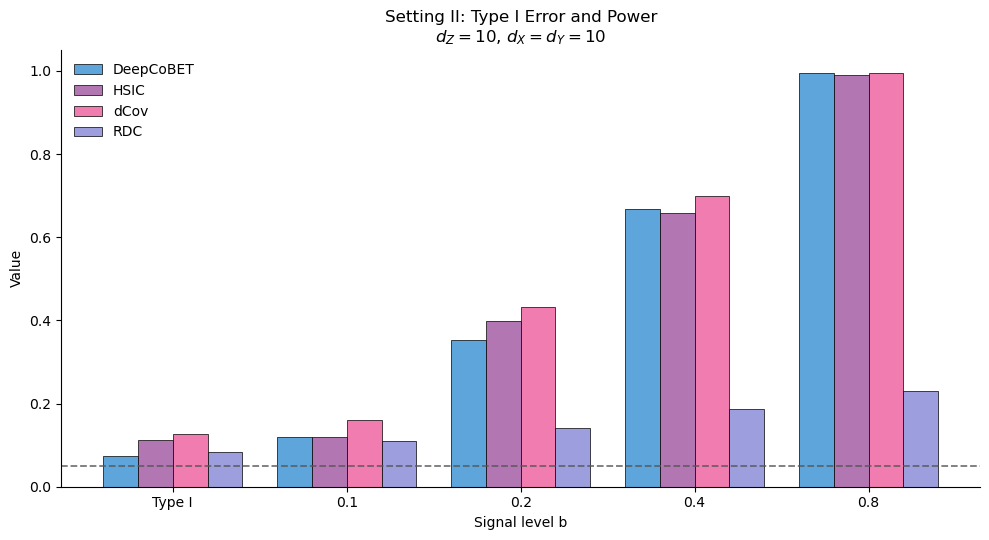
\includegraphics[width=\linewidth, alt={Empirical size and power comparison of DeepCoBET, HSIC,
            distance covariance, and RDC under simulation Setting 2
            with dimension 10.}]{plots/CI_setting2_dim10.png}
        \caption{$\dim(X)=\dim(Y)=10$}
    \end{subfigure}

    \caption{Empirical size and power comparison of DeepCoBET, HSIC, dCov, and RDC
    under Setting II for two dimensional configurations.}
    \label{fig:setting2-combined}
\end{figure}

\begin{figure}[htbp]
    \centering

    \begin{subfigure}[t]{0.48\textwidth}
        \centering
        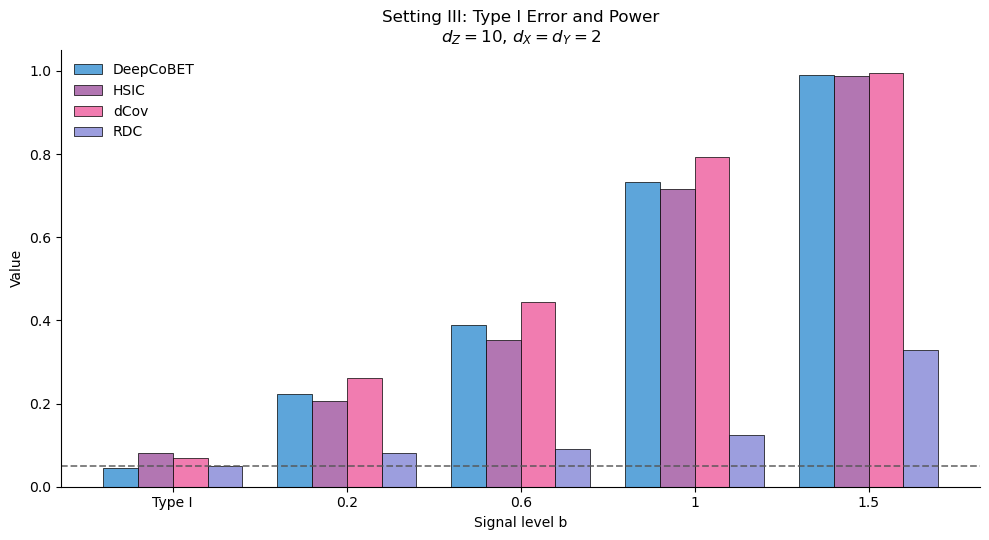
\includegraphics[width=\linewidth, alt={Empirical size and power comparison of DeepCoBET, HSIC,
            distance covariance, and RDC under simulation Setting 3
            with dimension 2.}]{plots/CI_setting3_dim2.png}
        \caption{$\dim(X)=\dim(Y)=2$}
    \end{subfigure}
    \hfill
    \begin{subfigure}[t]{0.48\textwidth}
        \centering
        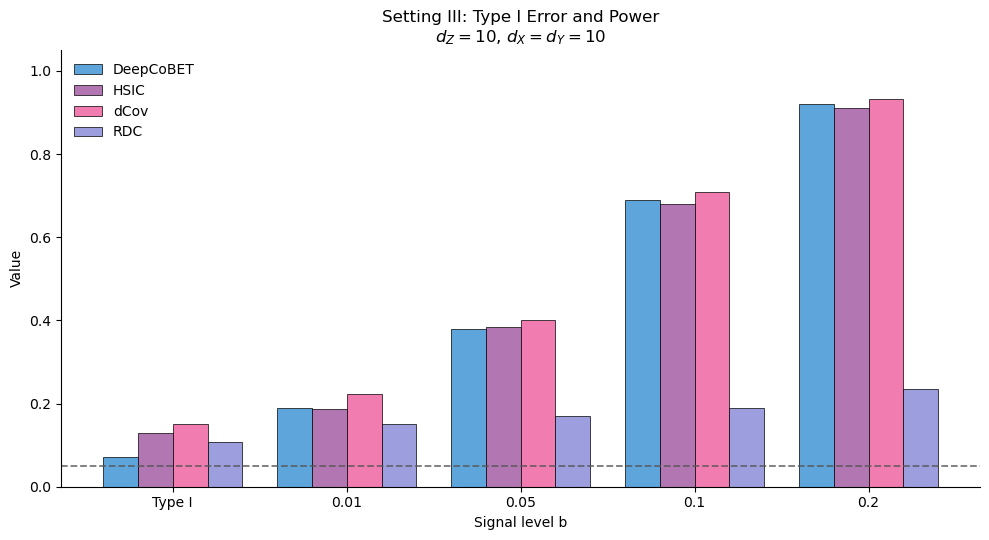
\includegraphics[width=\linewidth, alt={Empirical size and power comparison of DeepCoBET, HSIC,
            distance covariance, and RDC under simulation Setting 3
            with dimension 10.}]{plots/CI_setting3_dim10.png}
        \caption{$\dim(X)=\dim(Y)=10$}
    \end{subfigure}

    \caption{Empirical size and power comparison of DeepCoBET, HSIC, dCov, and RDC
    under Setting III for two dimensional configurations.}
    \label{fig:setting3-combined}
\end{figure}

\section{Real World Application}
\label{sec:realdata_eye_conditional}

\subsection{Conditional dependence analysis via DeepCoBET}
\label{sec:realdata_eye_conditional}

We further analyze the corneal epithelial thickness data using DeepCoBET to investigate conditional dependence patterns. The dataset arises from a dry eye disease study and contains measurements across 25 predefined corneal regions for both eyes (OD and OS) from 189 subjects, obtained via anterior segment optical coherence tomography. Each observation is represented as a spatial thickness map, where regions correspond to angular sectors and concentric rings (see Figure~\ref{fig:realdata_application}).

\begin{figure}[!t]
    \centering
    \begin{subfigure}[b]{0.47\columnwidth}
        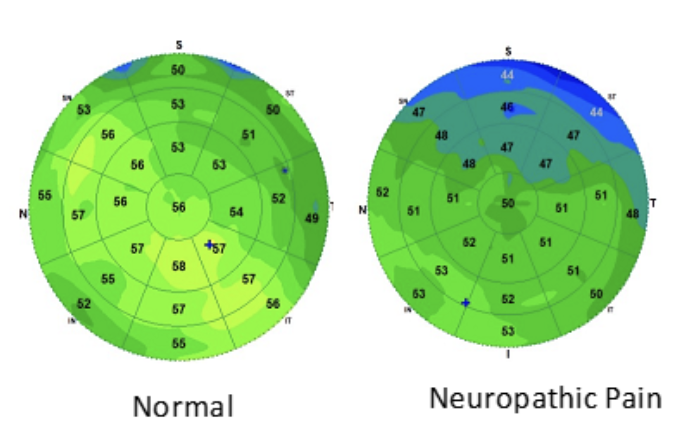
\includegraphics[
            width=\textwidth,
            height=0.22\textheight,
            keepaspectratio, alt={Representative corneal epithelial thickness map showing
the spatial arrangement of the central, inner, middle, and
outer corneal regions analyzed in the study.}
        ]{plots/DED_1.png}
    \end{subfigure}
    \hspace{-0.1em}
    \begin{subfigure}[b]{0.47\columnwidth}
        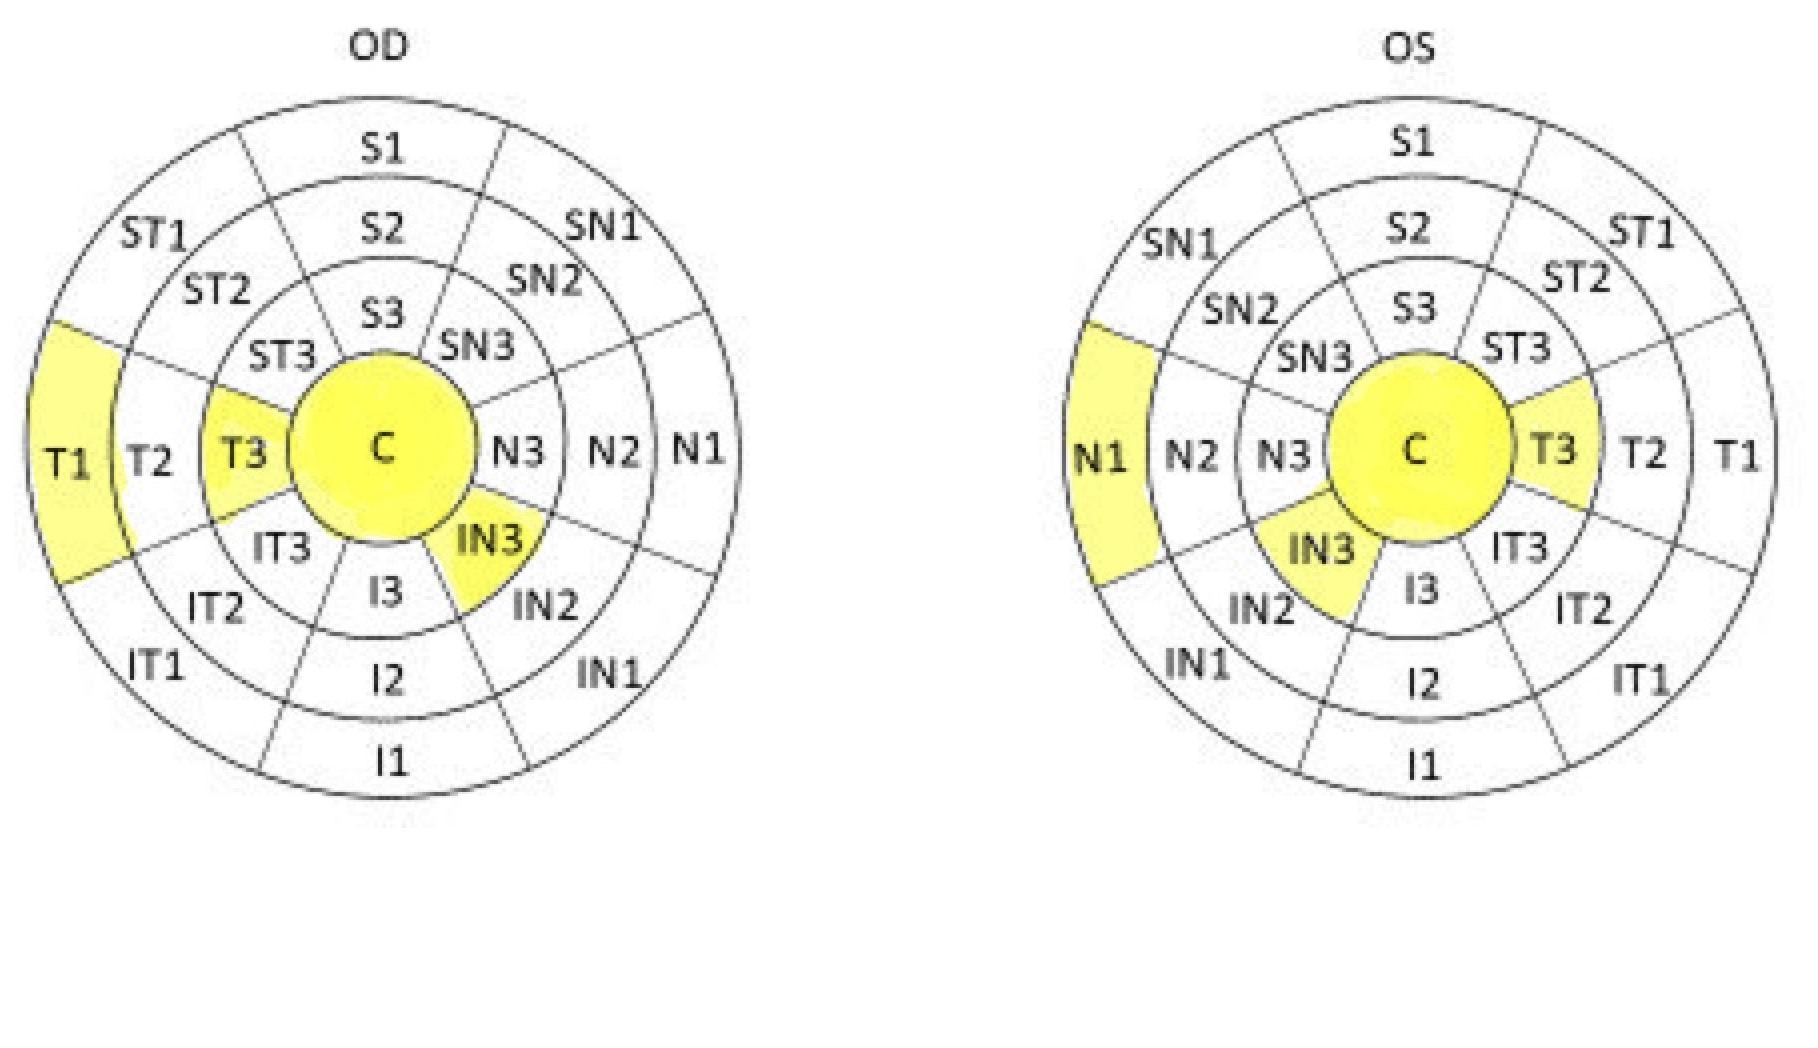
\includegraphics[
            width=\textwidth,
            height=0.22\textheight,
            keepaspectratio, alt={Corneal regional map from the DeepCoBET analysis with
highlighted regions indicating statistically significant
conditional dependence between the left and right eyes.}
        ]{plots/DeepCoBET_real_example.png}
    \end{subfigure}
    \caption{\scriptsize
    \textbf{Left:} Representative corneal epithelial thickness maps, where darker regions indicate thinner epithelium.
    \textbf{Right:} Regional partition used for dependence analysis, with highlighted regions indicating statistically significant dependence between the left and right eyes.
    }
    \label{fig:realdata_application}
    \vspace{-0.8em}
\end{figure}

In contrast to the marginal analysis in Section~\ref{sec:realdata_eye}, where strong and widespread dependence was observed across nearly all regions, we now examine whether these relationships persist after adjusting for shared structural and clinical factors.

We consider several clinically relevant variables as part of the conditioning set, including the Schirmer test (tear production), \emph{HOA - total} (total higher-order aberrations, reflecting corneal optical irregularities), and \emph{logMAR} (a standard measure of visual acuity). These variables capture important physiological characteristics that may induce apparent dependence between the two eyes.

The conditioning set $Z$ is constructed in a \emph{region-specific} manner. For each concentric section, $Z$ includes all corneal regions outside the section of interest, together with the clinical variables. Specifically:
(i) for the central region plus inner ring, $Z$ consists of the middle and outer ring measurements along with Schirmer, HOA, and logMAR;
(ii) for the middle ring, $Z$ consists of the inner and outer ring measurements along with the clinical covariates;
(iii) for the outer ring, $Z$ consists of the inner and middle ring measurements along with the clinical covariates.
This design removes global structural effects and allows us to isolate residual dependence specific to each region.

Following the DeepCoBET framework, we estimate conditional expectations of each regional measurement given $Z$ using cross-fitted neural networks, and compute residuals for both OD and OS. The CoBET statistic is then applied to these residuals to test for conditional dependence.

Figure~\ref{fig:eye_heatmaps_conditional} presents the resulting dependence heatmaps. Compared to the unconditional results, where nearly all region pairs exhibited significant dependence, the conditional analysis reveals a substantial reduction in significant signals. This indicates that much of the apparent bilateral dependence can be explained by shared anatomical structure and common clinical factors.

In the central region plus inner ring ($p=q=10$), only a small number of region pairs remain significant, including the central region (C), the variability measure (EStd Dev), and specific cross-regional interactions such as C with T3. These residual signals suggest that localized dependence in the central cornea cannot be fully explained by global structure or observed covariates, and may reflect intrinsic bilateral coordination near the visual axis.

In contrast, the middle ring ($p=q=8$) exhibits no statistically significant dependence after conditioning. This implies that the dependence observed in the marginal analysis is largely driven by surrounding regions and shared physiological factors, rather than direct coupling between corresponding regions.

For the outer ring ($p=q=8$), only a single significant interaction is detected, corresponding to T1 versus N1. This isolated signal indicates that peripheral dependence is weak and highly localized, potentially reflecting subtle asymmetries in environmental exposure or increased measurement variability at the corneal boundary.

Overall, the conditional analysis reveals a markedly sparser and more localized dependence structure compared to the marginal case. While the unconditional analysis suggests strong bilateral symmetry across all regions, the DeepCoBET results demonstrate that this symmetry is largely attributable to shared structural and clinical influences. After adjustment, the remaining dependence is concentrated in a few specific regions, highlighting the importance of conditional testing in uncovering interpretable and biologically meaningful relationships.
\begin{figure}[!t]
    \centering

    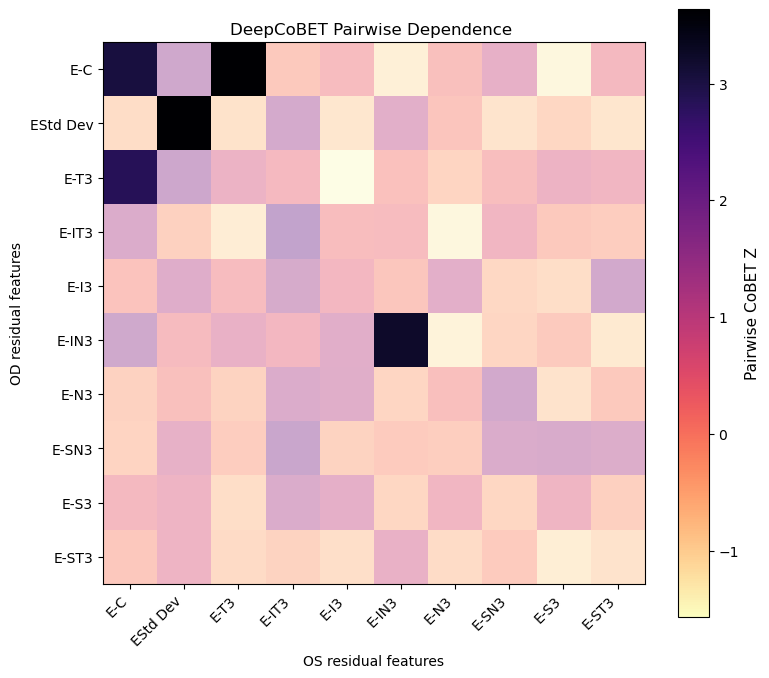
\includegraphics[
      trim=14pt 12pt 14pt 12pt,clip,
      width=0.34\columnwidth,height=0.2\textheight,keepaspectratio, alt={Conditional dependence heatmap for the central and inner
corneal regions, showing a small number of significant
region pairs after adjustment for clinical covariates.}
    ]{plots/DeepCoBET_inner.png}\hspace{-0.6em}%
    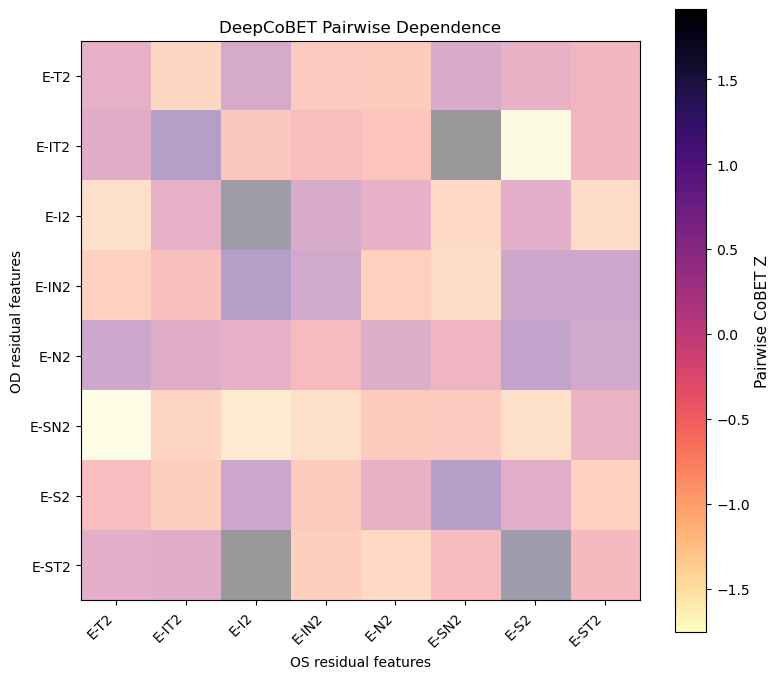
\includegraphics[
      trim=14pt 12pt 14pt 12pt,clip,
      width=0.34\columnwidth,height=0.2\textheight,keepaspectratio, alt={Conditional dependence heatmap for the middle corneal ring,
showing no significant region pairs after adjustment for
clinical covariates.}
    ]{plots/DeepCoBET_middle.png}\hspace{-0.6em}%
    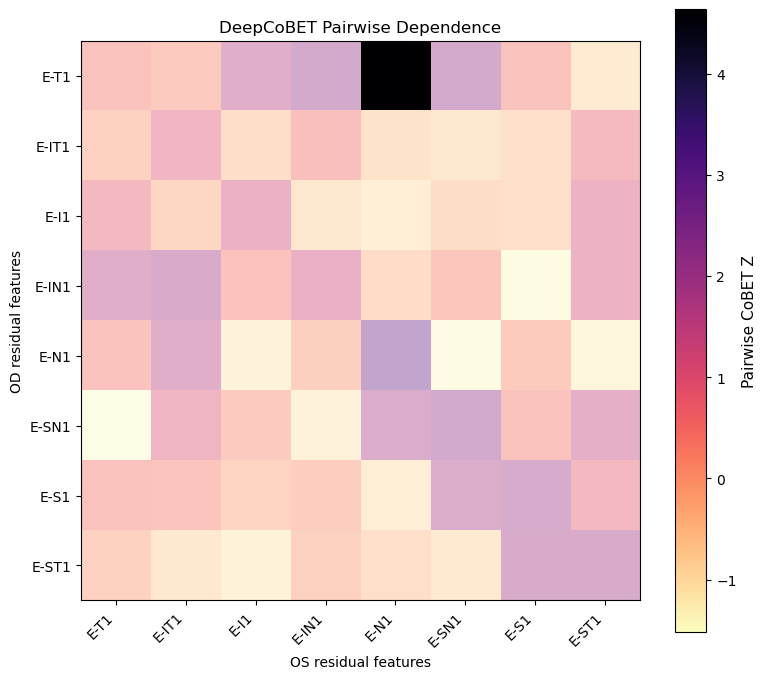
\includegraphics[
      trim=14pt 12pt 14pt 12pt,clip,
      width=0.34\columnwidth,height=0.2\textheight,keepaspectratio, alt={Conditional dependence heatmap for the outer corneal ring,
showing one localized significant interaction after adjustment
for clinical covariates.}
    ]{plots/DeepCoBET_outer.png}

    \caption{\scriptsize
    DeepCoBET conditional dependence heatmaps for corneal epithelial thickness regions, X-axis is the OD regions and Y-axis is the OS regions:
    left: Section~1 ($p=q=10$; central + inner ring); middle: Section~2 ($p=q=8$; middle ring);
    right: Section~3 ($p=q=8$; outer ring).
    After adjusting for tear production (Schirmer test), higher-order aberrations (HOA), and visual acuity (logMAR), the dependence structure becomes substantially sparser. Only a few localized signals remain in the central region, no significant dependence is observed in the middle ring, and a single peripheral interaction is detected in the outer ring.
    }
    \label{fig:eye_heatmaps_conditional}
    \vspace{-0.6em}
\end{figure}

\section{Conclusion}

In this chapter, we developed a unified framework for multivariate conditional
independence testing based on deep residualization and binary expansion
representations. The proposed DeepCoBET procedure combines the flexibility of
neural network-based conditional modeling with the interpretability and
multiscale structure of the CoBET framework, providing a powerful and
computationally efficient approach for detecting nonlinear and high-dimensional
dependencies.

The simulation studies demonstrate that DeepCoBET achieves reliable Type~I
error control and strong power across a wide range of data-generating
mechanisms, including linear and highly nonlinear settings. The method remains
robust as the dimensionality of $X$ and $Y$ increases, consistently exhibiting
performance comparable to or better than state-of-the-art methods such as HSIC
and distance covariance, while substantially outperforming RDC. These results
highlight the ability of DeepCoBET to effectively capture complex dependence
structures without sacrificing statistical validity.

The real-data application further illustrates the practical value of the
proposed framework. By applying DeepCoBET to corneal epithelial thickness data,
we showed that conditional analysis can substantially refine the understanding
of dependence structures. While marginal analysis suggests widespread bilateral
symmetry, the conditional results reveal that most of this dependence can be
explained by shared anatomical and clinical factors. After adjustment, only a
small number of localized interactions remain significant, particularly in the
central corneal region. This demonstrates that DeepCoBET is not only effective
for hypothesis testing, but also provides interpretable insights into the
underlying structure of complex biomedical data.

Overall, the proposed DeepCoBET framework offers a flexible and scalable
solution to multivariate conditional independence testing. By integrating
modern machine learning techniques with a principled statistical testing
framework, it addresses key challenges in high-dimensional settings and enables
more accurate and interpretable inference in practical applications.
\chapter{Conclusion and Future Work}

\section{Conclusion}

Testing statistical independence is a fundamental problem in statistics and machine learning, with wide applications in causal inference, graphical models, and high-dimensional data analysis. This dissertation develops a unified framework for testing both marginal independence and conditional independence for multivariate variables, with particular emphasis on high-dimensional settings and complex nonlinear relationships. The proposed methods combine ideas from binary expansion representations, U-statistic theory, and modern deep learning techniques, resulting in flexible and computationally efficient procedures with strong theoretical guarantees.

The first part of this dissertation introduces a new class of nonparametric tests for multivariate independence, including the Covariance Binary Expansion Test (CoBET), its distance-based extension dCoBET, and an adaptive aggregation method wa-dCoBET. The key idea is to represent dependence structures through binary expansion interaction coefficients, transforming the independence testing problem into testing cross-covariances among these coefficients. Although the number of possible interactions grows exponentially with dimension, we show that the resulting statistics can be expressed as U-statistics with explicit kernel representations, enabling efficient computation and theoretical analysis.

The proposed tests are distribution-free and automatically adapt to unknown dependence structures through multiscale truncation of higher-order interactions. In addition, the binary expansion framework provides interpretability by identifying the interaction components responsible for detected dependence. To further enhance statistical power and computational efficiency, we develop an adaptive weighted aggregation procedure, wa-dCoBET, which combines complementary test statistics derived from covariance-based and distance-based binary expansion representations. Extensive simulation studies and real-data applications demonstrate that the proposed methods consistently achieve competitive or superior performance compared with existing approaches such as HSIC and distance covariance, particularly in higher-dimensional and non-monotone dependence settings while maintaining accurate type I error control.

The second part of this dissertation addresses the problem of conditional independence testing. In many modern applications, the confounding variable $Z$ may be high-dimensional, which poses significant challenges for traditional nonparametric methods due to the curse of dimensionality. To address this issue, we propose a hybrid framework, DeepBET, which integrates deep neural networks (DNNs) with binary expansion testing (BET). In this approach, DNN models are used to estimate the conditional mean functions of $X$ given $Z$ and $Y$ given $Z$, effectively removing the influence of high-dimensional confounding variables.

After estimating these conditional expectations, BET statistics are applied to the residuals to test for remaining dependence. To improve stability and statistical power, we incorporate a multi-split procedure that repeatedly partitions the data and aggregates the resulting test statistics. The DeepBET procedure effectively controls the type I error and demonstrates strong power under complex nonlinear alternatives. Moreover, the binary expansion representation provides interpretable insights into the form of the detected conditional dependence, which can be useful for subsequent modeling and scientific interpretation.

Building on these developments, the final part of this dissertation studies the more general problem of multivariate conditional independence testing, where both $X$ and $Y$ are multivariate random vectors and the conditioning variable $Z$ may be high-dimensional. In this setting, deep neural networks are first used to estimate the conditional expectations of $X$ and $Y$ given $Z$. The resulting residual vectors are then analyzed using the multivariate independence testing framework developed earlier in this dissertation CoBET. This strategy combines the flexibility of deep learning for modeling complex conditional relationships with the interpretability and statistical power of binary expansion–based independence tests.

Overall, this dissertation contributes a comprehensive methodology for independence and conditional independence testing that addresses several important challenges in modern data analysis, including high dimensionality, nonlinear dependence structures, and multivariate interactions. The proposed framework bridges classical statistical theory with modern machine learning techniques, providing both theoretical insight and practical tools for dependence analysis in complex data environments.

\section{Future Work}

While the methods developed in this dissertation provide effective solutions for a variety of independence testing problems, several promising research directions remain for future investigation.%\footnote{may be you can add a future work for conditional independent test using the idea of Binary Expansion Group Interaction Network. \url{https://arxiv.org/abs/2603.24763}}

\subsection{Direct Conditional Independence Testing via Binary Expansion Group Intersection Networks}

The conditional independence procedures developed in this dissertation are
based on a residualization strategy. Specifically, conditional independence is
reduced to an unconditional independence problem by first estimating the
conditional mean functions using deep neural networks and subsequently applying
binary expansion-based independence tests to the estimated residuals. While
this approach performs well in high-dimensional settings, its theoretical and
empirical performance depends on the quality of the regression estimators.

A promising direction for future research is to develop conditional
independence tests that operate directly on binary expansion representations
without an explicit residualization step. Recent work by
\citet{zhou2026binaryexpansiongroupintersection} introduced the Binary Expansion Group Intersection
Network (BEGIN), a distribution-free graphical representation of conditional
independence based on binary interaction features. The central result of BEGIN
establishes that, for multivariate binary variables and bit-encoded
multinomial variables, conditional independence can be characterized exactly
through the covariance structure of binary interaction terms. Moreover, the
authors show that dyadic binary representations provide increasingly accurate
approximations for general continuous random vectors under mild regularity
conditions. \citep{zhou2026binaryexpansiongroupintersection}

These results suggest a new avenue for extending the binary expansion
framework developed in this dissertation. Rather than estimating residuals and
testing their independence, one could directly construct test statistics from
the covariance structure associated with BEGIN. Such procedures may provide a
fully nonparametric and distribution-free approach to conditional independence
testing that avoids the challenges of estimating high-dimensional regression
functions. In addition, the graphical representation induced by BEGIN offers
the possibility of identifying which binary interaction components are
responsible for conditional dependence, thereby providing substantially greater
interpretability than existing black-box methods.

More broadly, the combination of BEGIN and the binary expansion methodology
developed in this dissertation may lead to a unified framework for
independence testing, conditional independence testing, graphical model
estimation, and causal structure learning. Investigating the statistical
properties, computational scalability, and high-dimensional behavior of such
procedures represents an important direction for future research.


\subsection{Independence Testing for Modern Machine Learning Models} Recent developments in large-scale machine learning models raise new questions about independence testing in the context of model parameters and learned representations. In particular, recent work by \citet{zhu2025independence} studies the problem of determining whether two neural network models were trained independently by analyzing their learned weights. The authors formulate a hypothesis testing problem in which the null hypothesis states that the parameters of two models are independent, corresponding to the case where the models were trained from independent random initializations. Under this framework, dependence may arise when one model is derived from another through procedures such as fine-tuning, pruning, or distillation. In the constrained setting considered in \citet{zhu2025independence}, assumptions are made about the training procedure and model architecture that allow the construction of exact $p$-values. In particular, if the training algorithm is equivariant to permutations of hidden units at initialization, then exchangeable copies of model weights can be simulated and used to construct permutation-based independence tests. These tests compare similarity measures between the original pair of models with those obtained from the simulated copies, allowing reliable detection of dependence between models. The authors also consider an unconstrained setting in which the training assumptions may not hold, such as when adversarial modifications or architectural changes are introduced. In this case, hidden representations between models are first aligned before computing similarity measures between the aligned components to detect dependence. This approach can even localize which parts of a model are derived from another, providing insight into relationships between large language models. These recent developments highlight a new application domain for independence testing beyond traditional statistical data analysis. In future work, it would be interesting to explore whether the binary expansion framework developed in this dissertation can be extended to analyze dependence between neural network parameters or internal representations. In particular, the multiscale interaction structure underlying CoBET and its extensions may provide new ways to detect subtle dependencies among high-dimensional model weights or learned feature representations. Such tools could contribute to emerging areas such as model provenance analysis, intellectual property protection for machine learning models, and auditing of large-scale AI systems.

\subsection{Conditional Independence Testing for Sequential Data}

Many real-world datasets involve sequential or time-dependent observations, such as financial time series, climate systems, biological signals, and language data. In such settings, dependence structures evolve over time and the classical assumption of independent and identically distributed observations may no longer hold. As a result, extending conditional independence testing methods to sequential data represents an important direction for future research.

Recent work in causal discovery for time series has emphasized the role of conditional independence tests in identifying causal relationships among temporally ordered variables. For example, the PCMCI framework proposed by \citet{runge2019detecting} combines conditional independence tests with a constraint-based causal discovery algorithm to estimate causal networks from large-scale time series data. The method addresses challenges such as strong autocorrelation and high dimensionality by carefully selecting conditioning sets and exploiting temporal ordering.

Subsequent developments such as PCMCI$^{+}$ further extend this framework to detect both lagged and contemporaneous causal relations in nonlinear and autocorrelated time series datasets \citep{runge2020discovering}. These approaches demonstrate that conditional independence testing can play a central role in learning causal structures from sequential data.

Extending the methods developed in this dissertation to sequential settings would therefore be a promising research direction. One potential approach is to integrate the proposed binary expansion–based testing framework with models designed for sequential data, such as recurrent neural networks, temporal convolutional networks, or transformer architectures. These models could first estimate conditional relationships across time, after which independence testing procedures such as CoBET and its extensions could be applied to the resulting residual processes.

Developing such methods could broaden the applicability of binary expansion testing to important domains including time-series causal discovery, reinforcement learning, and dynamic graphical models.


\subsection{Extensions to Structured and Multi-Modal Data}

Another promising direction is to extend the proposed testing framework to more complex data types, including structured data, graph data, image data, and multi-modal datasets. In many modern applications, variables may represent complex objects rather than simple vectors. Developing binary expansion representations and independence tests tailored to these data structures could significantly broaden the applicability of the proposed methodology.

\subsection{Applications to Causal Discovery}

Independence and conditional independence tests are essential components of many causal discovery algorithms. The proposed testing framework could therefore be incorporated into constraint-based causal discovery methods to improve their performance in high-dimensional and nonlinear settings. Potential application areas include genomics, biomedical research, economics, and other scientific fields where complex dependence structures commonly arise.

\section{Final Remarks}

This dissertation develops a unified framework for independence and conditional independence testing by combining multiscale statistical representations with modern machine learning techniques. The proposed methods demonstrate that binary expansion–based testing can be effectively integrated with deep neural network models to address challenging high-dimensional problems. These approaches provide flexible, interpretable, and computationally efficient tools for detecting complex dependence structures in modern datasets.

The future research directions outlined above highlight many opportunities for extending this framework and further advancing the theory and applications of independence testing in statistics and machine learning.
\backmatter
\singlespacing

\bibliographystyle{plainnat}
\bibliography{references}

% Publication agreements
% =================================================
% APPENDIX: PUBLICATION AGREEMENTS
% =================================================

\chapter*{Appendix}
\addcontentsline{toc}{chapter}{Appendix}

\begin{center}
\textbf{Publication Agreements}
\end{center}

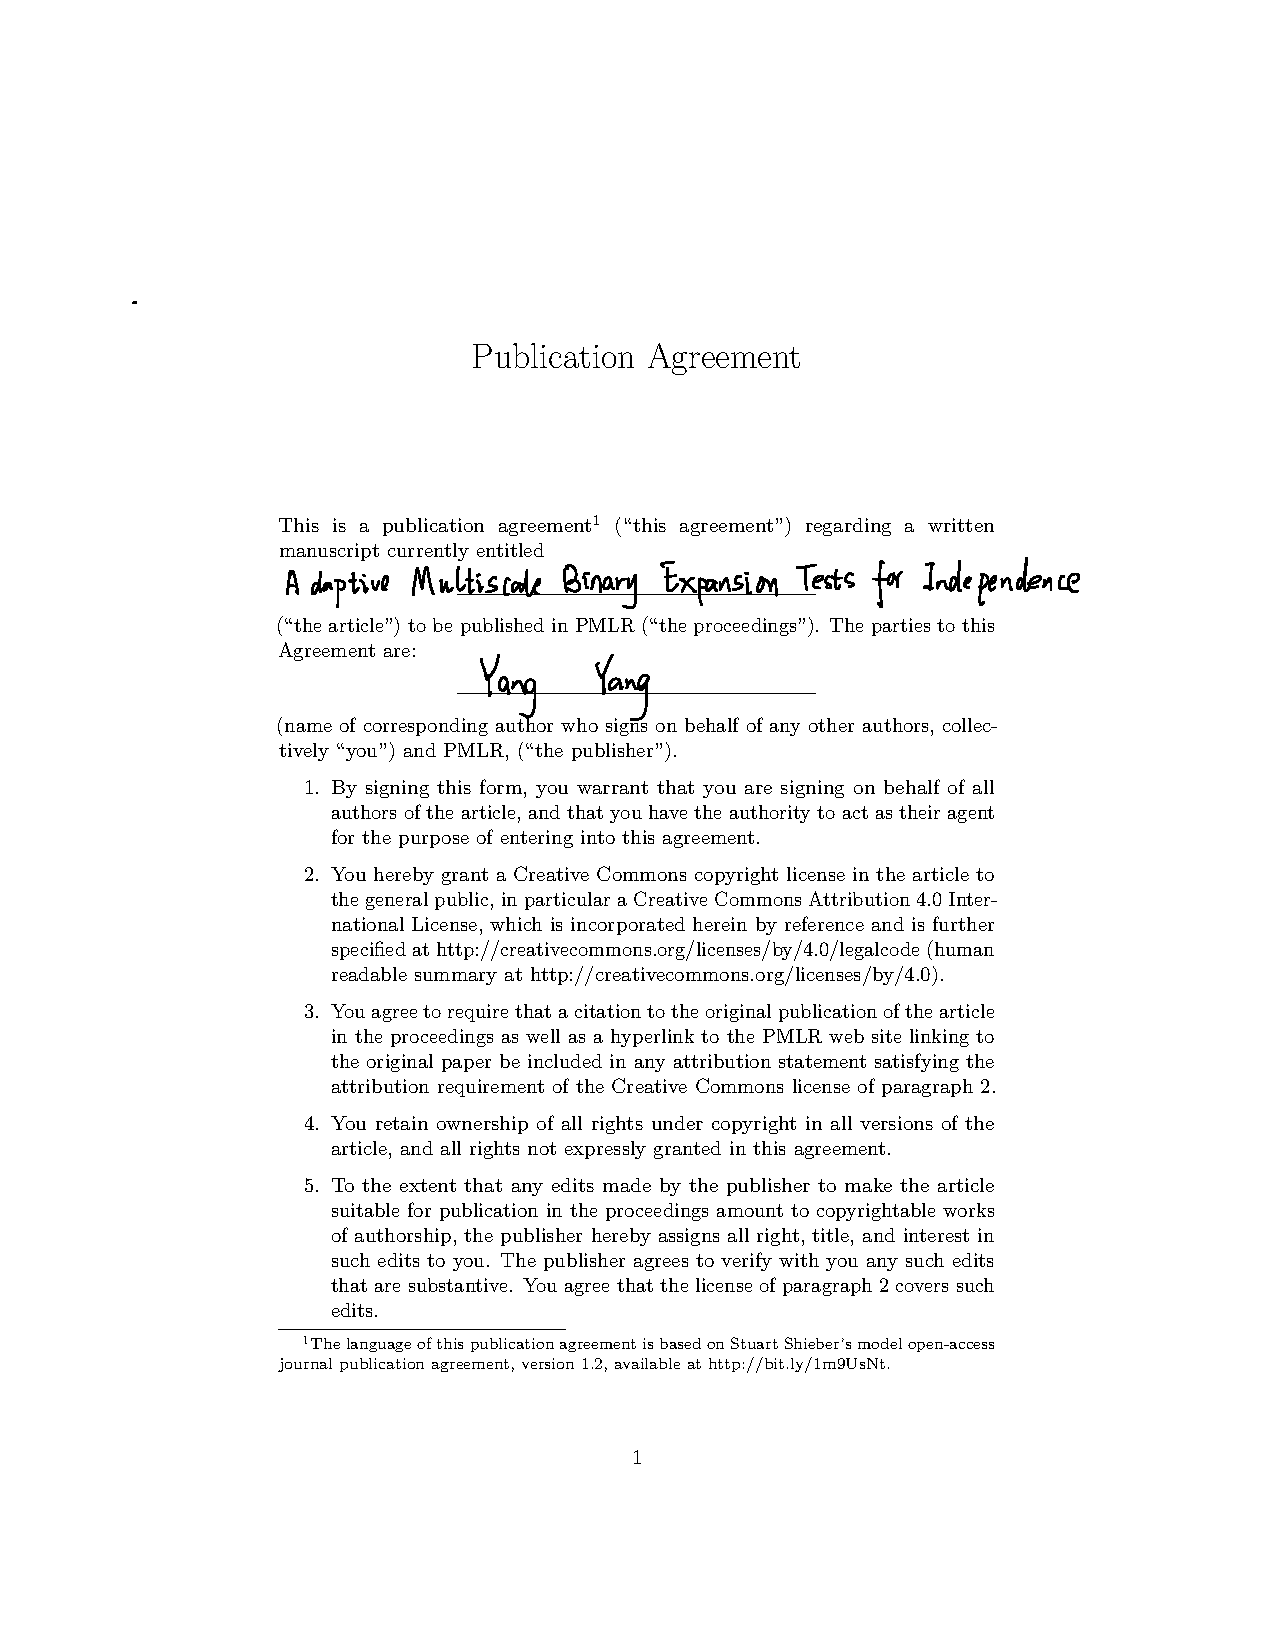
\includepdf[
    pages=-,
    pagecommand={\thispagestyle{plain}}
]{ICML_Copyright.pdf}

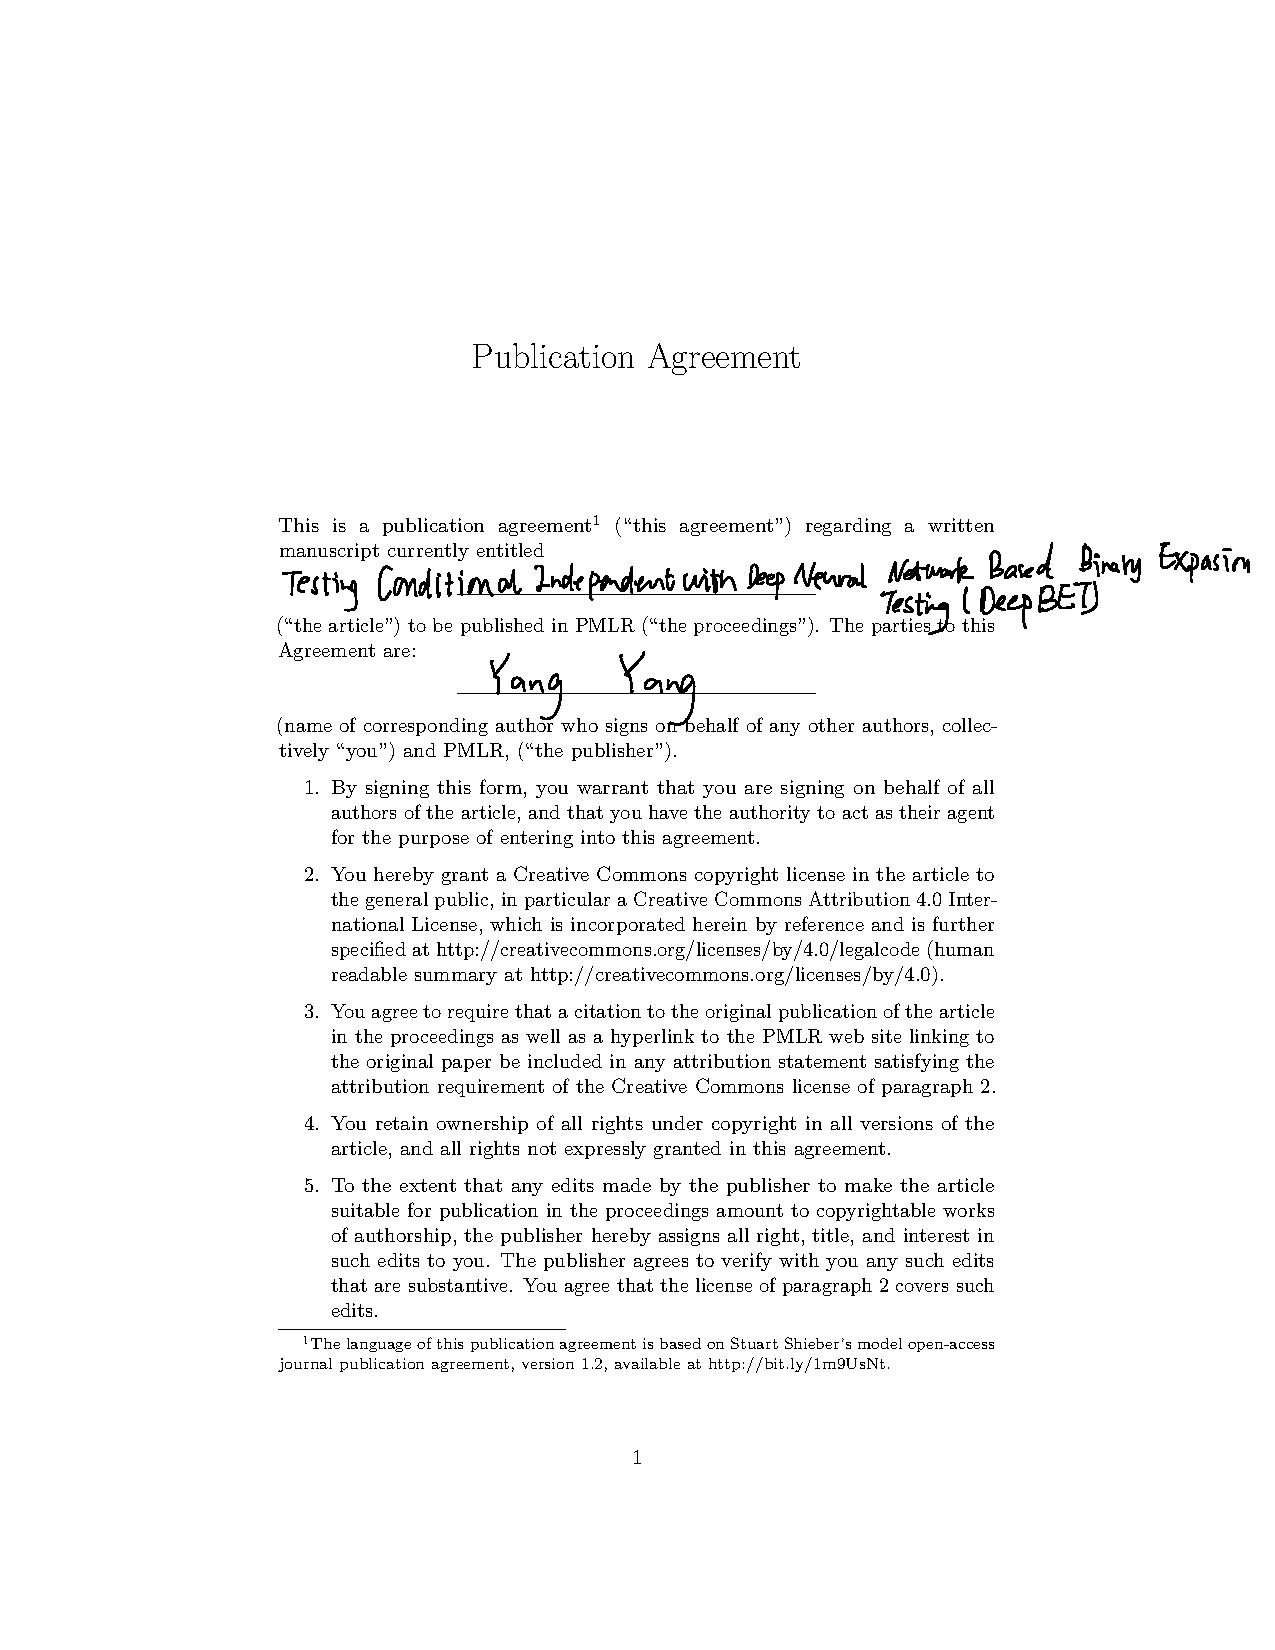
\includepdf[
    pages=-,
    pagecommand={\thispagestyle{plain}}
]{DeepBET_Copyright.pdf}
% publication agreements go here

% =================================================
% VITA
% =================================================

\cleardoublepage
\chapter*{VITA}
\addcontentsline{toc}{chapter}{VITA}

\noindent
\textbf{Yang Yang}

\vspace{0.5cm}

\noindent
\textbf{EDUCATION}

\begin{itemize}
    \item Ph.D. in Mathematics, University of Illinois Chicago, 2026.
    \item M.S. in Marketing Analytics and Communication, Illinois Institute of Technology, 2014.
    \item B.Eng. in Inorganic Nonmetallic Materials Engineering, University of Science and Technology Beijing, 2012.
\end{itemize}

\vspace{0.3cm}
\noindent
\textbf{PUBLICATIONS}

\begin{itemize}

    \item Yang, Y., Zhang, K., and Zhong, P.-S.
    ``Testing Conditional Independence with Deep Neural Network Based
    Binary Expansion Testing (DeepBET).''
    \textit{Proceedings of the 28th International Conference on
    Artificial Intelligence and Statistics (AISTATS)}, 2025.

    \item Yang, Y., Zhong, P.-S., and Zhang, K.
    ``Adaptive Multiscale Binary Expansion Tests for Independence.''
    \textit{International Conference on Machine Learning (ICML)}, 2026.

    \item Katz, E. A., Yang, Y., Surenkhuu, B., Dabre, Z., Dammak, A.,
    Rao, V. R., Mun, C., Pradeep, A., Kim, C., Aref, A. A., Bhat, P.,
    de la Cruz, J., Kaja, S., and Jain, S.
    ``Neutrophil Extracellular Trap Components Are Present in the
    Aqueous Humor of Glaucoma Patients.''
    \textit{Translational Vision Science \& Technology}.

    \item Dabre, Z. G., Bernal, A., Yang, Y., Surenkhuu, B., Mun, J.,
    Hernandez, D., Pradeep, A., Sheth, T., Kim, C., Zhong, P.-S.,
    Byrne, K., Mun, C., and Jain, S.
    ``Corneal Epithelial Thickness: A Marker for Auto-immune Dry Eye Disease.''
    \textit{The Ocular Surface}, under review.

\end{itemize}



\vspace{0.3cm}

\noindent
\textbf{SELECTED CONFERENCE PRESENTATIONS}

\begin{itemize}

    \item Poster, ``Adaptive Multiscale Binary Expansion Tests for
    Independence,'' International Conference on Machine Learning
    (ICML), 2026.

    \item Poster, ``Testing Conditional Independence with Deep Neural
    Network Based Binary Expansion Testing (DeepBET),''
    International Conference on Artificial Intelligence and Statistics
    (AISTATS), 2025.

    \item Talk, ``Conditional Independence with Deep Neural Network
    Based Binary Expansion Test (DeepBET),''
    Joint Statistical Meetings (JSM), Portland, Oregon, 2024.

    \item Talk, ``Conditional Independence with Deep Neural Network
    Based Binary Expansion Test (DeepBET),''
    WNAR/IMS/Graybill Annual Meeting, Colorado, 2024.

    \item Session Chair, ``Recent Advances in Statistical Inference
    and Their Applications,'' WNAR/IMS/Graybill Annual Meeting,
    Colorado, 2024.

\end{itemize}

\vspace{0.3cm}

\noindent
\textbf{PROFESSIONAL AND ACADEMIC EXPERIENCE}

\begin{itemize}
    \item Research Assistant, University of Illinois Chicago, Department of Mathematics, Statistics, and Computer Science,
    2023--2026.
    \item Teaching Assistant, University of Illinois Chicago,
    Department of Mathematics, Statistics, and Computer Science,
    2020--2023.
    \item Biostatistician Intern, Edwards Lifesciences, 2024.

    \item Data Scientist Intern, Schnucks, 2023.

\end{itemize}



\end{document}
